%% USPSC-modelo-EESC.tex
% ---------------------------------------------------------------
% USPSC: Modelo de Trabalho Academico (tese de doutorado, dissertacao de
% mestrado e trabalhos monograficos em geral) em conformidade com 
% ABNT NBR 14724:2011: Informacao e documentacao - Trabalhos academicos -
% Apresentacao
%----------------------------------------------------------------
%% Esta é uma customização do abntex2-modelo-trabalho-academico.tex de v-1.9.5 laurocesar 
%% para as Unidades do Campus USP de São Carlos:
%% EESC - Escola de Engenharia de São Carlos
%% IAU - Instituto de Arquitetura e Urbanismo
%% ICMC - Instituto de Ciências Matemáticas e de Computação
%% IFSC - Instituto de Física de São Carlos
%% IQSC - Instituto de Química de São Carlos
%%
%% Este trabalho utiliza a classe USPSC.cls que é mantida pela seguinte equipe:
%% 
%% Coordenação e Programação:
%%   - Marilza Aparecida Rodrigues Tognetti - marilza@sc.usp.br (PUSP-SC)
%%   - Ana Paula Aparecida Calabrez - aninha@sc.usp.br (PUSP-SC)
%% Normalização:
%%   - Brianda de Oliveira Ordonho Sigolo - brianda@usp.br (IAU)
%%   - Eduardo Graziosi Silva - edu.gs@sc.usp.br (EESC)
%%   - Eliana de Cássia Aquareli Cordeiro - eliana@iqsc.usp.br (IQSC)
%%   - Flávia Helena Cassin - cassinp@sc.usp.br (EESC)
%%   - Maria Cristina Cavarette Dziabas - mcdziaba@ifsc.usp.br (IFSC)
%%   - Regina Célia Vidal Medeiros - rcvmat@icmc.usp.br (ICMC)
%%
%% O USPSC-modelo.tex e USPSC-TCC-modelo.tex utilizam diversos arquivos relacionado em 
%% 2.1 Pacote USPSC: Classe USPSC e modelos de trabalhos acadêmicos	do Tutorial do Pascote 
%%  USPSC para modelos de trabalhos de acadêmicos em LaTeX - versão 3.1


%----------------------------------------------------------------
%% Sobre a classe abntex2.cls:
%% abntex2.cls, v-1.9.5 laurocesar
%% Copyright 2012-2015 by abnTeX2 group at https://www.abntex.net.br/ 
%%
%----------------------------------------------------------------

\documentclass[
% -- opções da classe memoir --
12pt,		% tamanho da fonte
openright,	% capítulos começam em pág ímpar (insere página vazia caso preciso)
%twoside,  % para impressão em anverso (frente) e verso. Oposto a oneside/twoside - Nota: utilizar \imprimirfolhaderosto*
oneside, % para impressão em páginas separadas (somente anverso) -  Nota: utilizar \imprimirfolhaderosto
% inclua uma % antes do comando twoside e exclua a % antes do oneside 
a4paper,			% tamanho do papel. 
% -- opções da classe abntex2 --
chapter=TITLE,		% títulos de capítulos convertidos em letras maiúsculas
% -- opções do pacote babel --
english,			% idioma adicional para hifenização
french,				% idioma adicional para hifenização
spanish,			% idioma adicional para hifenização
brazil				% o último idioma é o principal do documento
% {USPSC-classe/USPSC} configura o cabeçalho contendo apenas o número da página
]{USPSC-classe/USPSC}
%]{USPSC-classe/USPSC1}
% Inclua % antes de ]{USPSC-classe/USPSC} e retire a % antes de %]{USPSC-classe/USPSC1} para utilizar o 
% cabeçalho diferenciado para as páginas pares e ímpares:
%- páginas ímpares: com seções ou subseções e o número da página
%- páginas pares: com o número da página e o título do capítulo 
% ---
% ---
% Pacotes básicos - Fundamentais 
% ---
\usepackage[T1]{fontenc}		% Seleção de códigos de fonte.
\usepackage[utf8]{inputenc}		% Codificação do documento (conversão automática dos acentos)
\usepackage{lmodern}			% Usa a fonte Latin Modern
% Para utilizar a fonte Times New Roman, inclua uma % no início do comando acima  "\usepackage{lmodern}"
% Abaixo, tire a % antes do comando  \usepackage{times}
%\usepackage{times}		    	% Usa a fonte Times New Roman	
% Para usar a fonte , lembre-se de tirar a % do comando %\renewcommand{\ABNTEXchapterfont}{\rmfamily}, localizado mais abaixo, logo após "Outras opções para nota de rodapé no Sistema Numérico" 						
\usepackage{lastpage}			% Usado pela Ficha catalográfica
\usepackage{indentfirst}		% Indenta o primeiro parágrafo de cada seção.
\usepackage{color}				% Controle das cores
\usepackage{graphicx}			% Inclusão de gráficos
\usepackage{float} 				% Fixa tabelas e figuras no local exato
% \usepackage{chemfig,chemmacros} % Para escrever reações químicas
\usepackage{tikz}				% Para escrever reações químicas e outros

\usetikzlibrary{matrix,shapes,arrows,positioning,chains}
\usepackage{microtype} 			% para melhorias de justificação
\usepackage{pdfpages}
\usepackage{makeidx}            % para gerar índice remissivo
\usepackage{hyphenat}           % Pacote para retirar a hifenizacao do texto
\usepackage[absolute]{textpos}  % Pacote permite o posicionamento do texto
\usepackage{eso-pic}            % Pacote para incluir imagem de fundo
\usepackage{makebox}            % Pacote para criar caixa de texto
% ---

% ---
% Pacotes de citações
% Citações padrão ABNT
% ---
% Sistemas de chamada: autor-data ou numérico.
% Sistema autor-data
\usepackage[alf, abnt-emphasize=bf, abnt-thesis-year=both, abnt-repeated-author-omit=no, abnt-last-names=abnt, abnt-etal-cite=3, abnt-etal-list=3, abnt-etal-text=it, abnt-and-type=e, abnt-doi=doi, abnt-url-package=none, abnt-verbatim-entry=no]{abntex2cite}
\bibliographystyle{USPSC-classe/abntex2-alf-USPSC}
% Se o idioma for o inglês, inclua % no comando acima e exclua o % do comando abaixo
%\bibliographystyle{USPSC-classe/abntex2-alfeng-USPSC}

% Para o IQSC, que indica todos os autores nas referências, incluir % no início dos comandos acima e retirar a % dos comandos abaixo 
%\usepackage[alf, abnt-emphasize=bf, abnt-thesis-year=both, abnt-repeated-author-omit=no, abnt-last-names=abnt, abnt-etal-cite, abnt-etal-list=0, abnt-etal-text=it, abnt-and-type=e, abnt-doi=doi, abnt-url-package=none, abnt-verbatim-entry=no]{abntex2cite} 
%\bibliographystyle{USPSC-classe/abntex2-alf-USPSC}
% Se o idioma for o inglês, exclua % no comando acima ou do comando abaixo
%\bibliographystyle{USPSC-classe/abntex2-alfeng-USPSC}

% Sistema Numérico
% Para citações numéricas, sistema adotado pelo IFSC, incluir % no início dos comandos acima e retirar a % dos comandos abaixo 
%\usepackage{cite}              % agrupa citações numéricas consecutivas
%\usepackage[num, abnt-emphasize=bf, abnt-thesis-year=both, abnt-repeated-author-omit=no, abnt-last-names=abnt, abnt-etal-cite, abnt-etal-list=3, abnt-etal-text=it, abnt-and-type=e, abnt-doi=doi, abnt-url-package=none, abnt-verbatim-entry=no]{abntex2cite} 
%\bibliographystyle{USPSC-classe/abntex2-num-USPSC}
% Se o idioma for o inglês, exclua % no comando acima ou do comando abaixo
%\bibliographystyle{USPSC-classe/abntex2-numeng-USPSC}

% Complementarmente, verifique as instruções abaixo sobre os Pacotes de Nota de rodapé
% ---
% Pacotes de Nota de rodapé
% Configurações de nota de rodapé

% O presente modelo adota o formato numérico para as notas de rodapés quando utiliza o sistema de chamada autor-data para citações e referências. Para utilizar o sistema de chamada numérico para citações e referências, habilitar um dos comandos abaixo.
% Há diversa opções para nota de rodapé no Sistema Numérico.  Para o IFSC, habilitade o comando abaixo.

%\renewcommand{\thefootnote}{\fnsymbol{footnote}}  %Comando para inserção de símbolos em nota de rodapé

% Outras opções para nota de rodapé no Sistema Numérico:
%\renewcommand{\thefootnote}{\alph{footnote}}      %Comando para inserção de letras minúscula em nota de rodapé
%\renewcommand{\thefootnote}{\Alph{footnote}}      %Comando para inserção de letras maiúscula em nota de rodapé
%\renewcommand{\thefootnote}{\roman{footnote}}     %Comando para inserção de números romanos minúsculos  em nota de rodapé
%\renewcommand{\thefootnote}{\Roman{footnote}}     %Comando para inserção de números romanos minúsculos  em nota de rodapé

\renewcommand{\footnotesize}{\small} %Comando para diminuir a fonte das notas de rodapé
%Para utilizar a fonte Times New Roman, inclua retire % do início do comando abaixo 
%\renewcommand{\ABNTEXchapterfont}{\rmfamily}

% ---
% Pacote para agrupar a citação numérica consecutiva
% Quando for adotado o Sistema Numérico, a exemplo do IFSC, habilite 
% o pacote cite abaixo retirando a porcentagem antes do comando abaixo
%\usepackage[superscript]{cite}	

% ---
% Pacotes adicionais, usados apenas no âmbito do Modelo Canônico do abnteX2
% ---
\usepackage{lipsum}				% para geração de dummy text
% ---

% pacotes de tabelas
\usepackage{multicol}	% Suporte a mesclagens em colunas
\usepackage{multirow}	% Suporte a mesclagens em linhas
\usepackage{longtable}	% Tabelas com várias páginas
\usepackage{threeparttablex}    % notas no longtable
\usepackage{array}

% ----
% Compatibilização com a ABNT NBR 6023:2018
% Para tirar <> da URL
%\DeclareFieldFormat{url}{\bibstring{urlfrom}\addcolon\addspace\url{#1}}
\usepackage{USPSC-classe/ABNT6023-2018}
% As demais compatibilizações estão nos arquivos abntex2-alf-USPSC.bst,abntex2-alfeng-USPSC.bst, abntex2-num-USPSC.bst e abntex2-numeng-USPSC.bst, dependendo do idioma do textos e se o sistemas de chamada for autor-data ou numérico, conforme explicitado acima.
% ----

% ---
% DADOS INICIAIS - Define sigla com título, área de concentração e opção do Programa 
% Consulte a tabela referente aos Programas, áreas e opções de sua unidade contante do
% arquivo USPSC-Siglas estabelecidas para os Programas de Pós-Graduação por Unidade.xlsx 
% ou nos APÊNDICES A-F
\siglaunidade{EESC}
\programa{MEED}
% Os demais dados deverão ser fornecidos no arquivo USPSC-pre-textual-UUUU ou USPSC-TCC-pre-textual-UUUU, onde UUUU é a sigla da Unidade. 
% Exemplo:USPSC-pre-textual-IFSC.tex
% ---
% Configurações de aparência do PDF final
% alterando o aspecto da cor azul
\definecolor{blue}{RGB}{41,5,195}

% informações do PDF
\makeatletter
\hypersetup{
	%pagebackref=true,
	pdftitle={\@title}, 
	pdfauthor={\@author},
	pdfsubject={\imprimirpreambulo},
	pdfcreator={LaTeX with abnTeX2},
	pdfkeywords={abnt}{latex}{abntex}{USPSC}{trabalho acadêmico}, 
	colorlinks=true,       		% false: boxed links; true: colored links
	linkcolor=black,          	% color of internal links
	citecolor=black,        		% color of links to bibliography
	filecolor=black,      		% color of file links
	urlcolor=black,
	%Para habilitar as cores dos links, retire a % antes dos comandos abaixo e inclua a % antes das 4 linhas de comando acima 
	%linkcolor=blue,            	% color of internal links
	%citecolor=blue,        		% color of links to bibliography
	%filecolor=magenta,      		% color of file links
	%urlcolor=blue,
	bookmarksdepth=4	
}
\pdfstringdefDisableCommands{\let\uppercase\@firstofone}
\makeatother

\definecolor{gridgray}{HTML}{E5E4E2}
\definecolor{warm1}{HTML}{F94144}
\definecolor{warm2}{HTML}{F3722C}
\definecolor{warm3}{HTML}{F8961E}
\definecolor{warm4}{HTML}{F9844A}
\definecolor{warm5}{HTML}{F9C74F}
\definecolor{cold1}{HTML}{90BE6D}
\definecolor{cold2}{HTML}{43AA8B}
\definecolor{cold3}{HTML}{4D908E}
\definecolor{cold4}{HTML}{577590}
\definecolor{cold5}{HTML}{277DA1}

% CRONOGRAMA
\usepackage{colortbl}
\usepackage{array}
\usepackage{ragged2e}
\usepackage{multicol, multirow}
\usepackage{hhline}

\newcommand{\x}[1]{\cellcolor{cold4!80} #1}
\newcommand{\y}[1]{\cellcolor{cold1!80} #1}
% \setlength\tabcolsep{2pt} % Sai do padrão ABNT

% --- 
% --- 
% Espaçamentos entre linhas e parágrafos 
% --- 

% O tamanho do parágrafo é dado por:
\setlength{\parindent}{1.3cm}

% Controle do espaçamento entre um parágrafo e outro:
\setlength{\parskip}{0.2cm}  % tente também \onelineskip

% ---
% compila o sumário e índice
\makeindex
% ---

% Customização pessoal
% ---
\usepackage{amssymb}
\usepackage{xcolor}
\usepackage{mdframed}

\makeatletter
\begingroup
\def\x#1chapter=TITLE,#2\@nil{%
  \endgroup\def\@classoptionslist{#1#2}%
}\expandafter\x\@classoptionslist\@nil
\makeatother

\usepackage[newfloat,chapter,outputdir=./,cache=false]{minted}
% \usepackage[outputdir=./,cache=false]{minted}
\usemintedstyle{xcode} % Isso aqui é para não colocar quadros em volta de erros devido a linguagem no minted
\usepackage{longtable, ltcaption}
\usepackage{subcaption}

% Fluxograma
% Define block styles
\tikzset{
decision/.style={
    diamond,
    draw,
    text width=4em,
    text badly centered,
    inner sep=0pt
},
block/.style={
    rectangle,
    draw,
    text width=10em,
    text centered,
    rounded corners
},
cloud/.style={
    draw,
    ellipse,
    minimum height=2em
},
descr/.style={
    fill=white,
    inner sep=2.5pt
},
connector/.style={
    -latex,
    font=\scriptsize
},
rectangle connector/.style={
    connector,
    to path={(\tikztostart) -- ++(#1,0pt) \tikztonodes |- (\tikztotarget) },
    pos=0.5
},
rectangle connector/.default=-2cm,
straight connector/.style={
    connector,
    to path=--(\tikztotarget) \tikztonodes
}
}

% Altera o tamanho da fonte da subfigura (precisa do pacote subcaption)
\captionsetup[sub]{font=scriptsize}

\newcommand\sbullet[1][.5]{\mathbin{\vcenter{\hbox{\scalebox{#1}{$\bullet$}}}}}
\newcolumntype{M}[1]{>{\centering\arraybackslash}m{#1}}
\newcolumntype{P}[1]{>{\centering\arraybackslash}p{#1}}
\AtBeginEnvironment{longtable}{\scriptsize}

\usepackage{makecell}
\renewcommand\theadfont{\bfseries}
% ---

% ---
% Criar o \Autoref
% ---
% \makeatletter
% % define a macro \Autoref to allow multiple references to be passed to \autoref
% \newcommand\Autoref[1]{\@first@ref#1,@}
% \def\@throw@dot#1.#2@{#1}% discard everything after the dot
% \def\@set@refname#1{%    % set \@refname to autoefname+s using \getrefbykeydefault
%     \edef\@tmp{\getrefbykeydefault{#1}{anchor}{}}%
%     \xdef\@tmp{\expandafter\@throw@dot\@tmp.@}%
%     \ltx@IfUndefined{\@tmp autorefnameplural}%
%          {\def\@refname{\@nameuse{\@tmp autorefname}s}}%
%          {\def\@refname{\@nameuse{\@tmp autorefnameplural}}}%
% }
% \def\@first@ref#1,#2{%
%   \ifx#2@\autoref{#1}\let\@nextref\@gobble% only one ref, revert to normal \autoref
%   \else%
%     \@set@refname{#1}%  set \@refname to autoref name
%     \@refname~\ref{#1}% add autoefname and first reference
%     \let\@nextref\@next@ref% push processing to \@next@ref
%   \fi%
%   \@nextref#2%
% }
% \def\@next@ref#1,#2{%
%    \ifx#2@ and~\ref{#1}\let\@nextref\@gobble% at end: print and+\ref and stop
%    \else, \ref{#1}% print  ,+\ref and continue
%    \fi%
%    \@nextref#2%
% }
% \makeatother
% ---


\usepackage{xpatch}

\makeatletter
% fix for first kind
\xpatchcmd\inputminted
  {#3}
  {\import@path #3}
  {}{\fail}
 
% fix for second kind
\xpretocmd\minted@pygmentize
  {\restore@IfFileExists} % direct \let\IfFileExists\im@@IfFileExists works too
  {}{\fail}
\def\restore@IfFileExists{%
  \ifx\IfFileExists\@iffileonpath
    \let\IfFileExists\im@@IfFileExists
  \fi
}
\makeatother

\definecolor{codefore}{HTML}{f92763}
\definecolor{codeback}{HTML}{ededeb}
\newcommand{\code}[1]{{\color{codefore} \colorbox{codeback}{\texttt{#1}}}}

% ----
% Início do documento
% ----
\begin{document}

% Seleciona o idioma do documento (conforme pacotes do babel)
\selectlanguage{brazil}
% Se o idioma do texto for inglês, inclua uma % antes do 
%      comando \selectlanguage{brazil} e 
%      retire a % antes do comando abaixo
%\selectlanguage{english}

% Retira espaço extra obsoleto entre as frases.
\frenchspacing 

% --- Formatação dos Títulos
\renewcommand{\ABNTEXchapterfontsize}{\fontsize{12}{12}\bfseries}
\renewcommand{\ABNTEXsectionfontsize}{\fontsize{12}{12}\bfseries}
\renewcommand{\ABNTEXsubsectionfontsize}{\fontsize{12}{12}\normalfont}
\renewcommand{\ABNTEXsubsubsectionfontsize}{\fontsize{12}{12}\normalfont}
\renewcommand{\ABNTEXsubsubsubsectionfontsize}{\fontsize{12}{12}\normalfont}


% ----------------------------------------------------------
% ELEMENTOS PRÉ-TEXTUAIS
% ----------------------------------------------------------
% ---
% Capa
% ---
\imprimircapa
% ---
% Folha de rosto
% (o * indica impressão em anverso (frente) e verso )
% ---
\imprimirfolhaderosto*
%\imprimirfolhaderosto
% ---
% ---
% Inserir a ficha catalográfica em pdf
% ---
% A biblioteca da sua Unidade lhe fornecerá um PDF com a ficha
% catalográfica definitiva.
% Quando estiver com o documento, salve-o como PDF no diretório
% do seu projeto como fichacatalografica.pdf e inclua o arquivo
% utilizando o comando abaixo:

% 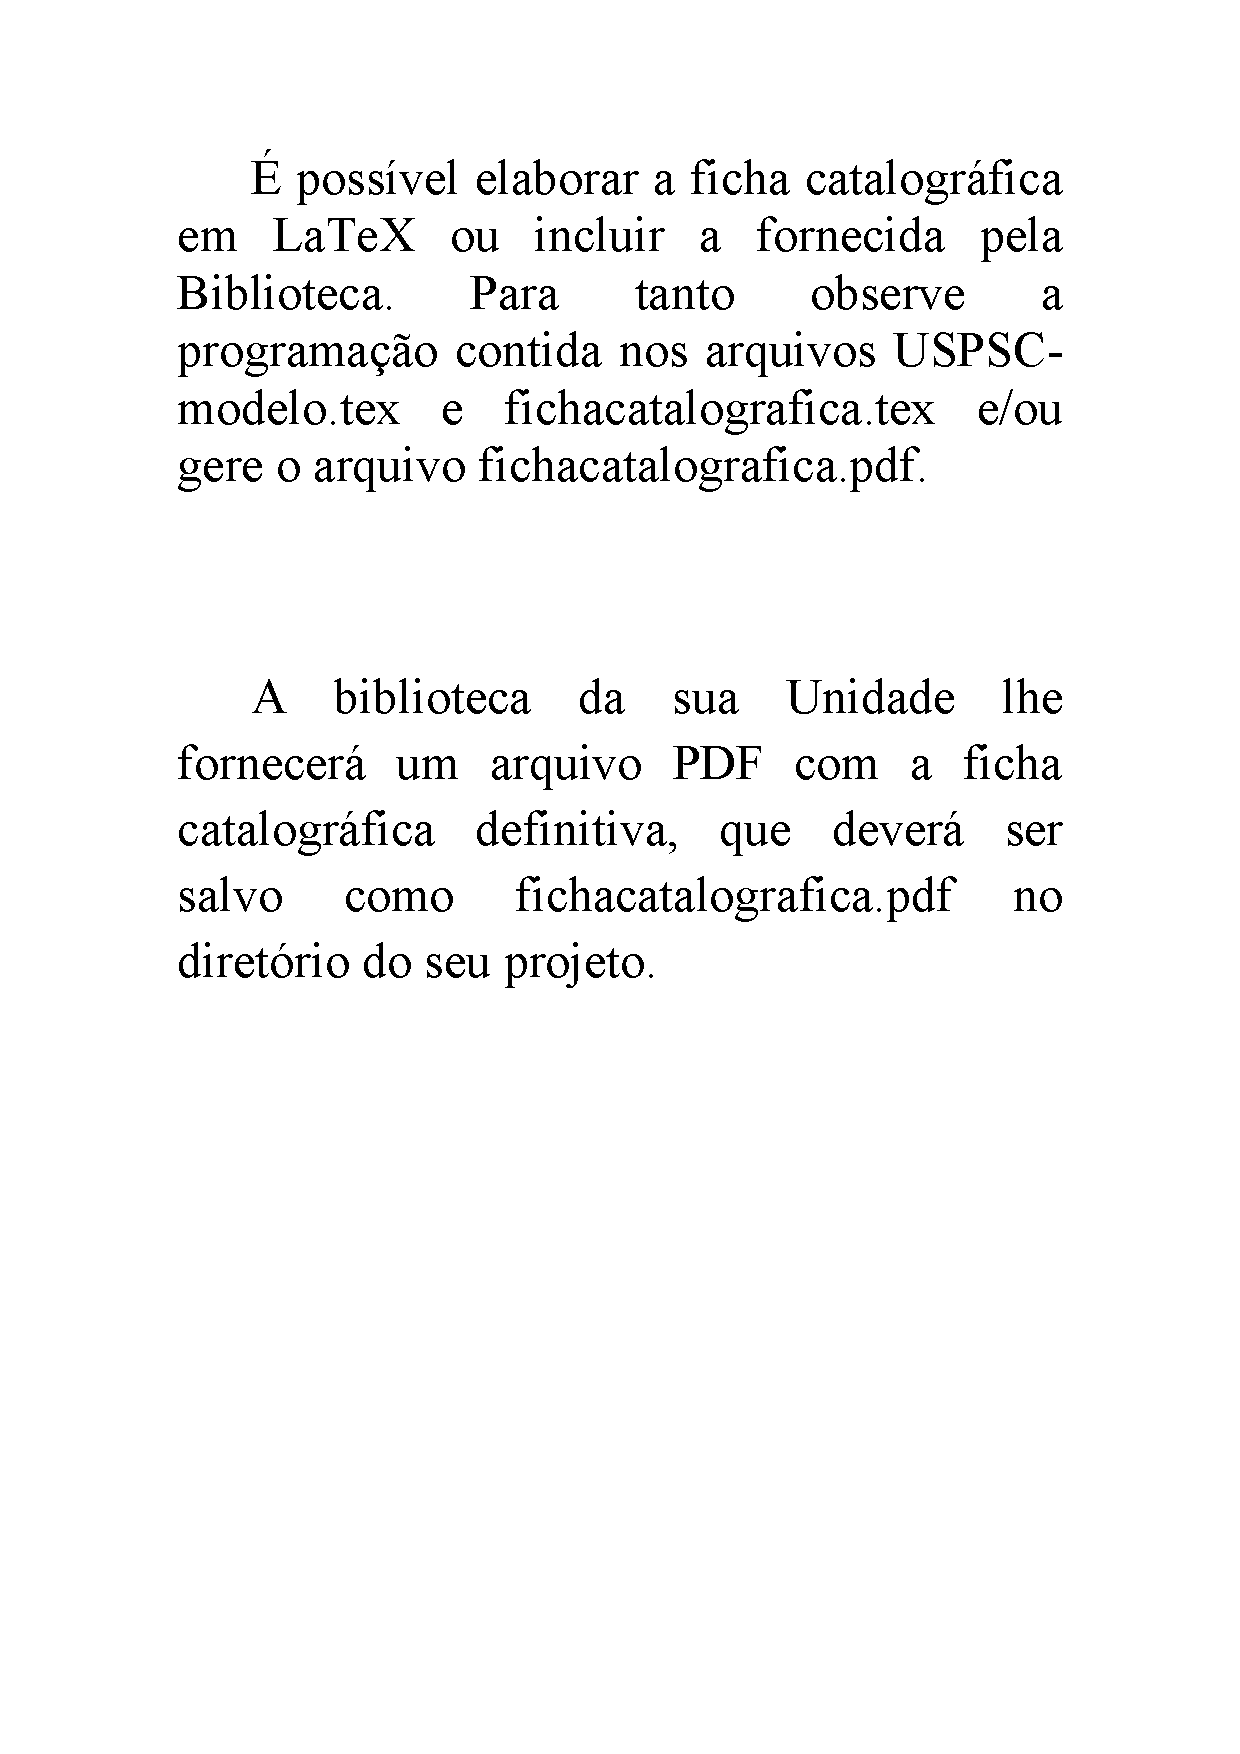
\includepdf{USPSC-TA-PreTextual/USPSC-fichacatalografica.pdf}

% Se você optar por elaborar a ficha catalográfica, deverá 
% incluir uma % antes da linha % antes
% do comando %% USPSC-fichacatalografica.tex
% ---
% Inserir a ficha bibliografica
% ---
% Isto é um exemplo de Ficha Catalográfica, ou ``Dados internacionais de
% catalogação-na-publicação''. Você pode utilizar este modelo como referência. 
% Porém, provavelmente a biblioteca da sua universidade lhe fornecerá um PDF
% com a ficha catalográfica definitiva após a defesa do trabalho. Quando estiver
% com o documento, salve-o como PDF no diretório do seu projeto e substitua todo
% o conteúdo de implementação deste arquivo pelo comando abaixo:
%
\begin{fichacatalografica}
	\hspace{-1.4cm}
	\imprimirnotaautorizacao \\ \\
	%\sffamily
	\vspace*{\fill}					% Posição vertical
\begin{center}					% Minipage Centralizado
  \imprimirnotabib \\
  \begin{table}[htb]
	\scriptsize
	\centering	
	\begin{tabular}{|p{0.9cm} p{8.7cm}|}
		\hline
	      & \\
		  &	  \imprimirautorficha     \\
		
		 \imprimircutter & 
							\hspace{0.4cm}\imprimirtitulo~  / ~\imprimirautor~ ;  ~\imprimirorientadorcorpoficha. -- 	\imprimirlocal, \imprimirdata.   \\
		
		  &  % Para incluir nota referente à versão corrigida no corpo da ficha,
			  % incluir % no início da linha acima e tirar a % do início da linha abaixo
			  %	\hspace{0.4cm} \imprimirtitulo~  / ~\imprimirautor~ ; ~\imprimirorientadorcorpoficha~- ~\imprimirnotafolharosto. -- \imprimirlocal, \imprimirdata.  \\
		
			\hspace{0.4cm}\pageref{LastPage} p. : il. (algumas color.) ; 30 cm.\\ 
		  & \\
		  & 
		    \hspace{0.4cm}\imprimirnotaficha ~--~ 
						  \imprimirunidademin, 
						  \imprimiruniversidademin, 
		                  \imprimirdata. \\ 
		  & \\                 
		   % Para incluir nota referente à versão corrigida em notas,
		    % incluir uma % no início da linha acima e	
		    % tirar a % do início da linha abaixo
		    % & \hspace{0.4cm}\imprimirnotafolharosto \\ 
		  & \\ 
		  & \hspace{0.4cm}1. Segurança Cibernética. 2. Vulnerabilidades. 3. OPC UA. 4. Indústria 4.0. 
              I. \imprimirorientadorficha. 
		   II. Título. \\
	
		     %Se houver co-orientador, inclua % antes da linha (antes de II. Título.) 
		     %          e tire a % antes do comando abaixo 
		     %III. Título. \\   
		  \hline
	\end{tabular}
  \end{table}
\end{center}
\end{fichacatalografica}
% ---

 
% e retirar o % do comando abaixo
% %% USPSC-fichacatalografica.tex
% ---
% Inserir a ficha bibliografica
% ---
% Isto é um exemplo de Ficha Catalográfica, ou ``Dados internacionais de
% catalogação-na-publicação''. Você pode utilizar este modelo como referência. 
% Porém, provavelmente a biblioteca da sua universidade lhe fornecerá um PDF
% com a ficha catalográfica definitiva após a defesa do trabalho. Quando estiver
% com o documento, salve-o como PDF no diretório do seu projeto e substitua todo
% o conteúdo de implementação deste arquivo pelo comando abaixo:
%
\begin{fichacatalografica}
	\hspace{-1.4cm}
	\imprimirnotaautorizacao \\ \\
	%\sffamily
	\vspace*{\fill}					% Posição vertical
\begin{center}					% Minipage Centralizado
  \imprimirnotabib \\
  \begin{table}[htb]
	\scriptsize
	\centering	
	\begin{tabular}{|p{0.9cm} p{8.7cm}|}
		\hline
	      & \\
		  &	  \imprimirautorficha     \\
		
		 \imprimircutter & 
							\hspace{0.4cm}\imprimirtitulo~  / ~\imprimirautor~ ;  ~\imprimirorientadorcorpoficha. -- 	\imprimirlocal, \imprimirdata.   \\
		
		  &  % Para incluir nota referente à versão corrigida no corpo da ficha,
			  % incluir % no início da linha acima e tirar a % do início da linha abaixo
			  %	\hspace{0.4cm} \imprimirtitulo~  / ~\imprimirautor~ ; ~\imprimirorientadorcorpoficha~- ~\imprimirnotafolharosto. -- \imprimirlocal, \imprimirdata.  \\
		
			\hspace{0.4cm}\pageref{LastPage} p. : il. (algumas color.) ; 30 cm.\\ 
		  & \\
		  & 
		    \hspace{0.4cm}\imprimirnotaficha ~--~ 
						  \imprimirunidademin, 
						  \imprimiruniversidademin, 
		                  \imprimirdata. \\ 
		  & \\                 
		   % Para incluir nota referente à versão corrigida em notas,
		    % incluir uma % no início da linha acima e	
		    % tirar a % do início da linha abaixo
		    % & \hspace{0.4cm}\imprimirnotafolharosto \\ 
		  & \\ 
		  & \hspace{0.4cm}1. Segurança Cibernética. 2. Vulnerabilidades. 3. OPC UA. 4. Indústria 4.0. 
              I. \imprimirorientadorficha. 
		   II. Título. \\
	
		     %Se houver co-orientador, inclua % antes da linha (antes de II. Título.) 
		     %          e tire a % antes do comando abaixo 
		     %III. Título. \\   
		  \hline
	\end{tabular}
  \end{table}
\end{center}
\end{fichacatalografica}
% ---


% As informações que compõem a ficha catalográfica estão 
% definidas no arquivo USPSC-pre-textual-UUUU.tex
% ---

% ---
% Folha de rosto adicional
% Para imprimir a folha de rosto adicional, exigida por algumas Unidades, a exemplo do ICMC,
% retire a % antes do comando abaixo

%\imprimirfolhaderostoadic

% ---
% ---
% Inserir errata
% ---

% %% USPSC-Errata.tex
\begin{errata}
	%\OnehalfSpacing 			
	A errata é um elemento opcional, que consiste de uma lista de erros da obra, precedidos pelas folhas e linhas onde eles ocorrem e seguidos pelas correções correspondentes. Deve ser inserida logo após a folha de rosto e conter a referência do trabalho para facilitar sua identificação, conforme a ABNT NBR 14724 \cite{turcato2020}.
	
	Modelo de Errata:
		
	\begin{flushleft} 
			\setlength{\absparsep}{0pt} % ajusta o espaçamento da referência	
			\SingleSpacing 
			\imprimirautorabr~ ~\textbf{\imprimirtituloresumo}.	\imprimirdata. \pageref{LastPage}p. 
			%Substitua p. por f. quando utilizar oneside em \documentclass
			%\pageref{LastPage}f.
			\imprimirtipotrabalho~-~\imprimirinstituicao, \imprimirlocal, \imprimirdata. 
 	\end{flushleft}
\vspace{\onelineskip}
\OnehalfSpacing 
\center
\textbf{ERRATA}
\vspace{\onelineskip}
\OnehalfSpacing 
\begin{table}[htb]
	\center
	\footnotesize
	\begin{tabular}{p{2cm} p{2cm} p{4cm} p{4cm} }
		\hline
		\textbf{Folha} & \textbf{Linha}  & \textbf{Onde se lê}  & \textbf{Leia-se}  \\
			\hline
			1 & 10 & auto-conclavo & autoconclavo\\
		\hline
	\end{tabular}
\end{table}
\end{errata}
% ---

% ---

% ---
% Inserir folha de aprovação
% ---

% A Folha de aprovação é um elemento obrigatório da NBR 4724/2011 (seção 4.2.1.3). 
% Após a defesa/aprovação do trabalho, gere o arquivo folhadeaprovacao.pdf da página assinada pela banca 
% e iclua o arquivo utilizando o comando abaixo:
%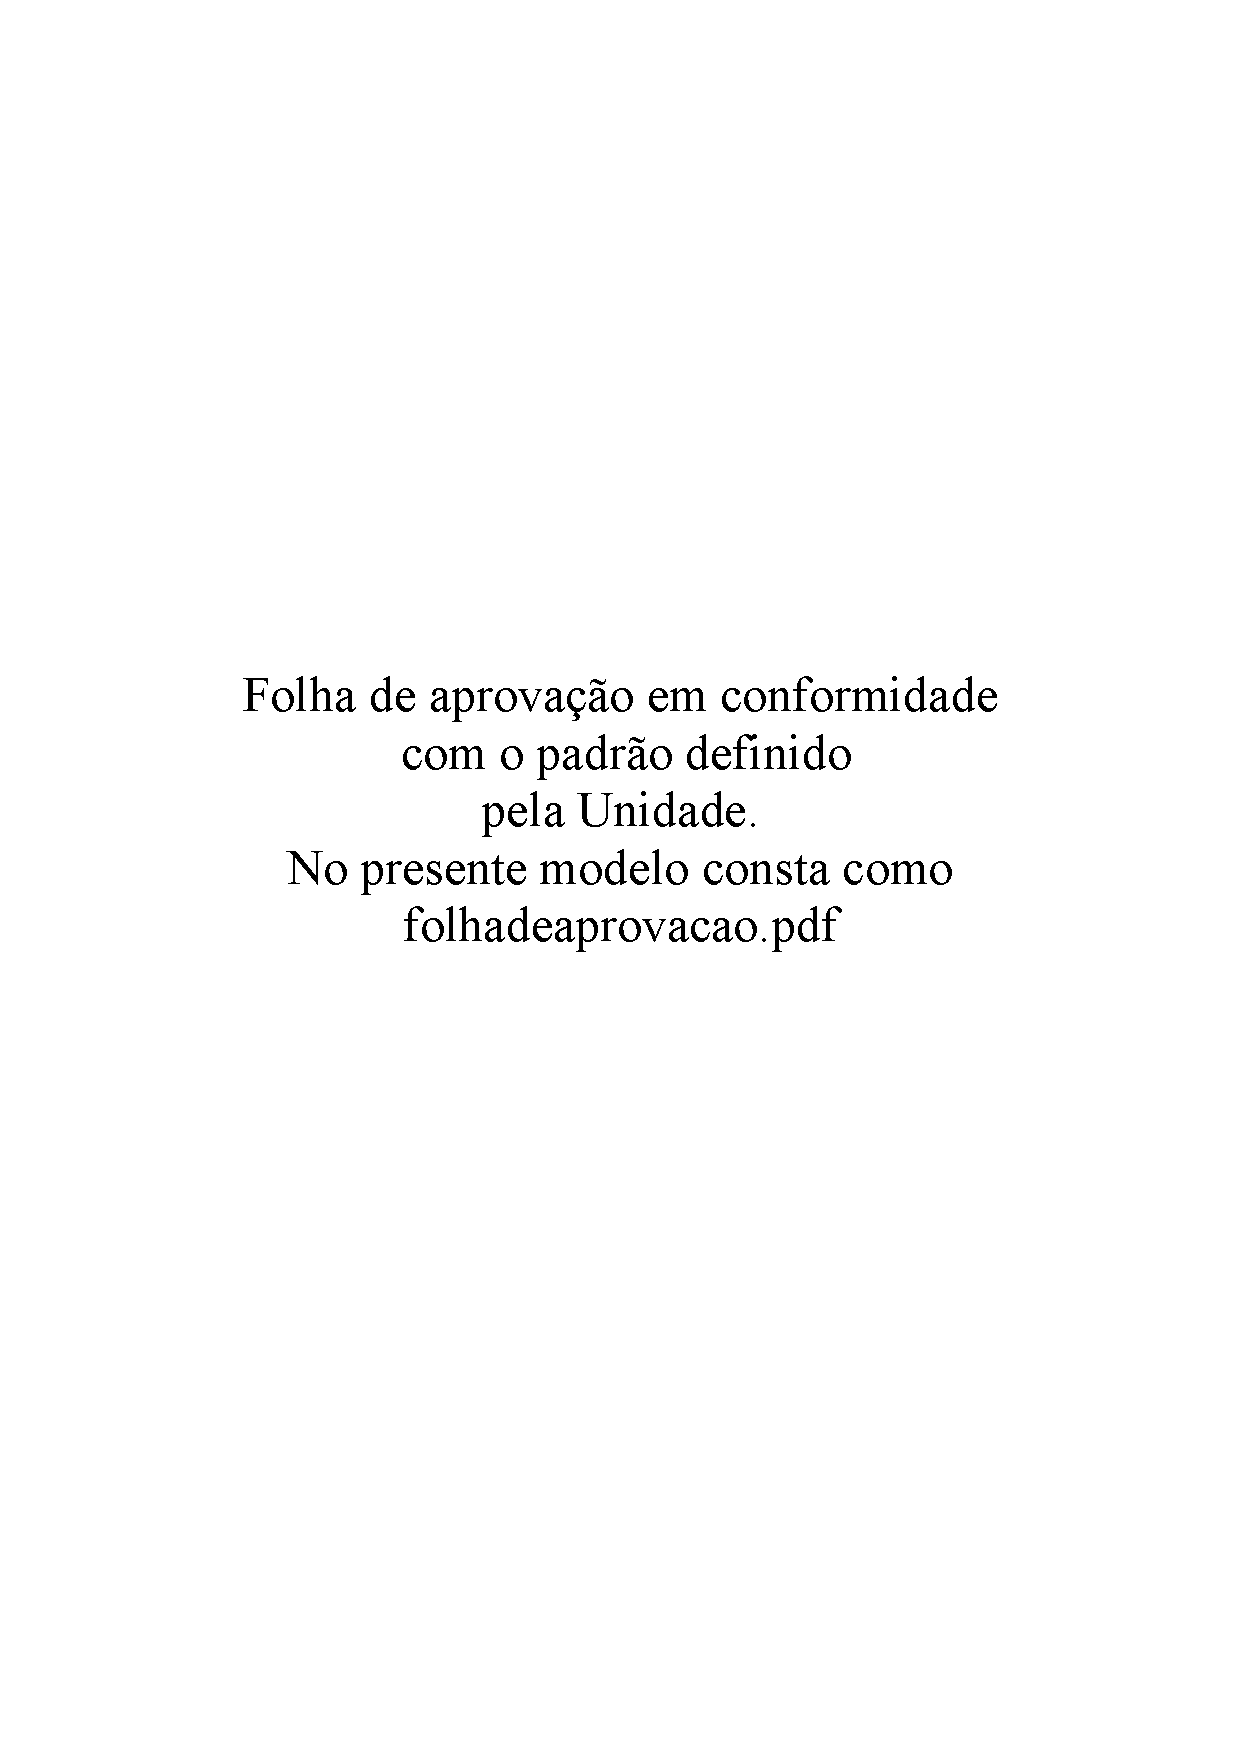
\includepdf{USPSC-TA-PreTextual/USPSC-folhadeaprovacao.pdf}
% Alternativa para a Folha de Aprovação:
% Se for a sua opção elaborar uma folha de aprovação, insira uma % antes do comando acima que inclui o arquivo folhadeaprovacao.pdf,
% tire o % do comando abaixo e altere o arquivo folhadeaprovacao.tex conforme suas necessidades
%% USPSC-folhadeaprovacao.tex
% Alternativa para a Folha de Aprovação 
% Se esta for a sua opção, exclua inclusão feita acima do arquivo folhadeaprovacao.pdf
%
\begin{folhadeaprovacao}
  \begin{center}
       {\ABNTEXchapterfont\bfseries\large\imprimirautor}
	 \vspace*{2cm}
   
    \begin{center}
      \ABNTEXchapterfont\bfseries\Large\imprimirtitulo
    \end{center}
		\vspace*{2cm}
		\hspace{.45\textwidth}
    \begin{minipage}{.5\textwidth}
        \imprimirpreambulo
    \end{minipage}
		\vspace*{2cm}
    %\vspace*{\fill}
	\end{center}

  \begin{center}
	  {\ABNTEXchapterfont\bfseries\large\ {Data de defesa: 20 de fevereiro de 2024} \\}
		\vspace*{\fill}
	  {\ABNTEXchapterfont\bfseries\large\ {Comiss\~ao Julgadora:} \\}
		%Trabalho aprovado. \imprimirlocal, 2 de outubro de 2015:
		
		%\assinatura{\textbf{\imprimirorientador} \\ Orientador} 
		\assinatura{\textbf{\imprimirorientador} \\}
    % Se for ORIENTADOR, inclua % no início do comando abaixo e tire a % do próximo comando 
		\renewcommand{\orientadorname}{Orientador}
		%\renewcommand{\orientadorname}{Orientador}

		\imprimirorientadorRotulo
		\par
		\assinatura{\textbf{Prof. Dr. André Luís Dias} \\ Convidado 1}
	
		\assinatura{\textbf{Professor} \\ Convidado 2}
		%\assinatura{\textbf{Professor} \\ Convidado 3}
		%\assinatura{\textbf{Professor} \\ Convidado 4}
		%\begin{center}
		\vspace*{\fill}
   	{\ABNTEXchapterfont\bfseries\large\imprimirlocal}
    \par
    {\ABNTEXchapterfont\bfseries\large\imprimirdata}
\end{center}
\end{folhadeaprovacao}
% ---

\includepdf{USPSC-TA-PreTextual/USPSC-PaginaEmBranco.pdf}

% ---
% Dedicatória
% ---
%% USPSC-Dedicatoria.tex
\begin{dedicatoria}
    \vspace*{\fill}
    \centering
    \noindent
    \textit{ Dedico este trabalho à minha esposa Carolina e à minha filha Catarina, minhas \\
    fontes de inspiração e força. O apoio incondicional, o amor e o carinho que recebo de vocês \\ 
    são os pilares fundamentais que me sustentam diante das adversidades da vida.\\
    Muito obrigado!} \vspace*{\fill}

\end{dedicatoria}
% ---
% ---

% ---
% Agradecimentos
% ---
%% USPSC-Agradecimentos.tex
\begin{agradecimentos}

    Diante do desafio complexo enfrentado no desenvolvimento dessa dissertação de mestrado, envolvendo os mais variados obstáculos pessoais e profissionais, encontro-me, ao término dessa jornada, diante de uma oportunidade de expressar os sentimentos de gratidão que emergem dentro de mim.

    % Primeiramente, agradeço a Deus, todo-poderoso, por derramar infinitas bençãos em minha vida, confiando e não desistindo desse simples pecador; sem Ele, nada seria e não estaria vivendo momentos tão incríveis ao lado das melhores companhias, aqui prestigiadas. À mãe Maria, agraciada, que tantas vezes guiou meus passos para que conseguisse realizar os objetivos durante esses cinco anos de graduação.
    
    % Em especial à minha família, meu alicerce aqui na Terra. Aos pais Alessandra e Daniel, sempre me orientando para um bom caminho através do exemplo e do amor. Serei eternamente grato a vocês pelas inúmeras privações e sacrifícios que passaram para que eu pudesse ser a pessoa que sou hoje e estar aqui finalizando minha graduação. Ao meu irmão Nícolas, companheiro de todas as situações que essa vida proporciona e que me ensina a ser melhor apenas com seu sorriso e coração, através da sua bondade que contagia. E ao restante da família, obrigado por serem os anjos enviados por Deus para me acolher, auxiliar e instruir em todos os momentos.

    % À minha noiva Carolina, meu grande amor, agradeço infinitamente pelo incentivo e motivação para que eu concluísse esta etapa; mas principalmente, pelo amor, elogios e críticas que me direcionam no caminho da sabedoria. A sua sensatez e lealdade são essenciais para meu desenvolvimento.

    % Aos meus amigos de república: Daniel, Felipe, Henrique, Juliano, Weslley e aos demais colegas da turma por toda descontração, parceria e fidelidade durante todos esses anos.

    % Ao professor e amigo Dr. André Luís Dias, pela oportunidade de sua orientação neste trabalho, sou grato por todo apoio, auxílio e conselhos concebidos durante minha graduação.

    % Honro o fechamento deste ciclo agradecendo também a todos os meus professores(as) por serem uma constante fonte de motivação; por toda a amizade e carinho ao longo dessa caminhada.
	
\end{agradecimentos}
% ---

% ---
% Epígrafe
% ---
%% USPSC-Epigrafe.tex
\begin{epigrafe}
    \vspace*{\fill}
	\begin{flushright}
		\textit{``The only way to do great work is to love what you do. \\
                    If you haven’t found it yet, keep looking. Don’t settle. \\ 
                    As with all matters of the heart, you’ll know when you find it.''\\
		Steve Jobs}
	\end{flushright}
\end{epigrafe}
% ---
% ---

% A T E N Ç Ã O
% Se o idioma do texto for em inglês, o abstract deve preceder o resumo
% resumo em português
%
% Resumo
% ---
%% USPSC-Resumo.tex
\setlength{\absparsep}{18pt} % ajusta o espaçamento dos parágrafos do resumo		
\begin{resumo}
	\begin{flushleft} 
			\setlength{\absparsep}{0pt} % ajusta o espaçamento da referência	
			\SingleSpacing 
			\imprimirautorabr~~\textbf{\imprimirtituloresumo}.	\imprimirdata. \pageref{LastPage}p. 
			%Substitua p. por f. quando utilizar oneside em \documentclass
			%\pageref{LastPage}f.
			\imprimirtipotrabalho~-~\imprimirinstituicao, \imprimirlocal, \imprimirdata. 
 	\end{flushleft}
\OnehalfSpacing

O crescimento avançado da transformação digital, uma consequência direta da quarta revolução industrial, tem impulsionado de forma substancial a interconexão entre dispositivos e sistemas, introduzindo desafios significativos no âmbito da proteção de dados e sistemas críticos. A mudança de paradigma que caracteriza a convergência entre as tecnologias de informação e operacional requer uma análise criteriosa, sobretudo na indústria, cujos sistemas de automação e controle desempenham um papel central. Neste contexto, o protocolo OPC UA emerge como uma peça-chave ao permitir a transferência segura de informações entre uma variedade de dispositivos e sistemas. Não obstante, considerando a constante evolução das ameaças cibernéticas, é imprescindível adotar uma abordagem proativa na identificação e mitigação de vulnerabilidades. Esse estudo apresenta uma análise de vulnerabilidades em redes OPC UA, por meio da implementação de uma bancada experimental especialmente concebida para simular ataques cibernéticos. Os resultados da análise realizada na execução dos ataques de \textit{sniffing} de pacotes, MITM e DoS, reforçam a resiliência destas redes e, simultaneamente, contribuem para o contínuo aprimoramento do protocolo em questão. Assim, a pesquisa desempenha um papel crucial ao proporcionar percepções valiosas e abordagens concretas para a proteção de IACSs em um ambiente caracterizado por uma rápida evolução tecnológica.
 
 \textbf{Palavras-chave}: Segurança Cibernética. OPC UA. Vulnerabilidades. Ataques. IACS.
\end{resumo}
% ---

% Abstract
% ---
%% USPSC-Abstract.tex
%\autor{Silva, M. J.}
\begin{resumo}[Abstract]
 \begin{otherlanguage*}{english}
	\begin{flushleft} 
		\setlength{\absparsep}{0pt} % ajusta o espaçamento dos parágrafos do resumo		
 		\SingleSpacing  		\imprimirautorabr~~\textbf{\imprimirtitleabstract}.	\imprimirdata.  \pageref{LastPage}p. 
		%Substitua p. por f. quando utilizar oneside em \documentclass
		%\pageref{LastPage}f.
		\imprimirtipotrabalhoabs~-~\imprimirinstituicao, \imprimirlocal, 	\imprimirdata. 
 	\end{flushleft}
	\OnehalfSpacing 
   The rapid growth of digital transformation, a direct consequence of the Fourth Industrial Revolution, has substantially driven the interconnection of devices and systems, introducing significant challenges in the realm of data protection and critical system security. The paradigm shift characterizing the convergence of information and operational technologies demands careful scrutiny, particularly within the industrial sector, where automation and control systems play a central role. In this context, the OPC UA protocol emerges as a pivotal component, enabling secure information transfer among a variety of devices and systems. Nevertheless, given the constant evolution of cyber threats, it is imperative to adopt a proactive approach to identify and mitigate vulnerabilities. This study presents a meticulous analysis of vulnerabilities in networks OPC UA, implemented through a specially designed experimental setup to simulate cyberattacks. The results of the analysis, conducted through packet sniffing, Man in the Middle (MITM), and Denial of Service (DoS) attacks, reaffirm the resilience of these networks while simultaneously contributing to the ongoing improvement of the protocol in question. Thus, this research plays a crucial role in providing valuable insights and concrete approaches for safeguarding Industrial Automation and Control Systems (IACSs) in an environment characterized by rapid technological evolution.

   \vspace{\onelineskip}
 
   \noindent 
   \textbf{Keywords}: Cybersecurity. OPC UA. Vulnerabilities. Attack. IACS.
 \end{otherlanguage*}
\end{resumo}

% ---

% ---
% inserir lista de figurass
% ---
\pdfbookmark[0]{\listfigurename}{lof}
\listoffigures*
\cleardoublepage
% ---

% ---
% inserir lista de tabelas
% ---
\pdfbookmark[0]{\listtablename}{lot}
\listoftables*
\cleardoublepage
% ---

% ---
% inserir lista de quadros
% ---
\pdfbookmark[0]{\listofquadroname}{loq}
\listofquadro*
\cleardoublepage
% ---

% ---
% inserir lista de abreviaturas e siglas
% ---
% USPSC-AbreviaturasSiglas.tex
\begin{siglas}
    \item[AI] \textit{Artificial Intelligence}
    \item[ARP] \textit{Address Resolution Protocol}
    \item[APT] \textit{Advanced Persistent Threat}
    \item[CLP] Controlador Lógico Programável
    \item[CoAP] \textit{Constrained Application Protocol}
    \item[DCS] \textit{Distributed Control System}
    \item[IHM] Interface Homem-Máquina
    \item[IACS] \textit{Industrial Automation and Control Systems}
    \item[SDI] Sistema de Detecção de Intrusão
    \item[IIoT] \textit{Industrial Internet of Things}
    \item[IoT] \textit{Internet of Things}
    \item[TI] Tecnologia da Informação
    \item[LGPD] Lei Geral de Proteção de Dados
    \item[MAC] \textit{Media Access Control}
    \item[MQTT] \textit{Message Queuing Telemetry Transport}
    \item[O-PAS] \textit{Open Process Automation™ Standards}
    \item[OPAF] \textit{Open Process Automation™ Forum}
    \item[OPC UA] \textit{Open Platform Communications – Unified Architecture}
    \item[OSI] \textit{Open Systems Interconnection}
    \item[TO] Tecnologia Operacional
    \item[SCADA] \textit{Supervisory Control and Data Acquisition}
    \item[SOA] \textit{Service Oriented Architecture}
    \item[TSN] \textit{Time Sensitive Networking}
    \item[UTM] \textit{Unified Threat Management}
    \item[XML] \textit{Extensible Markup Language}
\end{siglas}

% ---

% ---
% inserir lista de símbolos
% ---
% USPSC-Simbolos.tex
\begin{simbolos}
  \item[$ \Gamma $] Letra grega Gama
  \item[$ \Lambda $] Lambda
  \item[$ \zeta $] Letra grega minúscula zeta
  \item[$ \in $] Pertence
\end{simbolos}
% ---
% ---
% inserir o sumario
% ---
\pdfbookmark[0]{\contentsname}{toc}
\tableofcontents*
\cleardoublepage
% ---
% ----------------------------------------------------------
% ELEMENTOS TEXTUAIS
% ----------------------------------------------------------
\textual
% Os capítulos são inseridos como arquivos externos 

% Capítulos
%% USPSC-Introducao.tex

% ----------------------------------------------------------
% Introdução (exemplo de capítulo sem numeração, mas presente no Sumário)
% ----------------------------------------------------------

\chapter[Introdução]{Introdução} \label{cap:introducao}

    A tecnologia atual tem impulsionado significativamente o nível da troca de informações nas mais diversas áreas do mundo, provocando mudanças substanciais em nossa forma de viver, enfrentar desafios e relacionar. Especialmente no setor industrial, essa transformação exige uma gestão de dados que esteja intrinsecamente vinculada ao aprimoramento da eficiência e produtividade.
    
    Esse movimento de transformação digital ficou conhecido como a quarta revolução industrial, ou \index{Indústria 4.0}Indústria 4.0, caracterizando-se pela integração de tecnologias avançadas como a internet das coisas industrial (\index{IIoT}IIoT, do inglês \textit{Industrial Internet of Things}), \index{Inteligência Artificial}Inteligência Artificial (AI, do inglês \textit{Artificial Intelligence}) e processamento de dados em larga escala (também denominados como \textit{Big Data} e \textit{Data Warehousings}).
    
    À medida que o número de dispositivos interconectados e a quantidade de dados gerados por esses aumentam exponencialmente, a necessidade de estratégias robustas de \index{Segurança Cibernética}segurança cibernética torna-se igualmente crucial, a fim de garantir a proteção da ampla exposição dessas informações às atividades maliciosas e \index{Ataque Cibernético}ataques cibernéticos. De acordo com \citeonline{wef2022}:
    
    \begin{citacao}
        Conforme a sociedade continua a migrar para o mundo digital, a ameaça do crime cibernético se torna grande, custando rotineiramente às organizações dezenas – até mesmo centenas – de milhões de dólares. Os custos não são apenas financeiros: infraestrutura crítica, coesão social e bem-estar mental também estão em risco.
    \end{citacao}

    As redes de comunicação industriais não estão imunes aos desafios que surgem com o aumento exponencial na troca de informações. A interconexão de sistemas em um ambiente industrial requer uma abordagem especializada para enfrentar as crescentes \index{Ameaça Cibernética}ameaças cibernéticas que acompanham essa revolução tecnológica. Portanto, é imperativo que as empresas que operam nesse setor invistam e se desenvolvam em duas áreas de tecnologia fundamentais: da informação (\index{Tecnologia da Informação}TI) --  que desempenha um papel crucial na gestão abrangente da informação -- e operacional (\index{Tecnologia Operacional}TO) -- que abrange os Sistemas de Automação e Controle Industrial (\index{IACS}IACS, do inglês \textit{Industrial Automation and Control Systems}) --, a fim de fortalecer os sistemas de defesas existentes ou desenvolver novas metodologias de defesa.
    
    Até muito recentemente, essas duas áreas de tecnologia (\index{Tecnologia da Informação}TI e \index{Tecnologia Operacional}TO) eram separadas nos níveis técnico e organizacional. A transformação digital supracitada, gerou alguns gatilhos, principalmente no setor industrial, obrigando as organizações a reverem esse paradigma e liderar projetos de convergência entre os dois mundos \cite{yassine2021}. A \index{Convergência TI/TO}convergência TI/TO, conforme definida na literatura \cite{yassine2021,tian2019,garimella2018}, apresenta um desafio significativo para as empresas ao propor a descompartimentação dos dados e a intercambialidade de pilares (\textit{e.g.}, a implementação da computação em nuvem no monitoramento dos processos de \index{IACS}IACS).

    À medida que os processos oriundos dessa convergência se tornam mais precisos e complexos, aumenta-se a relevância da transmissão de dados entre os equipamentos que os controlam. Assim, os protocolos de comunicação emergem como componentes de importância primordial na \index{Convergência TI/TO}convergência TI/TO, pois desempenham um papel fundamental na viabilização da integração eficiente e segura entre esses dois domínios de tecnologia. A interoperabilidade e intercambialidade de um sistema, antes não apresentadas por protocolos industriais proprietários, passam a ser características fundamentais nesse contexto. Desse modo, o protocolo \index{OPC UA}OPC UA (do inglês \textit{Open Platform Communications Unified Architecture}) assume uma posição de destaque e relevância ao estabelecer as bases para a troca de informações contínua, segura e confiável entre dispositivos e sistemas de diferentes origens e finalidades.

    O \index{OPC UA}OPC UA é um protocolo de comunicação amplamente utilizado para aplicações \index{IIoT}IIoT e de automação industrial, no qual foi projetado para fornecer uma camada de comunicação segura e confiável para cenários da \index{Indústria 4.0}Indústria 4.0. Sua construção baseou-se nas seguintes preocupações de segurança, de acordo com \citeonline{pocock2014}: autenticação de usuários/instâncias de aplicativos (software), confidencialidade e integridade ao assinar e criptografar mensagens, disponibilidade por processamento mínimo antes da autenticação e auditabilidade por eventos de auditoria definidos para operações \index{OPC UA}OPC UA. Assim, o OPC UA é amplamente reconhecido como um protocolo seguro, uma vez que incorpora todos os elementos fundamentais para assegurar a comunicação industrial, conforme identificado por  \citeonline{lange2010}. Esse conjunto de medidas de segurança o torna um pilar confiável para a infraestrutura de comunicação em ambientes industriais modernos, cuja integridade e segurança dos dados são de suma importância.

    No entanto, a despeito dessa concepção robusta e meticulosamente direcionada para a segurança que caracteriza o protocolo \index{OPC UA}OPC UA, é imperativo reconhecer a dinamicidade do cenário atual de \index{Segurança Cibernética}segurança cibernética. A evolução tecnológica supramencionada e as táticas adversárias à ética podem resultar no surgimento de novas \index{Ameaça Cibernética}ameaças e \index{Vulnerabilidade}vulnerabilidades a esse protocolo, além da possibilidade de ser significativamente afetado por várias opções de configuração de segurança. Logo, uma postura proativa é crucial para continuar mitigando as \index{Ameaça Cibernética}ameaças emergentes e assegurando a resiliência desse ecossistema industrial. A vigilância e a análise de novas vulnerabilidades são requisitos indispensáveis para o aprimoramento contínuo do \index{OPC UA}OPC UA.

    A análise sistemática de \index{Vulnerabilidade}vulnerabilidades proporciona uma visão crítica das possíveis brechas que possam surgir, permitindo uma abordagem preventiva e corretiva na implementação de soluções adequadas. Ao identificar potenciais pontos de risco no protocolo industrial, é possível adotar medidas de segurança proativas, tais como: atualizações sistêmicas ou estruturais, ajustes de configuração e o estabelecimento de políticas rigorosas. Essa análise, uma vez bem executada, não apenas identifica fragilidades, mas também orienta as estratégias de proteção, concebendo à organização uma posição privilegiada para se comportar de maneira ágil e eficaz contra uma \index{Ameaça Cibernética}ameaça ou \index{Ataque Cibernético}ataque cibernético.

    Neste trabalho, uma análise de \index{Vulnerabilidade}vulnerabilidades em redes industriais \index{OPC UA}OPC UA é realizada com o intuito de fornecer uma abordagem estruturada de avaliação da segurança do protocolo. Adota-se a criação de uma bancada experimental como ambiente industrial de simulação de \index{Ataque Cibernético}ataques cibernéticos. Ao aplicar a abordagem proposta, pretende-se contribuir para o fortalecimento da resiliência dessas redes, assim como colaborar com o desenvolvimento do OPC UA.

    % Neste estudo, propomos um framework para análise de vulnerabilidades no protocolo OPC UA e modelagem de ameaças. Também apresentamos cenários de vulnerabilidades identificadas de acordo com a modelagem de ameaças e sugerimos contramedidas através do processo de prova de conceito para cada cenário configurado.
    
    \section{Motivação e Justificativa} \label{sec:motivacao}

    A investigação de trabalhos na comunidade científica foi utilizada como justificativa da dissertação e motivação ao tópico proposto. Duas buscas principais foram realizadas para que o tema do trabalho fosse definido: a primeira (I) relacionada ao panorama, desafios e oportunidades do protocolo \index{OPC UA}OPC UA no cenário atual, e a segunda (II) com foco no principal gargalo do protocolo observado na pesquisa anterior.
    
    Mediante uma pesquisa sistemática de publicações relacionadas ao protocolo OPC UA na base de dados IEEE Xplore, considerando publicações entre os anos 2018 e 2022, escritas em inglês e aplicando critérios de exclusão, 238 publicações (Artigos, Jornais, Revistas, Atas de Conferências, etc.) foram classificadas em categorias, e seus resultados apresentados e discutidos a fim de fornecer uma visão geral do protocolo e investigar os desafios e oportunidades de sua aplicação em ambientes industriais atuais.

    Inicialmente, utilizaram-se diferentes formas de escrita para o termo \index{OPC UA}`OPC UA' como \textit{Author Keywords} nessa pesquisa inicial, como: `OPC-UA', `OPC:UA' e `OPC \textit{Unified Architecture}', resultando em 263 publicações. A relevância das publicações foi avaliada e, posteriormente, os seguintes critérios de exclusão foram aplicados para eliminar as publicações que não forneciam informações pertinentes:

    \begin{itemize}
        \item O foco principal da publicação não é em redes de comunicação industrial ou em Internet das Coisas (\index{IoT}IoT, do inglês \textit{Internet of Things}), apesar do \index{OPC UA}OPC UA ser utilizado no projeto de pesquisa;
        \item O \index{OPC UA}OPC UA é referenciado na publicação, mas não é um tópico relevante da mesma;
        \item Publicações que se concentram em \textit{marketing} de produtos e não priorizam o \index{OPC UA}OPC UA como protocolo central ou recurso.
    \end{itemize}

    Após a aplicação dos critérios supracitados, um total de 238 publicações foram identificadas e submetidas a uma análise quantitativa. Entre as publicações selecionadas, 227 (95\%) foram publicadas em anais de conferências, enquanto 11 (5\%) foram publicadas em revistas científicas. A distribuição das publicações por jornais e conferências por ano é ilustrada na \autoref{fig:pubPorAno}.

    % {\color{red}
    % A principal revista científica que apresenta artigos relacionados ao OPC UA é `\textit{IEEE Access}', com um total de seis publicações. O \textit{IEEE Access} é uma revista arquivística multidisciplinar, de acesso aberto (OA, do inglês \textit{Open Access}), orientada para aplicações, completamente eletrônica, que apresenta continuamente os resultados de pesquisas ou desenvolvimentos originais em todos os campos de interesse do IEEE \cite{access2023}. 
    
    % Em relação a conferências, simpósios e congressos, a principal conferência para pesquisas relacionadas ao OPC UA foi encontrada na `\textit{IEEE International Conference on Emerging Technologies and Factory Automation (ETFA)}', com um total de 57 publicações. Este número é notável, pois representa 25,1\% de todos os artigos de conferência.
    % } % Fim da cor vermelha

    \begin{figure}[htbp]
        \caption{Número de publicações relacionadas ao OPC UA por ano}
        \label{fig:pubPorAno}
        \begin{center}
            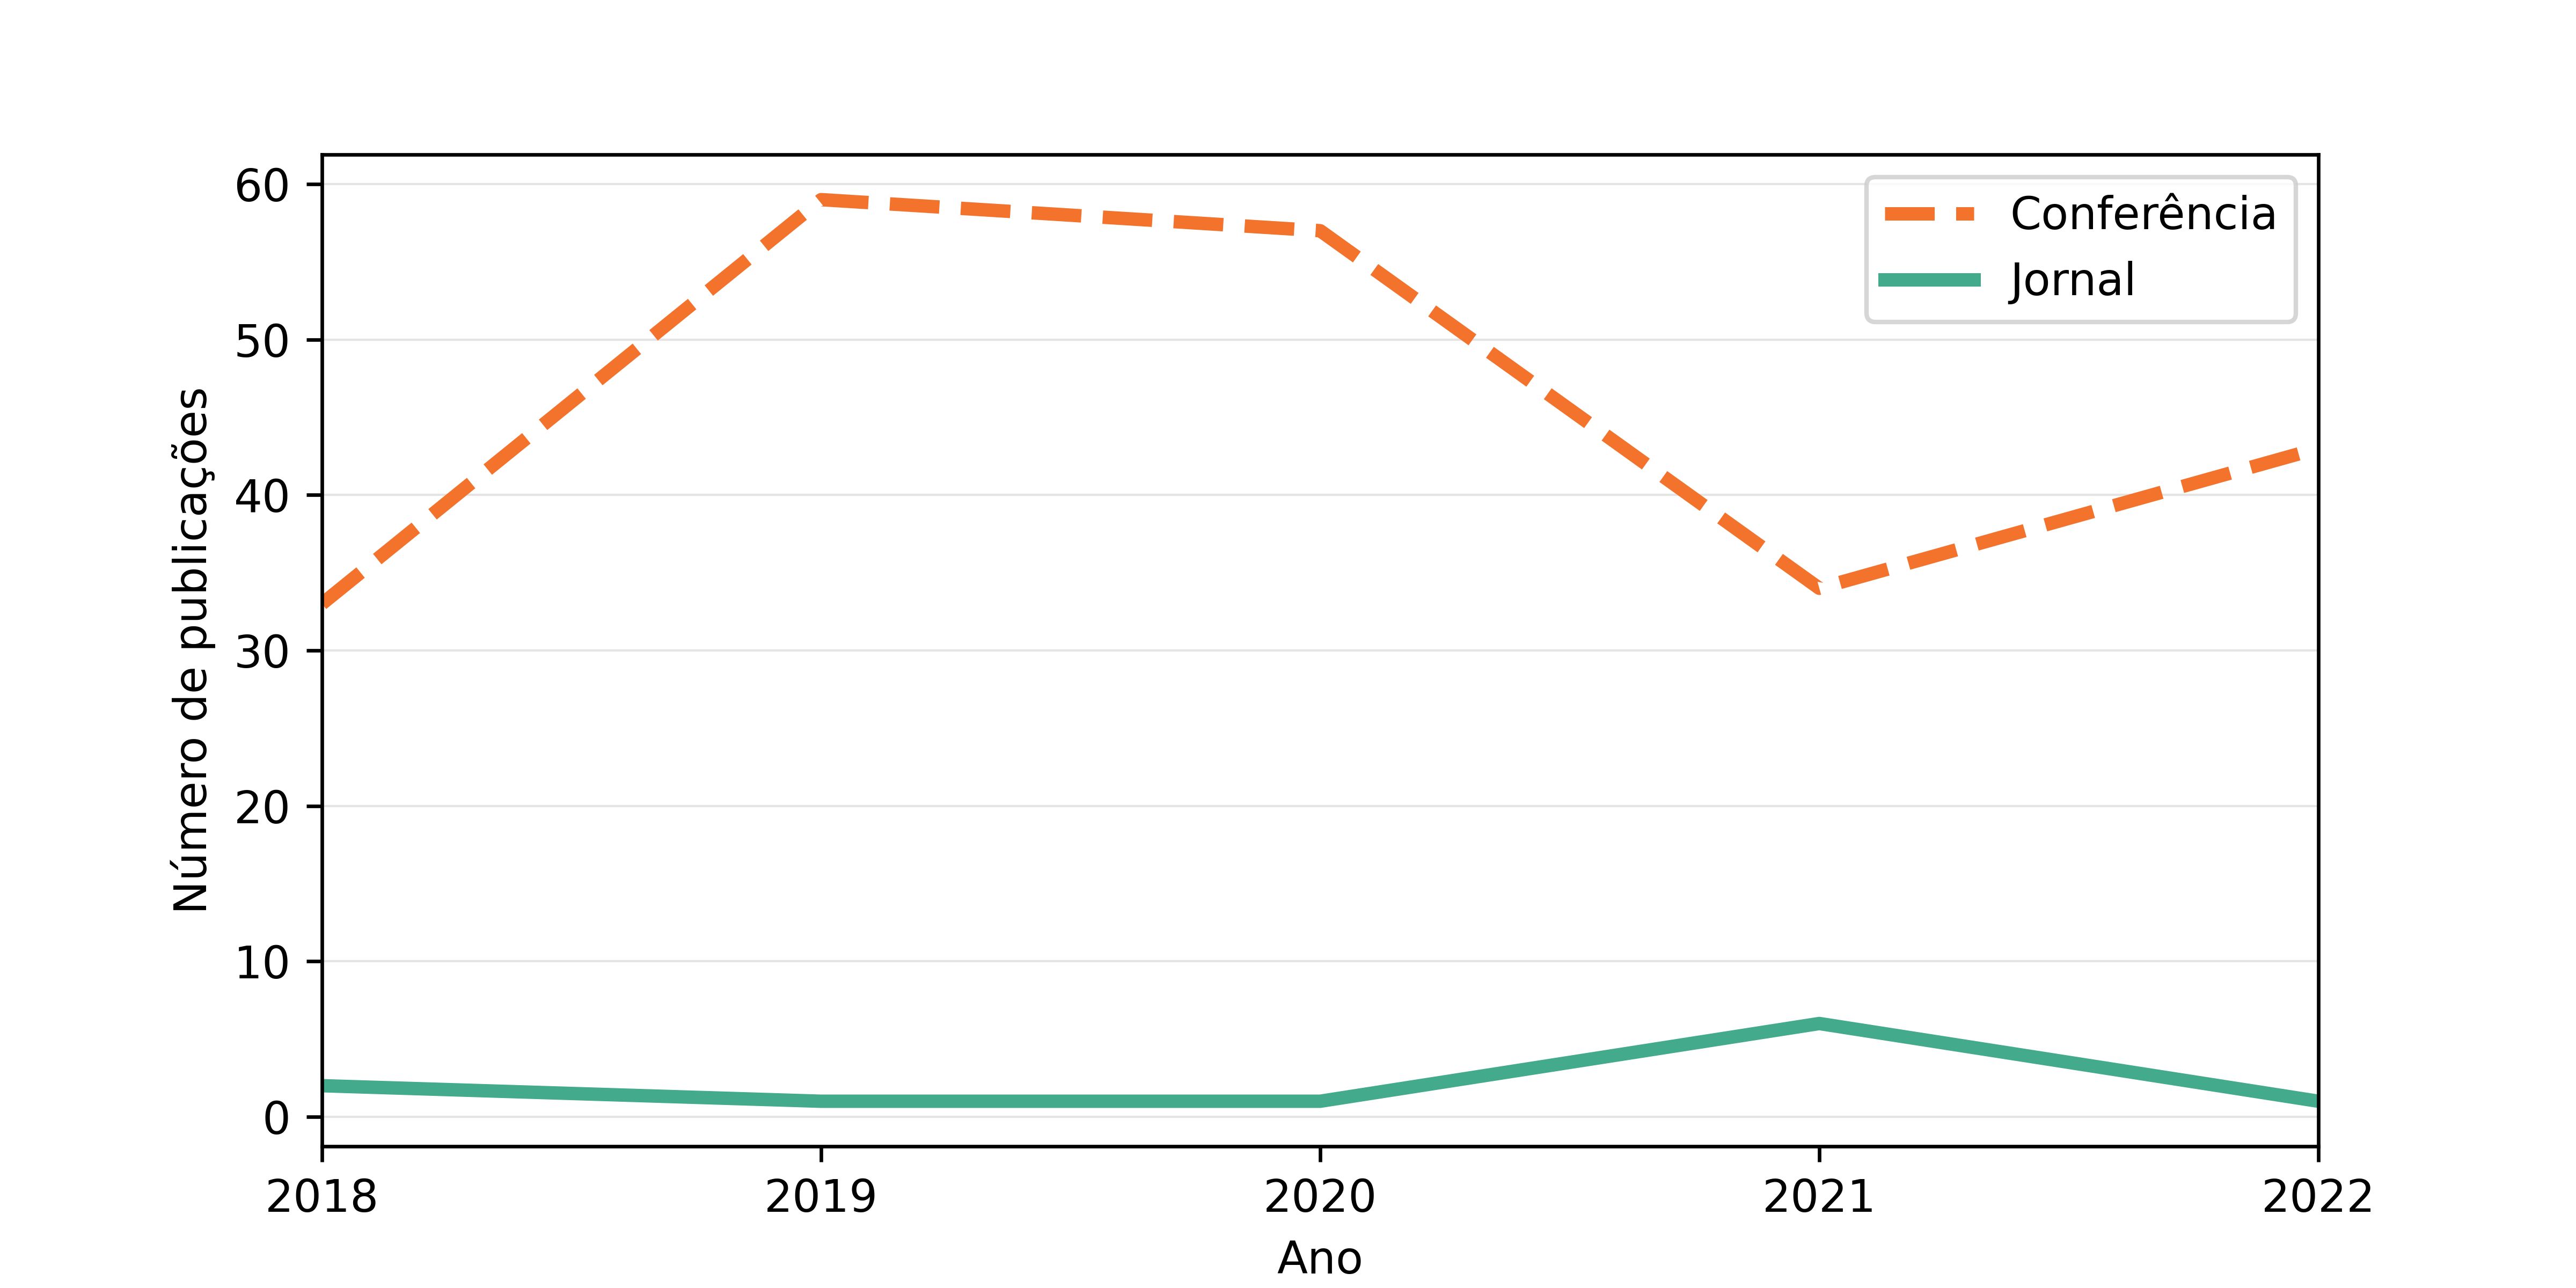
\includegraphics[width=0.7\linewidth]{USPSC-img/pubPerYear.png}
        \end{center}
        \fonte{elaborada pelo autor.}
    \end{figure}

    Após uma leitura e análise cuidadosas, as publicações identificadas foram classificadas nos tópicos sugeridos, conforme apresentado abaixo, seguidos da sua respectiva descrição:

    \begin{itemize}
        \item \underline{Integração e Teoria (TI)}: integração do protocolo com diferentes sistemas, dispositivos e aplicativos por meio de um modelo de dados comum, assim como sobre sua teoria baseada em padrões como IEC 61499 e IEC 62541 e trabalhos de pesquisa existentes;
        \item \underline{Desenvolvimento de Produto (PD)}: criação de novos servidores, clientes, \textit{frameworks} e modelos de informação para expandir a funcionalidade e compatibilidade do \index{OPC UA}OPC UA, fornecendo uma base para novos sistemas e aplicativos industriais;
        \item \underline{Segurança (S)}: enfatiza significativamente a segurança, ao utilizar autenticação, criptografia e controle de acesso para proteger os dados e sistemas industriais contra \index{Ameaça Cibernética}ameaças cibernéticas, ou analisar as implicações de segurança da implementação do protocolo em um sistema;
        \item \underline{Análise de Desempenho (PA)}: análise do desempenho do protocolo, identificação de gargalos e indicação de possíveis melhorias para o desempenho geral do sistema, utilizando medidas como latência, variação de latência, perda de pacotes, taxa de transferência, entre outras métricas para avaliar o comportamento do sistema e verificar a conformidade com os requisitos aplicáveis;
        \item \underline{Comparação de Protocolo (PC)}: comparação com outros protocolos de comunicação industrial e \index{IoT}IoT, principalmente com base em indicadores de desempenho;
        \item \underline{Diagnóstico e Monitoramento (DM)}: oferece recursos de diagnóstico e monitoramento, tais como: monitoramento da saúde do sistema, gerenciamento de alarmes e notificação de eventos, a fim de garantir a disponibilidade do sistema e reduzir o tempo de inatividade;
        \item \underline{Comunicação \textit{Wireless} (W)}: principal característica da rede é a utilização do protocolo \index{OPC UA}OPC UA através de uma comunicação sem fio;
        \item \underline{Outros (O)}: abrange uma ampla gama de áreas de pesquisa relacionadas à tecnologia \index{OPC UA}OPC UA, como modelagem de dados, interoperabilidade semântica, virtualização, computação em nuvem e computação de borda.
    \end{itemize}

    A presente análise tem implicações significativas para identificar lacunas no estado atual da pesquisa na comunidade científica. Um artigo foi desenvolvido, submetido à \textit{IEEE/IAS International Conference on Industry Applications} e aceito para publicação, cuja discussão mais integralizada em relação aos trabalhos atuais para cada categoria é apresentada.
    %\citeonline{} apresenta uma discussão mais integralizada em relação aos trabalhos atuais para cada categoria é apresentada. 
    A literatura existente sobre \index{OPC UA}OPC UA é notavelmente carente de trabalhos que explorem a intersecção entre segurança e comunicação sem fio, o que representa uma lacuna crítica. A \autoref{tab:paperCategory} fornece um resumo abrangente dos tópicos abordados nas publicações identificadas ao longo do período estudado, permitindo uma avaliação sistemática das tendências e padrões na comunidade científica ao longo dos últimos anos.
    
    \begin{table}[htbp]
        \centering
        \caption{Quantidade de publicações por categorias}%
	\label{tab:paperCategory}
        \begin{tabular}{ccccccccc}
            \toprule
            \thead{Ano} & \thead{TI} & \thead{PD} & \thead{S} & \thead{PA} & \thead{PC} & \thead{DM} & \thead{W} & \thead{O} \\
            \toprule
            2018 & 14 & 12 & 4 & 5  & 2  & 2  & 2 & 6 \\
            \midrule
            2019 & 21 & 20 & 6 & 10 & 10 & 10 & 8 & 10 \\
            \midrule
            2020 & 22 & 13 & 6 & 8  & 10 & 13 & 6 & 15 \\
            \midrule
            2021 & 17 & 16 & 4 & 12 & 6  & 3  & 7 & 3 \\
            \midrule
            2022 & 12 & 18 & 5 & 7  & 7  & 5  & 3 & 10 \\
            \bottomrule
            \textbf{Total} & 86 & 79 & 25 & 42 & 35 & 33 & 26 & 44 \\
            \bottomrule
        \end{tabular}
        \fonte{elaborada pelo autor.}%
    \end{table}

    A segurança tem historicamente recebido uma proporção menor de atenção na área de pesquisa. Isso pode ser atribuído ao fato de que o OPC UA foi projetado para incorporar medidas de segurança, incluindo criptografia, autenticação e autorização \cite{lange2010}. Tal abordagem abrangente de segurança, aliada às recomendações e diretrizes de melhores práticas fornecidas pela fundação desenvolvedora, a \textit{OPC Foundation}, contribuiu para uma redução notável na quantidade de pesquisas dedicadas a esse tópico específico.

    % {\color{red}
    % A pesquisa futura pretende aprofundar nas preocupações com a segurança por meio de uma análise quantitativa semelhante à primeira, especificamente nas produções relacionadas à detecção de intrusão ou anomalias neste tipo de rede.
    
    % É importante notar que algumas publicações foram classificadas em mais de uma categoria, indicando a natureza multidisciplinar da pesquisa em torno da tecnologia OPC UA, bem como a predominância de estudos relacionados à integração ao longo das décadas. Uma das razões para isso é o contínuo surgimento de novas tecnologias que complementam a usabilidade do protocolo, introduzindo novas funcionalidades ao sistema geral.

    % A quantidade de estudos sobre o desenvolvimento de produtos é um tópico significativo, o que é refletido pelo número substancial de pesquisas dedicadas à teoria e integração do protocolo com outras tecnologias. Isso é ainda suportado pela projeção feita por \citeonline{industryarc2023}, que estima que o mercado de rede OPC UA experimentará uma taxa de crescimento anual composta (CAGR) de 6,3\% durante o período de previsão de 2021 a 2026, resultando em um tamanho de mercado esperado de US\$ 18,3 bilhões até 2026.
    
    % Embora a análise de desempenho, comparação entre protocolos, diagnóstico e monitoramento sejam áreas importantes de pesquisa, isso não significa que sejam mais significativas do que outros tópicos menos explorados, como segurança e comunicação sem fio. Ainda que o OPC UA tenha sido projetado com uma forte base em segurança e comunicação sem fio, pesquisas adicionais são necessárias para abordar os desafios apresentados pelas tecnologias emergentes, como as redes 5G e TSN, bem como para aprimorar as medidas de cibersegurança. Assim, uma abordagem holística para a pesquisa em OPC UA deve abranger todas essas áreas para garantir a integração perfeita do OPC UA com as tecnologias em evolução da \index{Indústria 4.0}Indústria 4.0.
    
    % As publicações listadas na categoria "Outros (O)", que constituem um número significativo, indicam que o protocolo foi extensivamente estudado em múltiplos domínios dentro da comunidade acadêmica. A literatura sobre este tema tem se concentrado principalmente na aplicação do protocolo em vários contextos.
    % } % Fim da cor vermelha
    
    % \subsection{Pesquisa II}\label{subsec:pesqII}

    As descobertas desse estudo inicial foram significativas ao fornecer uma visão geral e atual do protocolo \index{OPC UA}OPC UA, destacando a necessidade de manter um interesse vigilante na área de segurança, a fim de garantir resiliência do protocolo frente às ameaças constantes a esses sistemas. Assim, uma nova análise quantitativa foi realizada visando o aprofundamento nos trabalhos com esse foco, especificamente naqueles atinentes à segurança cibernética nesse tipo de rede. Para isso, utilizou-se as bases de dados: IEEE Xplore, Web of Science e Scopus.

    Em uma pesquisa inicial, os termos \index{OPC UA}`OPC UA' e `\textit{Security}' foram empregados como \textit{Keywords}, repetindo os mesmos critérios de inclusão relatados na pesquisa anterior. Entretanto, não se aplicou nenhum critério de exclusão. A \autoref{fig:pubAmount} apresenta os resultados separados por ano, de 2013 até o de 2022.

    \begin{figure}[htbp]
        \caption{Quantidade de publicações sobre a segurança em redes OPC UA nos últimos anos}
        \label{fig:pubAmount}
        \begin{center}
            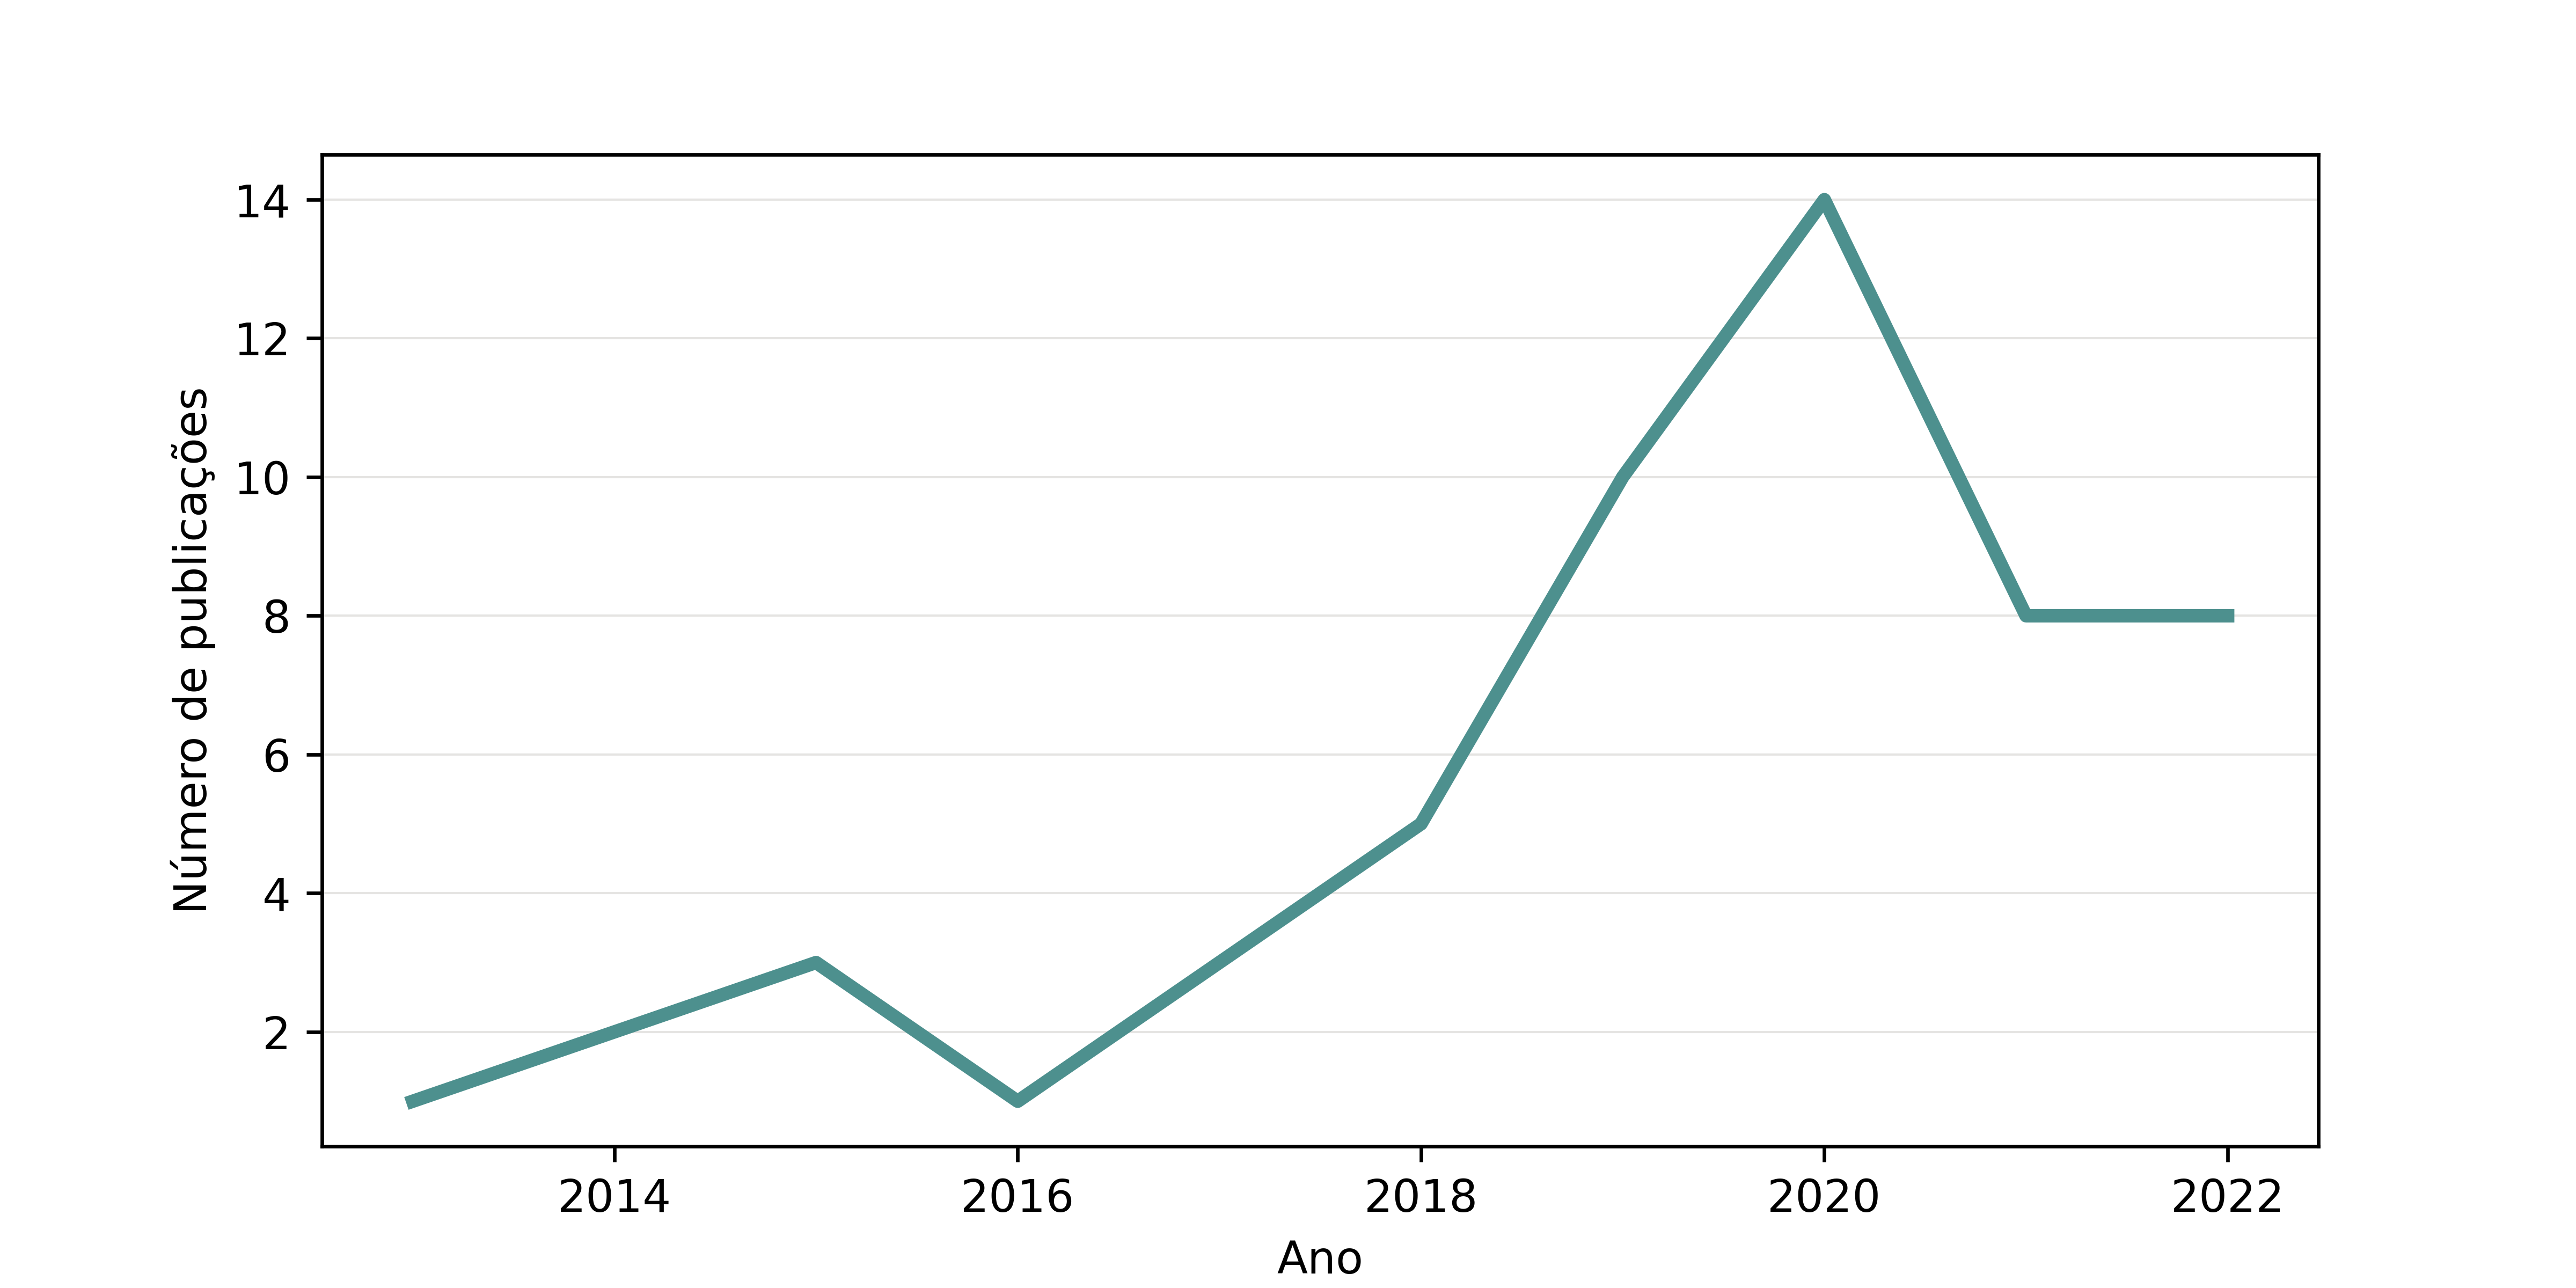
\includegraphics[width=0.7\linewidth]{USPSC-img/pubAmount1.png}
        \end{center}
        \fonte{elaborada pelo autor.}
    \end{figure}

    A análise sobre o panorama das publicações relacionadas à segurança em redes \index{OPC UA}OPC UA ao longo da última década, evidência um notável crescimento na quantidade de trabalhos sobre o tema, indicando um interesse crescente e uma conscientização ampliada acerca dos desafios de segurança envolvendo esse protocolo. No entanto, a partir do ano de 2021, observa-se um fenômeno de diminuição e posterior estagnação nessa produção acadêmica e técnica. Essa tendência decrescente pode derivar de uma combinação de fatores, como: a possibilidade de que muitos aspectos cruciais tenham sido já discutidos e explorados, a influência de outros tópicos emergentes na segurança cibernética, ou até mesmo considerações externas que impactaram a dinâmica da pesquisa e publicação (\textit{e.g.}, pandemia de COVID-19).

    Seguidamente, a estrutura de pesquisa abaixo foi empregada a fim de filtrar aqueles trabalhos relacionados à análise de \index{Vulnerabilidade}vulnerabilidades em redes \index{OPC UA}OPC UA, aplicando como critérios de inclusão: publicações no período de 2013 a 2022, escritas em inglês. Entende-se `TKA' pela junção dos campos \textit{title}, \textit{keywords} e \textit{abstract}. Os resultados estão descritos na \autoref{fig:pubVulAmount}.

    \begin{minted}[
        breaklines,
        %linenos,
        mathescape,
        encoding=utf8,
        framesep=2mm,
        baselinestretch=1.2,
        bgcolor=codeback,
        fontsize=\footnotesize
    ]{vhdl}
("TKA":“OPC UA” OR "TKA":“OPC-UA” OR "TKA":“OPC:UA” OR "TKA":“OPC Unified Automation”) AND ("TKA":“Vulnerabilities” OR "TKA":“Vulnerabilities Analysis” OR "TKA":“Vulnerabilities Assessment”)
    \end{minted}
    
    \begin{figure}[htbp]
        \caption{Quantidade de publicações sobre vulnerabilidades em redes OPC UA nos últimos anos}
        \label{fig:pubVulAmount}
        \begin{center}
            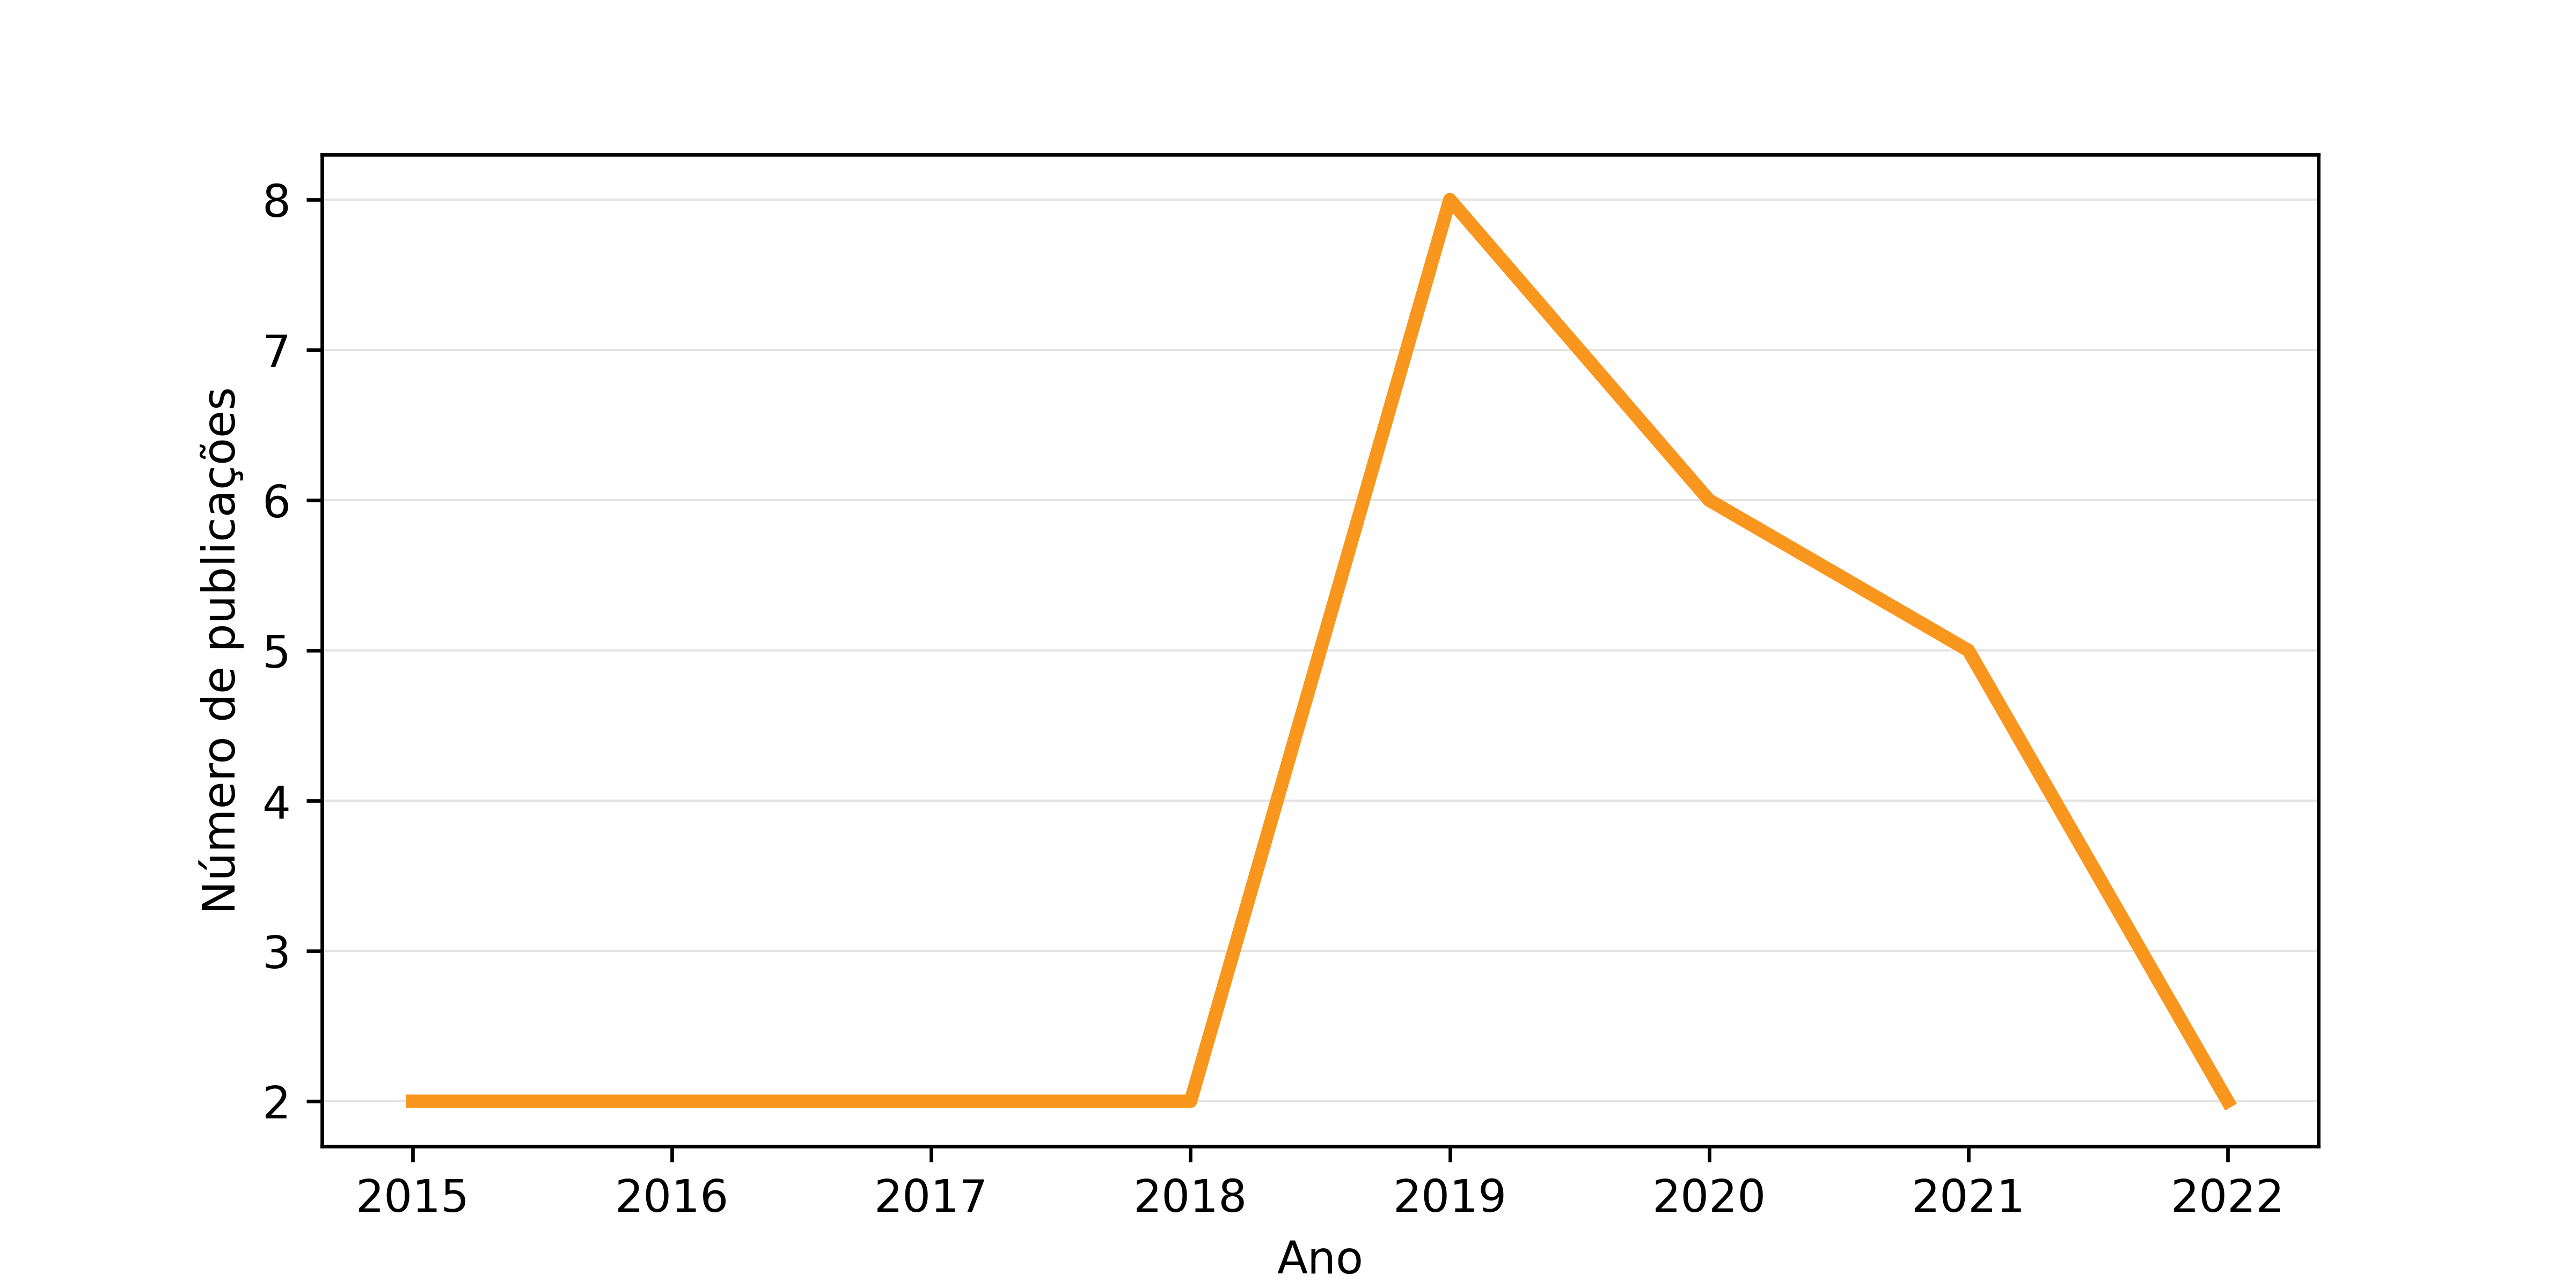
\includegraphics[width=0.7\linewidth]{USPSC-img/pubVulAmount.png}
        \end{center}
        \fonte{elaborada pelo autor.}
    \end{figure}
    
    A avaliação desses resultados conduz a uma conclusão que, embora semelhante à anterior, revela uma oscilação notória. No ano de 2019, um pico significativo na quantidade de artigos publicados denota um interesse acentuado e um maior reconhecimento por parte da comunidade científica acerca das \index{Vulnerabilidade}vulnerabilidades associadas ao \index{OPC UA}OPC UA. Entretanto, a partir de 2020, constata-se uma inversão na tendência, com uma redução na quantidade de publicações. Esse declínio pode estar relacionado a diversos fatores interconectados, conforme descrito anteriormente. Contudo, vale ressaltar a importância do tema do presente estudo, uma vez que se sabe a incerteza da natureza das ameaças e a dinâmica das vulnerabilidades em ambientes industriais utilizando esse protocolo.
    
    \section{Objetivos} \label{sec:objetivos}

    Tendo em vista a relevância do tema, o presente estudo propõe uma investigação detalhada de ataques cibernéticos em redes \index{OPC UA}OPC UA, visando desenvolver, implementar e validar uma bancada experimental para simulações de intrusões em sistemas de automação e controle industriais. Busca-se compreender as potenciais fragilidades que podem comprometer a segurança destas redes, identificando os principais pontos de risco e explorando possíveis contramedidas para mitigar as \index{Ameaça Cibernética}ameaças identificadas.

    Observa-se um caráter desafiador ao objetivo, uma vez que a complexidade e a diversidade dos dados trafegados pelas camadas do protocolo demandam um alto grau de especialização em \index{Segurança Cibernética}segurança cibernética e técnicas avançadas de engenharia de redes.

    Dentro desse contexto, os objetivos específicos a serem atingidos pela metodologia proposta são:
    
    \begin{itemize}
        \item Investigar e compreender os princípios e conceitos fundamentais das redes \index{OPC UA}OPC UA, a fim de identificar os principais desafios e \index{Ameaça Cibernética}ameaças relacionados à segurança nestas redes;
        \item Propor e desenvolver uma bancada experimental como ambiente industrial de simulação de \index{Ataque Cibernético}ataques cibernéticos;
        \item Investigar, selecionar e aplicar alguns ataques comuns para IIoT e demonstrar a reação do protocolo OPC UA às intrusões na rede;
        \item Analisar o cenário de ataque do ponto de vista do invasor, a fim de identificar os desafios da segurança, encontrar possíveis novas vulnerabilidades e propor contramedidas para mitigação.
    \end{itemize}
    
    \section{Estrutura dos Capítulos} \label{sec:estCapitulos}

    % A dissertação está organizada em capítulos que apresentam aspectos dos trabalhos desenvolvidos. No \autoref{cap:refTeorico}, uma revisão da literatura é apresentada. \autoref{cap:desenvolvimento}. \autoref{cap:resultados}. \autoref{cap:conclusao}. 

    % A dissertação está organizada em capítulos que apresentam aspectos dos trabalhos desenvolvidos. No \autoref{cap:refTeorico}, uma revisão da literatura acerca do tema é apresentada, assim como os conceitos teóricos referentes às redes OPC UA, os fundamentos da segurança cibernética e as técnicas de análise de vulnerabilidades voltadas às estas redes. Aborda-se também alguns trabalhos correlatos ao presente trabalho. O \autoref{cap:desenvolvimento} apresenta os principais materiais utilizados na bancada experimental para ensaios de intrusão, juntamente com os ataques cibernéticos escolhidos e a metodologia utilizada para analisá-los. \autoref{cap:resultados}. Por fim, o \autoref{cap:cronograma} expõe o cronograma proposto para a finalização correta deste mestrado. 

    Esta dissertação está estruturada em capítulos que abordam os diferentes aspectos dos trabalhos desenvolvidos. O \autoref{cap:refTeorico} apresenta uma revisão abrangente da literatura relacionada ao tema, incluindo os conceitos teóricos fundamentais das redes OPC UA, os princípios essenciais da segurança cibernética e as técnicas de análise de vulnerabilidades aplicadas a essas redes. Além disso, são discutidos trabalhos anteriores relevantes para o contexto deste estudo. No \autoref{cap:desenvolvimento}, os principais componentes e materiais empregados na montagem da bancada experimental para a realização dos ensaios de intrusão são detalhados. Também são descritos em pormenor os ataques cibernéticos selecionados e a metodologia adotada para sua análise. Os resultados esperados são apresentados no \autoref{cap:resultados}. Por fim, o \autoref{cap:cronograma} delineia o cronograma proposto para a conclusão bem-sucedida deste programa de mestrado.

\chapter{Referencial Teórico} \label{cap:refTeorico}

    Este capítulo serve como uma base para a compreensão dos fundamentos teóricos e estruturas conceituais que informam a pesquisa, aprofundando-se na literatura relevante e nos conceitos teóricos associados às redes \index{OPC UA}OPC UA, fundamentos da \index{Segurança Cibernética}segurança cibernética e a aplicação de técnicas de análise de vulnerabilidades para aprimorar a segurança dessas redes. Ao examinar a base de conhecimento existente, uma estrutura teórica é estabelecida, a fim de formular estratégias eficazes e garantir a implementação bem-sucedida da abordagem proposta. O capítulo é finalizado com alguns estudos correlatos e como se diferem do presente trabalho.
    
    \section{Protocolos \index{IoT}IoT e \index{IIoT}IIoT} \label{sec:protocolos}
    
    A \index{Indústria 4.0}Indústria 4.0 se materializou em diversas esferas, tratando-se como a integração de inúmeras possibilidades de tecnologias para atender as demandas do mercado, tanto em relação às transformações da forma de como os processos de manufatura e máquinas são feitos, como também em relação às grandes mudanças de modelos de negócios \cite{trotta2018}. Esta onda de inovação está impulsionando as organizações a investirem em novas tecnologias, incluindo \index{IoT}Internet das Coisas e IIoT, transformando-as em realidade diária ao revolucionar como dispositivos, sistemas e aplicativos interagem e colaboram.
    
    De acordo com \citeonline{michael2016}, o termo \index{IoT}IoT foi utilizado pela primeira vez em 1999, por Kevin Ashton, que trabalhou em um padrão para marcar objetos em aplicações de logística, utilizando RFID. Desde então, os pesquisadores referem-se à expressão como a interconexão de objetos cotidianos incorporados com sensores, atuadores e capacidades de comunicação. No entanto, devido ao crescimento exponencial dos protocolos de comunicação inteligentes e da conectividade distribuída advindos dessa tecnologia, a quarta revolução incorporou essas características positivas nos processos industriais e no desenvolvimento de produtos, que, consequentemente, começaram a ter seus dados otimizados dinamicamente. A \autoref{fig:convergenceIoT} apresenta a convergência de diferentes visões destacadas pela \index{IoT}IoT.

    \begin{figure}[htbp]
        \caption{Convergência de diferentes visões destacadas pela IoT}
        \label{fig:convergenceIoT}
        \begin{center}
            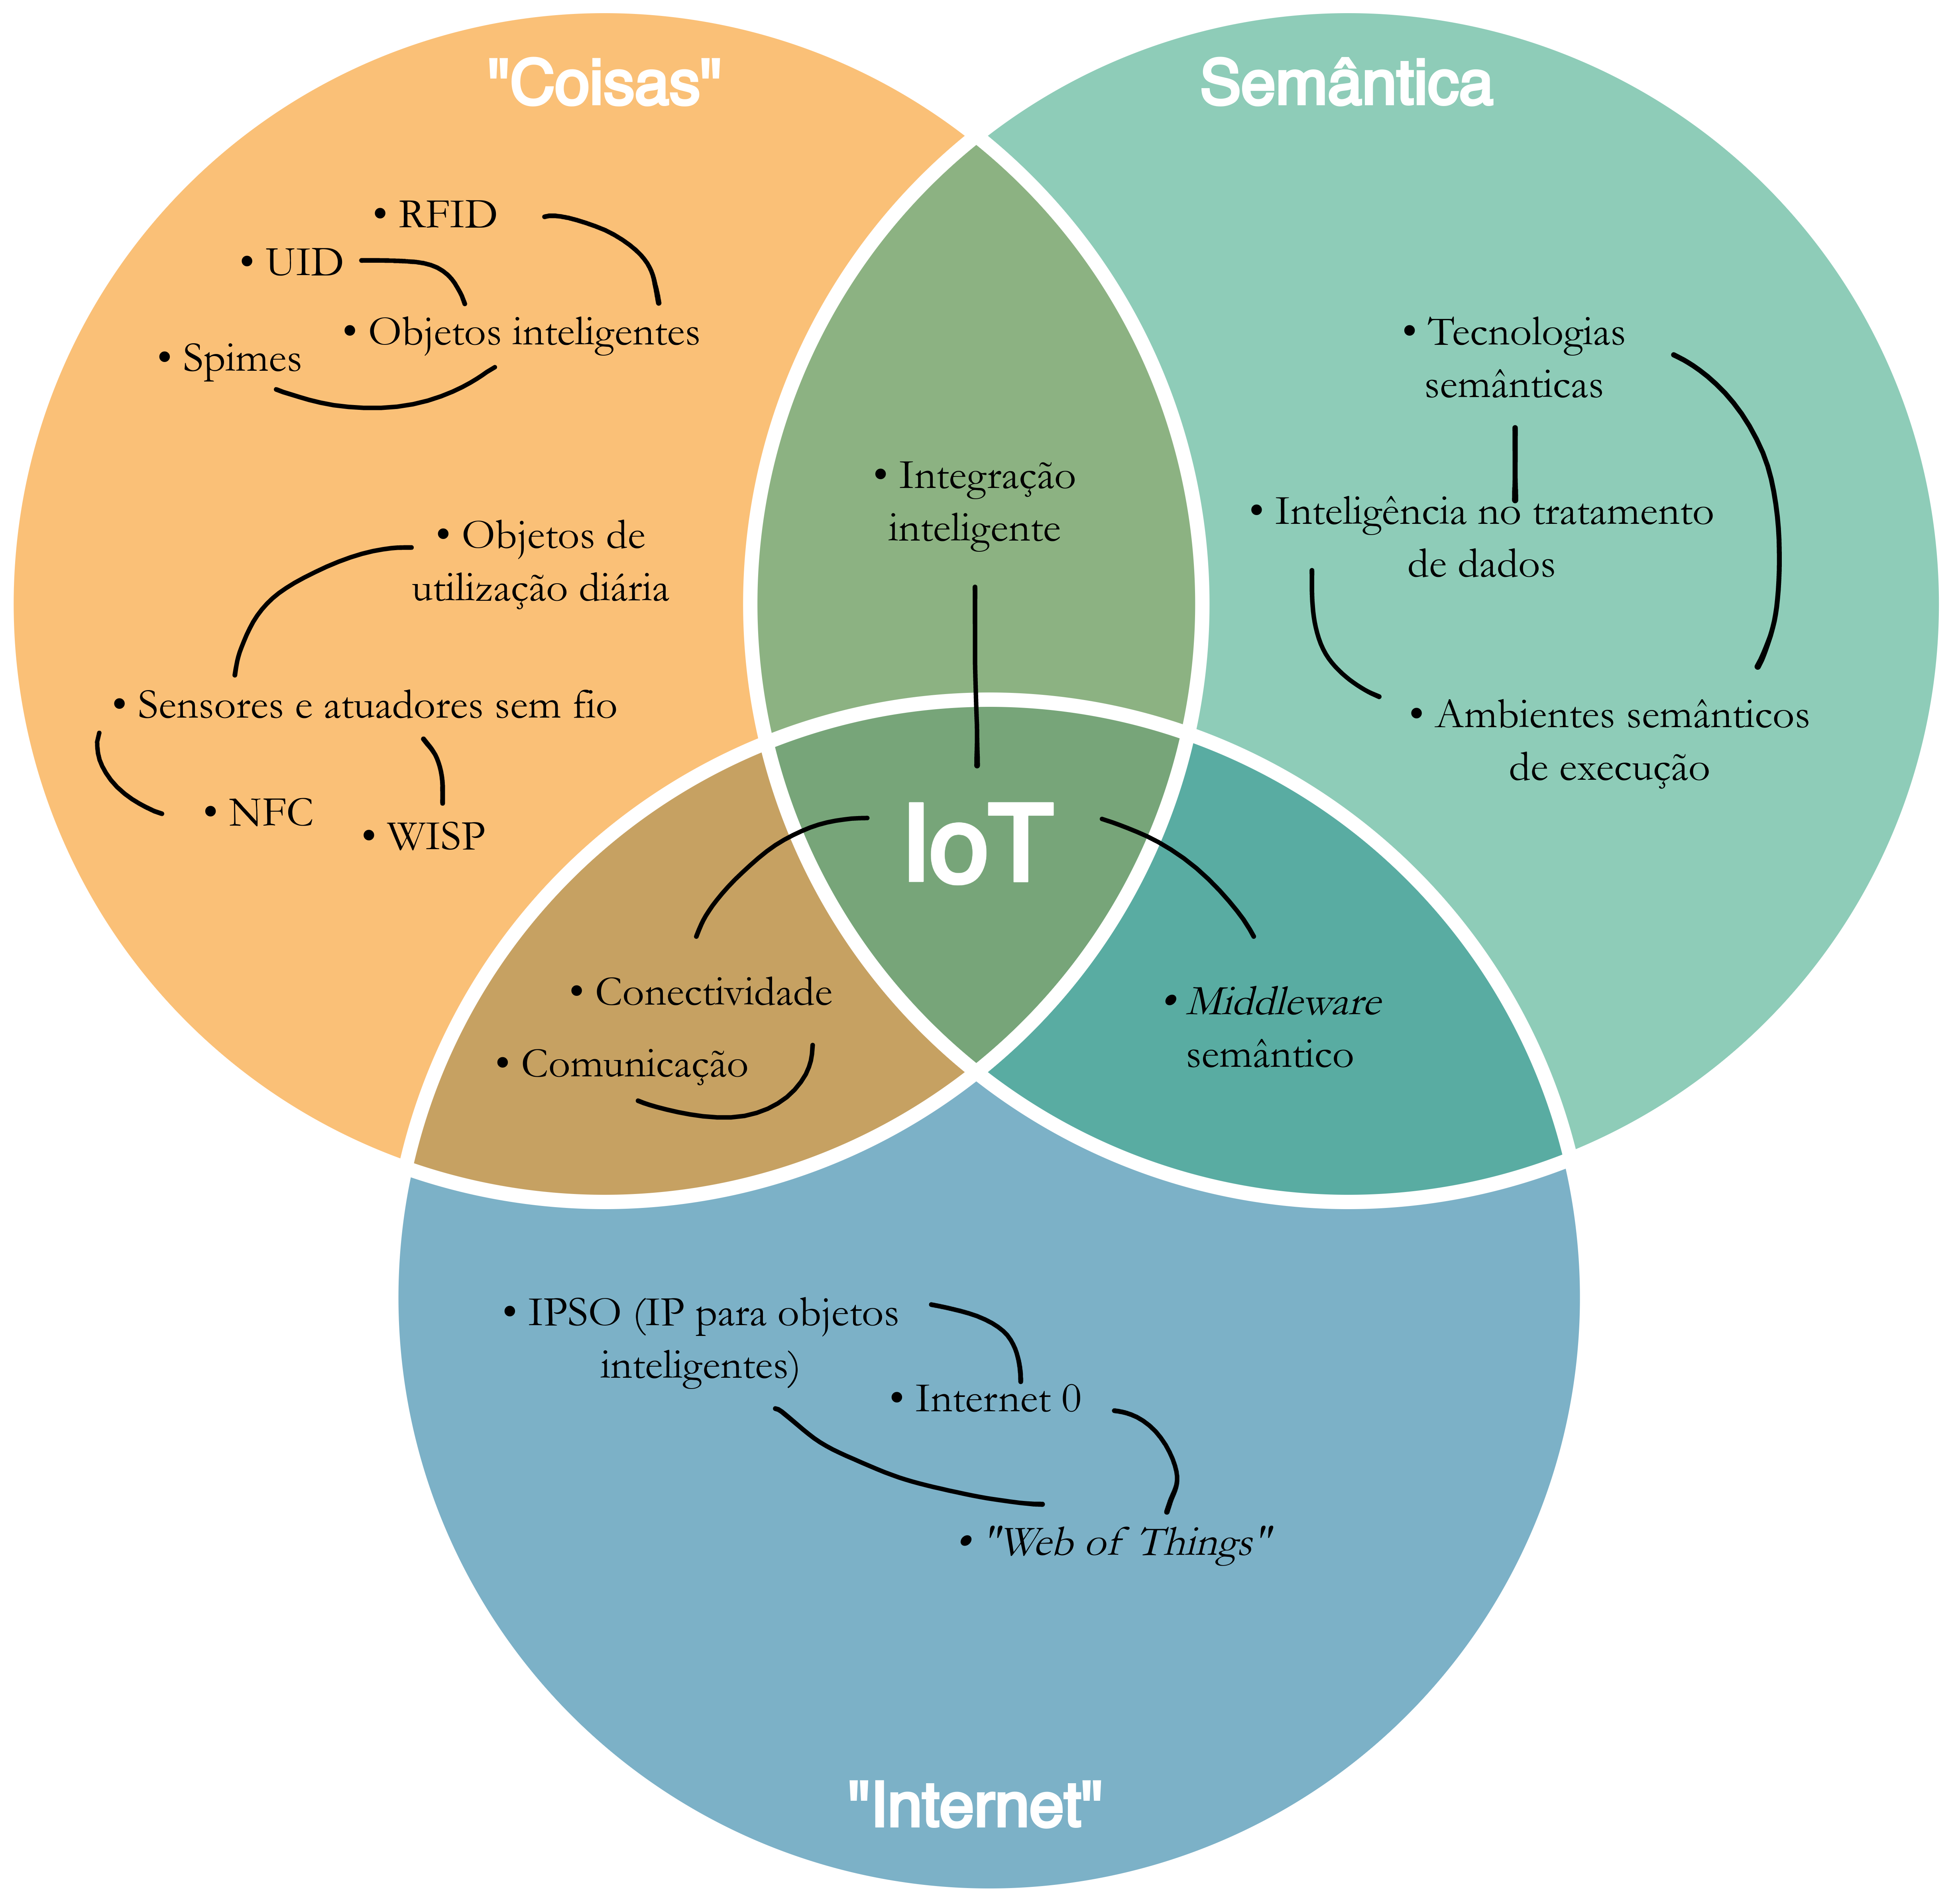
\includegraphics[width=0.7\linewidth]{USPSC-img/convergenceIoT2.png}
        \end{center}
        \fonte{adaptada de \cite{bandyopadhyay2011}}
    \end{figure}
    
    Para fortalecer o desenvolvimento no âmbito industrial, surgiu o \index{IIoT}IIoT como um novo tipo de ecossistema que envolve todos os domínios de logística, fabricação, gerenciamento e desenvolvimento. Concentra-se especificamente na aplicação da \index{IoT}IoT em ambientes industriais, viabilizando aprimoramentos em automação e eficiência e produtividade em variados setores (\textit{e.g.}, manufatura, energia, transporte e saúde). A Internet das Coisas Industrial não apenas envolve elementos de \textit{software} tradicionais, mas também requer controladores e sensores de \textit{hardware}, bem como plataformas de serviços em nuvem, para alcançar o domínio inteligente \cite{huichao2020}. A \autoref{fig:convergenceIIoT} ilustra a convergência dos tópicos de formação da \index{IIoT}IIoT.

    \begin{figure}[htbp]
        \caption{Convergência dos tópicos de formação da IIoT}
        \label{fig:convergenceIIoT}
        \begin{center}
            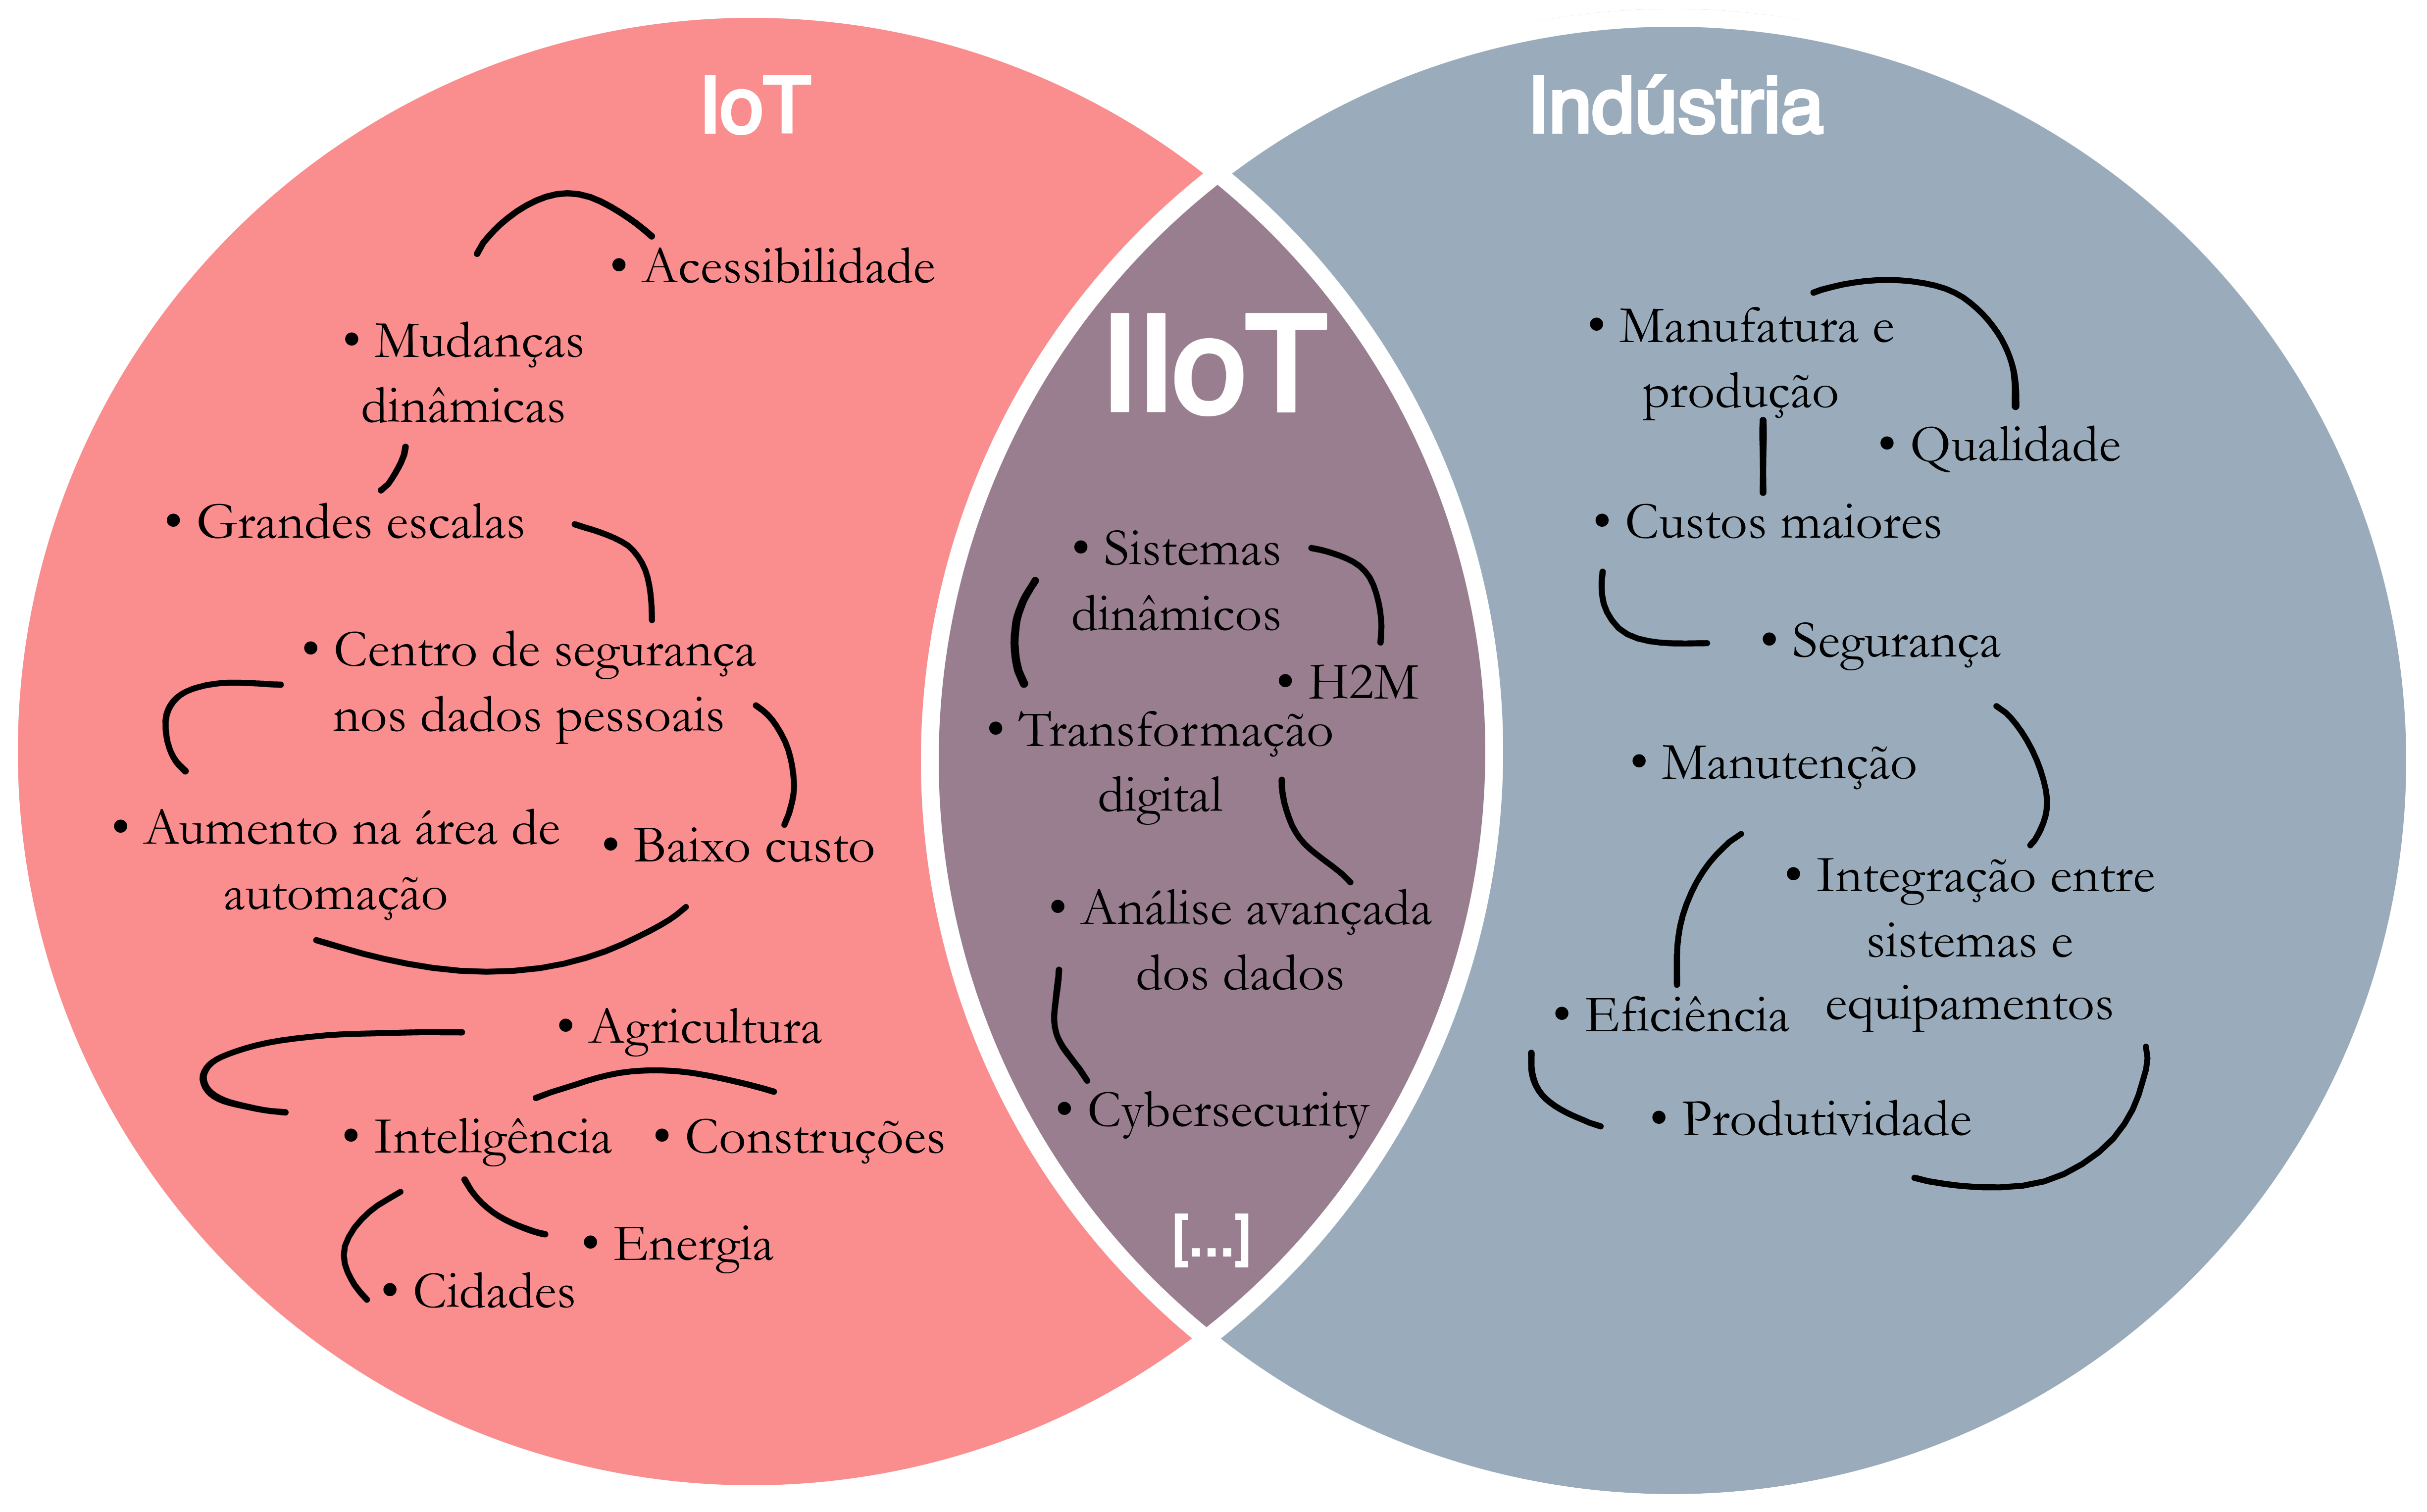
\includegraphics[width=0.7\linewidth]{USPSC-img/convergenceIIoT2.png}
        \end{center}
        \fonte{elaborada pelo autor.}
    \end{figure}
    
    Em sua escala, alcance e complexidade, a transformação digital, oriunda da atual revolução tecnológica, apresenta à sociedade desafios singulares ao alterar radicalmente nosso modo de viver e interagir. Intrinsecamente conectada à incessante troca de informações, ela atribui uma alta significância para as formas de transmissão, coleta e tratamento desses dados, que, cada vez mais abundantes, trazem informações mais completas e suficientes.

    Para que os dispositivos de transmissão de informações se comuniquem, uma linguagem formal deve ser especificada. De modo análogo à comunicação humana, estabelecer um diálogo compreensível torna-se uma tarefa árdua quando as partes envolvidas não compartilham o mesmo dialeto. Dessa forma, as linguagens especificam um conjunto de regras que asseguram uma comunicação cognoscível e a interoperabilidade entre sistemas, dispositivos e pessoas em diversos contextos.

    Tanto a \index{IoT}IoT quanto a \index{IIoT}IIoT dependem de protocolos robustos para estabelecer canais de comunicação confiáveis e seguros. Esses protocolos desempenham um papel crucial ao permitir o monitoramento, controle e gerenciamento em tempo real das implantações. Compreender os conceitos fundamentais e as características desses, é essencial para implementar e aproveitar efetivamente o potencial das tecnologias da (I)IoT.

    O termo protocolo, de acordo com \cite{persson2015}, caracteriza o conjunto de regras e orientações que redigem a comunicação e interação entre diferentes entidades ou sistemas, estabelecendo o formato, a ordem e o significado das mensagens trocadas. Projetado principalmente para garantir a interoperabilidade entre sistemas de vários fornecedores, um protocolo também simplifica a integração e o comissionamento de redes de comunicação de dados, reduzem os custos de instalação e permitem testes e validações independentes, o que, por sua vez, leva a projetos mais eficientes \cite{mohagheghi2009}.

    Os protocolos de comunicação existentes, tanto os originalmente projetados para ambientes industriais quanto os para a \index{IoT}IoT, não oferecem as características necessárias para a quantidade cada vez maior de dispositivos conectados \cite{markel2017}. Por essa razão, um novo conjunto de protocolos escaláveis e leves surgiu, dos quais se destacam o \index{OPC UA}OPC UA, MQTT, CoAP, entre outros. No entanto, neste trabalho, o protocolo \index{OPC UA}OPC UA é o único abordado, uma vez que representa o foco central desta investigação.
    
    \subsection{Principais Aspectos do Protocolo OPC UA} \label{subsec:opcUA}

        \textit{Open Platform Communications} (OPC, anteriormente conhecido como \textit{OLE for Process Control}), desenvolvido pela OPC Foundation, é um padrão de comunicação amplamente utilizado por vários anos nos mais diversificados setores da tecnologia da informação e automação industrial. De acordo com \citeonline{lange2010}, o OPC tem sido muito aceito nas últimas décadas como o padrão industrial mais popular entre usuários e desenvolvedores. A maioria dos fornecedores de IHM (Interface Homem-Máquina), SCADA (do inglês \textit{Supervisory Control and Data Acquisition}), e DCS (do inglês \textit{Distributed Control System}) da área, oferecem a tecnologia OPC como parte integrada de seus produtos.
        
        Duas etapas principais compõem o desenvolvimento desta tecnologia: (I) OPC Classic, e (II) \index{OPC UA}OPC UA. Em suma, o Classic fornece padrões de interface de comunicação neutros (no âmbito de fornecedores) para controle de processo e sistemas de automação de manufatura, incluindo acesso a dados (OPC DA), alarmes e eventos (OPC A\&E) e acesso a dados históricos (OPC HDA). Ele resolve a integração perfeita de dispositivos de campo, dispositivos de controle e sistemas de \textit{software} de automação (\textit{e.g.}, SCADA), melhorando a abertura e a interoperabilidade do sistema \cite{han2022}. No entanto, o produto desenvolvido na primeira etapa é limitado em sua capacidade de realizar aplicações integradas e em plataformas distintas e, principalmente, carece de tecnologias que o transformam em um protocolo de comunicação seguro. É por esse, e outros motivos, que a versão \textit{Unified Architecture} do OPC foi criada. Segundo \citeonline{lange2010}:
    
        \begin{citacao}
            O \index{OPC UA}OPC UA não foi planejado apenas como uma nova versão da interface padrão OPC, mas sim como uma nova visão de interoperabilidade "global" e troca de dados padronizada entre aplicações de \textit{software} independentes de fornecedores, linguagens de programação, sistemas operacionais e localização [...], ao implementar independência de plataforma, escalabilidade, alta disponibilidade, capacidade de Internet, entre outras características nesse novo protocolo.
        \end{citacao}
    
        Aproveitando as tecnologias de Serviços Web, XML e .NET, o UA é caracterizado por sua definição de objeto unificado e apresenta uma arquitetura completamente orientada a serviços (SOA, do inglês \textit{Service Oriented Architecture}). Também pode ser integrado com as mais recentes tecnologias, como: \textit{Time Sensitive Networking} (TSN) e 5G \cite{han2022}, e os dados de comunicação podem ser codificados usando diferentes métodos. Dentre as principais vantagens do protocolo, se destacam:
    
        \begin{itemize}
            \item \underline{Independência de plataforma}: por oferecer diferentes pilhas de \textit{software} em C/C++, .Net e Java, é possível desenvolvê-lo em vários sistemas e dispositivos embarcados, não limitando apenas à plataforma da Microsoft, como no OPC Classic;
            \item \underline{Mecanismos de segurança aprimorados}: inclui um conjunto completo de mecanismos de comunicação segura, na qual requer autenticação de duplo sentido para ambos os certificados e estabelecimento de canais seguros;
            \item \underline{Modo de acesso unificado aos dados}: ao integrar os dados atuais, notificações de eventos e histórico no mesmo espaço de endereço na modelagem de informações, o \index{OPC UA}OPC UA unifica as diferentes funções anteriores, por meio de apenas uma chamada;
            \item \underline{Suporte a estruturas de dados complexas}: as especificações existentes oferecem apenas uma organização hierárquica simples de itens, enquanto o \index{OPC UA}OPC UA oferece metamodelos de informações que podem ser facilmente estendidos, sendo possível incluir e excluir as ligações entre esses modelos de dados.
        \end{itemize}
        
        Todas as especificações lançadas pela OPC Foundation para o protocolo \index{OPC UA}OPC UA estão disponibilizadas em 24 partes, pela última versão de lançamento 1.05.02 do documento `OPC UA Specification' \cite{opc2022}. As partes 1 a 7 do documento apresentam as principais características da tecnologia, assim como o modo de segurança, espaço de endereçamento, conjunto de serviços, modelo de informação padrão, mapeamentos e perfis de serviço. As partes 8 a 13 estão relacionadas às definições de tipo de acesso a dados gerais padrão, como acesso a dados, alarmes e condições, programas, acesso histórico, descoberta e agregados. Alguns dos principais conceitos teóricos do protocolo concernentes para esta dissertação estão apresentados nas subseções abaixo, como o \textit{Address Space}, o \textit{Information Model}, a transmissão dos dados, a segurança implementada em cada camada e o processo de conexão entre um cliente e servidor OPC UA.
    
        \subsubsection{Espaço de Endereçamento e Modelo de Informação}

        Conceitua-se de forma concisa o Espaço de Endereço e Modelo de Informação (do inglês \textit{Address Space} e \textit{Information Model}) como, respectivamente, a fundação e componente central do \index{OPC UA}OPC UA. Pode-se equiparar esses dois conceitos, analogamente, à estrutura óssea e ao coração no corpo humano, na devida ordem supracitada. O \textit{Address Space} representa uma ampla variedade de informação, incluindo instâncias de objetos, variáveis e tipos \cite{gong2020}. O \index{OPC UA}OPC UA propõe um \textit{Address Space} consistente e um modelo de serviço, e isso ajudará a unificar dados, eventos e informações históricas no espaço de endereço do mesmo servidor \cite{ren2019}.
        
        Os \textit{Nodes} se caracterizam como os componentes em um Espaço de Endereço, sendo que cada um recebe uma classe correspondente a um elemento específico do modelo de objeto (do inglês \textit{Object Model}), incluindo variáveis, métodos e eventos. Essas classes servem coletivamente como os `metadados' do \textit{Address Space} e cada \textit{Node}, uma instância de uma classe. 
        
        A definição de classe contempla atributos e referências. Os Atributos (do inglês \textit{Attributes}) formam os componentes fundamentais de uma classe e cada definição de atributo inclui um ID, nome, descrição, tipo de dados e indicadores de obrigatoriedade. As referências (do inglês \textit{References}), por sua vez, indicam o relacionamento entre dois \textit{Nodes} conhecidos, e uma referência é determinada exclusivamente pelo nó de origem, o de destino, a semântica da referência e a sua direção.

        A \autoref{fig:opcuaArqCS} apresenta a arquitetura cliente-servidor do \index{OPC UA}OPC UA, ilustrando as conexões entre os conceitos supracitados.

        \begin{figure}[htbp]
            \caption{Arquitetura Cliente-Servidor do OPC UA}
            \label{fig:opcuaArqCS}
            \begin{center}
                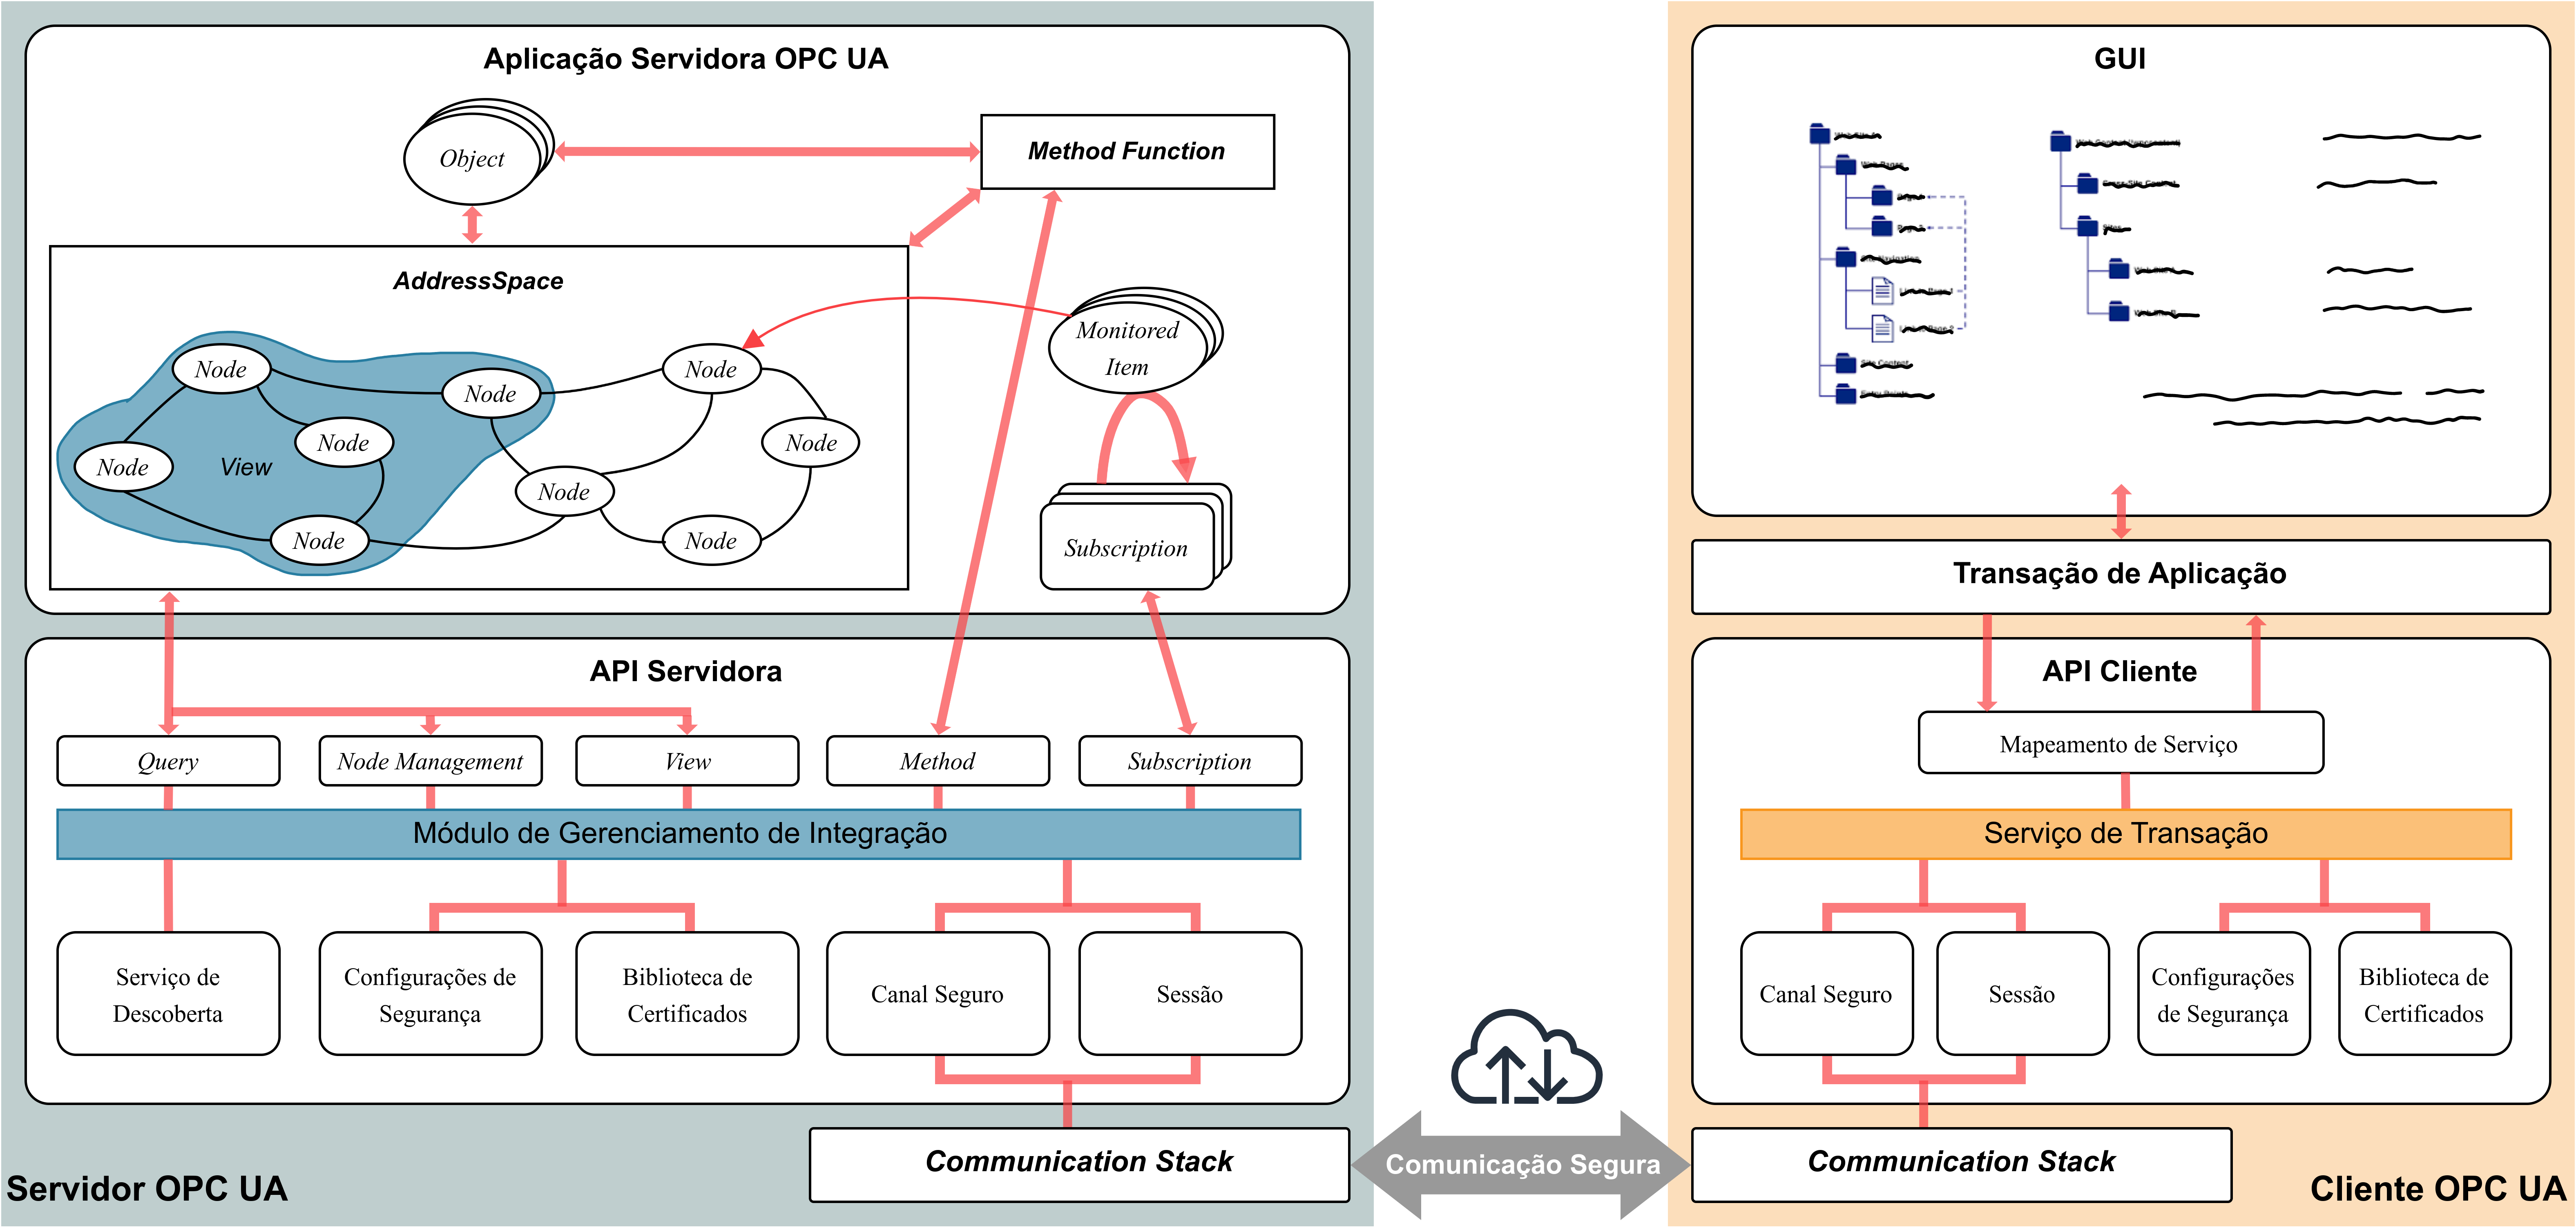
\includegraphics[width=1\linewidth]{USPSC-img/opcuaClientServerArc1.png}
            \end{center}
            \fonte{adaptada de \cite[Parte 6]{opc2022} e \cite{huang2010}.}
        \end{figure}

        O \textit{Information Model} é composto principalmente de \textit{Nodes} e \textit{References}, possibilitando a representação de diversas informações estruturadas e hierárquicas. Com funcionalidade abrangente orientada a objetos, até estruturas complexas de várias camadas podem ser modeladas e estendidas. O \index{OPC UA}OPC UA oferece uma estrutura de modelo fundamental e a possibilidade de criação de outros complementares para aplicações específicas, a fim de aprimorar ainda mais o sistema.

        A relação entre modelos de informação fundamental e específicos do usuário são representados na \autoref{fig:opcuaArq}. A aplicação \index{OPC UA}OPC UA apresenta a flexibilidade em seu desenvolvimento por poder ser iniciada a partir de um Modelo de Informação principal ou complementar padronizado que se alinha conforme o domínio específico. Com isso, aproveitando a abordagem de modelagem orientada a objetos do protocolo e utilizando o conjunto predefinido de serviços de acesso e manipulação, a interoperabilidade excepcional pode ser alcançada pelo sistema \cite{gong2020}.

        \begin{figure}[htbp]
            \caption{Infraestrutura de modelos do OPC UA}
            \label{fig:opcuaArq}
            \begin{center}
                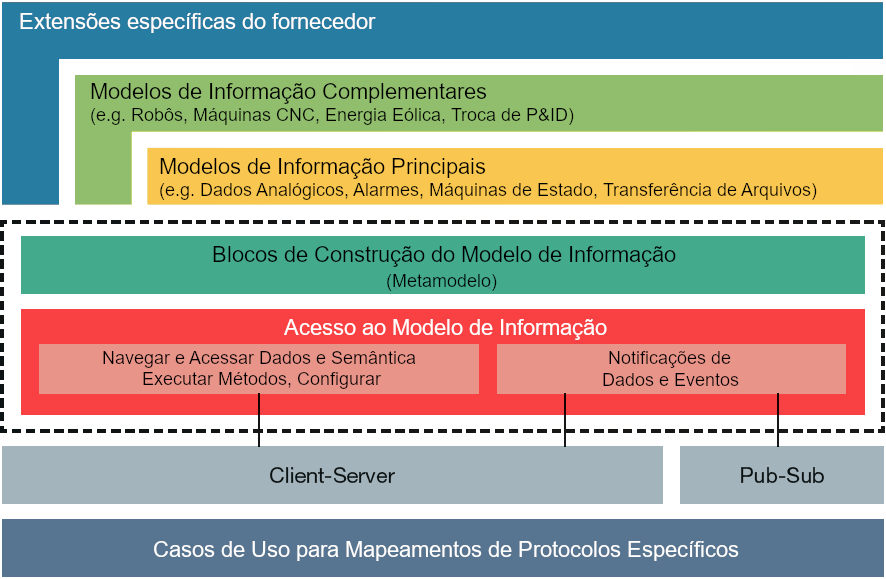
\includegraphics[width=0.9\linewidth]{USPSC-img/opcuaArq.png}
            \end{center}
            \fonte{adaptada de \cite{opc2019}.}
        \end{figure}

        \subsubsection{Métodos de Comunicação}

        O \index{OPC UA}OPC UA abrange mapeamentos de elementos independentes de protocolo para protocolos de transporte e segurança padronizados. Atualmente, a transmissão de dados pode ser realizada por meio de três métodos distintos: TCP/IP, SOAP/HTTP e HTTPS. Em termos de implementação de segurança, obrigatória para todas as variantes, o \index{OPC UA}OPC UA define \textit{UA Secure Conversation} e \textit{WS Secure Conversation} para TCP/IP e SOAP/HTTP, como os respectivos protocolos  \cite{neumann2015}.
        
        Em relação à codificação de mensagens e apresentações de dados, o \index{OPC UA}OPC UA oferece duas opções principais: UA-XML e UA-\textit{Binary}, nos quais utilizam, respectivamente, esquemas de codificação para Serviços Web e formatos binários, descritos na Parte 6 do documento de especificações \cite{opc2022}, para comunicação eficiente em sistemas de alta velocidade ou embarcados. Com isso, permitem flexibilidade na escolha do formato apropriado para transmissão e representação de dados eficientes. A \autoref{fig:ua-osi} ilustra essas abordagens do UA categorizadas no modelo de referência OSI (do inglês \textit{Open Systems Interconnection}), destacando os componentes de comunicação supracitados. %, sustentando a interoperabilidade e segurando do \index{OPC UA}OPC UA ao realizar um `desvio' por algumas camadas do modelo.
        
        \begin{figure}[htbp]
            \caption{Categorização da comunicação OPC UA no modelo de referência OSI}
            \label{fig:ua-osi}
            \begin{center}
                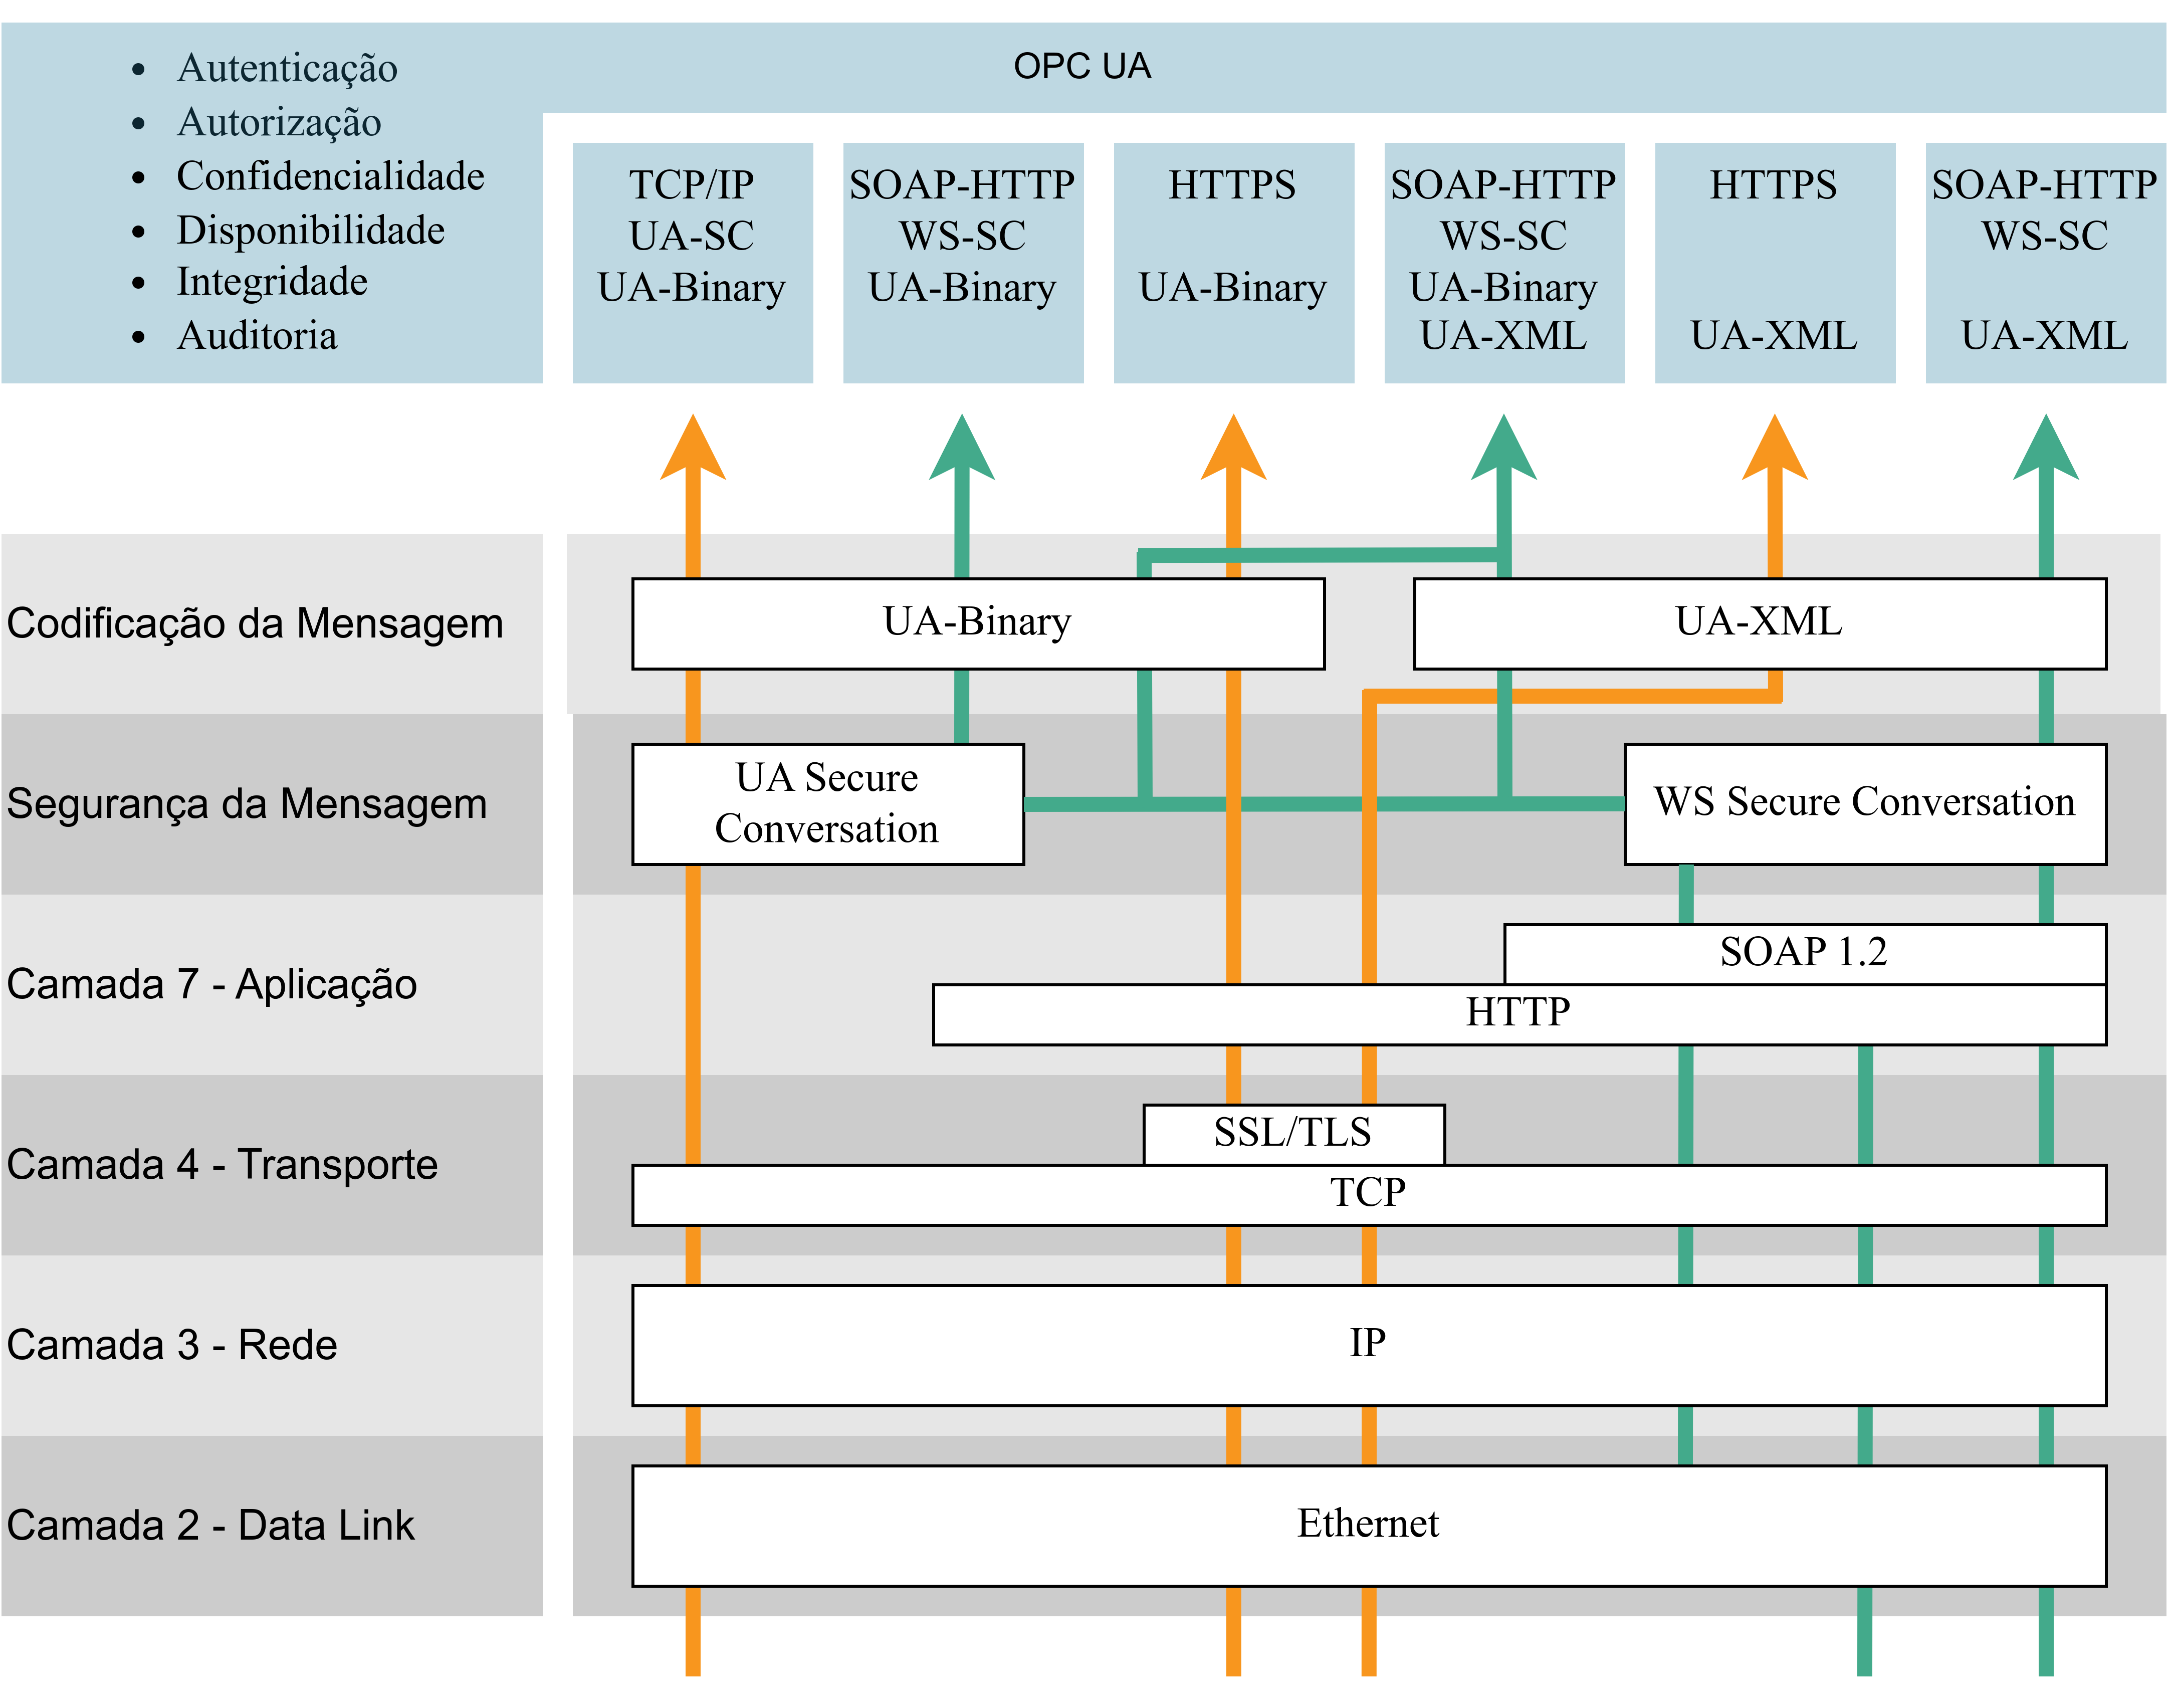
\includegraphics[width=0.9\linewidth]{USPSC-img/ua-osi.png}
            \end{center}
            \fonte{adaptada de \cite{neumann2015}.}
        \end{figure}

        \subsubsection{Escopo de Proteção}

        A segurança por muito tempo foi negligenciada, resultando no reconhecimento tardio de sua gravidade e na adoção vagarosa de medidas protetivas. Esse cenário foi especialmente evidenciado em ambientes industriais, cujas preocupações com segurança foram historicamente abordadas em conjunto com a \index{Tecnologia da Informação}TI. No entanto, à medida que a interconexão digital avança, a necessidade de proteção contra uma crescente gama de ataques cibernéticos em sistemas ciber-físicos tornou-se inegável, não apenas na camada de aplicação, mas em toda a infraestrutura desses ambientes críticos.
        
        O \index{OPC UA}OPC UA foi desenvolvido com foco na resolução desse problema histórico, ao tratar de questões desse tipo em diversas camadas. Seu escopo de proteção é dividido na segurança da informação pela tríade CIA (do inglês \textit{Confidentiality, Integrity and Availability}) e pelo \textit{Framework} AAA - autenticação, autorização e auditoria.
        
        Na camada de aplicação, a autenticação e a autorização do usuário são cruciais. Autenticar o acesso envolve a verificação da identidade do cliente usando métodos como: senhas, certificados X.509V3 ou \textit{tokens} de segurança, conforme supracitado. Por outro lado, autorizar esse acesso implica na sua concessão ou negação a serviços específicos. A documentação de especificação do protocolo não alude como os usuários devem autenticar ou autorizar seus direitos, no entanto, fornece os meios para tal implementação. As aplicações \index{OPC UA}OPC UA, tanto cliente quanto servidora, também devem se identificar durante o estabelecimento da comunicação segura usando certificados, permitindo aceite ou não da requisição.
        
        A camada de comunicação fornece um canal seguro através do qual os dados são transmitidos do cliente para o servidor. Essa mensagem secreta é utilizada para derivar as \textit{Symmetric Keys} do processo de criptografia dos dados requeridos e respondidos, garantindo a confidencialidade da comunicação ao impedir acessos não autorizados. Da mesma forma, a integridade é mantida por meio de assinaturas para verificar se as informações recebidas pelo cliente correspondem ao que foi enviado pelo servidor. A \autoref{subsubsec:conn} detalha o procedimento envolvido no estabelecimento do canal seguro entre servidor e cliente OPC UA.

        Por fim, as aplicações geram registros de auditoria que abrangem vários eventos, como tentativas de conexão, negociações de opções de segurança, alterações de configuração e sistema, interações do usuário e rejeições de sessão. O suporte a essas trilhas de auditoria de segurança é oferecido por meio de dois mecanismos: (I) a garantia da rastreabilidade entre os \textit{logs}, por meio de um identificador local na solicitação; e (II) a definição de parâmetros para inclusão nos registros de auditoria (parâmetros descritos pela Parte 5 das especificações).

        Mesmo com toda sua construção voltada para fortificar o sistema contra-ataques, o \index{OPC UA}OPC UA encontra desafios de segurança internos e externos, visto que a diversidade de protocolos na transmissão das mensagens herda os riscos de segurança dos mesmos. Assim, o estabelecimento de tecnologias robustas de segurança de rede é imperativo para lidar efetivamente com esses desafios.

        \subsubsection{Processo de Conexão Segura} \label{subsubsec:conn}

        O canal seguro estabelecido em uma comunicação OPC UA deve respeitar uma série de medidas no estabelecimento e no término da conexão, como a negociação de segurança, a decisão do algoritmo criptográfico e as políticas e perfis de segurança utilizados. A \autoref{fig:seqConn} apresenta o diagrama de sequências desse processo.

        \begin{figure}[htbp]
            \caption{Processo de criação e encerramento de conexão no OPC UA}
            \label{fig:seqConn}
            \begin{center}
                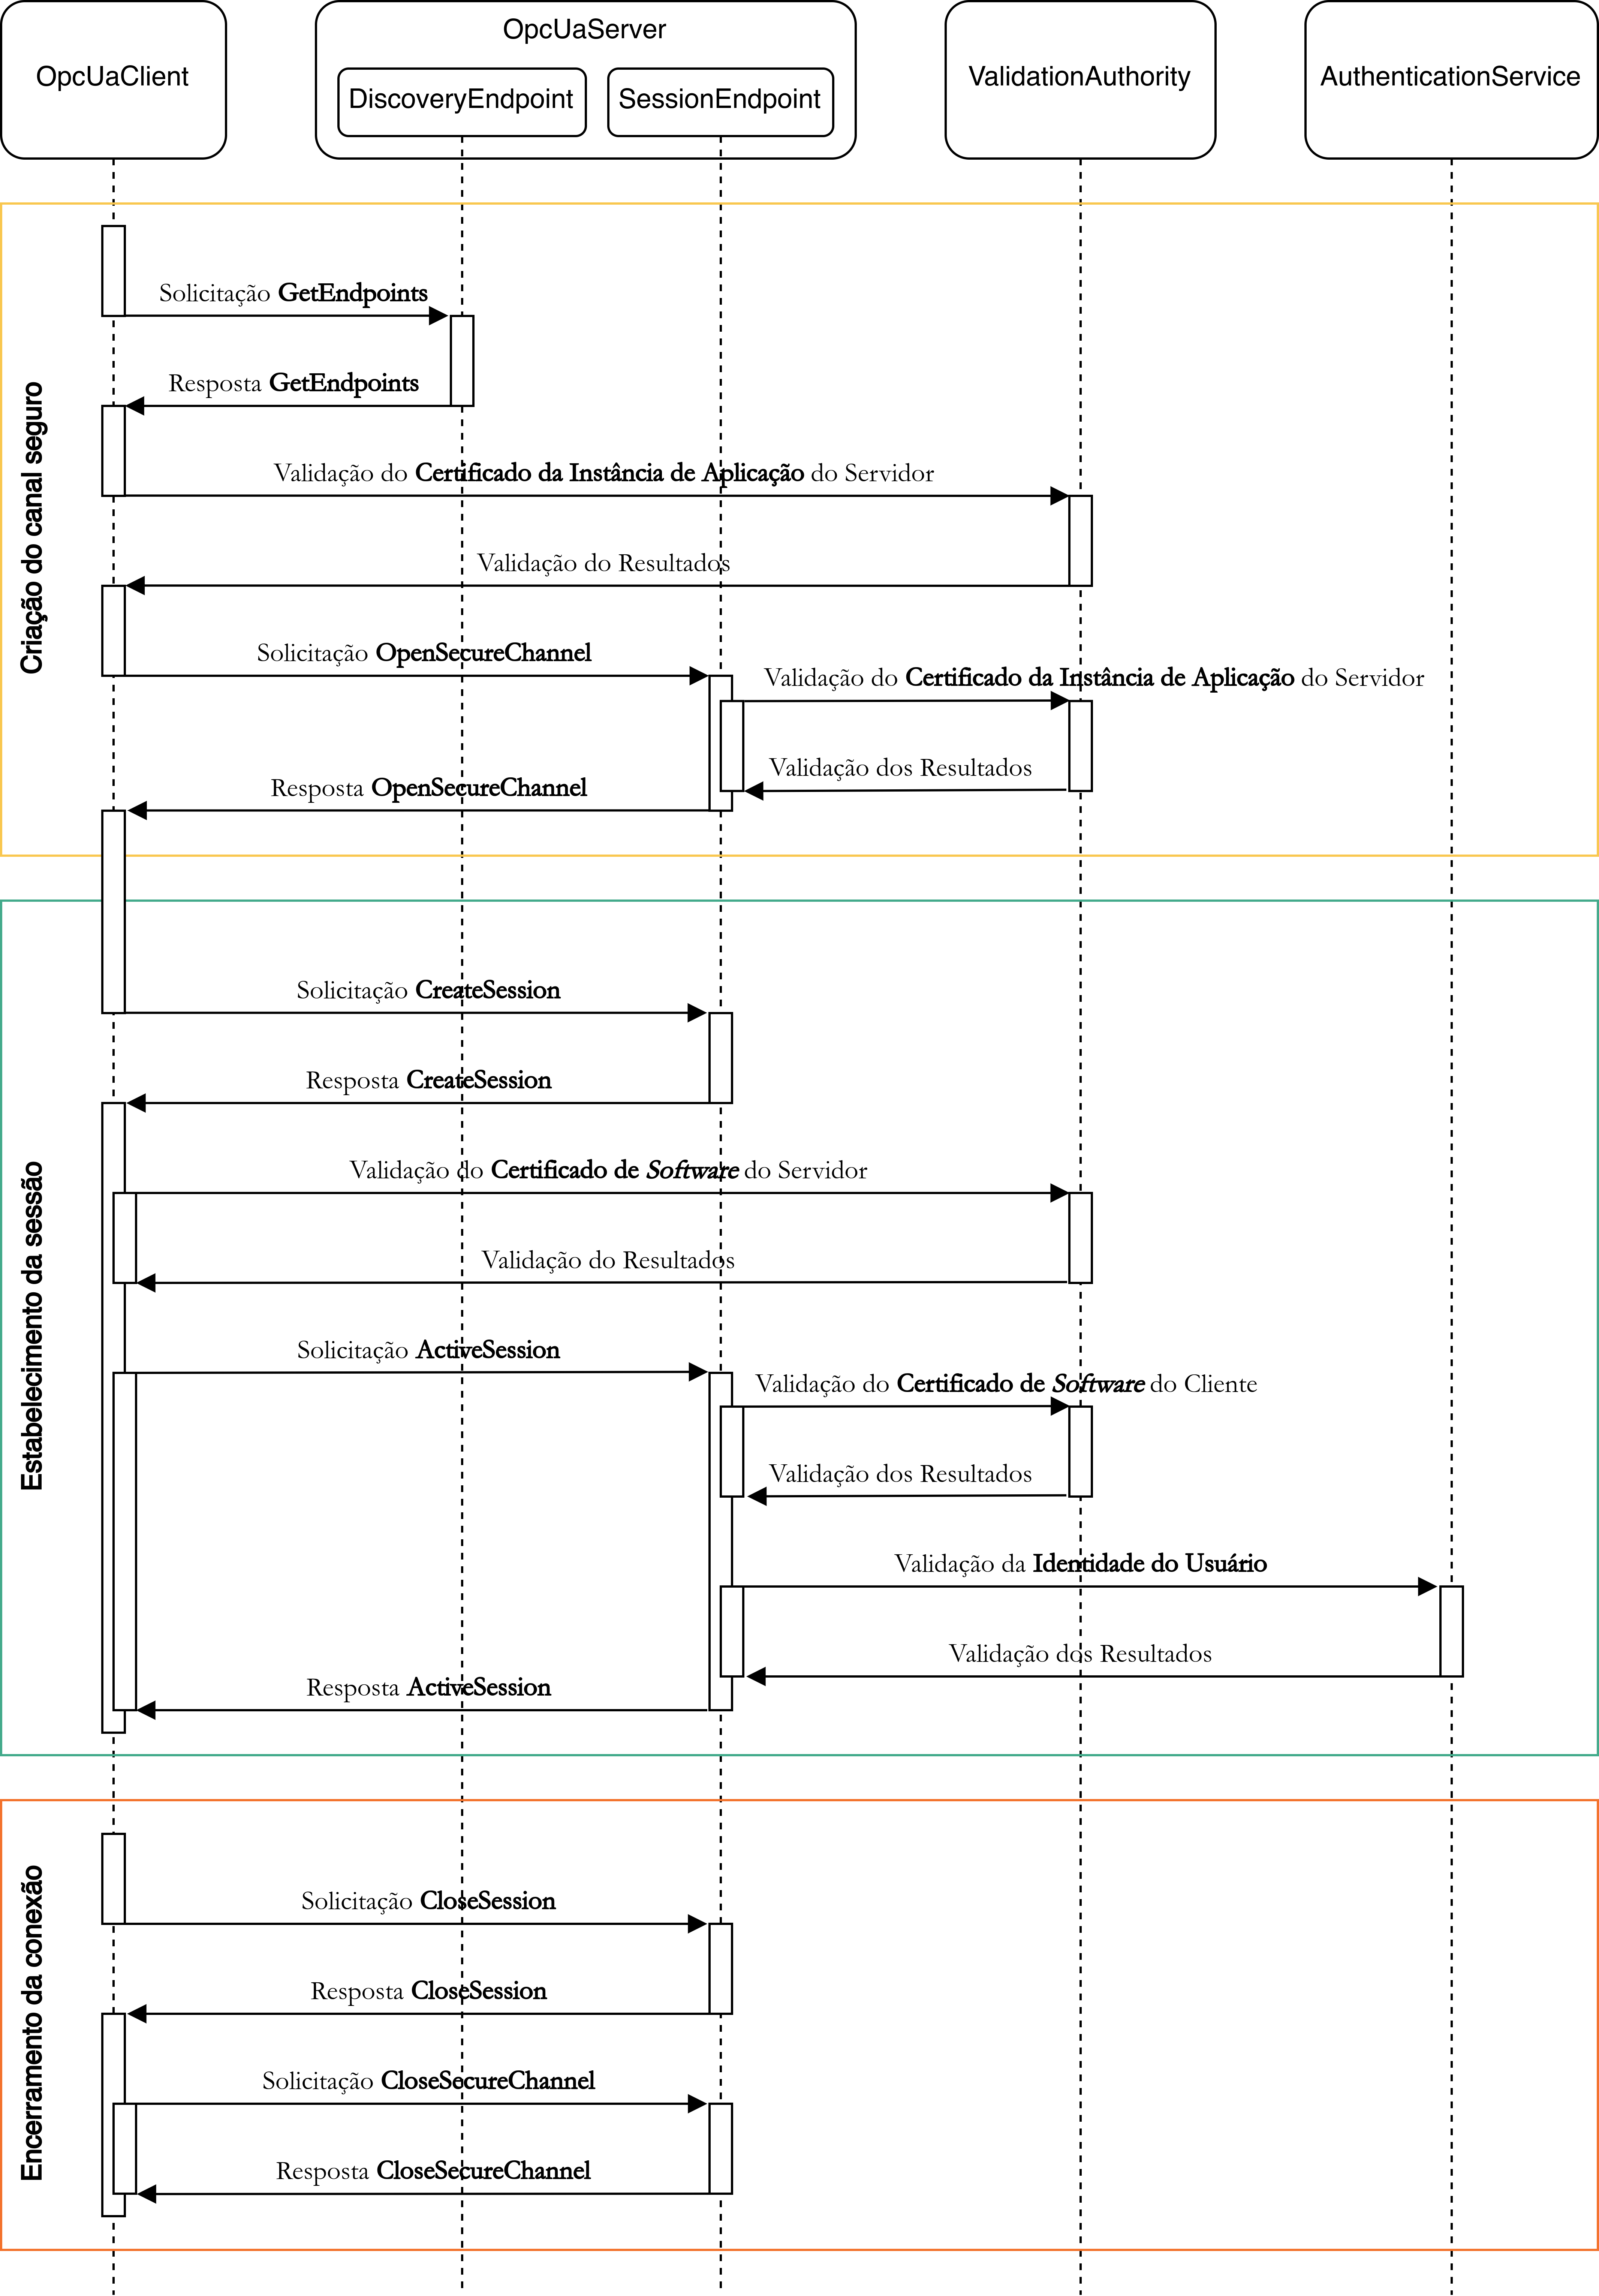
\includegraphics[width=0.972\linewidth]{USPSC-img/seqConn.png}
            \end{center}
            \fonte{adaptada de \cite{mahnke2009}.}
        \end{figure}

        Na etapa da criação da conexão, as diferentes opções de configuração do servidor são coletadas pelo cliente, caso esse não esteja pré-configurado. Uma solicitação \textbf{GetEndpoints} não segura é enviada do cliente ao \textbf{DiscoveryEndpoint} do servidor, a fim de obter as descrições dos \textbf{Endpoints} de sessão existentes, incluindo a configuração de segurança. Uma vez que essas informações são coletadas, o cliente seleciona o \textbf{Endpoint} e valida o certificado da instância de aplicação do servidor. 
        
        A segunda etapa ocorre caso o certificado seja considerado confiável após a validação. Uma solicitação \textbf{OpenSecureChannel} é criada e enviada ao \textbf{Endpoint} de sessão do servidor, incluindo a Política de Segurança e Modo de Segurança. O OPC UA incorpora um modelo de segurança flexível que consiste em três modos, descritos pelo \autoref{qdr:secureModes}.

        \begin{quadro}[htbp]
            \caption{\label{qdr:secureModes}Modos de segurança do OPC UA}
            \begin{tabular}{|M{3.60cm}|p{11.50cm}|}
                \hline
                \thead{Modos} & \thead{Descrição} \\
                \hline
                \textit{None}  & $\sbullet$ Nenhuma segurança \\
                \hline
                \multirow{4}{*}{\textit{Sign}} & $\sbullet$ Codificado com a chave privada do remetente \\
                    & $\sbullet$ Somente o proprietário do certificado possui a chave privada \\
                    & $\sbullet$ Qualquer pessoa pode verificar a identidade \\
                    & $\sbullet$ Fornece autenticidade \\
                \hline
                \multirow{5}{*}{\textit{Sign\&Encrypt}} & $\sbullet$ Adiciona criptografia para assinar \\
                    & $\sbullet$ Codificação com chave pública do receptor \\
                    & $\sbullet$ Qualquer pessoa pode criptografar \\
                    & $\sbullet$ Somente o proprietário do certificado pode ler \\
                    & $\sbullet$ Autenticidade, confidencialidade e integridade \\
                \hline
    	\end{tabular}
    	\begin{flushleft}
    		\fonte{adaptado de \cite{neu2019}.}
    	\end{flushleft}
        \end{quadro}

        Para lidar com a ameaça central da permissão de clientes maliciosos à rede, é possível alcançar a disponibilidade e a integridade do conteúdo das mensagens no modo seguro \textbf{Sign}, uma vez que as identidades dos servidores e clientes podem ser verificadas através da infraestrutura de chave pública e certificados. Para criptografar o conteúdo da comunicação de rede, utiliza-se o modo \textbf{Sign\&Encrypt}, garantindo também a confiabilidade desses dados.

        Assim sendo, uma sessão é instaurada com base no canal seguro criado pela conexão, mediante uma solicitação de \textbf{CreateSession} devidamente protegida pelo cliente. Na resposta dos servidores, por sua vez, são fornecidos os certificados de \textit{software}. A fase final do estabelecimento da comunicação é iniciada, então, após a validação bem-sucedida desses certificados por parte do cliente. Essa fase envolve a ativação da sessão criada através da solicitação \textbf{ActiveSession} ao servidor, cujas informações adicionais de credenciais do usuário e do \textit{software} estão contidas. A validação dos dados complementares representa o encerramento dessa composição de conexão, permitindo que o cliente acesse e comunique-se com o servidor exitosamente.

        O encerramento de uma conexão OPC UA ocorre por meio das solicitações \textbf{CloseSession} e \textbf{CloseSecureChannel}. A especificação do OPC UA \cite{opc2022} afirma que as mensagens de encerramento sejam apenas assinadas, pois nenhuma informação secreta é transmitida nessa etapa.

        % Os perfis (profiles) englobam a funcionalidade que uma aplicação suporta para estar em conformidade. Além disso, alguns perfis incluem funções de segurança, como o algoritmo de criptografia implementado. A escolha do mecanismo de segurança a ser usado é decidida mutualmente pelo cliente e pelo servidor. Ele é identificado por um URI e contém o nome exclusivo do algoritmo de segurança utilizado. Por exemplo, http:// opcfoundation.org/UA/SecurityPolicy#Basic128Rsa15, este URI define que o algoritmo AES com 128 bits é usado para criptografar e assinar mensagens de forma simétrica, e no caso de operação assimétrica, é usado o algoritmo RSA1.5. 2.2.1 Políticas de segurança OPC UA suportadas para Cliente-Servidor: • Aes128-Sha256-RsaOaep: Esta faceta de segurança define uma política de segurança que é usada quando há uma necessidade média de segurança. A infraestrutura de PKI é obrigatória para isso. À medida que o poder computacional aumenta, espera-se que as políticas de segurança expirem. O Instituto Nacional de Padrões e Tecnologia (NIST) ajuda a fornecer diretrizes sobre a data esperada de expiração da política de segurança. As diretrizes especificam a data em que a política deve ser atualizada ou se deve ser substituída por um algoritmo mais seguro. Embora as diretrizes não mencionem se o algoritmo falhou. Esta política de segurança em particular não tem data de término até o momento [15]. • Aes256-Sha256-RsaPss: Esta política de segurança é usada quando há uma alta necessidade de segurança. A infraestrutura de PKI é obrigatória para isso. O NIST fornece as mesmas diretrizes para esta política de segurança, mencionando a data de expiração junto com a necessidade de atualização ou substituição da política por uma mais segura [15]. • Basic128Rsa15 (obsoleta): Esta política de segurança é usada quando se necessita de segurança média. A infraestrutura de PKI é necessária também. O NIST fornece as mesmas diretrizes para esta política de segurança. O NIST recomendou aos usuários desta política que atualizassem as chaves com menos de 2048 bits em 2010. Além disso, eles também recomendaram em 2012 que as políticas usando chaves com menos de 2048 bits fossem descontinuadas. A partir da Especificação OPC UA Versão 1.04, esta política de segurança foi descontinuada, uma vez que o algoritmo de hash SHA1 não é mais considerado seguro. Se o servidor incluir esta política de segurança, ela deve ser desabilitada por padrão e será fornecida documentação descrevendo que ela não deve mais ser utilizada [15]. • Basic256 (obsoleta): Assim como a Basic128Rsa15, esta política de segurança também foi descontinuada na Especificação OPC UA Versão 1.04. A razão pela qual isso foi descontinuado foi a mesma, uma vez que o algoritmo de hash SHA1 não era mais considerado seguro [15]. • Basic256Sha256: Esta política de segurança é usada quando o sistema requer altos níveis de segurança. Isso requer infraestrutura de PKI. O NIST fornece as mesmas diretrizes que anteriormente. Também é recomendado que os Servidores e o Cliente suportem todos os perfis de segurança e que os desenvolvedores forneçam o perfil recomendado como padrão [15]. • None: Esta Faceta de segurança define uma política de segurança usada para configurações com as menores necessidades de segurança. Isso pode afetar o comportamento dos Serviços CreateSession e ActivateSession. Se esta política de segurança for usada, o SecureChannel criado não terá segurança de canal. De acordo com a documentação, se houver outra política de segurança disponível, ela deve ser desativada por padrão [15].
        
    \section{\textit{Cybersecurity}} \label{sec:cybersecurity}

    No passado, os setores de \index{Tecnologia da Informação}tecnologia da informação e \index{Tecnologia Operacional}tecnologia operacional eram organizacionalmente separados. Atualmente, a transformação digital está pressionando a indústria a reconsiderar esse paradigma e implantar projetos de convergência que unam \index{Tecnologia da Informação}TI e \index{Tecnologia Operacional}TO em um mesmo conceito. A \autoref{fig:convIT/OT} apresenta os principais tópicos abordados na \index{Convergência TI/TO}convergência TI/TO. Essa convergência não está apenas gerando um desafio complexo em termos de comunicação de dados, mas também enfrentando uma classificação de preocupações de \index{Segurança Cibernética}segurança cibernética \cite{wiboonrat2022}.

    \begin{figure}[htbp]
        \caption{\label{fig:convIT/OT}Tópicos da convergência TI/TO}
        \begin{center}
            
\includegraphics[width=1\textwidth]{USPSC-img/convergenceITOT.png}
        \end{center}
        \legend{Fonte: adaptado de \cite{yassine2021}.}
    \end{figure}

    Os Sistemas de Automação e Controle Industrial abrangem vários tipos de sistemas, incluindo SCADA, DCS (do inglês \textit{Distributed Control System}), CLP (Controlador Lógico Programável), sistemas de monitoramento, entre outros. A \index{Convergência TI/TO}convergência TI/TO tornou os \index{IACS}IACS mais complexos, poderosos e produtivos. Por outro lado, introduziu também novas \index{Vulnerabilidade}vulnerabilidades a potenciais acidentes e incidentes relacionados com a segurança, aumentando drasticamente seu risco associado. Esses sistemas são alvos cada vez mais frequente de ataques devido ao valor dos dados e à sua importância crítica para a economia. O \autoref{qdr:it-iacs} resume os resultados da comparação das principais características e objetivos de segurança do IACS com os do sistema de TI.
    
    \begin{quadro}[htbp]
        \caption{\label{qdr:it-iacs}Diferenças dos sistemas de TI e o IACS}
        \begin{tabular}{|M{3.25cm}|p{5.50cm}|p{5.50cm}|}
            \hline
             & \thead{TI} & \thead{IACS} \\
            \hline
            \multirow{12}{*}{\shortstack{Ambiente de \\ configuração}} & $\sbullet$ Equipamento padronizado & $\sbullet$ Equipamentos especializados conforme o processo \\
            & $\sbullet$ Ciclo curto de reposição de equipamentos & $\sbullet$ Poucos ciclos de substituição de equipamentos \\
            & $\sbullet$ Fácil de corrigir e reparar & $\sbullet$ Difícil de corrigir e reparar devido à disponibilidade do equipamento \\
            & $\sbullet$ Use um sistema operacional universal & $\sbullet$ SO de uso geral personalizado ou operação de SO autodesenvolvido\\
            & $\sbullet$ Velocidade e desempenho da rede & $\sbullet$ A comunicação de rede em tempo real é importante\\
            \hline
            \multirow{5}{*}{\shortstack{Objetivos Críticos \\ de segurança}} & $\sbullet$ Bloqueio o vazamento de dados importantes e a interrupção do serviço & $\sbullet$ Bloqueio da possibilidade de interrupção da produção e do processo \\
            & & $\sbullet$ Prevenção de acidentes pessoais em caso de acidentes \\
            \hline
            \multirow{4}{*}{\shortstack{Efeito nas ameaças \\ à segurança}} & $\sbullet$ Danos causados pelo vazamento de dados importantes & $\sbullet$ Danos diretos causados pela produção e vítimas humanas \\
            & $\sbullet$ Questões legais e danos à confiança da empresa & $\sbullet$ Danos à confiabilidade do produto \\
            \hline
	\end{tabular}
	\begin{flushleft}
		\fonte{adaptado de \cite{shin2022}.}
	\end{flushleft}
    \end{quadro}

    Em 2022, a equipe de resposta a emergências cibernéticas em sistemas de controle industriais da Kaspersky (Kaspersky ICS CERT) revelou o estado atual e os desafios da \index{Segurança Cibernética}segurança cibernética industrial em seu relatório de \index{Ameaça Cibernética}ameaças para sistemas de automação industrial \cite{kaspersky2023} ao registrar 1.198.532 ataques, representando um aumento de 16,2\% em relação ao ano anterior. Os ataques de \textit{ransomware} e as \index{Ameaça Cibernética}ameaças persistentes avançadas (APT, do inglês \textit{Advanced Persistent Threat}) foram as principais preocupações para os \index{IACS}IACS durante o período analisado.

    Adicionalmente, um estudo conduzido por \citeonline{corallo2022} destacou a \index{Segurança Cibernética}segurança cibernética como mais premente na adoção da \index{IIoT}IIoT. Isso sublinha a necessidade imperativa de que as empresas da área, juntamente com outros fatores críticos, como \textit{Big Data}, \index{Inteligência Artificial}Inteligência Artificial e \index{Software}\textit{Software} de Código Aberto, coloquem a segurança cibernética no centro de suas prioridades, evidenciando a complexidade e a relevância crescente da segurança digital no cenário industrial atual.

    De acordo com \citeonline{baybulatov2022}, a avaliação do risco de \index{Segurança Cibernética}segurança cibernética de um sistema pode ser derivada como a interseção de três elementos: ativos, \index{Vulnerabilidade}vulnerabilidades e \index{Ameaça Cibernética}ameaças. Na perspectiva de um \index{IACS}IACS, ativos são objetos cibernéticos relacionados ao controle industrial -- componentes de \textit{hardware} e \textit{software} -- e devem ser protegidos pelo sistema. \index{Vulnerabilidade}Vulnerabilidades são pontos fracos de ativos que podem ser explorados por \index{Ameaça Cibernética}ameaças. Por sua vez, \index{Ameaça Cibernética}ameaças são potenciais ações intencionais negativas ou eventos acidentais facilitados por \index{Vulnerabilidade}vulnerabilidades, que resultam em impactos indesejáveis. Os \index{IACS}IACSs apresentam \index{Vulnerabilidade}vulnerabilidades específicas que precisam ser abordadas para garantir a \index{Segurança Cibernética}segurança cibernética, das quais se destacam: 

    \begin{itemize}
        \item \underline{Rede}: a composição obrigatória de redes de comunicação nos sistemas \index{IACS}IACSs os tornam suscetíveis às várias \index{Ameaça Cibernética}ameaças, uma vez que, devido à interconectividade, as \index{Vulnerabilidade}vulnerabilidades também são herdadas. Devido à dificuldade de atacarem diretamente o destino, os invasores encontram, na maioria das vezes, \index{Vulnerabilidade}vulnerabilidades na rede \index{IACS}IACS como ponto de partida, alcançando assim o host de destino por meio dessa conectividade \cite{li2020}.
        \item \underline{\textit{Software} e \textit{Firmware}}: a maioria dos sistemas de automação e controle industriais personalizam esses componentes em suas instalações. O desenvolvimento e gerenciamento incorreto desses, como falhas de codificação, inserção de código malicioso ou falta de atualizações de segurança, introduzem \index{Vulnerabilidade}vulnerabilidades de segurança no sistema. Além disso, organizações desse meio enfrentam desafios na aplicação de atualizações de \textit{softwares} e \textit{firmwares} devido à necessidade de minimizar as interrupções operacionais. No entanto, os sistemas que executam um \textit{software} afetado estão mais sujeitos a ataques e explorações, que são geralmente expostas mais rapidamente \cite{maidl2021}.
        \item \underline{Falta de profissionais qualificados}: os engenheiros e especialistas que projetam um \index{IACS}IACSs dominam normalmente o \textit{hardware} e \textit{software} de controle no aspecto de aplicação. Há uma lacuna no treinamento com relação à implementação de segurança eficaz usando os recursos existentes dos componentes de uma \index{IACS}IACS, sem mencionar os últimos aprimoramentos de \index{Segurança Cibernética}segurança cibernética \cite{graham2016}. Devido a esta falta de qualificação, as configurações desenvolvidas podem incluir senhas fracas, permissões excessivas, configurações de rede inseguras ou falta de segregação de redes.
    \end{itemize}

    Apesar disso, existem diversas normas que oferecem suporte para focar e mitigar \index{Vulnerabilidade}vulnerabilidades de segurança atuais e futuras, como as séries ISA/IEC 62443 - definida como a estrutura internacional de padrões de \index{Segurança Cibernética}segurança cibernética para \index{Tecnologia Operacional}TO. A estrutura compreende uma coleção de padrões, relatórios técnicos e informações relacionadas para a proteção de um \index{IACS}IACS, além de defender todas as partes relacionadas à \index{Segurança Cibernética}segurança cibernética desses sistemas com orientação e uma base comum para medidas técnicas e organizacionais, a fim de aumentar a resiliência digital \cite{wiboonrat2022}. 

    Adicionalmente, diversas medidas de proteção desempenham um papel fundamental no aprimoramento da segurança de um IACS, como a segmentação da rede, autenticação e controle de acesso, \index{SDI}SDI, SIEM, UTM, entre outras. Entretanto, os Sistemas de Detecção de \index{Intrusão}Intrusão (\index{SDI}SDI) se destacam como uma das mais eficazes. Essa tecnologia consegue monitorar comunicações anormais e melhorar o gerenciamento de segurança de uma determinada rede \cite{shi2021}. % A \autoref{subsec:sdi} apresenta os principais conceitos relacionados aos \index{SDI}SDI, como arquiteturas e métodos de detecção.

    Diante desse cenário, proteger esses sistemas contra \index{Ameaça Cibernética}ameaças cibernéticas torna-se uma prioridade essencial para garantir a continuidade das operações, a disponibilidade dos dados, a segurança dos envolvidos, a proteção do meio ambiente e a confiabilidade dos produtos e serviços oferecidos pelas indústrias. A implementação de medidas robustas de \index{Segurança Cibernética}segurança cibernética, juntamente com a adoção de práticas recomendadas e a conformidade com as normas e regulamentações pertinentes são fundamentais para mitigar os riscos e fortalecer a resiliência dos sistemas industriais. % A \autoref{subsec:tiposAtaques} aborda os principais tipos de ataques em redes industriais e suas classificações.

    \subsection{Ataques em Redes Industriais} \label{subsec:tiposAtaques}

    A utilização das redes de comunicação em \index{IACS}IACS acrescenta novas \index{Vulnerabilidade}vulnerabilidades a \index{Ataque Cibernético}ataques ciber-físicos, podendo até prejudicar os processos físicos desses sistemas. Segundo \cite{turcato2020}, os ataques são também considerados \index{Anomalia}anomalias na rede e podem ser identificados principalmente por meio do fluxo do tráfego de dados. Esses ataques compreendem um “conjunto de ações ilícitas que tentam comprometer a integridade, confidencialidade, ou disponibilidade de recursos na rede”.

    No entanto, para um correto compreendimento acerca dos ataques em redes industriais, é necessário apresentar inicialmente o contexto desse termo. Os \index{Ataque Cibernético}ataques cibernéticos causam \index{Anomalia}anomalias no comportamento dos processos observados (na dinâmica das séries temporais de dados) durante a operação do \index{IACS}IACS. Essas \index{Anomalia}anomalias podem ser definidas pelo comportamento diferente da operação normal do tráfego da rede.

    As \index{Anomalia}anomalias podem ser maliciosas ou não intencionais, mas o conhecimento e análise delas deve ocorrer em todos os casos, pois possibilitam o congestionamento da rede e até um impacto ao processo industrial. Vale ressaltar que nem toda \index{Anomalia}anomalia pode ser considerada um \index{Ataque Cibernético}ataque cibernético, mas o contrário é correto. De acordo com \cite{barford2002}, as \index{Anomalia}anomalias podem ser classificadas em quatro categorias:

    \begin{itemize}
        \item \underline{\index{Anomalia}Anomalias na operação}: ocorrem a partir de uma falha ou problema de funcionamento da rede, por exemplo, a interrupção na operação normal, congestionamentos, indisponibilidade de dispositivos, configuração inadequada de um componente ou adição não programada de um mesmo; 
        \item \underline{\index{Anomalia}Anomalias \textit{flash-crowd}}: representam um aumento repentino no tráfego da rede devido a eventos ou circunstâncias excepcionais, como uma abundância de pacotes oriundos de uma estação para um CLP;
        \item \underline{\index{Anomalia}Anomalias na medição}: surgem com a presença de erros ou falhas nos métodos de medição utilizados para monitorar o desempenho da rede, gerando assim, uma análise imprecisa ou distorcida das informações;
        \item \underline{Ataques}: anomalia resultante de atividades maliciosa direcionada à rede.
    \end{itemize}

    % A detecção de tentativas não autorizadas de acesso à rede \index{IACS}IACS e destes outros tipos de \index{Anomalia}anomalias supracitados, também são componentes críticos da \index{Segurança Cibernética}segurança cibernética atualmente, mas estão fora do escopo deste trabalho.

    Por compreenderem um conjunto de ações ilícitas efetuadas visando comprometer algum dos pilares de uma comunicação segura (CIA), os ataques em redes de comunicação podem adulterar as informações, não respeitar alguma regra de privacidade e tornar indisponível e não confiável a infraestrutura da rede. O sucesso desses ocorre devido às \index{Vulnerabilidade}vulnerabilidades ou possíveis falhas nos elementos da rede, como configurações inadequadas ou erros no desenvolvimento.

    Inúmeros \index{Ataque Cibernético}ataques cibernéticos foram testemunhados nos últimos anos contra \index{IACS}IACS. Alguns desses ataques estão listados no \autoref{qdr:cyberattacks}. Tais incidentes históricos destacam as terríveis consequências que uma violação de segurança ou comprometimento do \index{IACS}IACS pode ter na economia e na segurança pública, assim como a correlação desses com a falta de segurança dos protocolos de comunicação. Embora esse cenário esteja mudando, com vários protocolos industriais sendo redesenhados, esse assunto continua sendo um problema, pois os protocolos legados ainda são amplamente utilizados. Além disso, uma das lições aprendidas com os ataques históricos é que, com tempo suficiente, invasores determinados e com bons recursos provavelmente podem obter acesso a quase todo sistema.
    
    \begin{quadro}[htbp]
        \caption{\label{qdr:cyberattacks}Principais ataques cibernéticos industriais dos últimos anos}
        \begin{tabular}{|p{1.00cm}|p{4.25cm}|p{2.00cm}|p{7.00cm}|}
            \hline
            \thead{Ano} & \thead{Alvo} & \thead{Local} & \thead{Descrição} \\
            \hline
            2000 & Instalação de tratamento de água `Maroochy Shire' & Austrália & Um dos primeiros relatórios de danos às instalações \index{IACS}IACS devido a \index{Ataque Cibernético}ataques cibernéticos, no qual causou a liberação de mais de 265.000 galões de esgoto não tratado \cite{sayfayn2017}. \\
		\hline
            2010 & Instalações nucleares & Irã & Conhecido como "a primeira arma digital publicamente conhecida do mundo", o STUXNET  foi um \textit{worm} de computador altamente sofisticado e malicioso desenvolvido para atacar um \index{IACS}IACS \cite{schneier2013}. \\
		\hline
            2012 & Instalações de energia & Oriente médio & O \textit{malware} Shamoon costumava atingir grandes empresas de energia no Oriente Médio, incluindo a Saudi Aramco e a RasGas \cite{nytimes2012}. \\
            \hline
            2016 & Sistema elétrico & Ucrânia & Com esse ataque, 30 subestações de energia foram derrubadas por seis horas, afetando cerca de 80000 pessoas \cite{cbc2016}. \\
            \hline
		2021 & Sistema de oleoduto & Estados Unidos & Colonial Pipeline, empresa que comporta um dos maiores oleodutos dos Estados Unidos, foi forçada a fechar seu oleoduto após ser atingida por um ataque de \textit{ransomware} \cite{nytimes2021}. \\
		\hline
            2021 & Sistema de abastecimento de água & Estados Unidos & Um hacker tentou envenenar o abastecimento de água em uma comunidade da Flórida que atende 15.000 pessoas \cite{hall2021}. \\
            \hline
	\end{tabular}
	\begin{flushleft}
		\fonte{elaborado pelo autor.}
	\end{flushleft}
    \end{quadro}

    \citeonline{sayegh2013} complementam documentando uma ampla gama de ataques ao \index{IACS}IACSs, a fim de descobrir como o sistema e diversos protocolos respondem a diversos tipos de ataques (\textit{e.g.}, negação de serviço (DoS)), assim como avaliar o grau de proteção e \index{Vulnerabilidade}vulnerabilidades desses.

    Uma taxonomia de \index{Ataque Cibernético}ataques ciber-físicos é proposta por \citeonline{teixeira2012}, baseando-se em três dimensões: (I) conhecimento do adversário sobre o sistema -- representa ataques poderosos que permitem a evasão dos adversários --, (II) grau de perturbação -- a capacidade de um adversário em afetar o sistema de destino violando sua integridade ou disponibilidade -- e (III) grau de divulgação -- a capacidade do adversário de obter informações confidenciais durante o ataque, por exemplo, violando dados ou controlando a confidencialidade.

    Segundo estatísticas do Centro de Estudos, Resposta e Tratamento de Incidentes de Segurança no Brasil \cite{cert2023}, o número de ataques aumenta significativamente com o passar dos anos. A \autoref{fig:certbr} apresenta, graficamente, os incidentes notificados ao CERT.br nos últimos 10 anos.

    \begin{figure}[htbp]
        \caption{\label{fig:certbr} Notificações de Incidentes recebidos pelo CERT.br nos últimos 10 anos}
        \begin{center}
            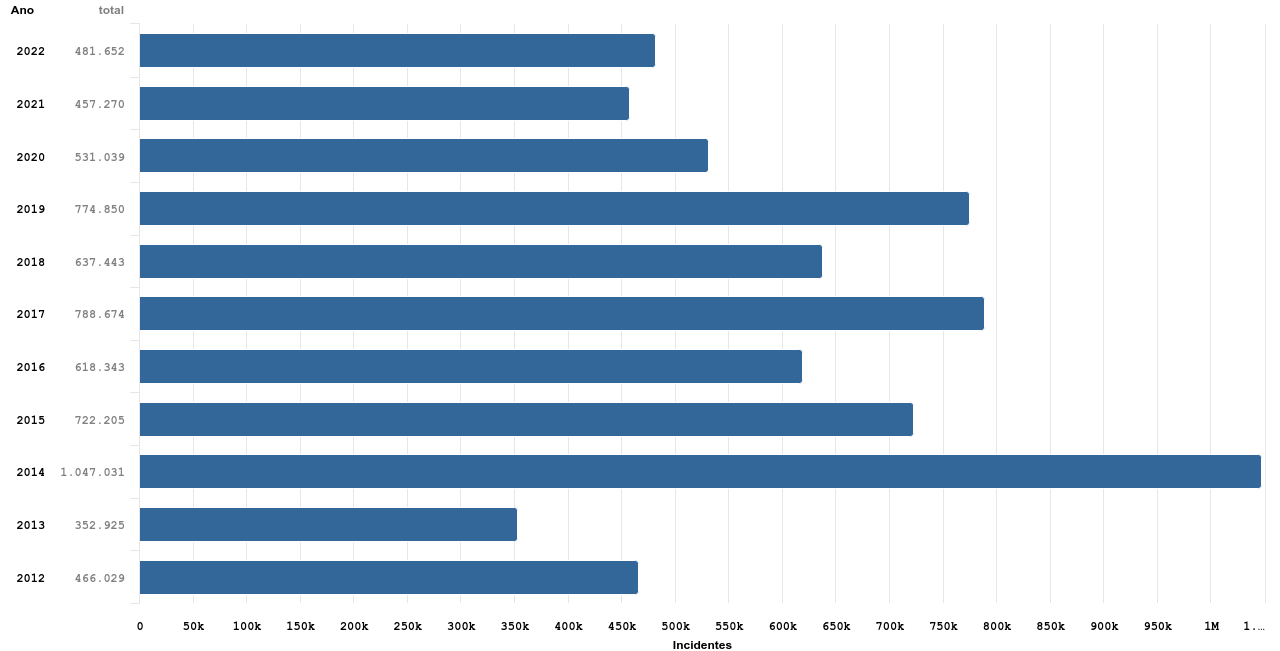
\includegraphics[width=1\textwidth]{USPSC-img/certbr.png}
        \end{center}
        \legend{Fonte: \cite{cert2023}}
    \end{figure}

    Os ataques podem ser classificados de diversas formas. A classificação base pode ser observada no glossário proposto por \citeonline{shirey2007}, cujos critérios são a origem, o destino ou alvo e objetivos do ataque. Todavia, algumas taxonomias foram propostas a fim de aprimorar essa classificação, como o modelo AVOIDIT \cite{simmons2009} -- classificando um ataque pelo seu vetor, impacto operacional, defesa, impacto informativo e alvo -- e o modelo TAVI \cite{drias2015} -- no qual divide a classificação pela \index{Ameaça Cibernética}ameaça, objetivo, \index{Vulnerabilidade}vulnerabilidade e impacto do ataque.

    Quanto à origem, os ataques podem ser externos ou internos. Os externos são aqueles disparados por um atacante de fora da rede, enquanto os internos são aqueles provenientes de usuários internos à rede que abusam de seus direitos e privilégios para realizar atividades não autorizadas \cite{turcato2020}.

    Já para a classificação com base no alvo, o ataque é realizado à rede, afetando a camada de comunicação ao impedir a utilização de alguns recursos da rede, ou ao sistema na totalidade, alterando senhas e configurações críticas dos equipamentos.
    
    No ponto de vista da classificação pelo objetivo, existem dois tipos principais de ataques que um invasor pode realizar:

    \begin{itemize}
        \item \underline{Passivo}: o intruso apenas `escuta' a comunicação, silenciosamente, sem qualquer alteração na comunicação. Tal espionagem ou análise de tráfego pode ocasionar a quebra da confidencialidade da informação, consistindo assim em crime contra a privacidade;
        \item \underline{Ativo}: refere-se à modificação de mensagens e fluxo de dados reais ou geração de dados falsos na comunicação. Afeta a integridade e confidencialidade dos dados, uma vez que o intruso pode repetir fluxos de dados antigos, alterando as mensagens de comunicação ou removendo alguma parte selecionada de mensagens importantes de comunicação. Os ataques ativos mais frequentes a redes posem ser classificados como: R2L (\textit{Remote to Local}) e U2R (\textit{User to Root}).
    \end{itemize}

    O \textit{Sniffing} de pacotes representa um ataque passivo em relação ao objetivo, uma vez que não envolve a modificação ou interrupção direta do tráfego de rede. Consiste em uma técnica aplicada para a captura e inspeção minuciosa dos pacotes em uma conexão estabelecida, sem que os agentes da comunicação estejam cientes da interceptação. Vale ressaltar que, enquanto o \textit{Sniffing} em si não causa alterações no tráfego ou nos dados, as informações obtidas podem ser posteriormente exploradas em ataques subsequentes. Por outro lado, o ataque \textit{Probing} é realizado de forma ativa, apesar de não comprometer o sistema. Envolve uma varredura do mesmo por parte do invasor pelo envio de requisições ao alvo, visando identificar entradas do sistema ou \index{Vulnerabilidade}vulnerabilidades para posteriormente explorar as fraquezas encontradas.
    
    No ataque DoS, uma sobrecarga do sistema ou rede é ocasionada por meio de solicitações excessivas do invasor, resultando em um esgotamento dos recursos computacionais ou de memória dos equipamentos. Com isso, os componentes da rede ficam impossibilitados de executarem suas tarefas devido ao envio de uma quantidade de informações superior ao que o sistema possa manipular (\textit{flooding}), assim como algumas \index{Vulnerabilidade}vulnerabilidades podem ser expostas a partir desse tipo de ataque ativo (exploração de falhas). Há a possibilidade desse ataque ser realizado em série, cujos invasores utilizam de vários locais para lançar o ataque, classificando-o assim como DDoS (do inglês \textit{Distributed DoS}). Um exemplo de DoS no âmbito industrial é um cujo invasor envia um comando para desligar a CPU de um CLP, exigindo a execução de um \textit{hard-reset} do dispositivo para retorno. Uma vez desligada, o CLP não pode se comunicar ou processar qualquer informação, resultando em uma `negação de serviço'.

    Quando ocorre a obtenção não autorizada de dados confidenciais de comunicação, caracteriza-se um ataque do tipo \textit{Man-In-The-Middle} (MITM), também conhecido como "Espionagem" (do inglês \textit{Eavesdropping}). Essa ação maliciosa pode resultar em uma significativa violação de segurança ou no comprometimento das informações, o que, por sua vez, pode abrir caminho para ataques subsequentes. Em um cenário Cliente-Servidor, caso o invasor já tenha comprometido o canal de comunicação, ele tem a capacidade de gravar e capturar as mensagens, afetando assim a confidencialidade dos dados. Além disso, uma vez estabelecida a sessão, tanto a autorização quanto a autenticação podem ser impactadas.

    Nos ataques de penetração, conhecidos como R2L e U2R, aquisições ou alteração não autorizada dos privilégios, recursos ou dados do sistema, violando as propriedades de integridade e controle dos recursos e dados. Com esses ataques, pode-se ganhar controle de um sistema ao explorar uma variedade de falhas de \textit{software} \cite{turcato2020}. A categoria R2L se destaca pelo envio de pacotes por uma rede externa, a fim de explorar privilégios de um usuário local. Já na U2R, os invasores conseguem acesso na rede local, e nesse cenário, tenta explorar as \index{Vulnerabilidade}vulnerabilidades para obter privilégios adicionais.

    % As características, a complexidade e a crescente sofisticação dos ataques faz com que aumente a demanda por técnicas de detecção mais precisas para o monitoramento contínuo da rede de comunicação industrial. Tais técnicas devem ser capazes de lidar com novos tipos de ataques e integrar-se facilmente aos demais mecanismos de proteção da rede sem sobrecarregar a comunicação \cite{maglaras2014}.

    De acordo com \cite{cekerevac2017}, o ataque MITM e DoS são os tipos mais comuns de ataque que a IIoT enfrenta, sendo responsáveis por quase 64\% dos ataques. Com o aumento da interconectividade entre sistemas nas indústrias, o ataque MITM está se tornando um desafio maior, pois é mais fácil para o invasor obter acesso a informações confidenciais através dele. Quando se trata de DoS, além de ser também comumente empregado, pode agir de maneira ativa no sistema, gerando perdas consideráveis para as indústrias. Neste projeto, três ataques são aplicados em uma rede industrial OPC UA: \textit{sniffing} de pacotes, MITM e DoS.
    
    % \subsection{Modelagem de Ameaças} \label{subsec:modAmeaca}

    \subsection{Análise e Descoberta de Vulnerabilidades} \label{subsec:analVul}

    Inúmeros empreendimentos de pesquisa têm sido dedicados à análise das origens de erros presentes em sistemas computacionais e \textit{softwares} (popularmente denominados \textit{bugs}). Visando a minimização das ocorrências desses erros nos sistemas e o desenvolvimento de métodos para avaliar a existência, esses estudos apresentam, ordinariamente, ferramentas para a identificação de \textit{bugs} específicos.

    Apesar da implementação de várias técnicas e tecnologias, esses erros intrínsecos ao desenvolvimento persistem. As vulnerabilidades surgem quando os \textit{bugs} comprometem a integridade do sistema ou políticas de segurança, podendo ser mensurada pelo grau em que um sistema, subsistema ou componente do sistema tem probabilidade de sofrer danos devido à exposição a um perigo.

    As vulnerabilidades podem ser amplamente difundidas e consistentes em vários sistemas. Erros de desenvolvimento, equívocos de configuração e falhas operacionais, frequentemente, servem como porta de entrada para usuários não autorizados, permitindo que efetuem ações maliciosas: expor/alterar informações confidenciais, interromper/destruir um sistema ou assumir o controle de um sistema/\textit{software} \cite{dowd2006}. Um estudo realizado por \citeonline{shin2022} revela que 92\% dos sistemas que utilizam o protocolo OPC UA estão inadequadamente configurados devido a diversas falhas, como a ausência de controle de acesso, a desativação de funcionalidades de segurança, a utilização de políticas criptográficas obsoletas e a reutilização de certificados. Essa alta porcentagem de inadequações é atribuída principalmente à complexidade das configurações de segurança intrínsecas ao protocolo.
    
    A análise de vulnerabilidades engloba a formulação de uma categorização, ou conjunto destas, que viabiliza a extração das informações pertinentes de um conjunto de vulnerabilidades. De acordo com \citeonline{bishop1999}, essas informações podem abranger um conjunto de assinaturas, visando a detecção de intrusões; um conjunto de condições ambientais necessárias para que um invasor explore a vulnerabilidade; um conjunto de características de codificação que facilitem a interpretação do código; ou outras formas de dados. Logo, os dados específicos utilizados para classificar as vulnerabilidades variam conforme os objetivos particulares da categorização, sustentando, assim, a existência de diversos esquemas de classificação.

    Com base na indecidibilidade do Problema da Parada de Turing e no Teorema de Rice, é possível demonstrar que muitos problemas relacionados à análise de vulnerabilidades também são indecidíveis em um contexto amplo \cite{ghaffarian2017}. Isso resulta na falta de uma solução abrangente e definitiva para esses problemas práticos.

    Na matemática, um sistema de prova é considerado válido quando não aceita argumentos inválidos e é completo quando aceita todos os argumentos válidos. Da mesma forma, na segurança de \textit{software}, um método de análise de vulnerabilidades é apontado sólido se não aprova sistemas vulneráveis. Caso consiga aprovar todos os programas seguros, sem detectar vulnerabilidades falsas, considera-o completo. Comparativamente, a descoberta de vulnerabilidades de programas oferece informações mais detalhadas sobre cada vulnerabilidade em um programa específico.

    Embora o problema da análise e descoberta de vulnerabilidades seja indecidível, a comunidade acadêmica e a indústria de \textit{software} têm proposto várias abordagens devido à sua importância crítica. Essas abordagens, no entanto, são aproximações que frequentemente carecem de solidez ou completude. Assim, a pesquisa busca melhorias específicas em várias áreas, como cobertura de vulnerabilidades, precisão de descoberta e eficiência de execução.

    No entanto, apesar dos desafios inerentes à classificação de vulnerabilidades, as abordagens de análise de vulnerabilidade no âmbito de \textit{software} podem ser categorizadas em três principais vertentes, segundo \citeonline{ghaffarian2017}:

    \begin{itemize}
        \item \underline{Análise Estática}: a análise é realizada com base no código-fonte do \textit{software}, sem a necessidade de execução. Uma abstração generalizada é necessária para avaliar as propriedades do mesmo, concedendo a essa abordagem a capacidade de ser sólida. Porém, caso não haja precisão na generalização, a análise pode resultar em falsas vulnerabilidades. Por isso, deve-se encontrar um equilíbrio entre a precisão e a eficiência computacional;
        \item \underline{Análise Dinâmica}: um programa é avaliado enquanto é executado com dados de entrada específicos, monitorando seu comportamento em estados. No entanto, devido à natureza das entradas e esses estados de tempo de execução, sistemas de análise dinâmica não conseguem conceituar completamente o comportamento do \textit{software}. Assim, podem ser completos, aprovando todos os programas seguros e não reportando vulnerabilidades falsas, mas não podem ser sólidos, pois existe a possibilidade de negligenciar vulnerabilidades em estados invisíveis. Limitações práticas incluem a necessidade de um ambiente de tempo de execução funcional e o processamento demorado para casos de teste em \textit{software} complexo;
        \item \underline{Análise Híbrida}: combina técnicas de análise estática e dinâmica. Embora possa parecer que a abordagem híbrida une as vantagens de ambas, sendo sólida e completa, isso não é verdade, pois enfrentam também suas limitações. Pode ser uma análise estática com análise dinâmica para identificar vulnerabilidades falsas ou uma análise dinâmica que utiliza técnicas estáticas para orientar a seleção e análise de casos de teste.
    \end{itemize}

    Vale ressaltar que nem todos os sistemas de análise estática são sólidos e nem todos os sistemas de análise dinâmica são completos.
    
    De acordo com \citeonline{ghaffarian2017}, entre as diversas abordagens de descoberta de vulnerabilidades, algumas já estão bem estabelecidas na indústria de \textit{software}; a saber:

    \begin{itemize}
        \item \underline{Teste de Penetração}: envolve um teste manual de segurança realizado por uma equipe de especialistas em segurança, que exploram as vulnerabilidades em busca de possíveis pontos de entrada para invasões;
        \item \underline{\textit{Fuzz-Testing}}: também conhecido como teste aleatório, os dados de entrada válidos são aleatoriamente alterados e inseridos na execução em teste, enquanto as falhas são monitoradas para identificar possíveis vulnerabilidades;
        \item \underline{Análise Estática de Fluxo de Dados}: também referida como "Análise de Fluxo de Dados Contaminado", é uma abordagem de análise estática em que dados de entradas de fontes não confiáveis são classificados como contaminados. Seu fluxo em direção a instruções confidenciais do \textit{sofware} é rastreado como um possível indicador de vulnerabilidade.
    \end{itemize}

    {\color{red}
    \section{Indicadores de Desempenho em Redes Industriais}

    A análise do tráfego de rede em sistemas industriais, como aqueles baseados no protocolo OPC UA, requer a utilização de diversos indicadores de desempenho para avaliar a eficácia e a segurança da comunicação. Dois desses indicadores cruciais são o throughput e o round trip time (RTT). A seguir, são definidas e discutidas suas importâncias e aplicações no contexto de redes industriais.

    {\color{red}O throughput é uma medida crítica da capacidade de transmissão de dados da rede. A análise do throughput permite identificar como os ataques afetam a quantidade de dados que podem ser transmitidos em um determinado período. Reduções significativas no throughput indicam que o ataque está conseguindo interromper ou diminuir a eficiência da comunicação na rede. Este indicador é essencial para avaliar a degradação da performance da rede e a eficácia das políticas de segurança implementadas.

    O desempenho da RAM e da CPU é um indicador direto da carga de trabalho imposta ao servidor OPC UA durante um ataque. Monitorar o uso desses recursos é crucial para identificar sobrecargas que podem levar à instabilidade ou falhas no sistema. Um aumento significativo no uso de CPU e RAM durante um ataque pode sugerir que o servidor está sendo sobrecarregado com solicitações maliciosas, o que pode comprometer sua capacidade de atender às solicitações legítimas. Analisar esses dados ajuda a entender a resistência do servidor sob diferentes tipos de ataques e políticas de segurança.

    A quantidade de pacotes OPC UA por segundo fornece uma visão detalhada do fluxo de dados na rede. Alterações abruptas na quantidade de pacotes podem indicar comportamentos anômalos ou interrupções causadas pelos ataques. Este indicador é especialmente útil para detectar atividades suspeitas, como tentativas de captura de dados (sniffing) ou interferências na comunicação (MITM). A análise desse gráfico ajuda a identificar padrões de tráfego anômalos que podem estar associados a atividades maliciosas.

    O RTT normalizado é uma medida da latência na comunicação entre cliente e servidor. A latência é um fator crítico para a eficiência e a responsividade das redes OPC UA. Aumentos no RTT durante um ataque indicam que a comunicação está sendo retardada, possivelmente devido a sobrecargas ou interferências. Analisar o RTT ajuda a entender como os ataques afetam a velocidade e a eficiência da comunicação na rede, e a normalização permite comparar o impacto em diferentes cenários de forma consistente.

    A representação visual dos dados através dos gráficos permite uma interpretação mais intuitiva e imediata dos impactos dos ataques. Gráficos fornecem uma forma eficaz de identificar tendências, anomalias e padrões que podem não ser facilmente detectáveis através da análise de dados brutos. Além disso, eles facilitam a comparação entre diferentes cenários de ataque e políticas de segurança, permitindo uma avaliação clara da eficácia das medidas de proteção implementadas.

    Em resumo, a análise dos gráficos de throughput, desempenho de RAM e CPU, quantidade de pacotes por segundo e RTT normalizado oferece uma compreensão detalhada e multidimensional dos efeitos dos ataques cibernéticos em redes OPC UA. Essa abordagem é essencial para identificar vulnerabilidades, avaliar a eficácia das políticas de segurança e desenvolver estratégias de defesa mais robustas.}

    \subsection{Throughput}

    O throughput é um indicador de desempenho que mede a quantidade de dados transmitidos através da rede em um período específico, geralmente expresso em kilobits por segundo (kbps) ou megabits por segundo (Mbps). Ele é um parâmetro fundamental para avaliar a capacidade e eficiência de uma rede em transportar dados.

    A análise do throughput em redes OPC UA é vital por várias razões:

    \begin{enumerate}
        \item \textbf{Capacidade da Rede:} Avaliar o throughput permite determinar se a rede pode suportar a quantidade de dados necessária para a operação contínua e eficiente de sistemas industriais.
        \item \textbf{Detecção de Gargalos:} Um throughput baixo pode indicar gargalos ou problemas de congestionamento na rede, que podem afetar a performance geral dos sistemas de controle e automação.
        \item \textbf{Impacto de Ataques:} Durante ataques cibernéticos, como DoS, o throughput pode ser significativamente afetado. Analisar as mudanças no throughput pode ajudar a identificar a presença e a intensidade de tais ataques.
    \end{enumerate}

    Para medir o throughput, são utilizados softwares de monitoramento de rede que capturam e analisam pacotes de dados transmitidos. Em nosso estudo, o throughput foi calculado durante um período de 60 segundos para cada cenário de ataque, sob diferentes políticas de segurança do OPC UA.

    \subsection{Round Trip Time (RTT)}

    O round trip time (RTT) é o tempo que um pacote de dados leva para ir do ponto de origem ao destino e voltar ao ponto de origem. É um indicador crucial da latência de rede e é normalmente medido em milissegundos (ms).

    A importância do RTT na análise de desempenho de redes industriais OPC UA inclui:

    \begin{enumerate}
        \item \textbf{Latência de Comunicação:} O RTT oferece uma medida direta da latência na comunicação entre dispositivos. Em sistemas de controle industrial, uma latência baixa é essencial para o funcionamento em tempo real.
        \item \textbf{Qualidade de Serviço:} Um RTT elevado pode indicar problemas na rede que impactam negativamente a qualidade do serviço (QoS), como roteamento ineficiente, problemas de congestionamento, ou ataques cibernéticos.
        \item \textbf{Detecção de Anomalias:} Análises de RTT podem ajudar a identificar anomalias na rede, como atrasos inesperados que podem ser causados por problemas de configuração ou atividades maliciosas.
    \end{enumerate}

    A medição do RTT envolve a análise do tempo de ida e volta de pacotes de dados utilizando ferramentas de rede. Em nossa pesquisa, o RTT foi normalizado em uma escala de 0 a 1 e analisado para cada cenário de ataque, proporcionando uma visão detalhada das variações na latência sob diferentes condições de segurança.
    }

    \section{Trabalhos Correlatos} \label{sec:trabCorrelatos}

    O crescente dinamismo dos sistemas industriais e o aumento significativo dos ataques aos IACSs demandam estudos aprofundados para compreender como as mudanças na arquitetura desses sistemas afetam o desempenho dos mecanismos de segurança. Além disso, é fundamental manter constantemente atualizada a base de conhecimento, particularmente no que diz respeito aos principais aspectos de segurança cibernética relacionados ao protocolo OPC UA, amplamente utilizado por esses sistemas industriais.

    \citeonline{matrikon2019} destacam a crescente importância de estabelecer uma segurança sólida entre a TI e TO à medida que a digitalização se expande. Embora ambas tecnologias busquem uma comunicação segura, ressalta-se que suas abordagens são distintas. Enquanto a TO prioriza eficiência, consistência e continuidade, a TI se concentra em segurança e flexibilidade. Logo, a solução do protocolo OPC UA é proposta, originalmente introduzido pelo setor de TO, mas visando abranger todos os parâmetros de segurança da TI. Além disso, destaca-se o foco do OPC UA na proteção do canal de comunicação, fundamental para a transformação segura de informações confidenciais, concentrando-se no conceito de \textit{Data In Motion}. Adicionalmente, a segurança das implantações OPC UA foi avaliada por \citeonline{roepert2020} e \citeonline{polge2019}, cujo relato garante um alto nível de segurança do protocolo, desde que sejam realizadas as configurações de segurança corretas.

    A extensa análise bibliográfica realizada no trabalho sobre o protocolo \index{OPC UA}OPC UA, resultou em uma gama de publicações concernentes à segurança do protocolo. Em \cite{luo2020}, é discutida a importância da segurança na automação industrial e as \index{Vulnerabilidade}vulnerabilidades das redes de comunicação \index{OPC UA}OPC UA e proposto um método de criptografia de segurança baseado no algoritmo \textit{Advanced Encryption Standard} (AES). \citeonline{kohnhauser2021} complementam a discussão acima mencionada com a importância do provisionamento seguro em \index{IIoT}IIoT, bem como \cite{kohnhauser2022} para os dispositivos \index{IIoT}IIoT usando \index{OPC UA}OPC UA. \citeonline{muhlbauer2020} projetam uma implementação de código aberto do \index{OPC UA}OPC UA para melhorar a segurança e a escalabilidade na automação industrial.

    O estudo sobre a segurança do OPC UA realizado pelo Escritório Federal Alemão para Segurança da Informação \cite{bsi2017} analisa as principais vulnerabilidades e possíveis ameaças dessas redes, baseando-se no tipo de mensagem e modo de segurança escolhido. No entanto, a maioria dos ataques são somente efetuados nos modos de segurança \textbf{None} e \textbf{Sign}, diferentemente do presente trabalho, nas quais as conexões são também estabelecidas no modo \textbf{Sign\&Encypt}.

    Uma análise detalhada sobre ataques de negação de serviço em redes \index{OPC UA}OPC UA é realizada por \citeonline{neu2019}. Nesse contexto, uma abordagem para detectar tais ataques nesse tipo de rede é implementada, apresentando como esses ataques podem afetar o consumo de CPU do servidor e podem ser muito poderosos quando inúmeros dispositivos é comprometido.

    O estudo \cite{kaspersky2018} aponta que a maioria das vulnerabilidades de segurança do protocolo OPC UA, identificadas por meio de testes de \textit{fuzzing}, decorre de produtos e bibliotecas que não estão em conformidade com as especificações. Nessa circunstância, foram identificadas 17 vulnerabilidades de segurança em produtos relacionados à OPC UA. Por sua vez, \citeonline{puys2016} revisam as propriedades de confidencialidade e autenticação por meio do uso da ferramenta de verificação de protocolos de criptografia ProVerif. Constatou-se que esses requisitos da segurança são atendidos quando se utiliza o modo de assinatura e criptografia.

    Em \cite{varadarajan2022}, três principais ciberataques que ocorrem na IIoT são efetuados em redes OPC UA: \textit{packet sniffing}, \textit{Man-in-the-Middle} (MITM) e negação de serviço (DoS). Um cenário de ataque foi construído e testes de penetração foram realizados por meio de simulações de ataque cibernético que podem ocorrer em uma configuração de segurança inadequada.

    Além disso, \citeonline{hildebrandt2020} demonstraram que um ataque de injeção de comando por meio de um canal oculto pode ser realizado em um pacote transmitido de um servidor para um cliente em um ambiente de comunicação baseado no protocolo OPC UA, representando uma potencial ameaça à cadeia de suprimentos.
    
    \citeonline{polge2019} identificaram novas ameaças que podem ocorrer usando o protocolo OPC UA com base em um modelo de ameaças de segurança IoT. O ataque identificado a partir de seu modelo de ameaças OPC UA proposto verificou a possibilidade de dois tipos de ataques de negação de serviço (DoS), utilizando MITM e ataques de inundação.

    \citeonline{shin2022} propõem um framework para a descoberta de vulnerabilidades e contramedidas, utilizando o protocolo OPC UA, mas que pode ser aplicado a qualquer alvo de análise. Um teste de conceito é conduzido para derivar e verificar ameaças que podem efetivamente ocorrer por meio da modelagem de ameaças abordadas neste trabalho. Com base no framework proposto, foram identificadas 30 ameaças significativas e quatro vulnerabilidades. Como resultado, a validade de ataques de clientes maliciosos usando certificados e cenários de ataque de negação de serviço (DoS) por inundação foi comprovada, e contramedidas foram desenvolvidas para essas vulnerabilidades.

\chapter{Desenvolvimento} \label{cap:desenvolvimento}

Devido à importância do tema e ao raciocínio apresentado, um método para análise de \index{Vulnerabilidade}vulnerabilidades em redes industriais \index{OPC UA}OPC UA foi desenvolvido. O presente capítulo oferece os principais aspectos da bancada experimental utilizada e o conjunto de estratégias adotados para a realização e desenvolvimento do mesmo.

\section{Aspectos da Bancada Experimental para Ensaios de Intrusão em Redes OPC UA}

    Nesta seção, toda a estrutura responsável pela aquisição de dados experimentais gerados para auxiliar no desenvolvimento do trabalho é descrita. A \autoref{fig:esqBanc} ilustra a composição da estrutura da bancada experimental utilizada, cujos principais componentes são detalhados a seguir:

    \begin{figure}[htbp]
        \caption{\label{fig:esqBanc}Esquema geral da bancada experimental para ensaios de segurança cibernética}
        \begin{center}
            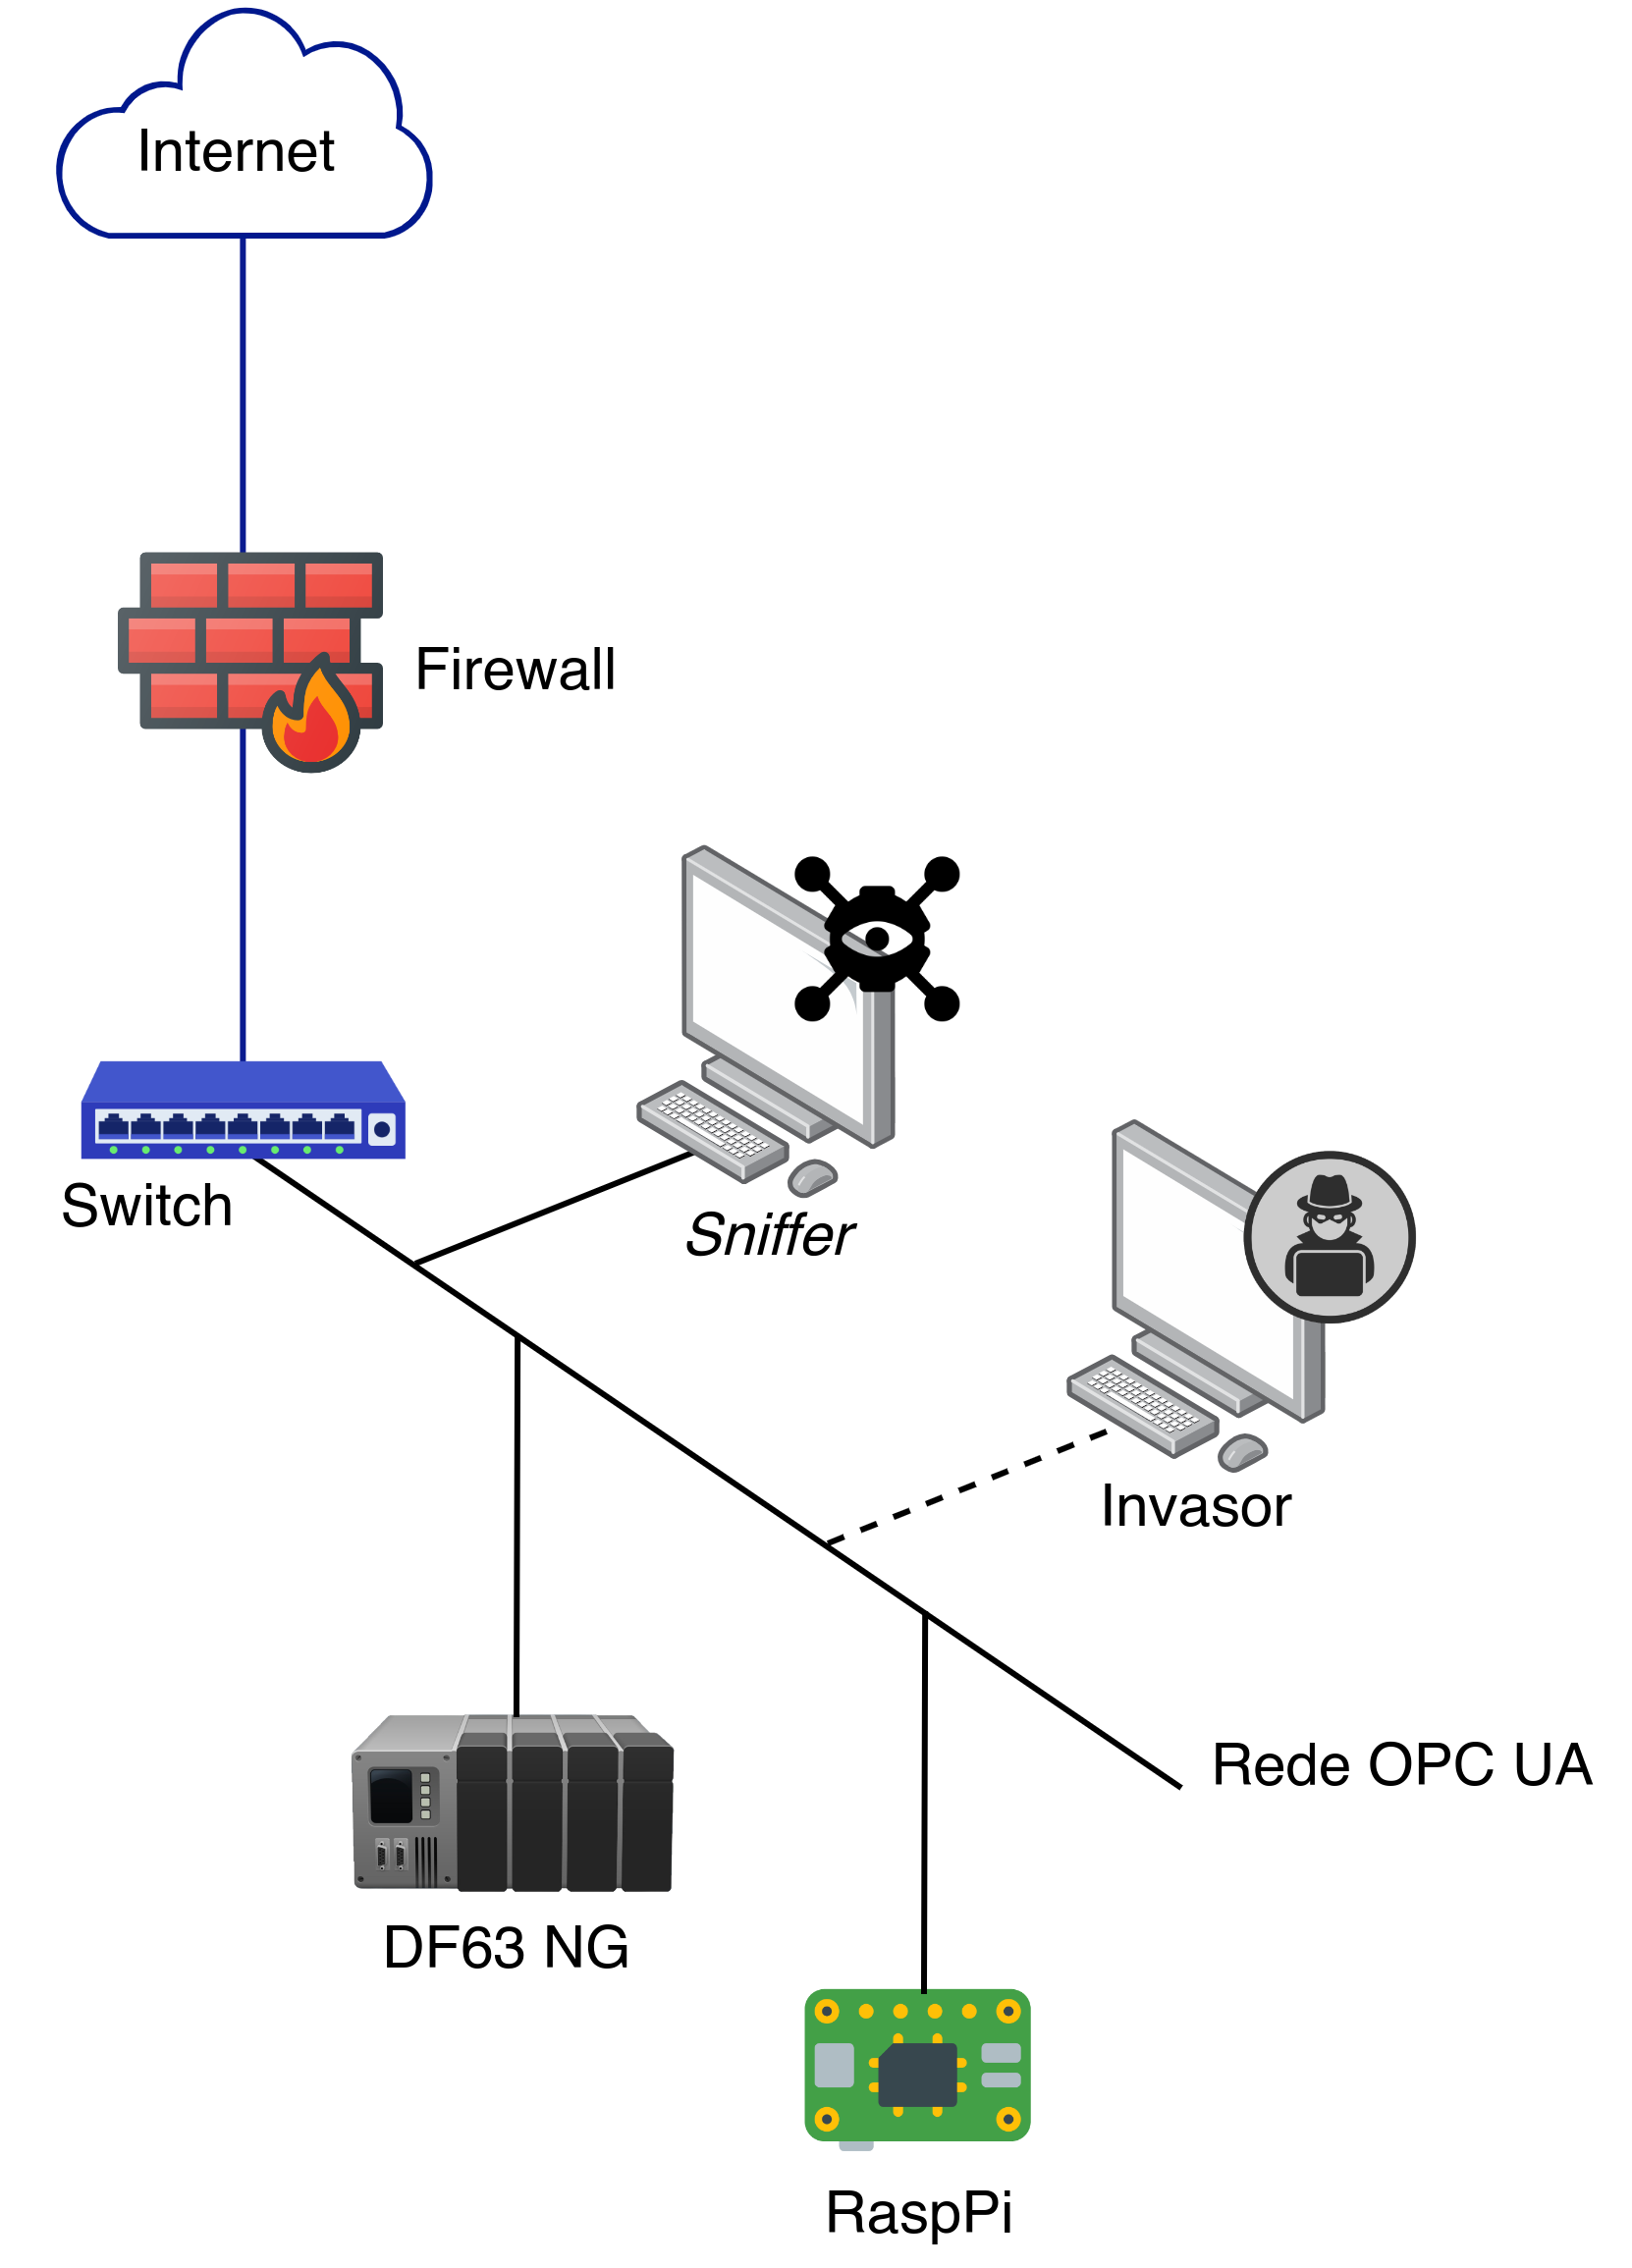
\includegraphics[width=0.6\textwidth]{USPSC-img/bancada.png}
        \end{center}
        \legend{Fonte: elaborada pelo autor.}
    \end{figure}

    \subsection{\textit{Hardware}}

    Para simular os ataques cibernéticos, são necessários um conjunto de componentes de \textit{hardware} combinados com ferramentas de \textit{software} específicas. A lista a seguir detalha cada equipamento utilizado.

    \begin{itemize}
        \item \underline{DF63 NG}: representa a nova geração dos controladores multifuncionais da plataforma DFI302 da Nova Smar S/A funcionando como um `\textit{linking device}' para conectar redes H1 independentes e redes Ethernet HSE, especialmente projetado para soluções de controle distribuído em redes industriais. Além de suportar comunicação Modbus, oferece recursos avançados, incluindo redundância `\textit{Hot standby}', comunicação OPC UA nativa, estampa de tempo e configuração por meio da linguagem Ladder conforme IEC 61131. A DF63 NG é altamente versátil, permitindo a instanciação de centenas de blocos funcionais, incluindo blocos flexíveis, e possui um servidor Web integrado para diagnóstico e parametrização;
        \item \underline{Raspberry Pi 4 Modelo B}: são utilizados dois mini-computadores de placa única multiplataforma, configuradas com o sistema operacional Kali Linux, hospedando um cliente e um servidor OPC UA cada. A Raspberry Pi 4 Modelo B representa uma evolução significativa em relação às gerações anteriores, incorporando um processador ARM Cortex-A72 quad-core de 64 bits rodando a 1,5 GHz, suporte a Wi-Fi 802.11ac, Bluetooth 5.0 e maior capacidade de memória. Estes aprimoramentos garantem um ambiente experimental mais robusto e capacidade de processamento aprimorada para a condução de testes de intrusão em redes OPC UA. Todas as Raspberry Pi's existentes na bancada experimental são configuradas como cliente e servidor OPC UA;
        \item \underline{Ethernet Switch}: Trata-se de um dos dispositivos de rede mais ubíquos, empregado para centralizar a comunicação entre múltiplos dispositivos. Utiliza a técnica de comutação de pacotes para receber e encaminhar dados de um dispositivo para outro. Neste projeto, faz-se uso de um \textit{Switch} Ethernet da marca TP-Link para estabelecer uma conexão entre os clientes OPC UA e o servidor. O componente de rede que atuar como hospedeiro do servidor OPC UA, encontra-se conectado ao comutador Ethernet por meio de um cabo LAN, da mesma maneira que outro responsável por hospedar o cliente também está conectado ao\textit{Switch}. Cumpre destacar que os comutadores Ethernet da TP-Link incorporam tecnologia Ethernet verde, que resulta em economia de consumo energético, enquanto o controle de fluxo IEEE 802.3x proporciona uma transferência de dados confiável.
        \item \underline{Elemento Invasor}: desempenha um papel fundamental na condução dos testes de intrusão propostos neste estudo. Representa uma simulação de ataque por meio de um computador que pode ser configurado de maneira flexível para atender a cenários específicos de teste. Os ataques são realizados utilizando uma variedade de ferramentas de software, como Hping3 e Nmap (veja \autoref{subsec:software}). Vale ressaltar que o Elemento Invasor é empregado com extrema cautela em um ambiente controlado, a fim de evitar qualquer impacto adverso e garantir a segurança contínua. Assim, respeitando rigorosamente as considerações éticas, os ataques efetuados neste trabalho pelo elemento invasor não implicam em nenhuma violação das regulamentações estabelecidas pela Lei Geral de Proteção de Dados (LGPD) por não ser aplicado em nenhuma rede ou implementação real.
    \end{itemize}
    
    \subsection{\textit{Software}} \label{subsec:software}

    Um conjunto de ferramentas de \textit{software} é necessário para conduzir os ataques às redes OPC UA, das quais se destacam:

    \begin{itemize}
        \item \underline{Smar OPC UA server}: servidor OPC UA proprietário da Nova Smar S/A, é amplamente aplicado no setor industrial juntamente com a linha de produtos compatíveis com o novo padrão O-PAS (do inglês, \textit{Open Process Automation™ Standards}), desenvolvido pelo OPAF (do inglês, \textit{Open Process Automation™ Forum}), oferecendo um ambiente altamente seguro e eficiente para a comunicação e troca de dados em sistemas de automação industrial. A Nova Smar S/A continua aprimorando seu servidor OPC UA para atender às crescentes demandas do mercado, proporcionando uma solução de conectividade sólida e confiável;
        \item \underline{opcua-asyncio}: implementação de código aberto do OPC UA, escrito em Python com suporte para asyncio. O opcua-asyncio opera sob a GNU Lesser General Public License v3.0,  permitindo sua integração e distribuição com \textit{software} proprietário. Essa biblioteca é versátil, compatível com vários ambientes Python, e oferece informações detalhadas sobre a implementação de clientes e servidor OPC UA. O opcua-asyncio implementa o conjunto de protocolos binários OPC UA, SDK de cliente e servidor, e é uma opção flexível para desenvolvedores que preferem Python como sua linguagem de programação;
        \item \underline{OPC UA Exploit Framework}: projeto \textit{open-source}, desenvolvido e mantido pela Claroty Team82, que fornece um framework avançado de ferramentas para pesquisa e exploração de vulnerabilidades em redes OPC UA. O intuito deste projeto é facilitar e auxiliar empresas desenvolvedoras de software e fornecedoras de OPC UA na fase de teste e aprimoramento dos seus produtos, além de suportar pesquisadores da área na análise de novas vulnerabilidades e \textit{bugs} sistêmicos;
        \item \underline{Ettercap}: ferramenta de \textit{software} utilizada principalmente para implementar ataques do tipo MITM. Possui recursos extras de captura de conexões \textit{real-time}, filtragem de conteúdo e análise de \textit{hosts} de destino. O Ettercap é utilizado neste projeto para implementar o primeiro cenário de ataque, capturando a conexão entre cliente e servidor OPC UA;
        \item \underline{Hping3}: ferramenta de linha de comando que serve como montadora e analisadora de pacotes TCP/IP. Inicialmente concebida para executar ataques de negação de serviço (DoS), o hping3 é agora amplamente empregado em testes de segurança de rede. Oferece suporte a protocolos TCP, UDP e ICMP, bem como um modo de rastreamento de rota;
        \item \underline{Wireshark}: software de código aberto usado para capturar e analisar pacotes e protocolos de rede. É principalmente aplicado para solução de problemas de rede, desenvolvimento e análise de protocolos de software e comunicação. Neste trabalho, é utilizado juntamente com um computador \textit{sniffer};
        \item \underline{Nmap}: ferramenta gratuita de código aberto amplamente utilizada para varredura de rede e portas. Através dela, pode-se descobrir os \textit{hosts} e serviços em uma rede dada, bem como detalhes como qual serviço está em execução em qual porta e se a porta está aberta ou fechada, entre outros. Esse resultado é alcançado ao enviar pacotes para o alvo e analisar posteriormente sua resposta.
    \end{itemize}

\section{Ataques Cibernéticos em Redes Industriais OPC UA} \label{sec:attacks}

    Nesta seção, uma análise detalhada dos cenários de ataque implementados minuciosamente no âmbito deste projeto é apresentada. A exposição abrangente engloba uma descrição passo a passo das metodologias empregadas para orquestrar três formas distintas de ciberataques: intervenção de pacotes (do inglês \textit{Packet Sniffing}), ataques do tipo MITM e de negação de serviço. Ao elucidar as complexidades destes vetores de ataque, objetiva-se proporcionar uma compreensão profunda do cenário em evolução das ameaças à cibersegurança em redes OPC UA.

    \subsection{\textit{Packet Sniffing}}

    Uma vez que a rede OPC UA esteja instalada e funcionando em seus respectivos dispositivos, o Elemento Invasor inicia o \textit{software} Ettercap e o utiliza como um \textit{sniffer} unificado para obter informações detalhadas sobre os alvos disponíveis na rede. O modo unificado do Ettercap permite a execução do ataque por uma única interface de rede. É importante observar que o Elemento Invasor deve estar configurado na mesma rede de comunicação OPC UA e conectado a uma porta do \textit{switch} gerenciável, que por sua vez, replica o tráfego de dados das outras portas (do componente cliente e servidor OPC UA), conforme ilustrado na \autoref{fig:sniffing}. 

    \begin{figure}[htbp]
        \caption{\label{fig:sniffing}Esquemático do ataque \textit{Packet Sniffing}}
        \begin{center}
            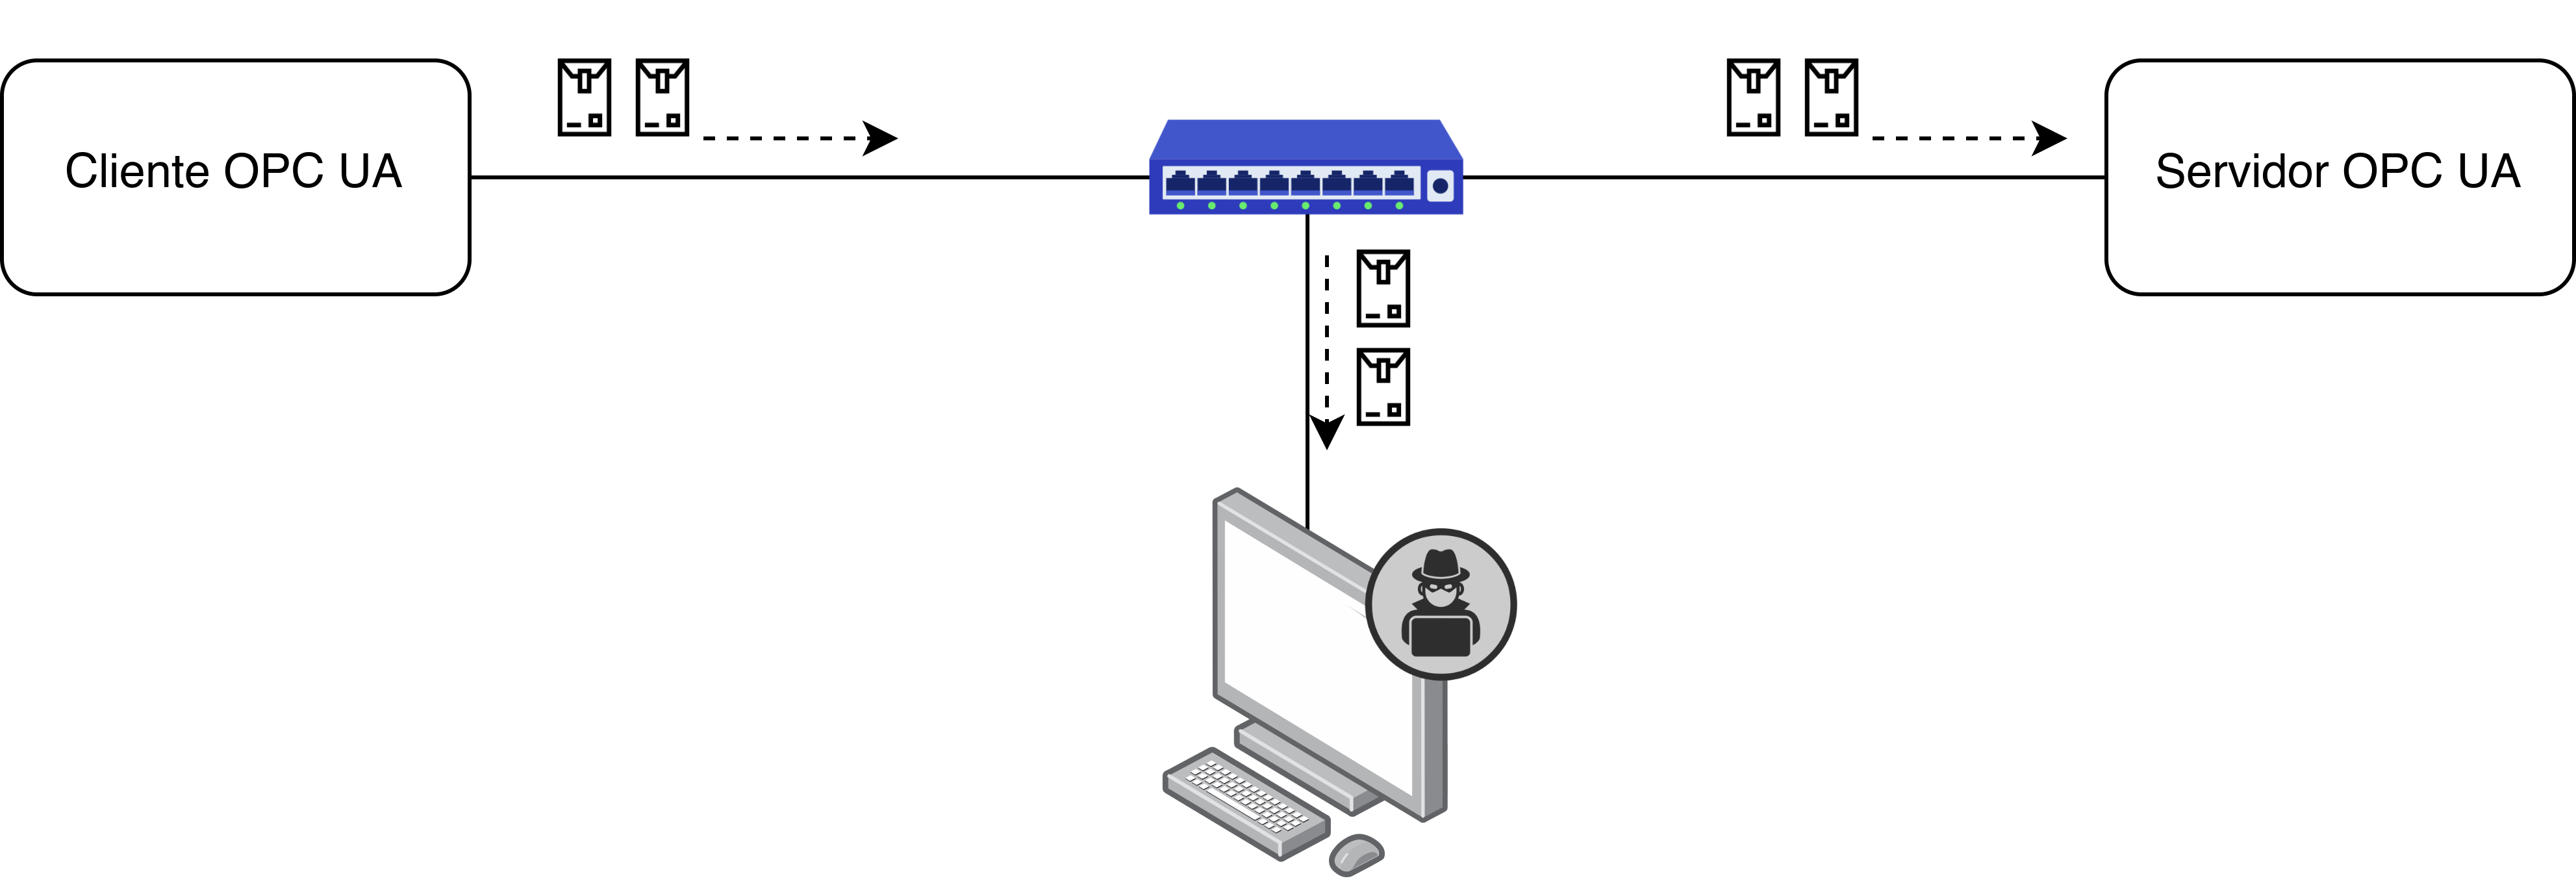
\includegraphics[width=0.9\textwidth]{USPSC-img/sniffing.png}
        \end{center}
        \legend{Fonte: elaborada pelo autor.}
    \end{figure}
    
    Com o \textit{sniffing} de rede iniciado pelo Ettercap, utiliza-se o Wireshark para analisar mais detalhes sobre os endereços obtidos. A \autoref{fig:sniffWire} apresenta a série de pacotes que o \textit{software} disponibiliza quando a operação de \textit{sniffing} do tráfego de rede é bem-sucedida. Maiores detalhes da análise aplicada nos dados obtidos nesse processo são apresentados no \autoref{cap:resultados}.

    \begin{figure}[htbp]
        \caption{\label{fig:sniffWire}Resultados de captura do Wireshark durante o \textit{sniffing} de pacotes}
        \begin{center}
            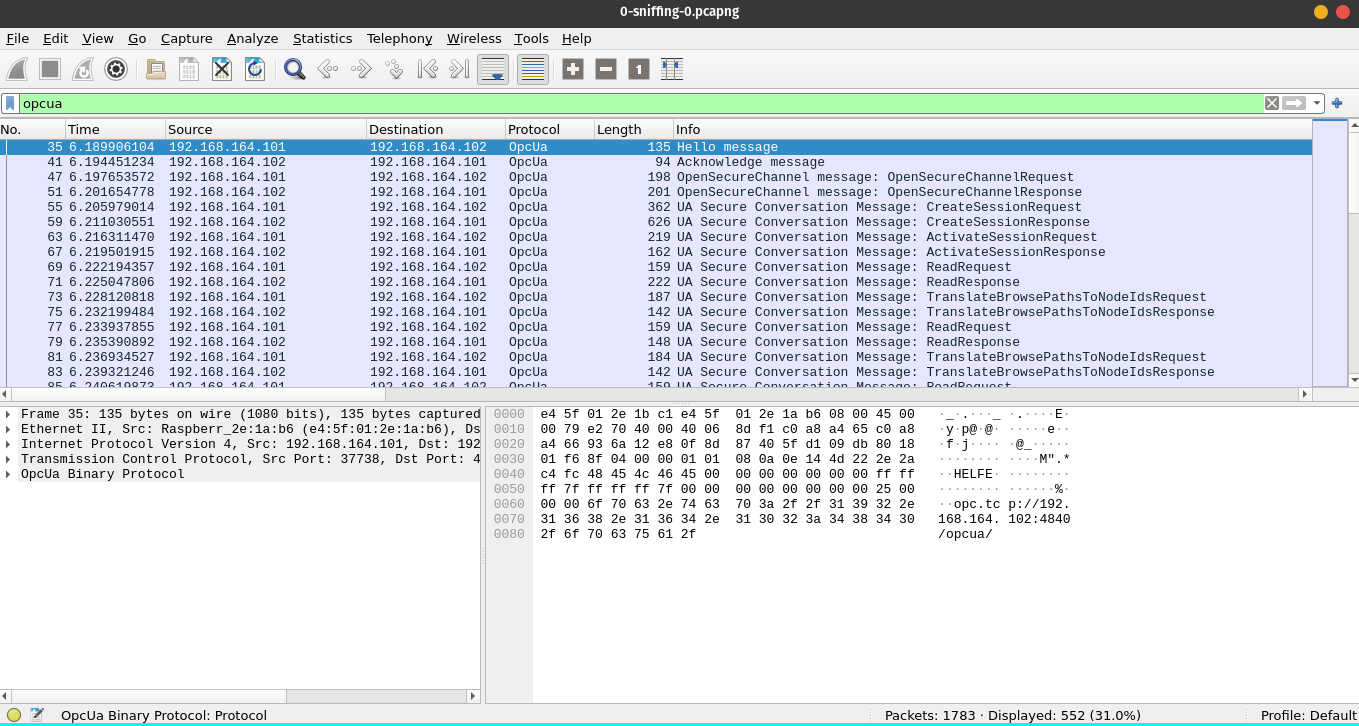
\includegraphics[width=1\textwidth]{USPSC-img/sniffWire.png}
        \end{center}
        \legend{Fonte: elaborada pelo autor.}
    \end{figure}
    
    Os detalhes dos pacotes capturados pelo Wireshark são analisados e descritos detalhadamente no \autoref{cap:resultados}.
    
    \subsection{\textit{Man in the Middle (MITM)}}

    Ao efetuar esse ataque, o Elemento Invasor pode interceptar as informações do \textbf{SecureChannel} entre o cliente e servidor OPC UA, como mostra a \autoref{fig:mitm}.

    \begin{figure}[htbp]
        \caption{\label{fig:mitm}Esquemático do ataque MITM}
        \begin{center}
            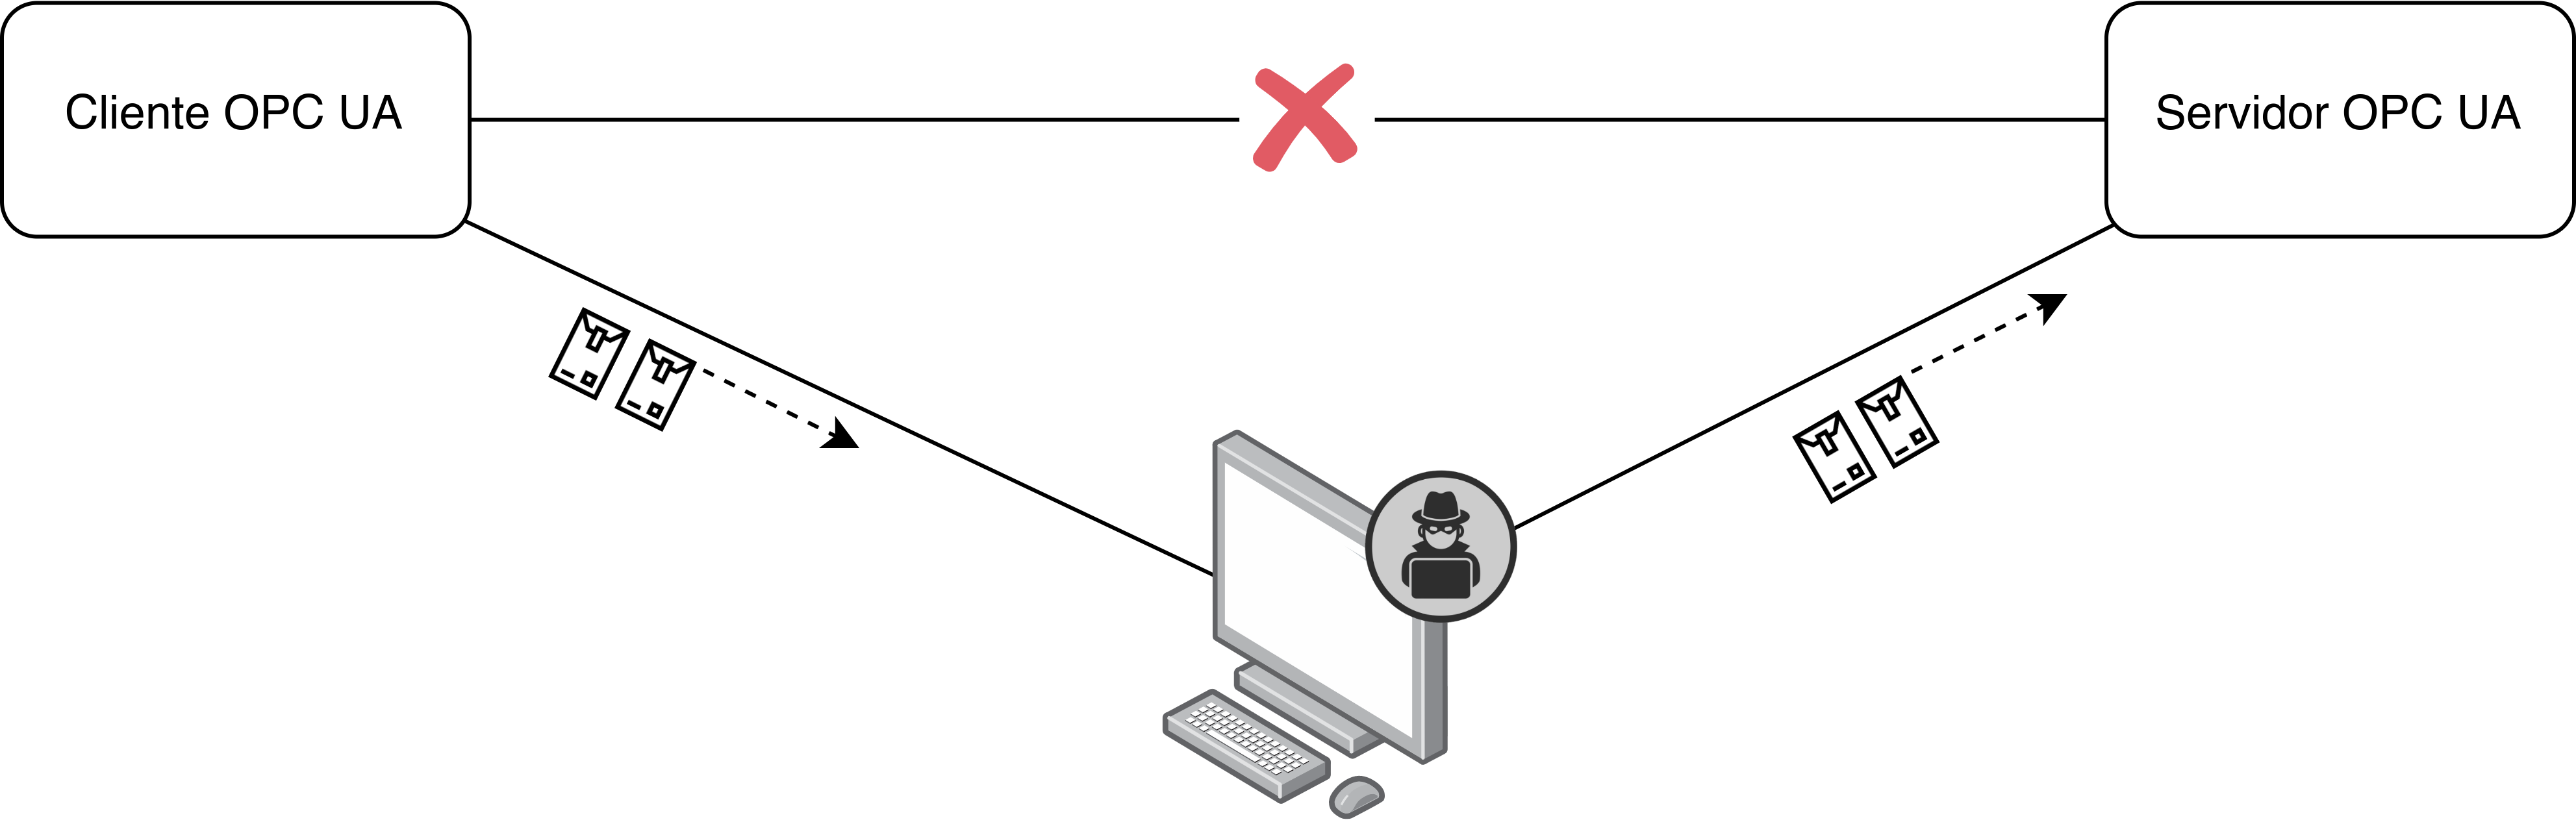
\includegraphics[width=0.9\textwidth]{USPSC-img/mitm.png}
        \end{center}
        \legend{Fonte: elaborada pelo autor.}
    \end{figure}
    
    A primeira ferramenta de software utilizada nesse processo é a Ettercap, utilizada para realizar uma varredura da rede. Ao iniciar a busca direta por \textit{hosts} ativos, todos os endereços da máscara de rede são verificados a fim de identificar quais deles estão em funcionamento. Como exemplo, caso a máscara de rede configurada seja 255.255.255.0 (24), um total de 256 endereços são varridos.
    
    Após o término dessa operação de varredura, o Elemento Invasor pode selecionar o(s) alvo(s) nos quais receberam o ataque MITM e então, prosseguir com a falsificação da rede por ARP (do inglês \textit{ARP Spoofing}), um dos tipos mais comuns de efetuar esse ataque. O ARP (do ingês \textit{Address Resolution Protocol}) é um dos protocolos de comunicação mais importantes da camada de rede do modelo OSI, utilizado para determinar o endereço MAC (do inglês \textit{Media Access Control}) de um dispositivo com base no seu endereço IP. Com o \textit{ARP Spoofing}, o invasor é capaz de anunciar à rede que o seu endereço MAC é o correto para os endereços IP pertencentes ao roteador e à estação de trabalho. Assim, estes dois dispositivos atualizam as suas entradas de cache ARP, e, a partir desse ponto, comunicam-se com o invasor, em vez de diretamente entre si.

    Além disso, realizou-se também o ataque MITM por roubo de portas (do inglês \textit{port stealing}) com a ferramenta Ettercap. Neste cenário, o invasor intercepta o tráfego de rede entre o cliente e o servidor OPC UA ao inundar a rede com pacotes ARP, cujo o endereço MAC de destino é o do próprio invasor e o endereço MAC de origem é o de uma vítima. Com isso, a porta do switch do alvo é ``roubado'', permitindo que os pacotes destinados a ela sejam recebidos pelo invasor. O invasor então interrompe a inundação, realiza uma solicitação ARP para o destino real do pacote e, ao receber a resposta, reenvia o pacote para o destino. O processo é repetido para interceptar continuamente o tráfego.

    Enquanto os ataques MITM pela falsificação da tabela ARP e pelo roubo de portas são realizados pela ferramenta Ettercap, inicia-se a captura de pacotes pelo Wireshark. Para facilitar a visualização e a análise realizada neste estudo, o Wireshark é configurado para o protocolo OPC UA, permitindo um exame detalhado da comunicação entre os dispositivos na rede.
    
    \subsection{\textit{Denial of Service (DoS)}}

    Esse tipo de ataque possibilita a inserção de clientes não confiáveis na rede OPC UA pelo Elemento Invasor, assim como uma inundação da rede e do servidor ao enviar mensagens específicas continuamente. A \autoref{fig:dos} apresenta um esquemático básico de um funcionamento de DoS, nas quais as solicitações advindas de um cliente OPC UA não confiável são interpretadas pelo servidor, mas não são aceitas pelo remetente devido à sua falsificação de endereço.

     \begin{figure}[htbp]
        \caption{\label{fig:dos}Esquemático do ataque DoS}
        \begin{center}
            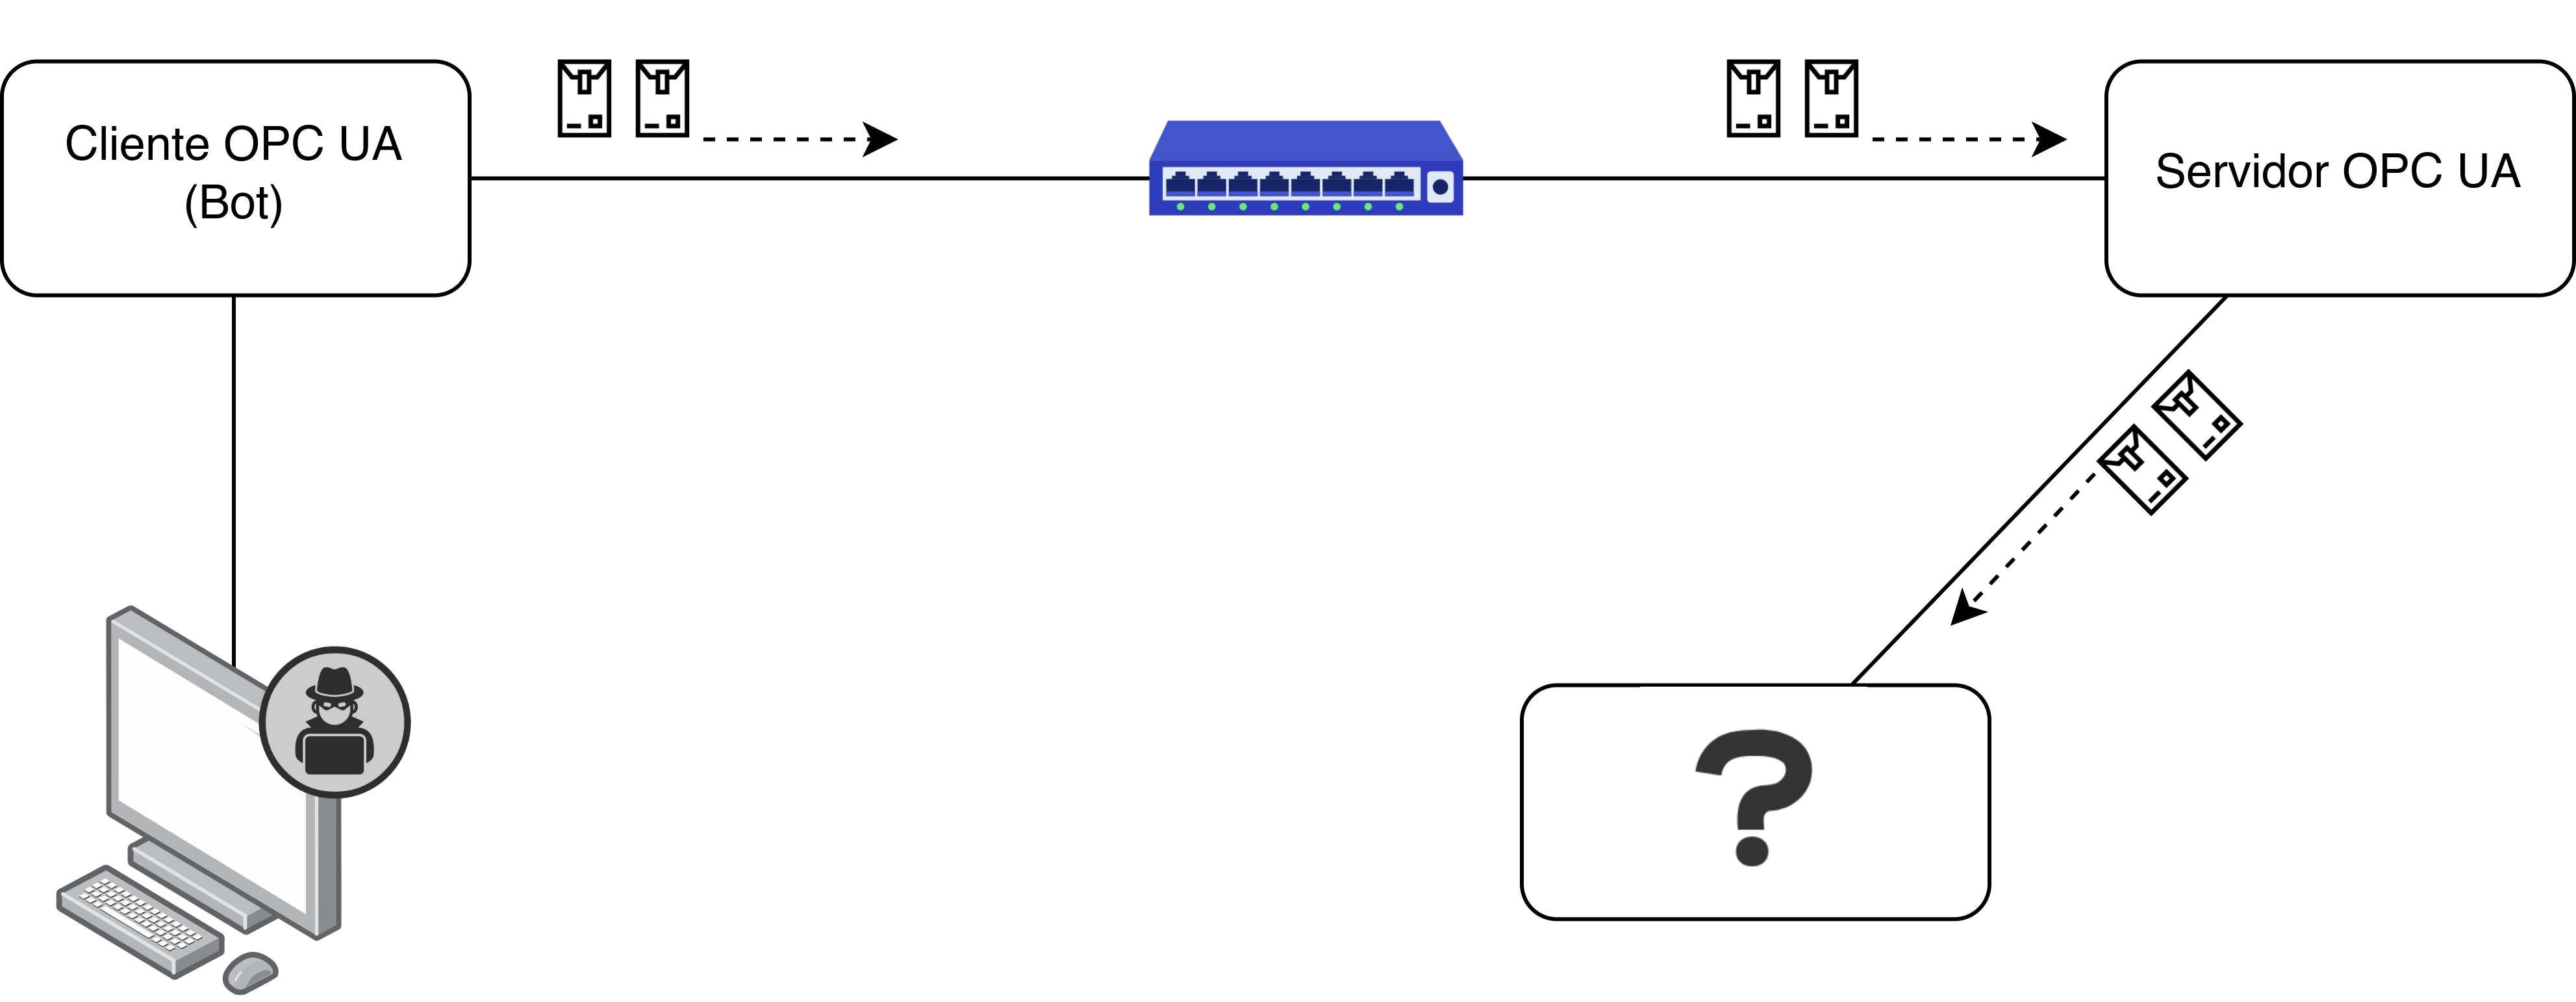
\includegraphics[width=0.9\textwidth]{USPSC-img/dos.png}
        \end{center}
        \legend{Fonte: elaborada pelo autor.}
    \end{figure}
    
    Existem diversos cenários possíveis para a efetuação do ataque de negação de serviço. Além do impacto da inundação na rede, ressaltam-se os efeitos no processamento do componente ao sofrer ataques intensivos, no qual o servidor precisa avaliar as certificações para responderem solicitações. Segundo \citeonline{neu2019}, os principais cenários são:

    \begin{enumerate}
        \item \underline{SYN \textit{Flooding}}: o cliente sobrecarrega o servidor enviando mensagens SYN de forma contínua, e o servidor responde com ACK a cada uma dessas mensagens. Embora essa ação possa inundar a rede com tráfego sobrecarregado com estas mensagens, seu impacto no consumo de recursos do servidor é limitado;
        \item \underline{ACK ou ERR \textit{Flooding}}: nesse cenário, o cliente inunda o servidor com mensagens ACK e/ou ERR, às quais o servidor responde com mensagens ERR. Da mesma forma do anterior, pode haver sobrecarga na rede, mas possui impacto moderado nos recursos do servidor;
        \item \underline{Inundação com Mensagens Incorretas}: são enviadas continuamente mensagens incorretas pelo Elemento Invasor, forçando respostas ERR pelo servidor. Também cria-se sobrecarga na rede, mas apresenta impacto relativamente baixo no processamento do servidor;
        \item \underline{CLO \textit{Flooding}}: enviam-se, repetidamente, mensagens de solicitação de fechamento de canal (CLO) ao servidor, que responde com mensagens ERR, sobrecarregando a rede com o tráfego destas mensagens.
        \item \underline{Inundação com \textbf{FindServers} ou \textbf{GetEndpoints}}: O cliente estabelece um canal no modo de segurança \textbf{None} e, em seguida, envia continuamente mensagens \textbf{FindServers()} ou \textbf{GetEndpoints()} para o servidor, que, por sua vez, responde com as mesmas mensagens por meio do OPC UA MSG. Apesar de apresentar impacto na rede, não altera os recursos do servidor;
        \item \underline{Inundação com Solicitações SYN e OPN}: um cliente não confiável realiza um ataque de negação de serviço enviando continuamente solicitações SYN e OPN ao servidor. O servidor responde com mensagens ACK e ERR. Nesse ataque, o servidor consome recursos substanciais durante a validação do certificado, na solicitação e no processo de criptografia da mensagem. Esse ataque pode ser ainda mais eficaz quando a Autoridade de Certificação está localizada em um sistema diferente, aumentando consideravelmente o tempo de validação do certificado, e, consequentemente, o processamento do componente onde se encontra o servidor.
    \end{enumerate}

    Duas ferramentas são utilizadas para efetuar a inundação da rede e, assim, alcançar o DoS: OPC UA Exploit Framework e Hping3, além de aplicar o Nmap para efetuar uma varredura da rede a fim de encontrar portas abertas e endereços IP disponíveis. 

    Uma vez que o Elemento Invasor obteve acesso a algum dos componentes da rede do alvo, o Nmap é utilizado para mapeamento da rede em questão. O comando abaixo executa um \textit{scan} SYN em um range de IPs, relativamente não-obstrusivo e camuflado, uma vez que ele nunca completa uma conexão TCP. Também chamado de escaneamento de portas entreabertas (\textit{half-open scanning}), um pacote SYN é enviado como se fosse abrir uma conexão real, cuja espera-se uma resposta. Um SYN/ACK indica que a porta está ouvindo (aberta), enquanto um RST (\textit{reset}) é indicativo de uma não-ouvinte. Se nenhuma resposta é recebida após diversas retransmissões, a porta é marcada como filtrada. A porta também é marcada como filtrada se um erro ICMP de inalcançável é recebido.

    \begin{minted}[
        breaklines,
        %linenos,
        mathescape,
        encoding=utf8,
        framesep=2mm,
        baselinestretch=1.2,
        bgcolor=codeback,
        fontsize=\footnotesize
    ]{console}
nmap -sS 192.168.164.*
    \end{minted}

    A correta execução desse mapeamento resulta em uma lista de IPs disponíveis e portas abertas, que servirão de entrada para os próximos passos. O Hping3 é utilizado para realizar o SYN \textit{Flooding} (1) na rede. Para isso, o \textit{script} de configuração abaixo deve ser implementado pelo Elemento Invasor, customizando-o de acordo com cada cenário.

    \begin{minted}[
        breaklines,
        %linenos,
        mathescape,
        encoding=utf8,
        framesep=2mm,
        baselinestretch=1.2,
        bgcolor=codeback,
        fontsize=\footnotesize
    ]{bash}
# CONFIGURAÇÃO
set TARGET "192.168.164.101"  # O alvo do ataque
set FAKEIP "192.168.164.201"  # Endereço falso
set BROADCAST "192.168.164.254"  # Endereço de broadcast da rede

set PORTS {{4840}{4192}}  # Utilizar as portas abertas encontradas no Nmap
set PORTUDP 123  # Utilizar uma porta UDP ativa

set commandRunTime 60

# EXECUÇÃO
foreach port $PORTS {
    lappend commands "hping3 -S -a $FAKEIP -p $port --flood -V $TARGET"
}
    \end{minted}

    Com isso, o Hping3 está preparado para iniciar o ataque direcionado ao endereço e portas especificados, com uma frequência predefinida (neste caso, sessenta segundos). A interpretação dos parâmetros utilizados na execução é a seguinte: o argumento \textbf{-S} define o tipo de ataque, \textbf{-p} identifica a porta de destino, \textbf{-V} indica o endereço IP do alvo, enquanto \textbf{-a} determina o endereço IP falsificado utilizado no ataque, uma estratégia que pode contornar \textit{firewalls} de forma eficaz.

    Por fim, alguns ataques mais robustos são efetuados com o auxílio da ferramenta OPC UA Exploit Framework. Os ataques de negação de serviço disponibilizados pelo \textit{framework} e escolhidos para execução no ambiente de simulação industrial proposto, são apresentados abaixo, seguidos de suas respectivas categorias, conforme os cenários supracitados e apresentados por \citeonline{neu2019}, e suas descrições:

    \begin{itemize}
        \item[N/A] \underline{Loop infinito na cadeia de certificados}: refere-se a uma situação em que algum servidor implementa a verificação da cadeia de certificados por conta própria, sem proteção contra um loop de cadeia infinita. Isso pode ocorrer quando um certificado A, por exemplo, é assinado por outro certificado B, que por sua vez é assinado pelo A. Cria-se uma dependência circular entre os certificados A e B, resultando em um loop infinito durante o processo de verificação da cadeia de certificados;
        % \item[(3)] \underline{Inundação por \textit{Chunk}}: envolve o envio de uma quantidade abundante de fragmentos de dados ao servidor sem o envio do fragmento final correspondente. O OPC UA permite a divisão dos dados em fragmentos, comumente chamados como \textit{MessageChunks} ou \textit{Chunks}, que são enviados à medida que são codificados, a fim de facilitar a transmissão e o processamento. Caso ocorra um erro na criação de um destes fragmentos, um \textit{Chunk} final deve ser enviado ao destinatário para notificar o erro, que por sua vez, é marcado com um sinalizador `A' (abortar) para indicar o erro. O receptor deve verificar a segurança do \textit{MessageChunk} abortado antes de processá-lo e, caso esteja tudo certo, ignorar a mensagem, mas sem encerrar o \textbf{SecureChannel};
        \item[(3)] \underline{Chamada da função \textit{Dereference} nula}: envolve a chamada de vários métodos OPC UA e encerramento da sessão antes da conclusão destes. Isso resulta em uma situação em que a aplicação servidora é forçada a referenciar um objeto nulo ou um ponteiro invalido, levando a um erro de execução;
        \item[(6)] \underline{Abertura de múltiplos canais seguros}: tentativa de inundação do servidor com uma quantidade abundante de solicitações \textbf{OpenSecureChannels};
        % \item[(3)] \underline{Mensagem aninhada complexa}: aplicação de uma variante especialmente manipulada e complexa, projetada para explorar vulnerabilidades em um servidor OPC UA. Quando esta variante é processada pelo servidor, ela pode causar um estouro na pilha de chamadas (\textit{call stack overflow}), levando a uma falha no servidor;
        \item[(5)] \underline{Tradução do caminho de navegação}: são enviadas ao servidor requisições de traduções de \textit{browse path} complexas que exploram a falta de limites adequados na resolução destes caminhos, podendo causar também um \textit{call stack overflow};
        % \item[Não aplicável] \underline{Falha de espera no \textit{Thread Pool}}: caracteriza uma paralisação (\textit{deadlock}) no sistema de \textit{Thread Pool} -- mecanismo de gerenciamento de \textit{threads} utilizado para processar solicitações de clientes e tarefas no servidor OPC UA -- devido à inanição simultânea de tarefas concorrentes. Em termos mais simples, quando vários processos ou \textit{threads} estão competindo por recursos do \textit{Thread Pools} de um servidor e, devido a problemas de sincronização ou gerenciamento inadequado de \textit{threads}, ficam em um estado de espera prolongado, impedindo efetivamente o servidor de processar solicitações legítimas;
        % \item[(6)] \underline{Persistência ilimitada de subscrições}: inúmeras solicitações de monitoramento ao servidor são enviados por um invasor, todas configuradas para não excluir os itens após o monitoramento. Esta persistência resulta em uma alocação descontrolada de recursos de memória pelo servidor, levando eventualmente a uma negação de serviço devido ao esgotamento de recursos.
        % \item[(3)] \underline{Chamada da função \textit{Dereference} nula}: envolve a chamada de vários métodos OPC UA e encerramento da sessão antes da conclusão destes. Isso resulta em uma situação em que a aplicação servidora é forçada a referenciar um objeto nulo ou um ponteiro invalido, levando a um erro de execução;
        % \item[(3)] \underline{Alteração de corrida e navegação no espaçamento de endereço}: o Elemento Invasor realiza a adição de \textit{Nodes} no \textit{Address Space} no servidor e, simultaneamente, remove-os em um ciclo contínuo, enquanto percorre todo o espaçamento de endereço. Esta manobra cria uma situação de competição na qual o servidor está sendo constantemente modificado e examinado ao mesmo tempo, podendo, assim, esgotar os recursos de processamento e resultar em problemas de consistência no \textit{Address Space};
        % \item[(6)] \underline{Atualização de condição ilimitada}: refere-se ao envio repetido e quantidade abundante de chamadas do método \textbf{ConditionRefresh}, o que leva a alocações de memória não controladas e, eventualmente, pode resultar em uma falha no sistema. O método ConditionRefresh é usado para atualizar as condições e estados das variáveis monitoradas em um servidor OPC UA.
    \end{itemize}

    Sabendo disso, os ataques acima podem ser efetuados através da seguinte linha de comando base, substituindo SERVER\_TYPE pelo tipo de servidor utilizado (\textit{e.g.}, softing, unified, prosys, kepware, triangle, dotnetstd, open62541, ignition, rust, node-opcua, opcua-python, milo e s2opc), IP\_ADDR pelo endereço de IP do alvo, PORT pela porta aberta para a comunicação UA, ENDPOINT\_ADDRESS pelo endpoint do servidor, FUNC\_TYPE pelo tipo de ataque escolhido (verificar na documentação oficial do framework quais os nomes das funções disponíveis \cite{claroty2023}) e DIR, necessário para algumas funções:

    \begin{minted}[
        breaklines,
        %linenos,
        mathescape,
        encoding=utf8,
        framesep=2mm,
        baselinestretch=1.2,
        bgcolor=codeback,
        fontsize=\footnotesize
    ]{console}
python main.py [SERVER_TYPE] [IP_ADDR] [PORT] [ENDPOINT_ADDRESS] [FUNC_TYPE] [DIR*]
    \end{minted}

\section{Metodologia}

    O fluxograma apresentado na \autoref{fig:flux} explicita a sequência e estrutura de atividades, os passos que compõem a metodologia, posteriormente explicados nas subseções.
    
    \begin{figure}[htbp!]
        \caption{\label{fig:flux}Fluxograma da metodologia proposta}
        \begin{center}
            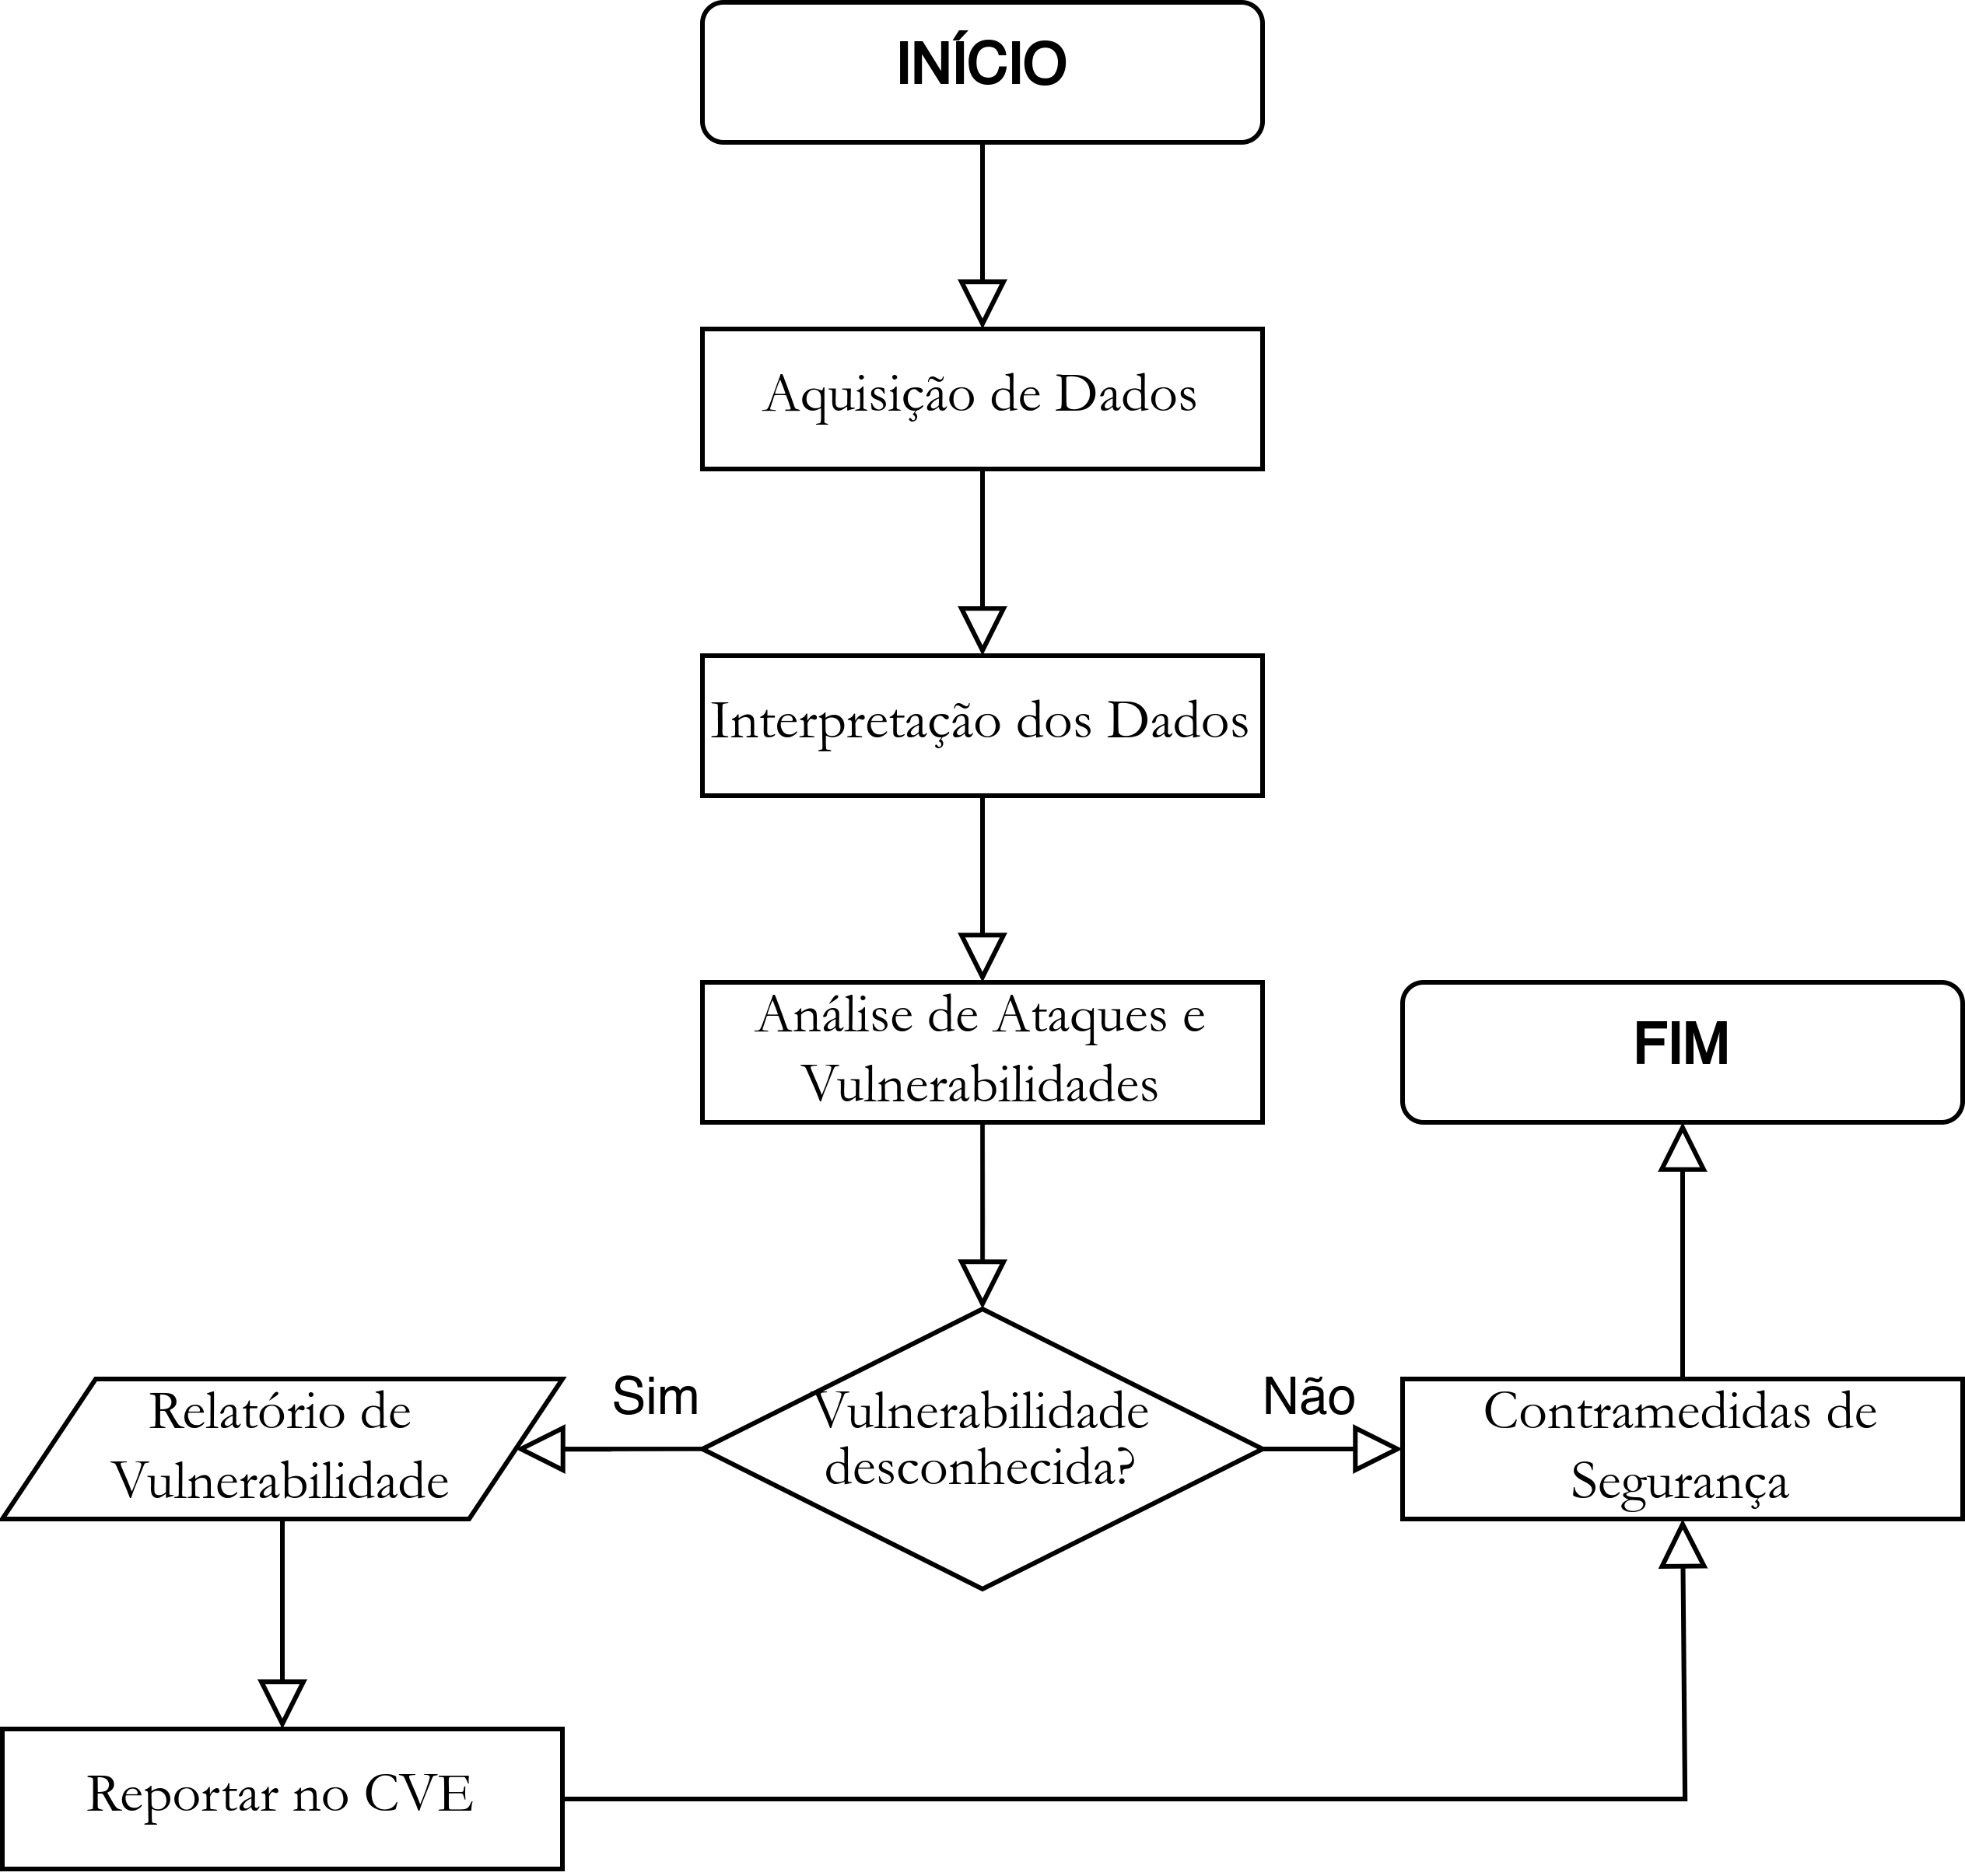
\includegraphics[width=0.7\textwidth]{USPSC-img/fluxograma.png}
        \end{center}
        \legend{Fonte: elaborada pelo autor.}
    \end{figure}

    Para a realização adequada do experimento proposto neste estudo, a infraestrutura de rede do protocolo OPC UA foi configurada conforme os seguintes parâmetros: o Raspberry Pi atuando como servidor e a DF63 NG desempenhando o papel de cliente. Além disso, um elemento de rede chamado `Sniffer' (conforme ilustrado na \autoref{fig:banc}) foi inserido na configuração para monitorar e registrar a comunicação da rede. Com o propósito de fornecer uma visão clara dos componentes envolvidos e facilitar a análise dos dados coletados durante o experimento, os endereços IP e MAC de cada elemento do sistema estão resumidos na \autoref{tab:ender}. Importante mencionar que o servidor OPC UA foram configurados para utilizar a porta padrão 4840, e os \textit{endpoints} correspondentes adotam o padrão abaixo. Essa estrutura de configuração foi essencial para a condução eficaz do experimento e a subsequente análise dos resultados.

    \begin{minted}[
        breaklines,
        %linenos,
        mathescape,
        encoding=utf8,
        framesep=2mm,
        baselinestretch=1.2,
        bgcolor=codeback,
        fontsize=\footnotesize
    ]{console}
<esquema>://<endereço>:<porta>/<DiscoveryEndpoint>
    \end{minted}

    Onde, `<esquema>' pode ser `opc.tcp' ou `opc.https', `<endereço>' é o endereço IP do servidor, `<porta>' é a porta de comunicação OPC UA, e `<DiscoveryEndpoint>' é o ponto de descoberta do servidor OPC UA.

    \begin{table}[htbp!]
        \centering
        \caption{Endereços IP e MAC dos equipamentos da rede OPC UA}%
        \label{tab:ender}
        \begin{tabular}{ccc}
            \toprule
            \thead{Equipamento} & \thead{IP} & \thead{MAC} \\
            \toprule
            DF63 NG  & 192.168.164.101 & 00:30:5C:24:13:66 \\
            \midrule
            RaspPi   & 192.168.164.102 & E4:5F:01:2E:1A:B6 \\
            % \midrule
            % RaspPi 2 & 192.168.164.102 & E4:5F:01:2E:1B:C1 \\
            \midrule
            Sniffer  & 192.168.164.201 & C8:3A:35:49:FD:58 \\
            \midrule
            Invasor  & 192.168.164.115 & 00:be:43:34:b8:54/00:09:5B:a0:5F:F0 \\
            \bottomrule
        \end{tabular}
        \fonte{elaborada pelo autor.}%
    \end{table}

    \subsection{Aquisição de Dados} \label{sec:aquisicao}

    A fase de aquisição de dados fundamenta-se na captura do tráfego de pacotes transmitidos pela rede OPC UA durante a comunicação entre a aplicação servidora e o cliente da rede, enquanto ocorrem os ataques. Esse processo se baseia na utilização do software Wireshark, no qual permite a coleta de informações cruciais sobre a comunicação, incluindo detalhes como o tipo de protocolo empregado, a origem e o destino dos dados. As informações capturadas são armazenadas em ordem cronológica com a capacidade de serem salvas em arquivos no formato `.pcapng'. O software Wireshark foi configurado para finalizar a captura com sessenta segundos de coleta.

    Os alvos dos ataques é o servidor OPC UA, e em cada cenário, o elemento \textit{Sniffer} é configurado para realizar a captura do tráfego gerado por estes ataques. Para organizar os pacotes capturados, foi adotada a seguinte nomenclatura de arquivos: `[Modo de Segurança]-[Tipo do Ataque]-[Número da Captura].pcapng'. Aqui, o modo de segurança pode assumir os valores 0 (None), 1 (Sign) e 2 (Sign\&Encrypt). Os tipos de ataques correspondem àqueles detalhados na \autoref{sec:attacks} (`sniffing', `mitm' e `dos-[função]'), e o número da captura é representado por um dígito de 0 a 9. Por exemplo, para salvar a terceira captura obtida durante uma negação de serviço pelo ataque de chamada da função \textit{Dereference} nula, com a rede configurada no modo de segurança \textbf{Sign}, o arquivo seria nomeado como: `1-dos\_function\_call\_null\_deref.pcapng'. A \autoref{tab:attacks} apresenta os cenários e os arquivos de captura gerados durante os experimentos para cada tipo de ataque.

    \begin{table}[htbp]
        \centering
        \caption{Arquivos de captura gerados para cada cenário durante a fase de aquisição de dados}%
	    \label{tab:attacks}
        \begin{tabular}{B{1.5cm}B{3cm}B{5.5cm}B{3.5cm}}
        \toprule
            Cenário & Modo de Segurança & Arquivo (.pcapng) & Descrição do Ataque \\
        \end{tabular}
        \begin{tabular}{M{1.5cm}N{3cm}N{5.5cm}N{3.5cm}}
            \toprule
            C1 & None & \code{0-dos\_certificate\_inf\_chain\_loop} & \multirow{3}{*}{\parbox{3.5cm}{DoS pelo loop infinito na cadeia de certificados}} \\
            C2 & Sign & \code{1-dos\_certificate\_inf\_chain\_loop} & \\
            C3 & Sign \& Encrypt & \code{2-dos\_certificate\_inf\_chain\_loop} & \\
            \midrule
            C4 & None & \code{0-dos\_function\_call\_null\_deref} & \multirow{3}{*}{\parbox{3.5cm}{DoS pela chamada da função \textit{Dereference} nula}} \\
            C5 & Sign & \code{1-dos\_function\_call\_null\_deref} & \\
            C6 & Sign \& Encrypt & \code{2-dos\_function\_call\_null\_deref} & \\
            \midrule
            C7 & None & \code{0-dos\_hping3} & \multirow{3}{*}{\parbox{3.5cm}{DoS pela inundação do TCP/IP}} \\
            C8 & Sign & \code{1-dos\_hping3} & \\
            C9 & Sign \& Encrypt & \code{2-dos\_hping3} & \\
            \midrule
            C10 & None & \code{0-dos\_open\_multiple\_channels} & \multirow{3}{*}{\parbox{3.5cm}{DoS pela abertura de múltiplos canais seguros}} \\
            C11 & Sign & \code{1-dos\_open\_multiple\_channels} & \\
            C12 & Sign \& Encrypt & \code{2-dos\_open\_multiple\_channels} & \\
            \midrule 
            C13 & None & \code{0-dos\_translate\_browse\_path\_call} & \multirow{3}{*}{\parbox{3.5cm}{DoS pela tradução do caminho de navegação}} \\
            C14 & Sign & \code{1-dos\_translate\_browse\_path\_call} & \\
            C15 & Sign \& Encrypt & \code{2-dos\_translate\_browse\_path\_call} & \\
            \midrule
            C16 & None & \code{0-mitm\_arp} & \multirow{3}{*}{\parbox{3.5cm}{MITM pela falsificação da tabela ARP}} \\
            C17 & Sign & \code{1-mitm\_arp} & \\
            C18 & Sign \& Encrypt & \code{2-mitm\_arp} & \\
            \midrule
            C19 & None & \code{0-mitm\_port} & \multirow{3}{*}{\parbox{3.5cm}{MITM pelo roubo de portas}} \\
            C20 & Sign & \code{1-mitm\_port} & \\
            C21 & Sign \& Encrypt & \code{2-mitm\_port} & \\
            \midrule
            C22 & None & \code{0-sniffing} & \multirow{3}{*}{\parbox{3.5cm}{\textit{Packet Sniffing}}} \\
            C23 & Sign & \code{1-sniffing} & \\
            C24 & Sign \& Encrypt & \code{2-sniffing} & \\
            \midrule
            C25 & None & \code{0-normal\_local\_server} & \multirow{3}{*}{\parbox{3.5cm}{Comunicação normal entre cliente e servidor}} \\
            C26 & Sign & \code{1-normal\_local\_server} & \\
            C27 & Sign \& Encrypt & \code{2-normal\_local\_server} & \\
            \bottomrule
        \end{tabular}
        \fonte{elaborada pelo autor.}%
    \end{table}

    Além disso, é importante salientar que durante o processo de coleta de dados com o Wireshark, simultaneamente, obtêm-se informações sobre a carga de processamento da CPU nos hospedeiros do servidor OPC UA. Essa abordagem complementa significativamente a análise dos efeitos do ataque sobre o desempenho do sistema. Para viabilizar esse monitoramento, desenvolveu-se um \textit{script} que deve ser ativado pelo elemento \textit{Sniffer} no início da captura de dados.

    \begin{minted}[
        breaklines,
        %linenos,
        mathescape,
        encoding=utf8,
        framesep=2mm,
        baselinestretch=1.2,
        bgcolor=codeback,
        fontsize=\footnotesize
    ]{python}
import csv
import time
import os

def get_cpu_usage():
    """
    Calcula a utilização da CPU em percentual.
    """
    with open('/proc/stat') as stat_file:
        lines = stat_file.readlines()
    # Obtém os valores de CPU da primeira linha
    cpu_values = [int(val) for val in lines[0].split()[1:8]]
    # Soma os valores da CPU para obter o total de utilização da CPU
    total_cpu_time = sum(cpu_values)
    # Calcula a diferença entre a utilização da CPU atual e anterior
    delta_total_cpu_time = total_cpu_time - get_cpu_usage.previous_total_cpu_time
    delta_idle_cpu_time = cpu_values[3] - get_cpu_usage.previous_idle_cpu_time  # 4º valor é o tempo ocioso
    # Calcula a taxa de utilização da CPU em percentual
    cpu_percent = 100 * (1 - delta_idle_cpu_time / delta_total_cpu_time)
    # Atualiza os valores anteriores para a próxima iteração
    get_cpu_usage.previous_total_cpu_time = total_cpu_time
    get_cpu_usage.previous_idle_cpu_time = cpu_values[3]

    return cpu_percent

# Inicializa os valores anteriores
get_cpu_usage.previous_total_cpu_time = 0
get_cpu_usage.previous_idle_cpu_time = 0

def get_memory_usage():
    """
    Calcula a utilização da memória em percentual.
    """
    total_memory = float(os.popen("grep 'MemTotal' /proc/meminfo | awk '{print $2}'").read().strip())
    available_memory = float(os.popen("grep 'MemAvailable' /proc/meminfo | awk '{print $2}'").read().strip())
    used_memory = total_memory - available_memory
    memory_percent = (used_memory / total_memory) * 100
    return memory_percent

def main():
    """
    Função principal que realiza a coleta de dados de utilização da CPU e memória, e salva em um arquivo CSV.
    """
    output_file = '1-dos_hping3.csv'
    duration = 60  # Tempo de execução em segundos

    # Abre o arquivo CSV para escrita
    with open(output_file, mode='w', newline='') as file:
        writer = csv.writer(file)
        writer.writerow(['Timestamp', 'CPU (%)', 'Memory (%)'])

        start_time = time.time()

        while time.time() - start_time <= duration:
            timestamp = time.time() - start_time
            timestamp_str = '{:.6f}'.format(timestamp)
            cpu_usage = round(get_cpu_usage(), 2)
            memory_usage = round(get_memory_usage(), 2)

            writer.writerow([timestamp_str, cpu_usage, memory_usage])
            time.sleep(1)  # Captura de dados a cada segundo

if __name__ == "__main__":
    main()
    \end{minted}

    A implementação desta aquisição visa fornecer uma visão integrada do impacto dos ataques não apenas em termos de tráfego de rede, mas também em termos de uso de recursos do sistema, permitindo uma análise mais abrangente das vulnerabilidades e seus efeitos nas operações dos sistemas OPC UA. Esse monitoramento contínuo possibilita a identificação de padrões de comportamento anômalo que podem ser associados a atividades maliciosas, além de fornecer dados quantitativos que auxiliam na avaliação do impacto real dos ataques.

    Para garantir a precisão e a confiabilidade dos dados coletados, cada ataque foi repetido múltiplas vezes, e as capturas resultantes foram analisadas de forma comparativa. Esse método permite a identificação de variações nos resultados que possam ser atribuídas a fatores externos ou a inconsistências na execução dos ataques. Todas as capturas foram realizadas em um ambiente controlado, com a configuração dos dispositivos de rede e do servidor OPC UA mantida constante ao longo dos experimentos.

    \subsection{Interpretação dos Dados}

    Uma vez que o tráfego da rede é coletado para cada ataque e salvos nos arquivos de captura, os dados podem ser interpretados para o estudo de vulnerabilidades nos cenários propostos.  A análise detalhada dos dados capturados durante os ataques cibernéticos em redes OPC UA é fundamental para entender o impacto das vulnerabilidades exploradas. Assim, uma nova aplicação denominada \textbf{uanalyser} foi desenvolvida para auxiliar na interpretação dos dados capturados, permitindo a geração de gráficos específicos para cada cenário de ataque. A seguir, apresenta-se como os dados obtidos foram interpretados, destacando a importância dos gráficos gerados e a relevância da análise dos atributos monitorados.

    A geração dos gráficos visa fornecer uma representação visual dos principais indicadores de desempenho e segurança da rede OPC UA sob ataque. Logo, quatro gráficos são gerados para cada coleta: (a) \textit{Throughput} (kbps), (b) desempenho do hospedeiro do servidor OPC UA (RAM e CPU), (c) quantidade de pacotes OPC UA por segundo e (d) \textit{Round Trip Time} (RTT) normalizado, por pacote. Esses gráficos foram escolhidos devido à sua capacidade de ilustrar diferentes aspectos do funcionamento e da resiliência ou fragilidade da rede em condições adversas.

    Para a construção do \textbf{uanalyser}, utilizou-se a linguagem de programação Python e os seguintes pacotes essenciais para a obtenção dos resultados em gráficos: Scapy, Matplotlib, NumPy e Pandas, além de contar com os pacotes para o ambiente de desenvolvimento: MkDocs, PyTest e Taskipy.

    O Scapy é uma ferramenta poderosa para manipulação de pacotes de rede, que facilita a captura, a análise e a criação de pacotes, independentemente de pilhas predefinidas ou regras de rede comuns. Logo, utilizando os recursos desse pacote, o \textbf{uanalyser} lê arquivos de captura no formato .pcapng, extrai informações específicas dos pacotes e realiza análises detalhadas. O diagrama de sequência da aplicação é apresentado na \autoref{fig:seqUanalyser} e detalha como é realizada a interpretação destes dados. São construídos alguns gráficos que mostram como cada ataque afeta a rede em termos de \textit{throughput}, uso de recursos do hospedeiro, quantidade de pacotes por segundo e RTT.

    \begin{figure}[htbp!]
        \caption{\label{fig:seqUanalyser}Diagrama de sequência da aplicação \textbf{uanalyser}}
        \begin{center}
            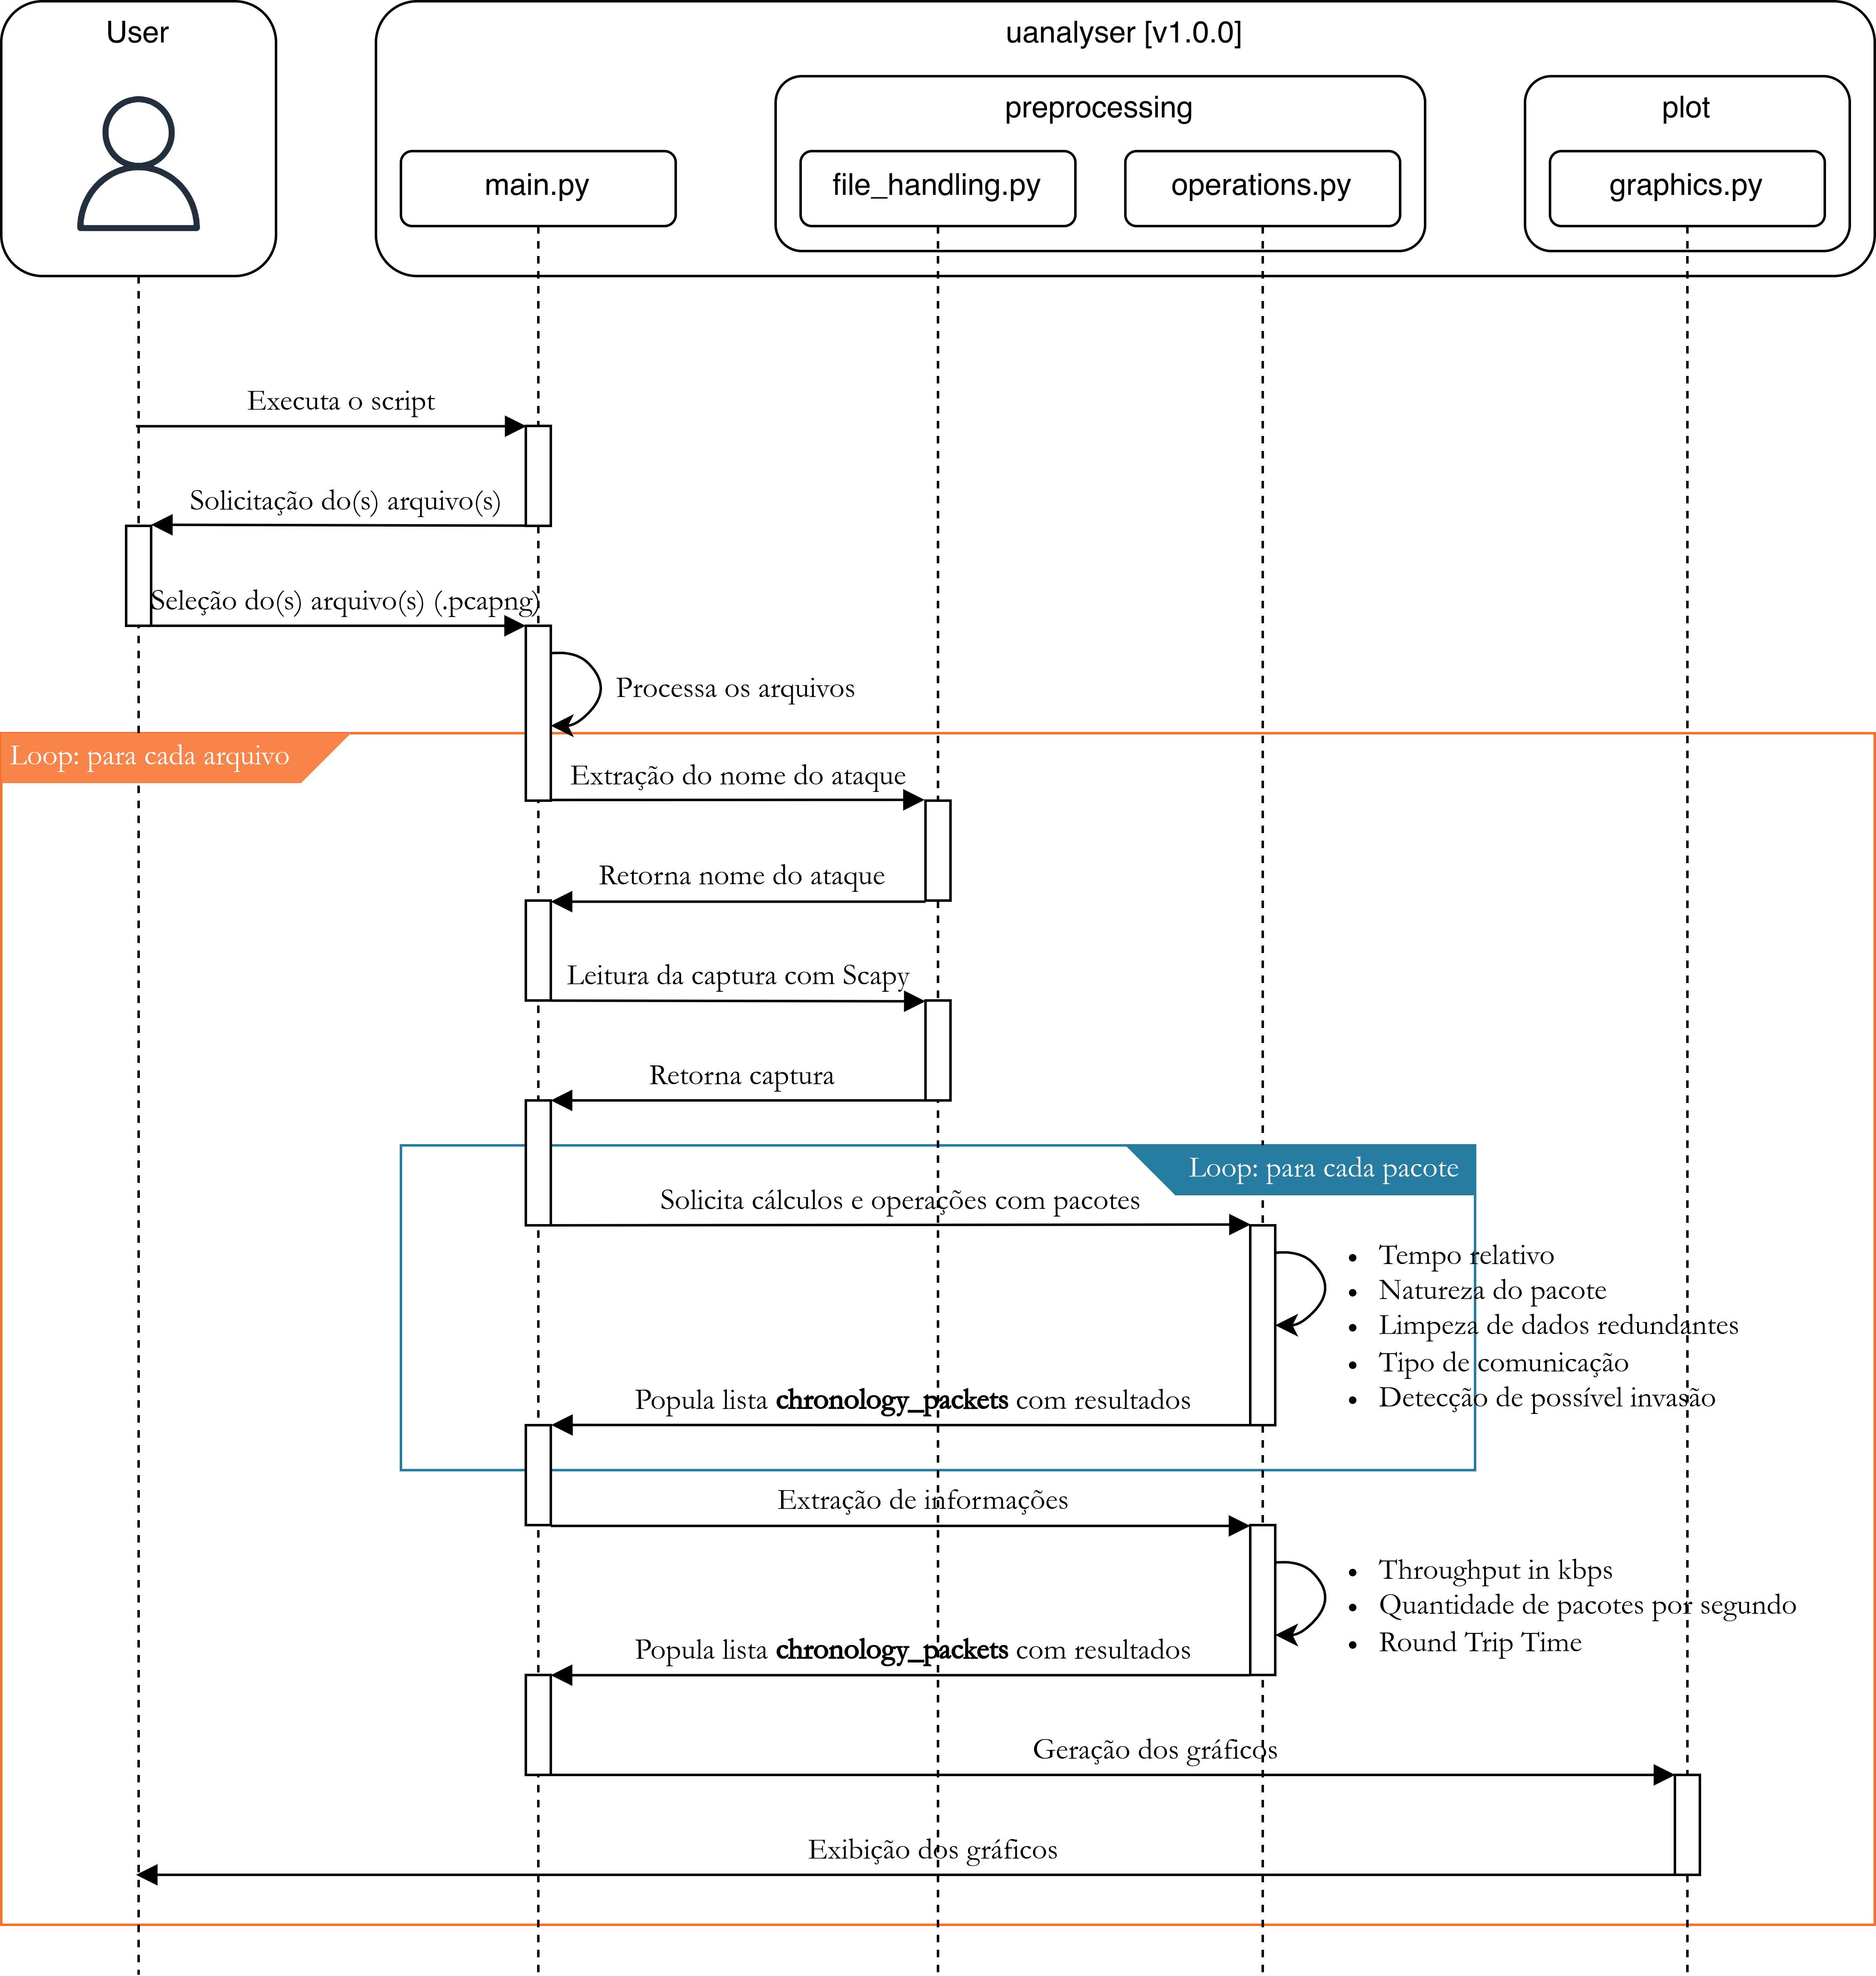
\includegraphics[width=0.972\textwidth]{USPSC-img/seqUanalyser.png}
        \end{center}
        \legend{Fonte: elaborada pelo autor.}
    \end{figure}

    Dentro do contexto do protocolo OPC UA, as mensagens trocadas entre cliente e servidor podem incluir várias estruturas de dados, como mensagens de sessão, mensagens de serviço e dados de publicação/subscrição. Cada tipo de mensagem tem seu próprio formato e estrutura, conforme especificado pelo padrão OPC UA. A análise dessas mensagens é crucial para identificar comportamentos anômalos e potenciais vulnerabilidades.

    A análise dos pacotes capturados e a visualização dos gráficos gerados pelo \textbf{uanalyser} permitem uma compreensão detalhada dos efeitos dos ataques nas redes OPC UA. Essa abordagem sistemática e visual facilita a identificação de vulnerabilidades específicas do protocolo e o desenvolvimento de contramedidas eficazes para melhorar a segurança e a resiliência das redes industriais.

    O software desenvolvido para este trabalho está disponível no GitHub \footnote{Disponível em: \url{https://github.com/JonathanTSilva/opcua-analyser}. Acesso em: 04 jul. 2024} e aberto para contribuições. Aqueles que desejarem contribuir devem seguir os padrões de desenvolvimento estabelecidos no arquivo \texttt{contributing.md} e aderir ao código de conduta do projeto.

    \subsection{Análise dos Ataques e Vulnerabilidades}

    A análise de ataques e vulnerabilidades em redes industriais OPC UA é um processo sistemático e detalhado que visa identificar, avaliar e mitigar possíveis pontos fracos no protocolo e na implementação de redes OPC UA. Esta etapa é essencial para garantir a segurança e a continuidade operacional dos IACSs e consiste na análise dos resultados da série de testes e simulações de ataques cibernéticos obtidos nos processos anteriores. Cada tipo de ataque explora diferentes vulnerabilidades potenciais do protocolo e da infraestrutura de rede.

    Ao testar vulnerabilidades da comunicação em redes industriais OPC UA, foca-se na determinação da qualidade da comunicação durante e após um ataque. Em outras palavras, se o equipamento é capaz de desempenhar sua tarefa nestes períodos. Adicionalmente, é examinado se o alvo sofre com falta de resposta ou respostas incomuns.

    Como a observação de soluções existentes faz parte da abordagem deste desenvolvimento, precisamos ter algum ponto de referência como base para nossas observações das vulnerabilidades existentes e comportamento durante ataques. Com base nisso, são definidas as seguinte classes de vulnerabilidades para este projeto em específico:

    \begin{itemize}
        \item \textbf{Classe 1}: falhas que interrompem o comunicação OPC UA entre os agentes, afetando a disponibilidade;
        \item \textbf{Classe 2}: serviços interrompidos ou comportamento inesperado que não alteram a comunicação, mas prejudica a integridade;
        \item \textbf{Classe 3}: vulnerabilidades que não interrompem a comunicação, mas afetam a confiabilidade.
    \end{itemize}

    A partir dos gráficos gerados e do comportamento da rede e dispositivos durante e após o ataque, é possível identificar as vulnerabilidades existentes e classificá-las de acordo com as classes supracitadas. Além disso, é possível verificar a eficácia das diferentes políticas de segurança do OPC UA (`None', `Sign', `Sign \& Encrypt'). A análise dos resultados obtidos é essencial para a identificação de possíveis falhas e a proposição de medidas corretivas e preventivas para mitigar os riscos de segurança nas redes OPC UA.

    Essa abordagem metodológica, que inclui a observação de gráficos de throughput, desempenho de RAM e CPU, quantidade de pacotes OPC UA por segundo e RTT normalizado, permite uma compreensão detalhada do impacto dos ataques nas redes industriais OPC UA. Com isso, é possível desenvolver estratégias de mitigação eficazes e assegurar a robustez e a resiliência das redes contra possíveis ameaças cibernéticas.
    
    \subsection{Relatório de Vulnerabilidade}

    A construção de um relatório de vulnerabilidade é uma etapa crucial no processo de avaliação de segurança cibernética, especialmente no contexto de redes industriais OPC UA. Através deste relatório, é possível documentar e comunicar as vulnerabilidades identificadas, fornecer uma análise detalhada dos riscos e propor contramedidas adequadas. Este documento é fundamental não apenas para entender as falhas de segurança, mas também para tomar ações corretivas eficazes e melhorar a postura de segurança da organização.

    A elaboração de um relatório de vulnerabilidade deve seguir padrões internacionais de segurança cibernética e estar alinhada com as melhores práticas do setor. Um bom relatório deve ser estruturado de forma clara e objetiva, contemplando diferentes níveis de detalhamento para atender a diversos públicos, desde executivos até equipes técnicas.

    O relatório de vulnerabilidade é essencial para diversos stakeholders dentro de uma organização. Ele auxilia os executivos a compreenderem a postura de segurança atual da empresa e a justificarem investimentos em segurança. Para a equipe de TI, o relatório oferece detalhes técnicos sobre as vulnerabilidades descobertas e orientações sobre como corrigi-las. Além disso, o relatório pode ser utilizado para fins de conformidade regulatória, sendo compartilhado com auditores e reguladores para demonstrar os esforços de segurança da organização.

    Para garantir a eficácia do relatório de vulnerabilidade, ele deve incluir as seguintes seções principais:

    \begin{itemize}
        \item \underline{Sumário Executivo}: Uma visão geral de alto nível da avaliação, destinada a executivos não técnicos. Esta seção deve ajudar os executivos a avaliarem a postura de segurança da empresa e destacar quaisquer questões críticas que possam impactar a segurança corporativa ou a conformidade regulatória.
        \item \underline{Visão Geral}: Uma seção voltada para um público mais técnico, fornecendo um resumo da avaliação. Deve incluir informações sobre os sistemas analisados, ferramentas utilizadas e o número e a severidade das vulnerabilidades descobertas.
        \item \underline{Detalhes da Avaliação}: Esta seção deve fornecer detalhes técnicos sobre como a avaliação de vulnerabilidade foi conduzida. Deve descrever as etapas realizadas em cada fase da avaliação e seus resultados, permitindo que o leitor possa replicar os achados da avaliação.
        \item \underline{Resultados}: Esta seção deve detalhar os achados da avaliação. As vulnerabilidades devem ser classificadas por severidade para chamar a atenção para os maiores problemas dentro do ambiente da organização. Para cada vulnerabilidade potencial verificada, esta seção deve descrever o resultado, os sistemas afetados, o nível de severidade e fornecer um link para informações adicionais, como um CVE.
        \item \underline{Mitigações Recomendadas}: O objetivo de uma avaliação de vulnerabilidade é ajudar a organização a melhorar sua postura de segurança. Portanto, fornecer recomendações de mitigação é essencial. Em muitos casos, isso pode ser tão simples quanto recomendar uma atualização de software, uma senha mais forte em um sistema ou uma alteração em uma configuração de segurança insegura.
    \end{itemize}

    Uma vez que o relatório de vulnerabilidade é elaborado, ele deve ser aplicado nas bases de conhecimento da organização para garantir que todas as vulnerabilidades identificadas sejam tratadas de forma adequada. O relatório deve ser revisado regularmente e atualizado conforme novas vulnerabilidades sejam descobertas e medidas corretivas sejam implementadas. Além disso, é importante que o relatório siga os padrões globais de cibersegurança, como o CVE (do inglês \textit{Common Vulnerabilities and Exposures}) e os padrões de segurança IEC 62443, para garantir a consistência e a confiabilidade das informações.

    A utilização de frameworks reconhecidos internacionalmente, como o CVE e o IEC 62443, proporciona uma base sólida para a identificação e a classificação de vulnerabilidades. Estes padrões oferecem diretrizes claras sobre como avaliar e mitigar riscos, além de promover a adoção de práticas de segurança consistentes e eficazes. Além disso, existem diversos modelos para a elaboração de relatórios de vulnerabilidade, como o da CISA (Cybersecurity and Infrastructure Security Agency), do NIST (National Institute of Standards and Technology), que podem ser adaptados para atender às necessidades específicas de cada organização. Caso alguma vulnerabilidade desconhecida do protocolo OPC UA seja encontrada, será utilizado o modelo de relatório personalizado e disponibilizado no \autoref{ap:relatorio} para documentar e comunicar a descoberta.

    \subsection{Contramedidas de Segurança}

    Uma implementação bem projetada e sem complicações das contramedidas de segurança é uma das principais medidas para minimizar os riscos cibernéticos e maximizar a disponibilidade dos IACS. A segurança das redes industriais OPC UA deve contemplar uma abordagem holística, que inclua a proteção dos ativos de informação, a prevenção de ameaças e a detecção de incidentes.

    A determinação das contramedidas variam de acordo com o cenário de ataque e as vulnerabilidades identificadas. No entanto, algumas práticas comuns podem ser adotadas para fortalecer a segurança das redes OPC UA. Entre as principais contramedidas recomendadas estão:

    \begin{itemize}
        \item \underline{Criptografia e modos de seguranças:} conforme recomendado pelas políticas de segurança `Sign' e `Sign \& Encrypt', a criptografia e assinatura da comunicação OPC UA se destacam como as principais melhorias na configuração de segurança. Isso inclui a utilização de certificados robustos e algoritmos de criptografia atualizados.
        \item \underline{Alto nível de autenticação:} implementação de métodos de autenticação forte para acesso aos servidor OPC UA, incluindo autenticação multifator (MFA) e uso de certificados digitais para a autenticação de dispositivos.
        \item \underline{Apriomaramento da segurança da rede:} criação de zonas de segurança dentro da rede industrial para limitar a propagação de ataques, de acordo com o modelo de defesa em profundidade (do inglês \textit{defense in depth}), na qual cada zona é separada por \textit{firewalls} e dispositivos de segurança que monitoram e controlam o tráfego de rede. O modelo \textit{Zero Trust} se destaca atualmente como uma abordagem complementar à segregação de rede ao operar sob a premissa de "nunca confiar, sempre verificar". Considera-se que a rede é inerentemente insegura e que a confiança deve ser verificada continuamente, exigindo autenticação e autorização rigorosas para cada tentativa de acesso. 
        \item \underline{Controle de Acesso Baseado em Função (RBAC, do inglês \textit{Role-Based Access Control}):} aplicado para limitar o acesso aos recursos de rede e serviços da comunicação apenas aos usuários e dispositivos autorizados, minimizando o risco de acessos não autorizados.
        \item \underline{Monitoramento contínuo:} implementação de sistemas de monitoramento contínuo para detectar atividades anômalas e potenciais ataques em tempo real. Os IDS (do inglês \textit{Intrusion Detection Systems}) e SIEM (do inglês \textit{Security Information and Event Management}) se destacam como sistemas eficazes utilizados para garantir esse diagnóstico contínuo.
        \item \underline{Resposta a incidentes:} um bom plano de resposta a incidentes que define procedimentos claros para identificar, conter e remediar ataques cibernéticos é imprescindível para mitigar possíveis ataques às redes industriais. Este plano pode ser baseado nas melhores práticas recomendadas pela norma IEC 62443 e frameworks de segurança correlatos.
        \item \underline{Atualizações regulares:} garantia de que todos os componentes da rede, incluindo servidor OPC UA e dispositivos de rede, estejam sempre atualizados com os últimos \textit{patches} de segurança.
        \item \underline{\textit{Hardening} de sistemas:} aplicação de técnicas de \textit{hardening} para reduzir a superfície de ataque do servidor e dispositivos de rede. Isso inclui a desativação de serviços desnecessários, configuração segura de sistemas operacionais e aplicações, e implementação de políticas de segurança rígidas.
    \end{itemize}

    A determinação e implementação de contramedidas de segurança em redes industriais OPC UA é um processo complexo, mas essencial para garantir a segurança e a integridade dos sistemas de automação e controle. Através da combinação de análise detalhada de vulnerabilidades, referência a frameworks de segurança reconhecidos e avaliação contínua da eficácia das medidas implementadas, é possível desenvolver uma abordagem robusta para proteger redes OPC UA contra uma ampla gama de ameaças cibernéticas. Este trabalho contribui para o fortalecimento da segurança nas redes industriais, promovendo a resiliência dos sistemas críticos em um cenário de ameaças em constante evolução.

    % {\color{red}

    % Análise de Vulnerabilidades Conhecidas:

    % Utilizamos o banco de dados CVE para identificar vulnerabilidades conhecidas no protocolo OPC UA e em suas implementações. Cada CVE fornece detalhes sobre a vulnerabilidade, incluindo sua descrição, impacto e formas recomendadas de mitigação. Comparando essas vulnerabilidades com os resultados dos testes realizados, conseguimos correlacionar diretamente vulnerabilidades conhecidas com novas descobertas.

    % Referência a Padrões de Segurança:

    % Adotamos as diretrizes fornecidas pela norma IEC 62443, que é um conjunto de padrões desenvolvidos especificamente para a segurança de sistemas de automação e controle industrial. A IEC 62443 abrange desde os requisitos de segurança do produto até a gestão de segurança no ciclo de vida. Implementamos práticas recomendadas, como segmentação de rede, controle de acesso baseado em função e monitoramento contínuo de segurança.

    % Frameworks Adicionais:

    % Consultamos outros frameworks de segurança, como o NIST Cybersecurity Framework, para complementar nossas estratégias de mitigação com práticas amplamente aceitas e validadas. Integrando recomendações de múltiplos frameworks, criamos um conjunto robusto e abrangente de contramedidas.
    
    % A eficácia das contramedidas implementadas foi avaliada através de novos testes e simulações de ataques, utilizando o mesmo ambiente experimental. As principais atividades de avaliação incluíram:

    % Reexecução dos Ataques:

    % Realizamos novos testes de ataques cibernéticos sob as mesmas condições iniciais, mas com as contramedidas aplicadas. Isso permitiu a comparação direta dos resultados antes e depois da implementação das contramedidas. Monitoramos os indicadores de desempenho, como throughput, utilização de CPU e RAM, quantidade de pacotes por segundo e RTT, para verificar melhorias na resiliência da rede.

    % Análise Comparativa:

    % Comparamos os dados coletados durante os testes pós-contramedidas com os dados originais, para identificar reduções nos impactos dos ataques e melhorias na segurança da rede. Avaliamos a eficácia das contramedidas utilizando métricas de segurança, como a redução na taxa de sucesso dos ataques e o tempo de recuperação após incidentes.

    % Feedback e Melhoria Contínua:

    % Reavaliamos continuamente as contramedidas com base no feedback dos testes e na evolução das ameaças cibernéticas. Ajustes e melhorias foram implementados conforme necessário para garantir a proteção contínua da rede OPC UA.

    % Conclusão
    % A determinação e implementação de contramedidas de segurança em redes industriais OPC UA é um processo complexo, mas essencial para garantir a segurança e a integridade dos sistemas de automação e controle. Através da combinação de análise detalhada de vulnerabilidades, referência a frameworks de segurança reconhecidos e avaliação contínua da eficácia das medidas implementadas, é possível desenvolver uma abordagem robusta para proteger redes OPC UA contra uma ampla gama de ameaças cibernéticas. Este trabalho contribui para o fortalecimento da segurança nas redes industriais, promovendo a resiliência dos sistemas críticos em um cenário de ameaças em constante evolução.
    % }

\chapter{Resultados e Discussões} \label{cap:resultados}

Neste capítulo são apresentados os resultados obtidos pela execução da metodologia proposta no \autoref{cap:desenvolvimento} e as discussões acerca dos mesmos. A análise dos resultados é realizada com base nos cenários de ataques cibernéticos apresentados na \autoref{sec:attacks}, com o intuito de avaliar a robustez das redes industriais OPC UA e a variação no desempenho dos componentes ao serem submetidos a tais cenários. Para organização das informações, os resultados são divididos em seções que correspondem a cada etapa da metodologia apresentada.

Como regra geral, espera-se fornecer informações valiosas sobre vulnerabilidades potenciais que podem ser expostas durante o processo de experimentação. Estas prospecções, caso confirmadas, auxiliam em avanços futuros do protocolo OPC UA e de sistemas IACSs, fortalecendo ainda mais a robustez destes e resistência contra ameaças cibernéticas em constante evolução.

\section{Implementação da Bancada Experimental} \label{sec:impl-bancada}

A \autoref{fig:banc} apresenta a bancada experimental para ensaios de segurança cibernética, composta por um servidor OPC UA, um cliente OPC UA e um \textit{firewall} industrial. O servidor OPC UA é responsável por disponibilizar os dados de processo e controlar o sistema de automação industrial, enquanto o cliente OPC UA é responsável por acessar e visualizar esses dados. O \textit{firewall} industrial é utilizado para monitorar e controlar o tráfego de dados entre o servidor e o cliente, garantindo a segurança da rede.

\begin{figure}[htbp!]
    \caption{\label{fig:banc}Bancada experimental para ensaios de segurança cibernética}
    \begin{center}
        \includegraphics[width=0.5\textwidth]{USPSC-img/cyberkit2.png}
    \end{center}
    \legend{Fonte: elaborada pelo autor.}
\end{figure}

\section{Aquisição dos Dados nos Cenários de Ataques Cibernéticos} \label{sec:exec-attacks}

No passo da metodologia apresentado pela \autoref{sec:aquisicao}, coloca-se a bancada em operação de acordo com os cenários especificados (\autoref{tab:attacks}), aciona-se o sistema de medição, nas quais são realizadas aquisição do tráfego da rede e do desempenho do hospedeiro do servidor OPC UA, e efetua-se os respectivos ataques. Os dados de processa da rede OPC UA são coletados por 60 segundos para cada cenário.

A \autoref{tab:carac-cenarios} apresenta um resumo detalhado das características do tráfego da rede e desempenho em cada cenário de ataque e comunicação normal em redes OPC UA industriais.

\begin{table}[htbp!]
    \centering
    \caption{Informações do tráfego da rede e desempenho do hospedeiro em cada cenário}%
    \label{tab:carac-cenarios}
    \begin{tabular}{M{1.5cm}M{3cm}M{2.5cm}M{2.5cm}M{2cm}M{2cm}}
        \toprule
        \textbf{Cenário} & \textbf{\textit{Throughput} médio (kbits/s)} & \textbf{TP\textsuperscript{1} médio (Bytes)} & \textbf{PPS\textsuperscript{2} médio (pacotes/s)} & \textbf{Tráfego OPC UA (\%)} & \textbf{CPU\textsuperscript{3} (\%)} \\
        \toprule
        C1 & 130 & 127 & 128.4 & 28.7 & 7.31 \\
        \midrule
        C2 & 175 & 153 & 142.9 & 34.4 & 8.91 \\
        \midrule
        C3 & 179 & 162 & 138.3 & 31.8 & 9.01 \\
        \midrule
        C4 & 1166 & 965 & 151.1 & 9.2 & 17.16 \\
        \midrule
        C5 & 6824 & 972 & 877.9 & 5.3 & 10.64 \\
        \midrule
        C6 & 6894 & 973 & 885.9 & 8.2 & 10.78 \\
        \midrule
        C7 & 18000 & 60 & 38438.9 & 0.1 & 14.68 \\
        \midrule
        C8 & 12000 & 60 & 26788.9 & 0.1 & 13.23 \\
        \midrule
        C9 & 15000 & 60 & 31278.5 & 0.1 & 14.81 \\
        \midrule
        C10 & 462 & 171 & 337.3 & 72.9 & 9.86 \\
        \midrule
        C11 & 501 & 180 & 348.0 & 71.9 & 11.27 \\
        \midrule
        C12 & 491 & 184 & 334.1 & 69.8 & 11.36 \\
        \midrule
        C13 & 196 & 173 & 141.4 & 33.0 & 7.52 \\
        \midrule
        C14 & 235 & 195 & 151.3 & 35.2 & 9.03 \\
        \midrule
        C15 & 247 & 203 & 152.6 & 32.3 & 9.09 \\
        \midrule
        C16 & 105 & 125 & 105.3 & 33.1 & 6.80 \\
        \midrule
        C17 & 146 & 148 & 123.4 & 33.1 & 7.84 \\
        \midrule
        C18 & 137 & 159 & 107.9 & 33.2 & 7.96 \\
        \midrule
        C19 & 3410 & 43 & 10012.0 & 0.2 & 7.36 \\
        \midrule
        C20 & 3433 & 43 & 9896.4 & 0.2 & 7.97 \\
        \midrule
        C21 & 3432 & 44 & 9854.8 & 0.2 & 7.97 \\
        \midrule
        C22 & 168 & 127 & 166.1 & 32.1 & N/A \\
        \midrule
        C23 & 223 & 154 & 182.4 & 34.5 & N/A \\
        \midrule
        C24 & 219 & 162 & 169.7 & 32.5 & N/A \\
        \midrule
        C25 & 95 & 121 & 98.5 & 28.3 & 7.01 \\
        \midrule
        C26 & 253 & 142 & 222.7 & 17.9 & 7.95 \\
        \midrule
        C27 & 234 & 147 & 199.8 & 17.1 & 8.25 \\
        \bottomrule
        \multicolumn{6}{>{\tiny}l}{\textsuperscript{1} Tamanho do pacote.} \\
        \multicolumn{6}{>{\tiny}l}{\textsuperscript{2} Taxa de pacotes por segundo.} \\
        \multicolumn{6}{>{\tiny}l}{\textsuperscript{3} Processamento do hospedeiro do servidor OPC UA.} \\
    \end{tabular}
    \fonte{elaborada pelo autor.}%
\end{table}

O \textit{throughput} médio e a média do tamanho dos pacotes dos cenários variam consideravelmente, indicando a intensidade do tráfego gerado em cada situação. Os diferentes cenários de ataques de DoS pelo loop infinito na cadeia de certificados, como C1, C2 e C3, apresentam uma taxa de transferência de dados relativamente baixa. Em contraste, cenários como C7, C8 e C9, que envolvem DoS pela inundação do TCP/IP, mostram \textit extremamente alto, refletindo a alta carga gerada por esses ataques. Essa carga é demonstrada pelo indicador crítico da intensidade do tráfego, PPS (taxa de pacotes por segundo), que atinge valores elevados nesses cenários.

Já o percentual de tráfego OPC UA, apesar de variar drasticamente entre os cenários, não é considerado isoladamente um fator determinante para a severidade do ataque. Por exemplo, cenários com baixa porcentagem de tráfego OPC UA, como C7, C8 e C9, ainda podem gerar uma carga considerável na rede devido ao alto PPS. Por outro lado, cenários como C10, C11 e C12, que apresentam uma alta porcentagem de tráfego OPC UA, podem não necessariamente implicar em uma alta taxa de pacotes por segundo, mas indicam que o ataque está especificamente direcionado aos protocolos de comunicação OPC UA.

Adicionalmente, o percentual do uso de processamento do controlador industrial (hospedeiro do servidor UA), é um indicador importante da carga imposta ao sistema durante os ataques. Cenários como C4, C5 e C6, que envolvem ataques de DoS pela chamada de vários métodos OPC UA nulos, mostram um aumento significativo no uso da CPU, indicando que esses ataques conseguem sobrecarregar o processamento do controlador, potencialmente levando à degradação do serviço ou à sua interrupção.

Essa análise destaca a importância de considerar múltiplas métricas ao avaliar o impacto dos diferentes tipos de ataques na rede OPC UA. Além da taxa de transferência e de pacotes por segundo, o tamanho dos pacotes e o percentual de tráfego OPC UA são essenciais para uma compreensão abrangente do comportamento da rede sob diferentes condições de ataque. A análise detalhada dessas variáveis pode fornecer insights valiosos para o desenvolvimento de estratégias de mitigação e a implementação de medidas de segurança mais eficazes em ambientes industriais.

\section{Processamento dos Dados} \label{sec:processamento-dados}

Uma vez que os dados de tráfego da rede e desempenho do hospedeiro do servidor OPC UA foram coletados para cada cenário de ataque, o próximo passo é processar esses dados para análise e interpretação. Este processamento é realizado pelo aplicativo \textbf{uanalyser}, que é responsável por extrair informações relevantes dos dados brutos e gerar métricas de desempenho para cada cenário.

Na versão atual do aplicativo (v1.0.0), são gerados gráficos de (a) \textit{Throughput} (kbps), (b) desempenho do hospedeiro do servidor OPC UA (RAM e CPU), (c) quantidade de pacotes OPC UA por segundo e (d) \textit{Round Trip Time} (RTT) normalizado, por pacote. A figura \autoref{fig:0-normal-local-server} apresenta um exemplo dos quatro gráficos de saída do aplicativo para o cenário C25.

\begin{figure}[htbp!]
    \centering
    \caption{\label{fig:0-normal-local-server}Gráficos de condição normal de operação - nível de segurança: `None'.}
    \begin{subfigure}[t]{0.5\textwidth}
        \centering
        \caption{\textit{Throughput}}
        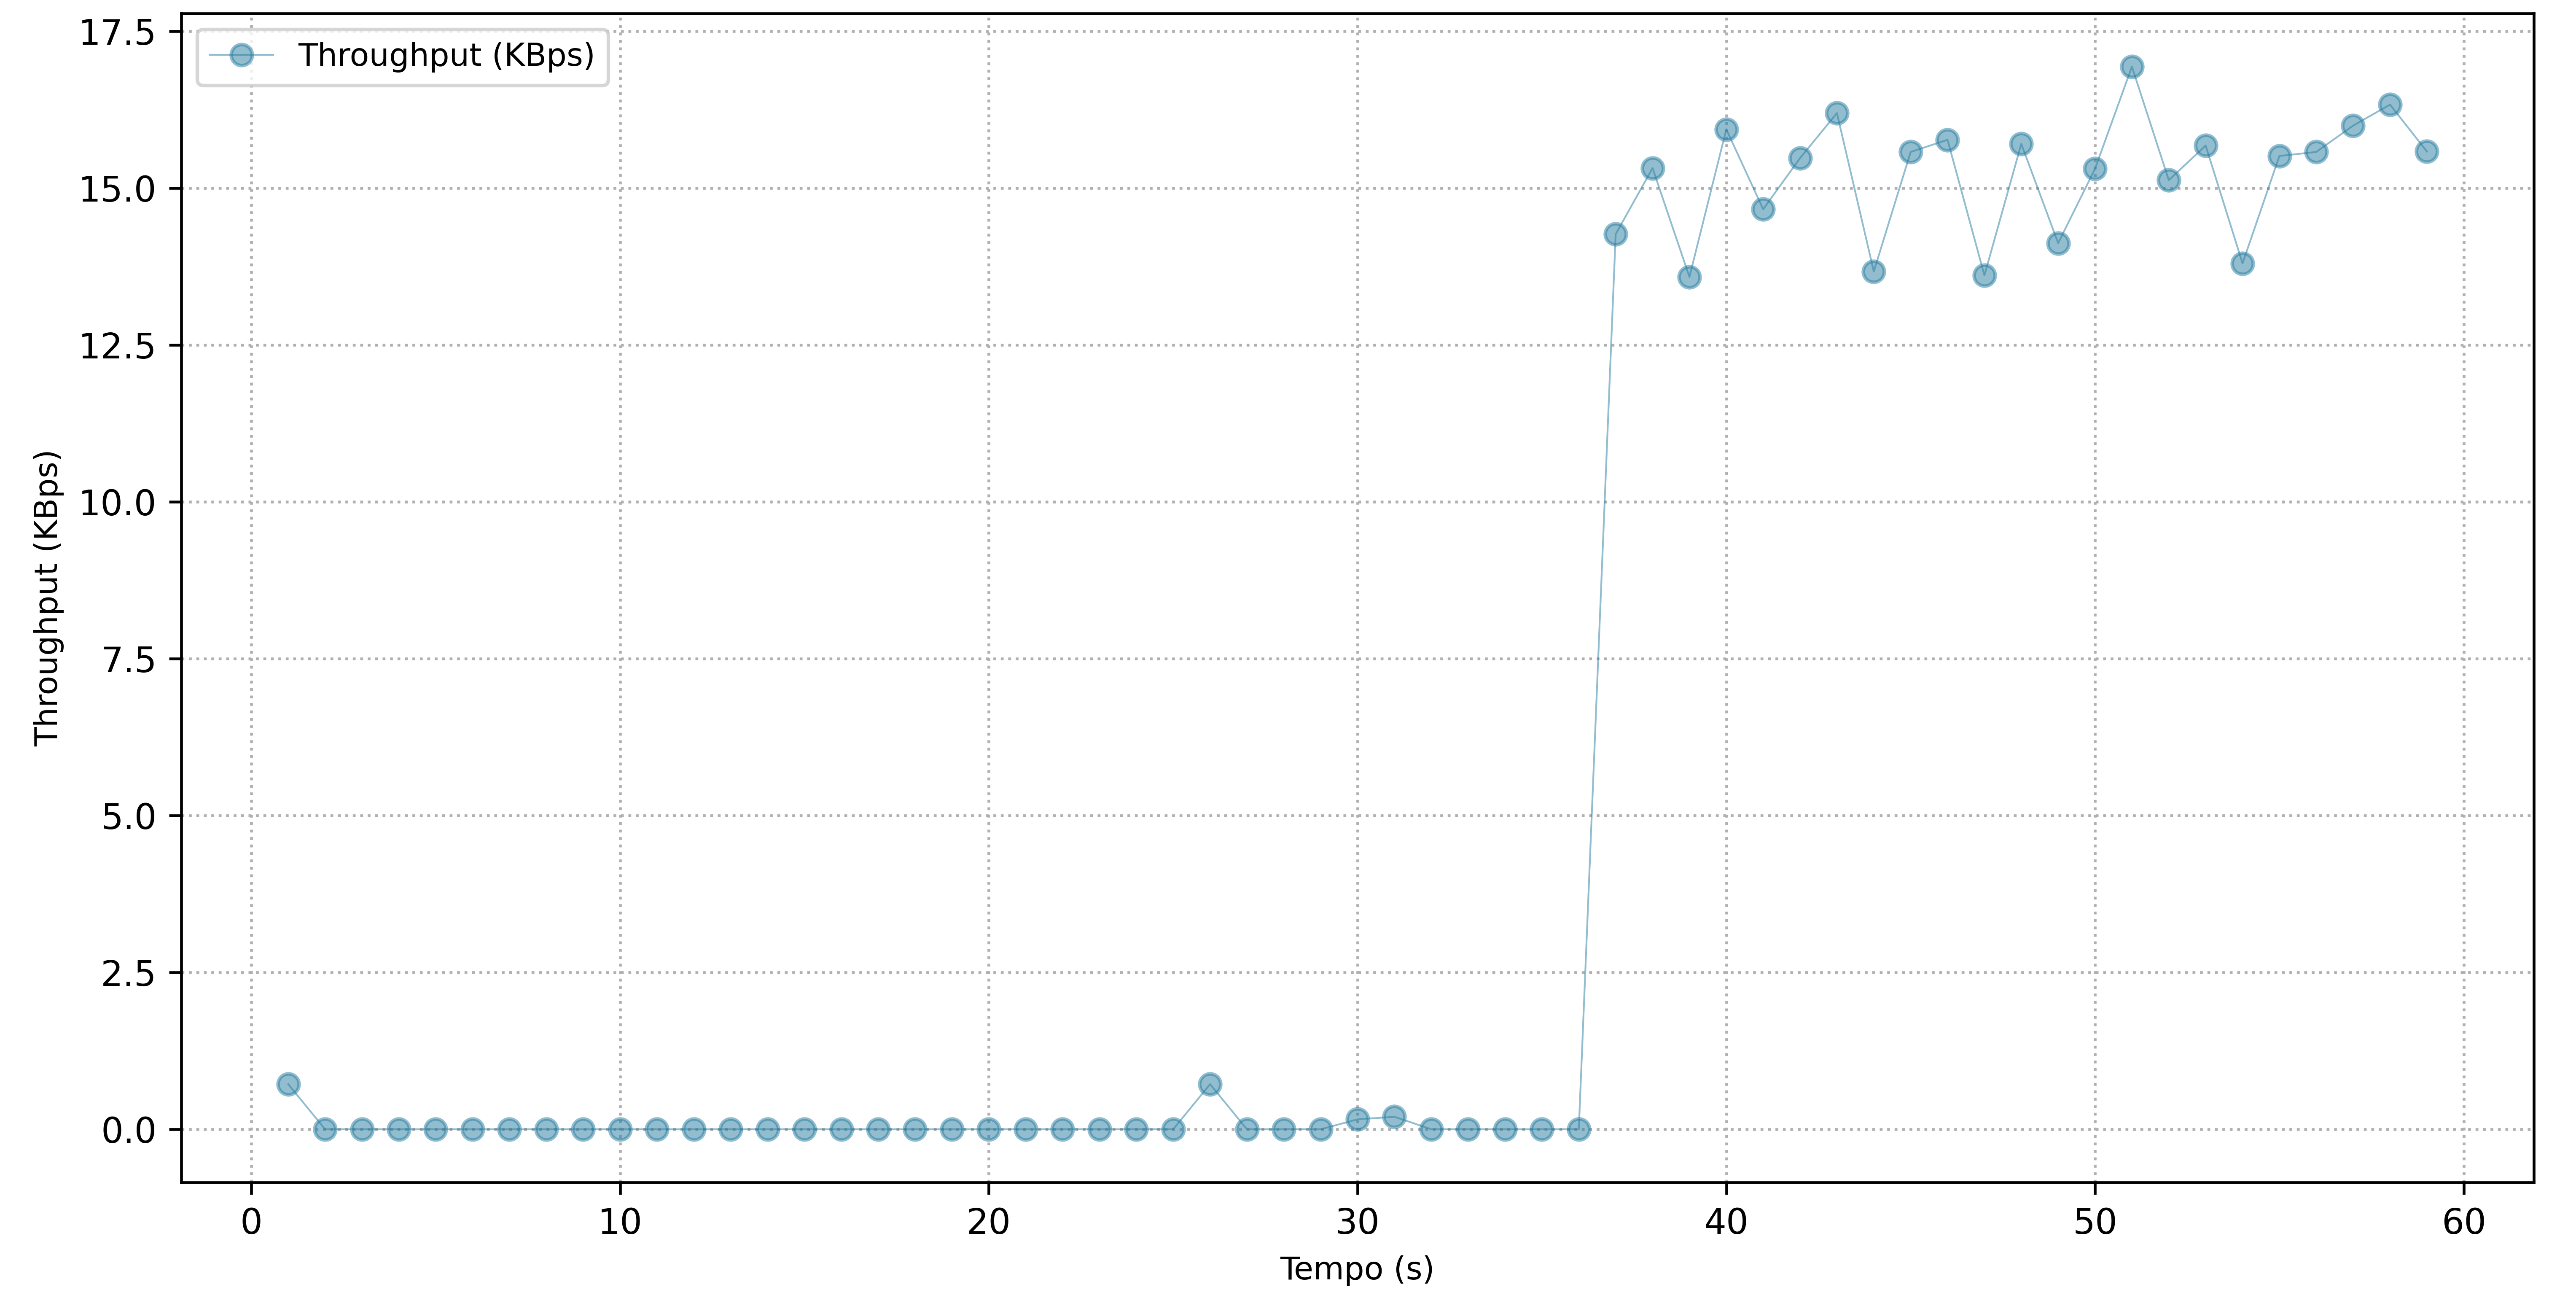
\includegraphics[width=1\textwidth, height=120pt]{USPSC-img/output/cropped/0-normal_local_server-tput.png}
    \end{subfigure}%
    ~ 
    \begin{subfigure}[t]{0.5\textwidth}
        \centering
        \caption{Desempenho}
        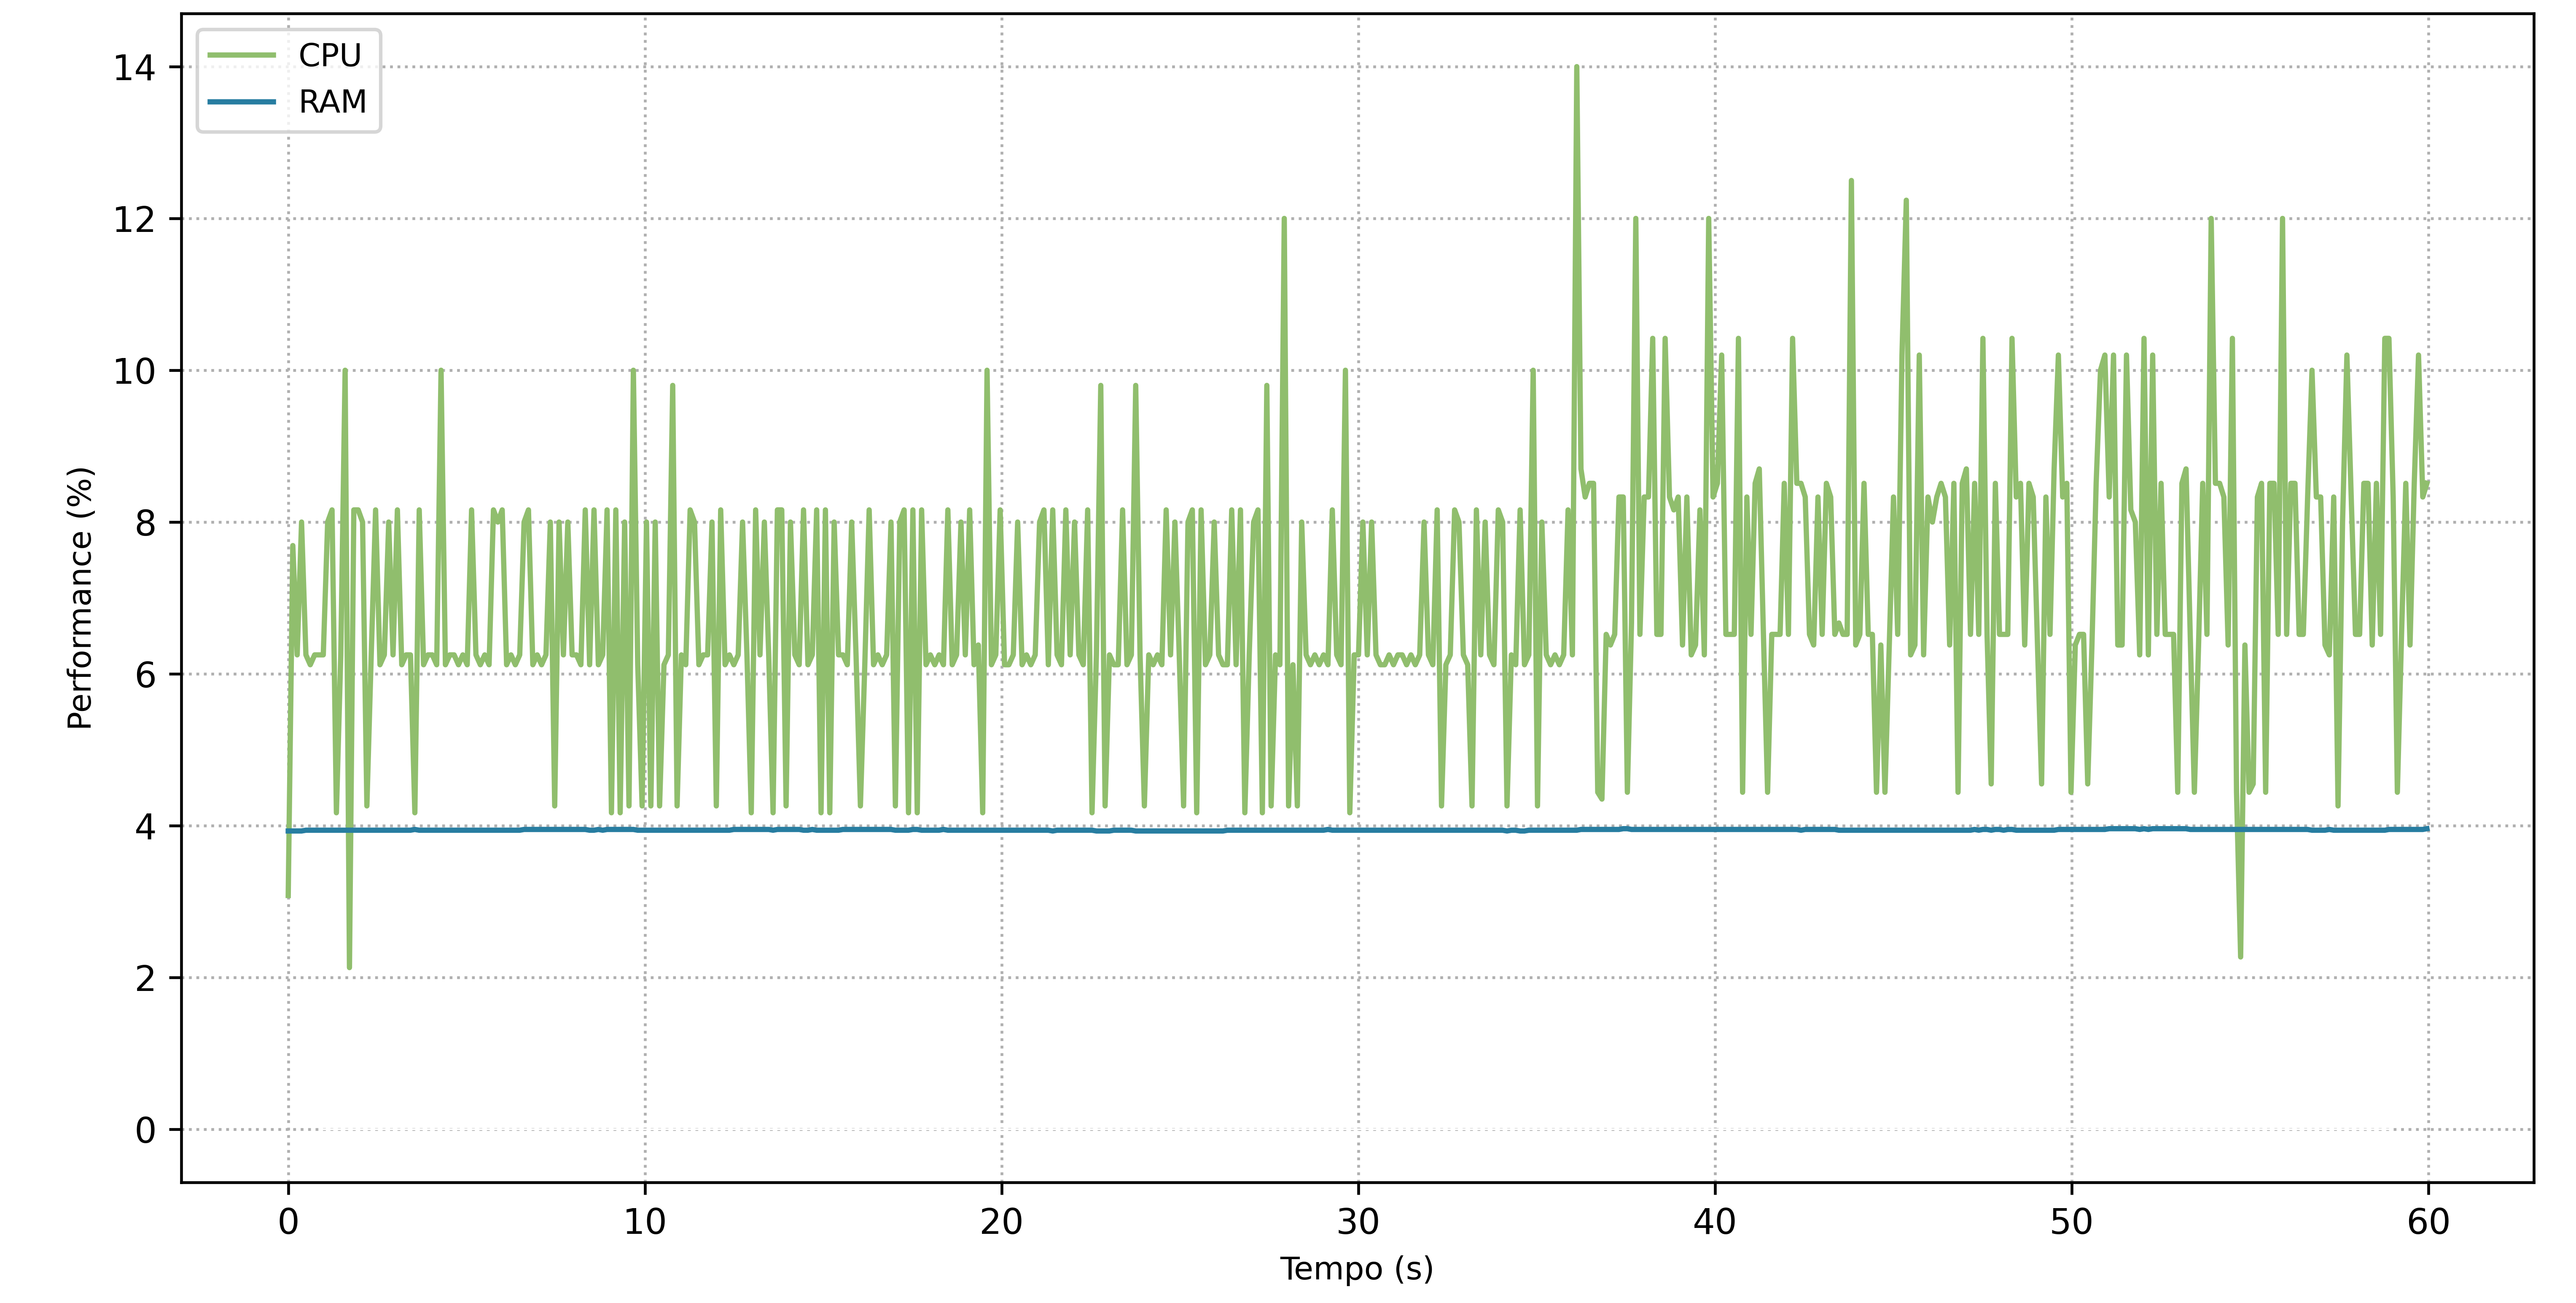
\includegraphics[width=1\textwidth, height=120pt]{USPSC-img/output/cropped/0-normal_local_server-perf.png}
    \end{subfigure}%
    \\
    \begin{subfigure}[t]{0.5\textwidth}
        \centering
        \caption{Pacotes OPC UA}
        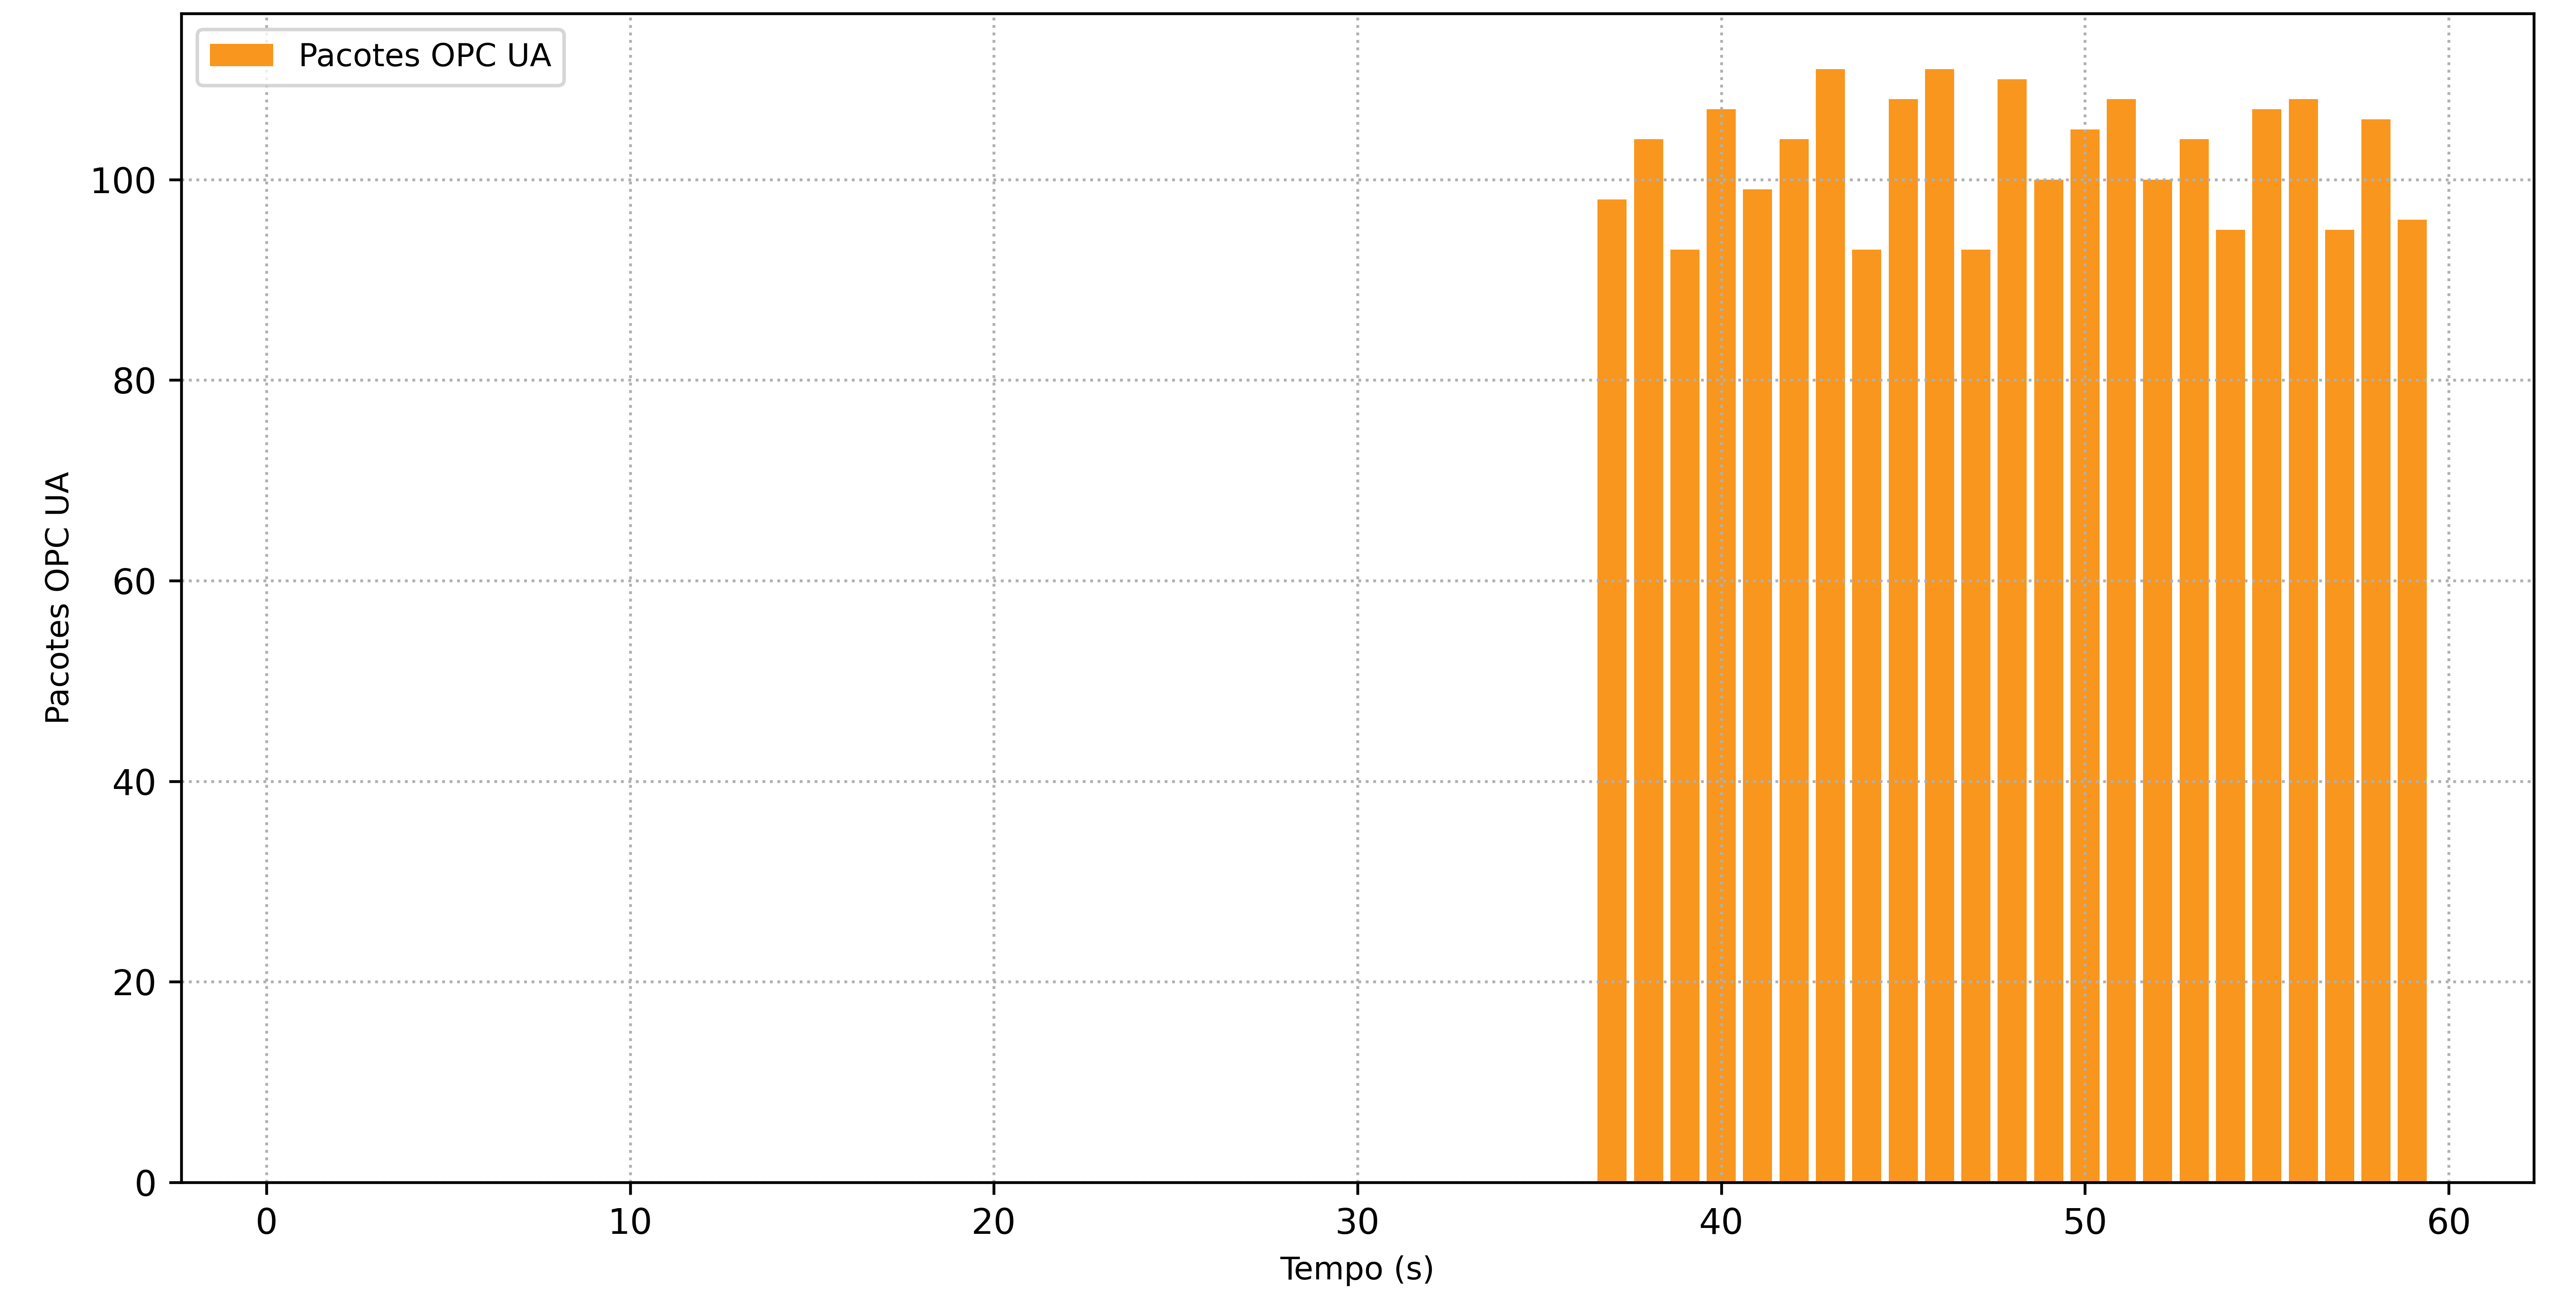
\includegraphics[width=1\textwidth, height=120pt]{USPSC-img/output/cropped/0-normal_local_server-pack.png}
    \end{subfigure}%
    ~
    \begin{subfigure}[t]{0.5\textwidth}
        \centering
        \caption{RTT por pacote}
        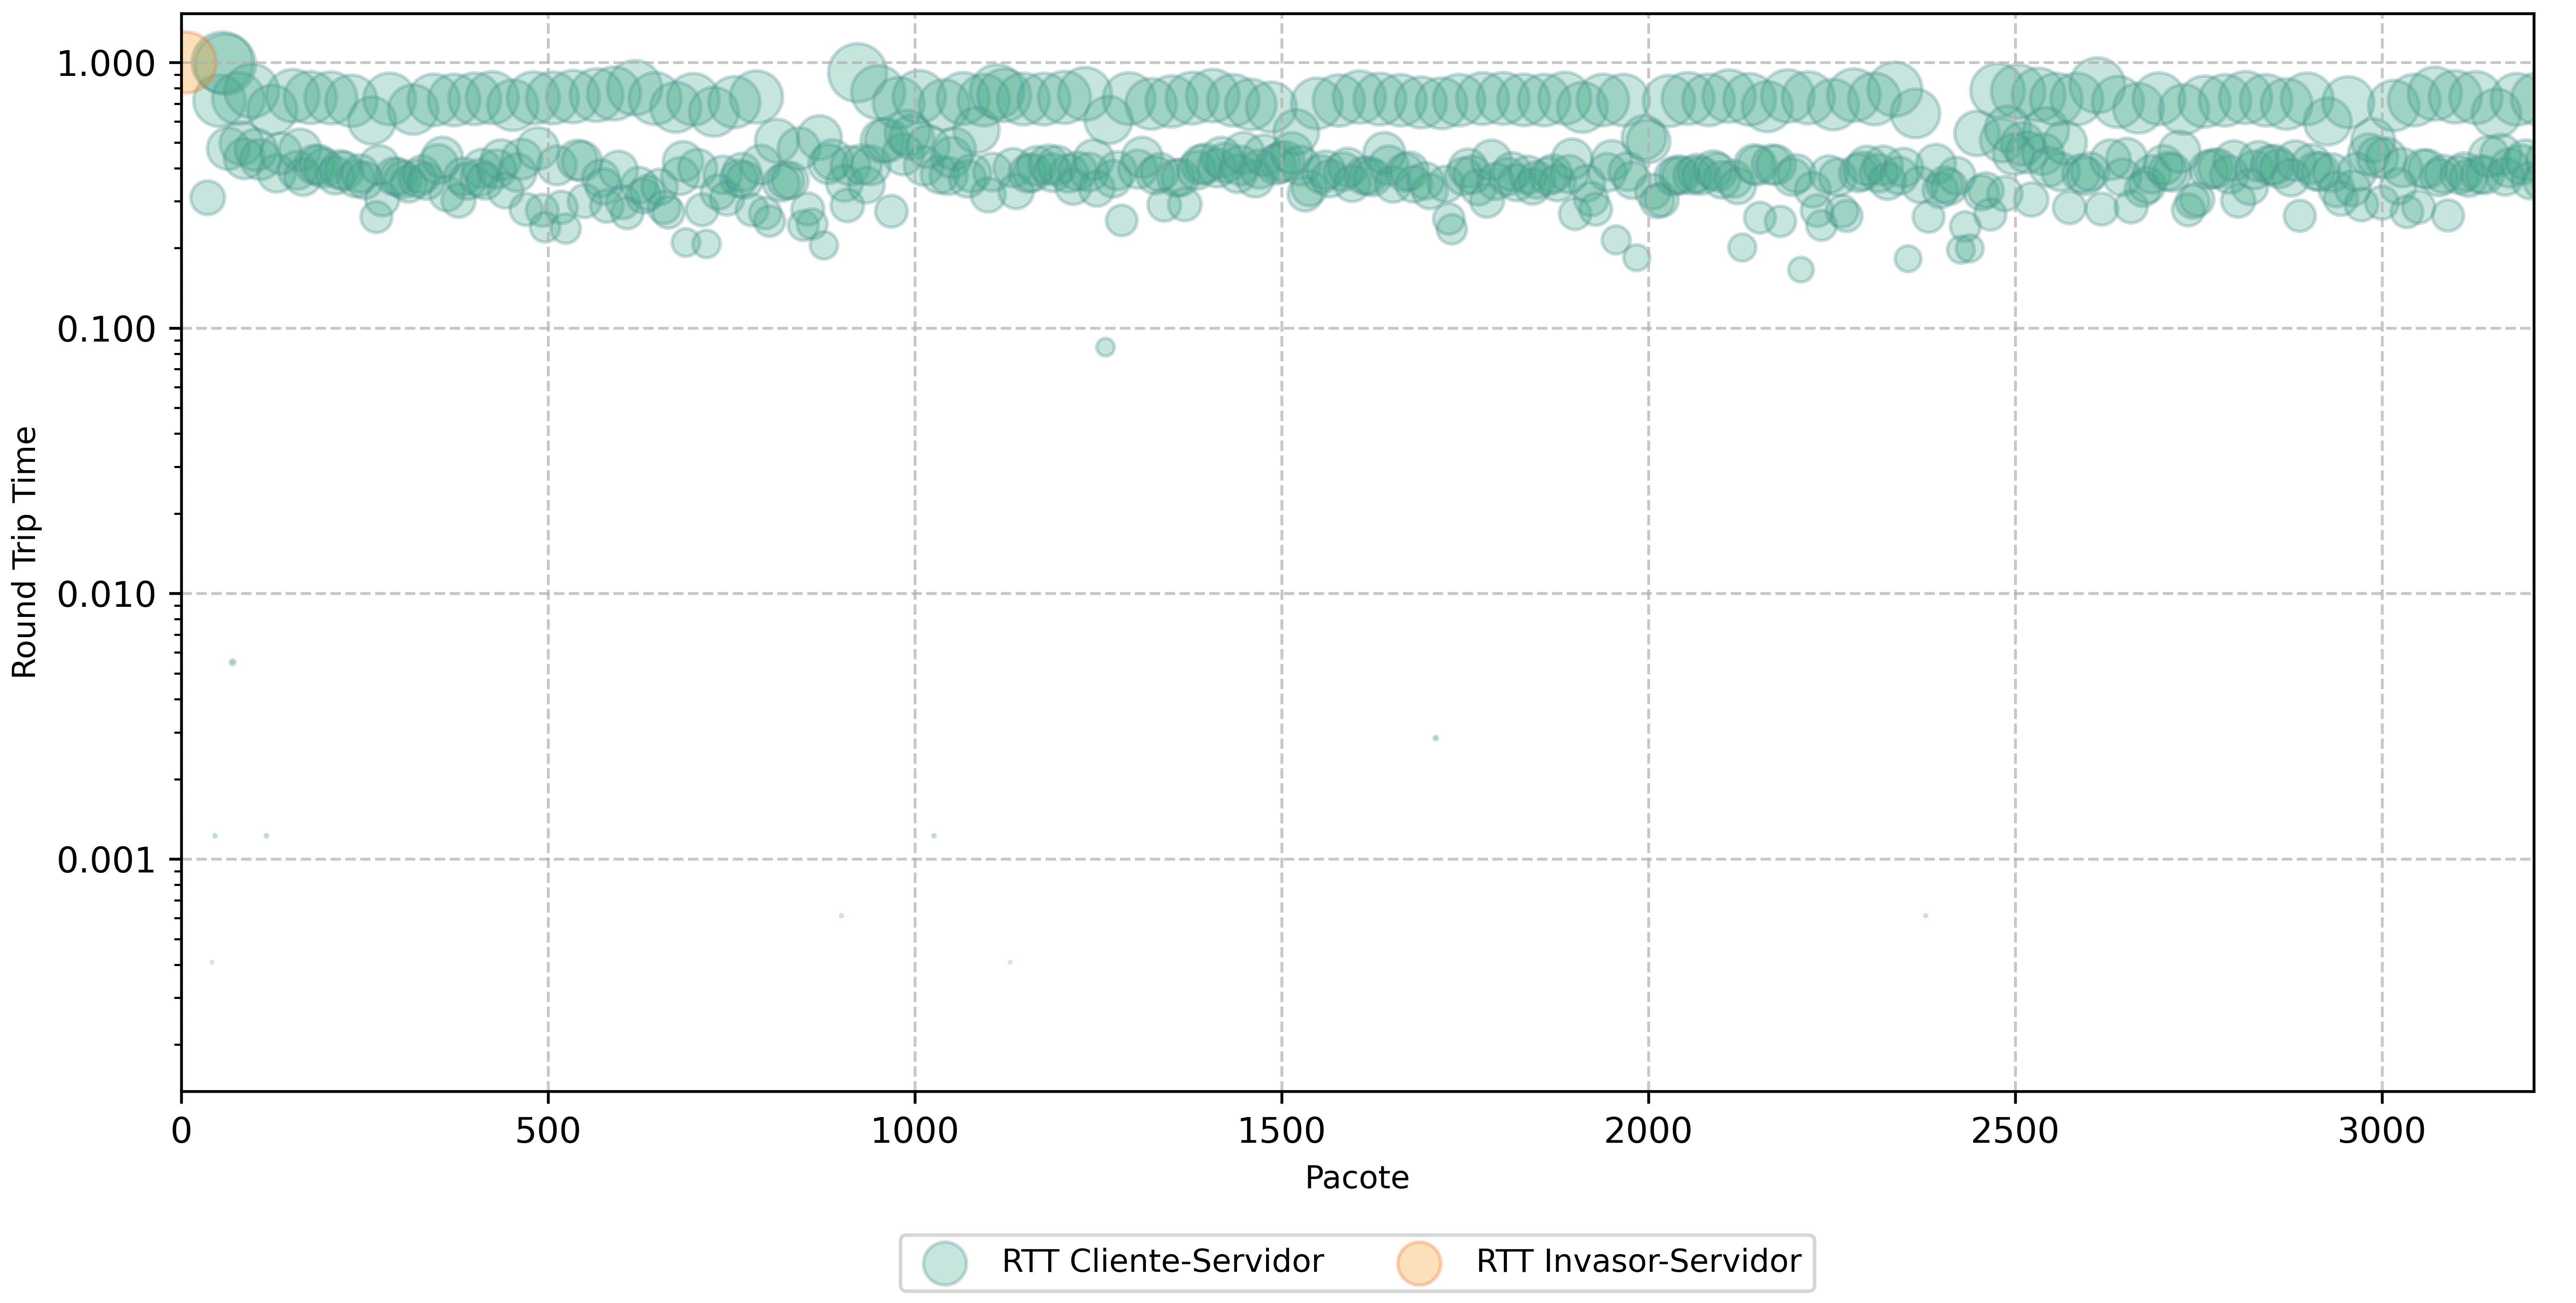
\includegraphics[width=1\textwidth, height=120pt]{USPSC-img/output/cropped/0-normal_local_server-rttp.png}
    \end{subfigure}%
    \legend{Fonte: elaborada pelo autor.}
\end{figure}

Os demais gráficos gerados para os outros cenários podem ser visualizados no \autoref{ap:graficos}.

\section{Análise dos Resultados} \label{sec:analise-resultados}

Nesta seção, são apresentadas as análises dos resultados obtidos a partir dos cenários de ataques cibernéticos executados na bancada experimental. A análise é realizada com base nas métricas de desempenho extraídas dos dados brutos coletados, com o objetivo de avaliar a robustez das redes industriais OPC UA e a variação no desempenho dos componentes ao serem submetidos a tais cenários. Com isso, para organizar melhor as informações, os resultados são divididos em seções que correspondem a cada tipo de ataque

\subsection{\textit{Packet Sniffing}}

Com o auxílio do Wireshark e do Ettercap, este primeiro ataque foi proferido com o objetivo de identificar a presença de vulnerabilidades na rede OPC UA que permitam a interceptação não autorizada de pacotes. Inicialmente, o Ettercap foi empregado para a captura unificada de pacotes, enquanto o Wireshark foi utilizado para a análise detalhada do tráfego de rede. Uma vez que o servidor e o cliente estão conectados, um canal seguro para comunicação é estabelecido. No entanto, o atacante pode explorar vulnerabilidades na rede para interceptar pacotes e obter informações confidenciais, como endereços IP e MAC de todos os dispositivos conectados. No início da captura para o cenário C22, C23 e C24, é possível observar a presença de pacotes de comunicação entre o servidor e o cliente, conforme ilustrado na \autoref{fig:0-sniffing-wireshark}. Note que um filtro foi aplicado para exibir apenas os pacotes de comunicação OPC UA e todos os outros dados foram omitidos nesta visualização. Todo o tráfego relevante relacionado ao protocolo OPC UA apresentado pela \autoref{fig:seqConn} é exposto na análise pelo Wireshark.

\begin{figure}[htbp!]
    \caption{\label{fig:0-sniffing-wireshark}Comunicação interceptada entre o servidor e o cliente OPC UA com modo de segurança `None'}
    \begin{center}
        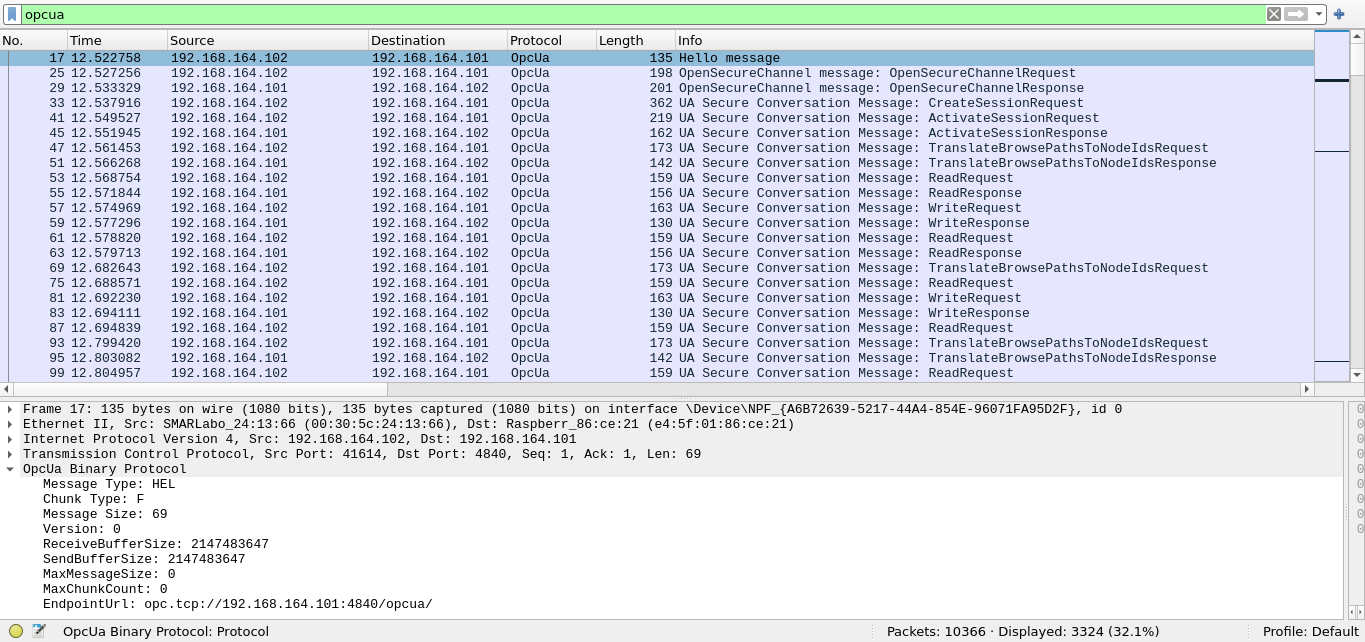
\includegraphics[width=0.972\textwidth]{USPSC-img/0-sniffing-wireshark-filtered-anon.png}
    \end{center}
    \legend{Fonte: elaborada pelo autor.}
\end{figure}

Vale ressaltar que o invasor possui endereço de IP 192.168.164.115, e que está apenas conectado à rede, sem interação física com o servidor (192.168.164.101) ou cliente (192.168.164.102). Para a configuração da comunicação com modo de segurança `None' e `Sign', é possível observar que a capacidade do invasor obter todos os dados sensíveis da comunicação entre o servidor e o cliente, conforme indicado na \autoref{fig:writeRequest}, que representa a coleta do pacote de requisição de escrita (\textit{UA Secure Conversation Message: WriteRequest}) do mesmo valor e nó, do cliente para o servidor.

\begin{figure}[htbp!]
    \centering
    \caption{\label{fig:writeRequest}Informações obtidas pelo invasor com modo de segurança `None' e `Sign'}
    \begin{subfigure}[t]{0.5\textwidth}
        \centering
        \caption{`None'}
        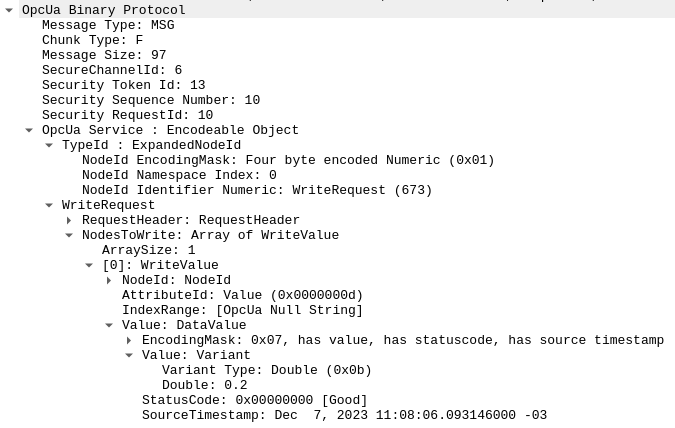
\includegraphics[width=1\textwidth]{USPSC-img/0-sniffing-WriteRequest.png}
    \end{subfigure}%
    ~ 
    \begin{subfigure}[t]{0.5\textwidth}
        \centering
        \caption{`Sign'}
        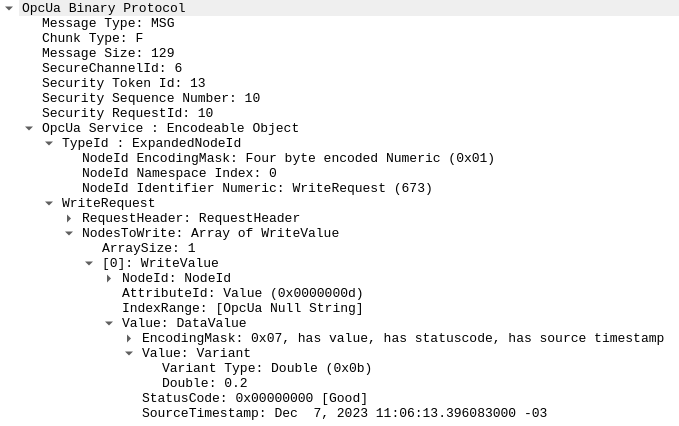
\includegraphics[width=1\textwidth]{USPSC-img/1-sniffing-WriteRequest.png}
    \end{subfigure}%
    \legend{Fonte: elaborada pelo autor.}
\end{figure}

No entanto, ao configurar a comunicação com o modo de segurança `Sign \& Encrypt', o invasor não é capaz de obter informações sensíveis da comunicação entre o servidor e o cliente, pois os dados são, além de assinados, criptografados com políticas de segurança mais robustas, como Basic256Sha256. Assim, para C24, os dados da rede continuam sendo interceptados, mas a comunicação OPC UA não pode ser decifrada, uma vez que todos os pacotes do tipo MSG, com informação \textit{UA Secure Conversation Message: ServiceId [ID]}, possuem o campo de dados \texttt{NodeId EncodingMask} desconhecido.

Portanto, este ataque possui potencial para comprometer a segurança da rede OPC UA ao quebrar a confidencialidade da comunicação, desde que a comunicação seja configurada com modos de segurança mais fracos, como `None' e `Sign'. Tais cenários de ataque evidenciam que, com a utilização de ferramentas simples e acesso ao componente principal da rede, um invasor pode facilmente realizar ataques de captura de pacotes na rede OPC UA, comprometendo dados confidenciais sobre toda a rede. O invasor é capaz de registrar todo o tráfego trocado na rede e, posteriormente, utilizá-lo para outros tipos de ataques, como inserção de pacotes maliciosos (do inglês \textit{packet injection}), DoS, MITM, DDoS, entre outros.

\subsection{\textit{Man in the Middle (MITM)}}

Depois de realizar com sucesso o ataque de \textit{Packet Sniffing}, o invasor terá acesso à uma lista de endereços de todos os dispositivos da rede, além de conhecer informações sensíveis do hospedeiro do servidor OPC UA, incluindo o \texttt{EndpointURI}. Logo, o ataque MITM, pode ser realizado para possibilitar, além da interceptação dos dados, também o controle total da comunicação.

Ambas as técnicas utilizadas para empregar o ataque MITM foram realizadas com sucesso. A execução pela falsificação da tabela ARP, cenários C16, C17 e C18, demonstra que a comunicação é interceptada e redirecionada para o invasor, possibilitando a capturar e modificar os pacotes de dados. A \autoref{fig:0-mitm-wireshark} demonstra a captura de pacotes de comunicação entre o servidor e o cliente, com o invasor atuando como intermediário. Ao comparar com o tráfego apresentado pela \autoref{fig:0-sniffing-wireshark}, é possível observar que o fluxo normal de comunicação é interceptado e redirecionado para o invasor com o endereço MAC \texttt{00:09:5B:A0:5F:F0}.

\begin{figure}[htbp!]
    \centering
    \caption{\label{fig:0-mitm-wireshark}Interceptação de pacotes no ataque MITM com modo de segurança `None'}
    \begin{subfigure}[t]{1\textwidth}
        \centering
        \caption{\texttt{OpenSecureChannelRequest}}
        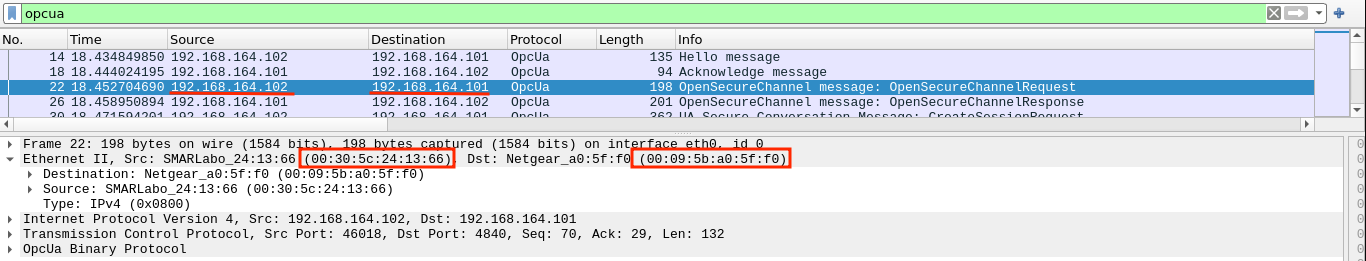
\includegraphics[width=1\textwidth]{USPSC-img/0-mitm-arp_1.png}
    \end{subfigure}%
    \\
    \begin{subfigure}[t]{1\textwidth}
        \centering
        \caption{\texttt{OpenSecureChannelResponse}}
        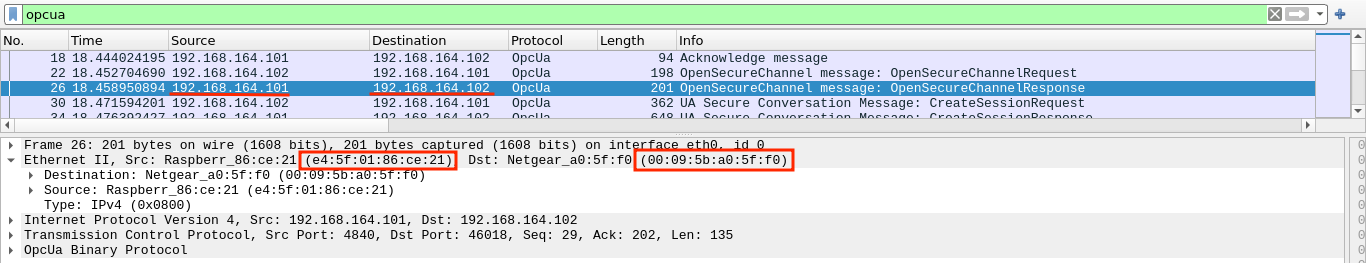
\includegraphics[width=1\textwidth]{USPSC-img/0-mitm-arp_2.png}
    \end{subfigure}%
    \legend{Fonte: elaborada pelo autor.}
\end{figure}

Inicia-se com a etapa de hand-shake entre os agentes, com a saudação do cliente, seguida por um reconhecimento do servidor. Em seguida, o cliente envia uma solicitação \textit{OpenSecureChannelRequest}, à qual o servidor responde com uma \textit{OpenSecureChannelResponse}. Após essa etapa, é criado um \textit{SecureChannel}, e o cliente envia uma \textit{CreateSessionRequest}, que é respondida pelo servidor com uma \textit{CreateSessionResponse}. Uma vez que a sessão é criada, cliente e servidor se ativam usando \textit{ActivateSessionRequest} e \textit{ActivateSessionResponse}. A partir desse ponto, quando o cliente tenta acessar qualquer informação do servidor, observa-se as mensagens \textit{ReadRequest} e \textit{ReadResponse}.

No ataque MITM pelo roubo de portas, cenários C19, C20 e C21, um aumento no \texttt{throughput} é observado, alcançando valores dez vezes maior que o executado pela falsificação da tabela ARP. Essa elevação ocorre devido ao processo de roubo de portas, cuja rede é inundada com pacotes ARP para saturar a tabela ARP do servidor, forçando-o a redirecionar o tráfego para o invasor. Em média, 99.3\% dos pacotes nesses cenários são provenientes do \textit{broadcast} ARP. No entanto, uma vez que esta técnica é empregada com sucesso e a interceptação efetuada, nota-se que a comunicação não é realizada através do invasor, mas sim diretamente entre o servidor e o cliente com a replicação desta para a porta roubada pelo invasor.

A partir de ambas as tecnicas empregadas, nota-se algumas informações confidenciais são obtidas pelo invasor, como o \texttt{EndpointURI} do servidor, o \texttt{SecurityPolicy} e o \texttt{SecurityMode} utilizados na comunicação,  as informações que o servidor OPC UA obtém da rede do chão de fábrica em um ambiente industrial em tempo real. No entanto, vale ressaltar que o invasor não é capaz de decifrar os pacotes de comunicação para o ambiente configurado com o maior nível de segurança (`Sign \& Encrypt') e com políticas de segurança atualizadas. Supõe-se também que para execução deste ataque o invasor tenha acesso físico à rede, o que não deve ser comum em ambientes industriais.

\subsection{\textit{Denial of Service (DoS)}}

Nesta seção, são apresentados os resultados obtidos a partir dos cenários de ataques de negação de serviço (DoS) executados na bancada experimental utilizando cinco técnicas distintas. O objetivo desses ataques é avaliar a capacidade da rede industrial OPC UA de resistir a sobrecargas de tráfego e a variação no desempenho dos componentes ao serem submetidos a tais cenários.

\subsubsection*{\underline{Inundação TCP/IP}}

A execução do ataque pela inundação TCP/IP (cenários C7, C8 e C9) consistiu na varredura inicial da rede para identificar dispositivos e serviços ativos, utilizando Nmap. Os resultados revelaram a presença de um servidor OPC UA em execução e sua respectiva porta aberta para essa comunicação. Isso é suficiente para que o próximo passo seja executado: inundação de pacotes SYN pela comunicação TCP/IP.

Os resultados obtidos para esses cenários indicam que a rede é altamente vulnerável a ataques de inundação TCP/IP, com um aumento significativo no \texttt{throughput} e na taxa de pacotes por segundo. O servidor OPC UA é sobrecarregado com a alta carga de tráfego, resultando em um aumento no uso da CPU e na degradação do desempenho do sistema. 

\subsubsection*{\underline{Loop infinito na cadeia de certificados}}

\subsubsection*{\underline{Chamada da função Dereference nula}}

\subsubsection*{\underline{Abertura de múltiplos canais seguros}}

\subsubsection*{\underline{Tradução do caminho de navegação}}

\section{Propostas de Melhorias e Mitigações} \label{sec:melhorias-mitigacoes}

\subsection{Recomendações para Comunicações Seguras com o Protocolo OPC UA}

Como resultado de uma série de testes realizados em conformidade com os padrões de segurança, foram identificadas e resumidas as seguintes recomendações para o uso de comunicações seguras com o protocolo OPC UA:

\begin{itemize}
    \item \textbf{Operação no "SecurityMode"}: É essencial selecionar os modos `Sign' ou `Sign \& Encrypt'. Esses modos garantem que, no nível da aplicação, a autenticação seja obrigatória. O modo de segurança `None' não oferece proteção alguma! O modo de segurança `Sign \& Encrypt' é utilizado para proteger a integridade dos dados e sua confidencialidade.
    \item \textbf{Escolha dos Algoritmos Criptográficos}: Deve-se selecionar `Basic256Sha256' como a \textit{Security Policy}, desde que os clientes com os quais o servidor interage suportem essa política. Políticas de segurança que utilizam algoritmos obsoletos, como `SHA-1', não devem ser utilizadas.
    \item \textbf{Autenticação de Usuários}: O login no servidor UA com um ID `anônimo' deve ser utilizado apenas ao acessar recursos não críticos, pois, nesse caso, não é possível rastrear quem está alterando os dados ou a configuração. Hackers podem explorar essas recomendações para usar o OPC UA com um ID seguro para ler ou escrever dados de maneira não autorizada. Isso pode ocorrer se a restrição dos direitos de trabalho com o identificador `anônimo' não for configurada adequadamente.
    \item \textbf{Armazenamento de Certificados e Chaves Privadas}: As chaves privadas ou arquivos de certificado utilizados não devem ser armazenados em um sistema de arquivos não criptografado. Para esse propósito, devem ser usados armazenamentos especiais de certificados do sistema operacional e suas capacidades para definir direitos de acesso. Recomenda-se o uso de TPMs (\textit{Trusted Platform Modules}) ou hardware seguro externo, como tokens de autenticação USB, para armazenar certificados e/ou chaves privadas.
    \item \textbf{Uso de Certificados}: Conexões que não fornecem certificados confiáveis não são permitidas. Certificados autoassinados requerem verificação adicional. Se os certificados não forem autoassinados, é necessário o estabelecimento de uma autoridade certificadora, e os certificados dessa autoridade devem ser assinados de forma independente ou por outra autoridade certificadora. As autoridades certificadoras podem ser multinível.
    \item \textbf{Gestão e Manutenção de Certificados}: Recomenda-se o uso de listas de confiança de certificados e listas de revogação de certificados para gerenciar apenas certificados válidos. Essas listas são criadas por usuários ou processos confiáveis e devem ser atualizadas regularmente.
\end{itemize}

\subsection{Na Rede}

MITM:

Port stealing Port stealing - countermeasures - countermeasures
n YES - port security on the switch - port security on the switch
n NO - static ARP - static ARP

ARP poison - countermeasures - countermeasures
n YES - passive monitoring (arpwatch) - passive monitoring (arpwatch)
n YES - active monitoring (ettercap) - active monitoring (ettercap)
n YES - IDS (detect but not avoid) - IDS (detect but not avoid)
n YES - Static ARP entries entries (avoid it) (avoid it)
n YES - Secure-ARP (public - Secure-ARP (public key auth)
n NO - Port security security on the on the switch
n NO - anticap anticap, antidote, , antidote, middleware middleware approach approach

% \section{Resultados Esperados}

% Na busca por aprimorar a cibersegurança dos sistemas de controle e automação industrial por meio de uma análise meticulosa das vulnerabilidades em redes OPC UA, é imperativo delinear os resultados esperados da metodologia aplicada no presente trabalho. As expectativas de resultados estão fundamentadas em uma avaliação abrangente da robustez da rede e variações no desempenho dos controladores ao serem submetidos aos cenários de ataque cibernético apresentados na \autoref{sec:attacks}.

% Primeiramente, no que se refere à simulação de ataques de \textit{Packet Sniffing}, espera-se que as redes OPC UA demonstrem um alto nível de resistência à interceptação não autorizada de pacotes, decorrente do modo de segurança inerente ao protocolo utilizado. O maior nível de proteção é apresentado pelo modo \textbf{Sign\&Encrypt}, no qual inclui recursos de criptografia e autenticação. Consequentemente, as informações trocadas entre cliente e servidor OPC UA permanecem confidenciais, íntegras e disponíveis (CIA), garantindo assim a segurança da rede.

% Em segundo lugar, no contexto de ataques do tipo \textit{Man-in-the-Middle} (MITM), é imperativo considerar a detecção e prevenção destas intrusões, também com uma dependência significativa do modo de segurança selecionado. Semelhante ao cenário de ataque anterior, uma configuração que priorize o mais alto nível de segurança e a seleção adequada de políticas de criptografia devem, a princípio, proteger a rede OPC UA contra ataques MITM perpetrados por um possível Elemento Invasor. Entretanto, em situações que existam vulnerabilidades conhecidas na rede e em sua configuração, como a utilização do modo \textbf{None}, um elemento não confiável pode explorar tais fragilidades para corromper a tabela ARP (\textit{ARP Spoofing}), permitindo a interceptação das informações transmitidas entre o cliente e o servidor. Além disso, esse invasor pode modificar potencialmente dados por meio da inserção de algum \textit{malware}.

% Por fim, no que diz respeito a ataques de negação de serviço (DoS), é importante considerar que os resultados esperados podem diferir dos observados nos ataques mencionados anteriormente, dependendo da capacidade da rede e de processamentos dos componentes \textit{hosts} do servidor OPC UA. Antecipa-se que, embora o ambiente experimental desenvolvido compreenda apenas alguns dispositivos de redes e não incorpore preocupações com a capacidade de comunicação, a correta avaliação dos dados capturados nos cenários simulados deverá evidenciar que esse ataque pode prejudicar a troca de mensagens ao esgotar os recursos de uma rede com grande composição. Estima-se, ainda, que os danos sejam mais significativos quando se utiliza o modo de segurança \textbf{Sign\&Encrypt} e quando o inunda com os pacotes referentes a validações de certificado e ao processo de criptografia.

% Além disso, a pesquisa se esforça para fornecer informações valiosas sobre vulnerabilidades potenciais que podem ser expostas durante o processo de experimentação. Estas prospecções, caso confirmadas, auxiliam em avanços futuros do protocolo OPC UA e de sistemas IACSs, fortalecendo ainda mais a robustez destes e resistência contra ameaças cibernéticas em constante evolução.


\chapter{Considerações Finais} \label{cap:conclusao}

    O presente trabalho teve como objetivo principal analisar as vulnerabilidades presentes nas redes industriais que utilizam o protocolo OPC UA, abordando suas implicações de segurança e os riscos associados ao seu uso no contexto da Indústria 4.0.

\section{Conclusões}

    A primeira etapa da pesquisa consistiu em uma revisão detalhada sobre a arquitetura do OPC UA, abordando seus requisitos fundamentais, o funcionamento dos clientes e servidores OPC UA, bem como os procedimentos necessários para o estabelecimento de canais de comunicação seguros entre essas entidades. A partir dessa revisão, foi possível identificar diversas vulnerabilidades do protocolo, incluindo ataques de negação de serviço (DoS), escuta clandestina, falsificação de mensagens, alteração de mensagens, repetição de mensagens e sequestro de sessões.

    Em seguida, o trabalho propôs a implementação de um ambiente de testes baseado na arquitetura OPC UA, utilizando dispositivos Raspberry Pi para simular um cliente e um servidor OPC UA. Inicialmente, foi adotada a configuração padrão do protocolo, com a política de segurança definida como ``None''. No cenário experimental, três tipos de ataques cibernéticos foram realizados: sniffing de pacotes, ataque ``man in the middle'' (MITM) e ataque de negação de serviço (DoS). O ataque MITM, por exemplo, demonstrou a vulnerabilidade à comprometer a confidencialidade, a autorização e a autenticação da comunicação, evidenciando a dependência do tipo de configuração do open62541. Já os ataques DoS, realizados por meio de TCP-SYN Flood e TCP Anomalies, revelaram o impacto significativo desses ataques no uso da CPU do servidor OPC UA, com o TCP-SYN causando maior sobrecarga nos recursos computacionais.

    Além dos ataques, o trabalho também se concentrou em métodos de detecção simples, voltados para a identificação de tais ataques a partir do lado da vítima, utilizando ferramentas como Wireshark e ARP. Essa abordagem permitiu a identificação de padrões e anomalias associadas a ataques cibernéticos, proporcionando uma base para a prevenção e mitigação de falhas no sistema.

    As conclusões extraídas deste trabalho destacam a complexidade e a vulnerabilidade das redes industriais que utilizam o protocolo OPC UA. Embora amplamente adotado em diversos setores industriais, o protocolo apresenta sérias falhas de segurança que podem comprometer a integridade e a confidencialidade das comunicações. As vulnerabilidades identificadas neste estudo podem ter impactos graves nas operações industriais, especialmente em um contexto no qual a automação e a interconexão de dispositivos são cada vez mais comuns. Entre as principais lições aprendidas, destaca-se a urgência em melhorar a segurança do protocolo OPC UA, por meio não apenas da adoção de configurações mais robustas, mas também pela implementação de métodos eficazes de detecção e mitigação de ataques.

    Este estudo também evidenciou a necessidade de continuar o desenvolvimento de soluções mais seguras e resilientes para a Indústria 4.0, destacando a relevância do OPC UA não apenas como protocolo de comunicação, mas como um elemento crucial para a integração da tecnologia operacional com a tecnologia da informação. O crescimento da Internet das Coisas Industrial (IIoT) e a crescente dependência de redes interconectadas tornam ainda mais urgente a proteção dessas infraestruturas contra ameaças cibernéticas. Portanto, os resultados obtidos neste trabalho não apenas contribuem para a compreensão das vulnerabilidades do OPC UA, mas também abrem caminho para futuras investigações e melhorias na segurança das redes industriais.

    Finalmente, este estudo reforça a importância de adotar uma abordagem proativa na análise e mitigação de riscos em redes industriais, com o objetivo de garantir a continuidade operacional, a proteção de dados e a integridade das infraestruturas críticas.

\section{Trabalhos Futuros}

    Este trabalho abordou uma análise aprofundada da arquitetura do OPC UA e a identificação de vulnerabilidades associadas a esse protocolo nas redes industriais, com ênfase nas ameaças cibernéticas e suas contramedidas. No entanto, diversas áreas ainda podem ser exploradas no futuro, tanto para aprofundar o entendimento das vulnerabilidades atuais quanto para aprimorar a segurança na implementação do OPC UA em ambientes industriais.

    Uma direção promissora para pesquisas futuras consiste na integração do OPC UA com redes Time-Sensitive Networking (TSN). O TSN tem o potencial de garantir comunicação em tempo real em redes industriais, o que é crucial para sistemas de automação. Embora os padrões IEEE 802.1, como IEEE 802.1AS e IEEE 1588 v2, já ofereçam suporte à tecnologia, a introdução de Time Division Multiple Access (TDMA) pode criar novas superfícies de ataque, demandando o desenvolvimento de soluções de segurança específicas para essa integração. A pesquisa sobre a aplicação de estratégias de filtragem, como o P802.1Qci, e a possibilidade de criptografia e autenticação das mensagens (padrão IEEE 802.1.AEcg) pode ser uma importante linha de investigação para garantir a confidencialidade e a proteção das informações em um ambiente TSN.

    Além disso, a ampliação da testagem em larga escala de redes OPC UA pode gerar contribuições significativas. A análise do impacto de ataques DoS em redes maiores, com um número ampliado de clientes e servidores, permitirá avaliar o comportamento da segurança do OPC UA em cenários mais complexos. A pesquisa pode explorar também a segmentação da rede, verificando se ataques em partes da rede podem ser contidos sem afetar o desempenho geral da rede OPC UA.

    Outras possibilidades de pesquisa incluem a implementação de ambientes de testes mais diversificados, nos quais diferentes tipos de ataques possam ser simulados em redes industriais que utilizam o protocolo OPC UA. Uma linha promissora de investigação seria a aplicação de sistemas de detecção de intrusão (IDS) baseados em aprendizado de máquina, como modelos híbridos que combinam diferentes metodologias para aprimorar a precisão e eficiência na identificação de ataques em tempo real. A aplicação de técnicas de aprendizado de máquina, como redes neurais artificiais e máquinas de vetores de suporte, para detectar anomalias e prever intrusões, representaria um avanço importante na segurança de redes industriais.

    Por fim, no contexto da Indústria 4.0, onde a convergência entre Tecnologia da Informação (IT) e Tecnologia Operacional (OT) é cada vez mais relevante, é fundamental estudar como essa convergência pode ser aplicada ao OPC UA e como as soluções de segurança podem ser adaptadas para enfrentar os desafios de um mundo interconectado e de rápida evolução. Isso envolve a implementação de protocolos mais robustos e a adoção de novas metodologias para garantir a integridade e a segurança das redes de comunicação industriais.

\subsection{Reflexões Finais}

    O desenvolvimento deste projeto, intitulado ``Análise de Vulnerabilidades em Redes Industriais OPC UA'', proporcionou uma visão abrangente dos desafios e das possibilidades no campo da segurança cibernética no contexto de um dos protocolos mais utilizados para comunicação em redes industriais. O estudo teve como objetivo identificar as vulnerabilidades nas redes que utilizam o protocolo OPC UA, propondo um método eficaz de detecção de intrusões por meio de técnicas de aprendizado de máquina. Durante a execução do projeto, foram analisadas as especificidades do protocolo, suas deficiências em termos de segurança e as ameaças cibernéticas que podem comprometer a integridade e confidencialidade dos dados e sistemas críticos.

    As redes industriais têm se tornado alvos cada vez mais atraentes para cibercriminosos, devido à crescente digitalização e interconexão de sistemas operacionais e de automação. A segurança cibernética dessas redes deve, portanto, ser considerada uma prioridade em qualquer processo de transformação digital. O OPC UA, embora apresente grandes avanços em termos de segurança, como criptografia e autenticação robustas, ainda permanece vulnerável a uma variedade de ataques, como negação de serviço (DoS) e invasões de dados. O uso crescente de ferramentas de inteligência artificial e aprendizado de máquina tem permitido o desenvolvimento de sistemas de detecção de intrusão (IDS) mais sofisticados, capazes de realizar análises preditivas e mitigar incidentes antes que danos irreparáveis ocorram.

    Durante o desenvolvimento deste projeto, observou-se que o uso de técnicas de aprendizado de máquina, especialmente para a detecção de anomalias no tráfego de rede, mostra grande potencial para melhorar a segurança das redes OPC UA. No entanto, é importante destacar que o treinamento de modelos de aprendizado de máquina em redes industriais é um processo complexo e desafiador, devido à escassez de amostras de tráfego anômalo e à dificuldade de capturar comportamentos raros, mas potencialmente prejudiciais, dos atacantes. Esses desafios precisam ser considerados para a implementação real de sistemas de detecção em ambientes de produção, onde a estabilidade e continuidade dos serviços são essenciais.

    Além disso, o estudo das vulnerabilidades revelou a necessidade urgente de estratégias de defesa mais integradas, levando em consideração não apenas os aspectos técnicos do protocolo, mas também as práticas organizacionais e políticas de segurança. Para garantir a segurança das redes industriais, é imprescindível uma abordagem holística, que envolva desde a formação de profissionais qualificados até a implementação de metodologias de defesa resilientes e adaptativas.

    Por fim, a pesquisa realizada neste trabalho, embora tenha abordado aspectos cruciais da segurança em redes OPC UA, deixou claro que o campo da segurança cibernética em ambientes industriais ainda está em fase de desenvolvimento. A rápida evolução das tecnologias, o surgimento de novos tipos de ameaças e a crescente complexidade dos sistemas exigem que a pesquisa continue, com o objetivo de fornecer soluções mais robustas e adaptáveis. Este projeto contribui para a base de conhecimento existente e abre portas para novas pesquisas que possam aprimorar a compreensão dos riscos e das contramedidas aplicáveis às redes industriais do futuro.

% \begin{figure}[H]
%     \begin{center}
%         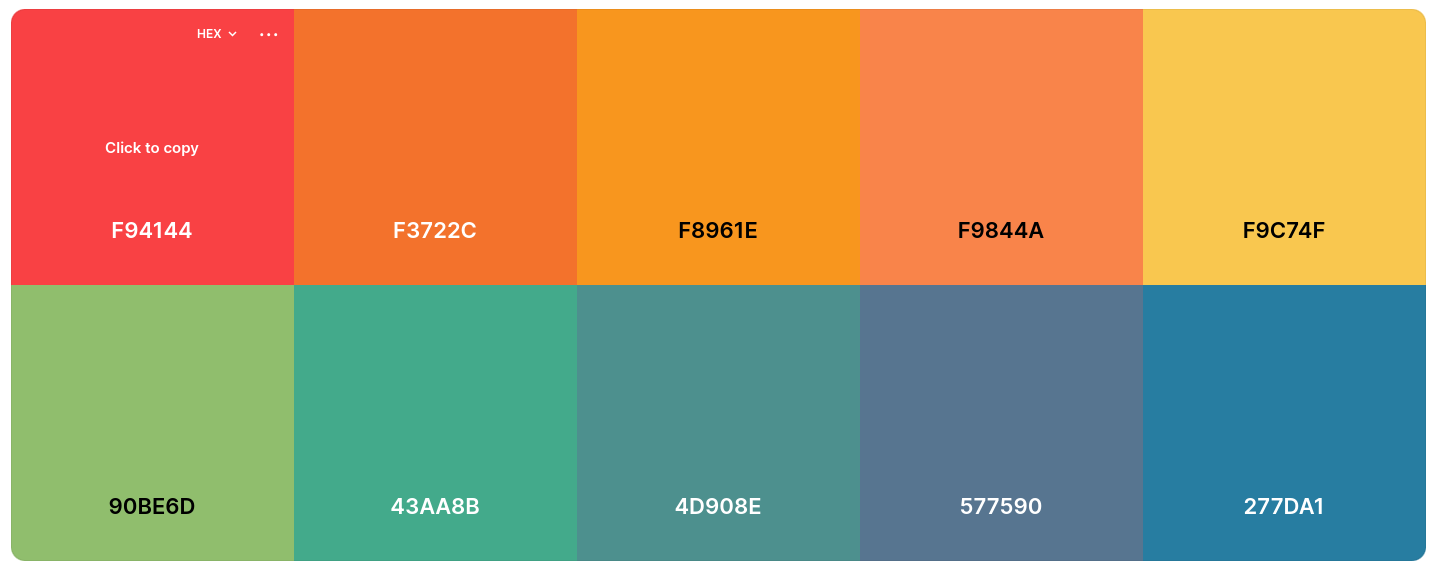
\includegraphics[width=1\textwidth]{USPSC-img/masterPalette.png}
%         \url{https://coolors.co/palette/f94144-f3722c-f8961e-f9844a-f9c74f-90be6d-43aa8b-4d908e-577590-277da1}
%     \end{center}
% \end{figure}

% \chapter{Cronograma Proposto} \label{cap:cronograma}

Para auxiliar no planejamento e execução dos objetivos do presente trabalho, as atividades elaboradas para cumprimento são dispostas no \autoref{qdr:metas} e o cronograma proposto para o cumprimento destas metas, no \autoref{qdr:cronograma}, permitindo antecipar e mitigar eventuais desvios ou atrasos.

    \begin{quadro}[htbp]
        \setlength\tabcolsep{2pt}
        \renewcommand{\arraystretch}{1.3}
        \caption{Metas estabelecidas para a pesquisa}
        \label{qdr:metas}
        \centering
        \begin{tabular}{
            |>{\centering\arraybackslash}m{0.105\textwidth}
            |>{\raggedright\arraybackslash}m{0.86\textwidth}
        |} \hline
            \textbf{Metas} & \multicolumn{1}{c|}{\textbf{Descrição}} \\ \hline
            1 & Pesquisa bibliográfica \\ \hline
            2 & Projeto e implementação do ambiente de teste para coleta de dados \\ \hline
            3 & Análise e escolha dos ataques cibernéticos \\ \hline
            4 & Implementação dos ataques na bancada experimental \\ \hline
            5 & Dissertação para exame de qualificação \\ \hline
            6 & Coleta e interpretação dos dados \\ \hline
            7 & Análise dos ataques e \index{Vulnerabilidade}vulnerabilidades em redes industriais \index{OPC UA}OPC UA \\ \hline
            8 & Verificação de desempenho e validação dos resultados \\ \hline
            9 & Escrita e submissão de artigo científico \\ \hline
            10 & Entrega final e defesa da dissertação \\
            \hline
        \end{tabular}
        \begin{flushleft}
		\fonte{elaborado pelo autor.}
	\end{flushleft}
    \end{quadro}

     \begin{quadro}[htbp]
        \setlength\tabcolsep{2pt}
        \renewcommand{\arraystretch}{1.3}
        \centering
        \caption{Cronograma proposto para cumprimento das metas}
        \label{qdr:cronograma}
        \begin{tabular}{
            |>{\centering\arraybackslash}m{0.105\textwidth}
            |>{\centering\arraybackslash}m{0.065\textwidth}
            |>{\centering\arraybackslash}m{0.04\textwidth}
            |>{\centering\arraybackslash}m{0.04\textwidth}
            |>{\centering\arraybackslash}m{0.04\textwidth}
            |>{\centering\arraybackslash}m{0.04\textwidth}
            |>{\centering\arraybackslash}m{0.04\textwidth}
            |>{\centering\arraybackslash}m{0.04\textwidth}
            |>{\centering\arraybackslash}m{0.04\textwidth}
            |>{\centering\arraybackslash}m{0.04\textwidth}
            |>{\centering\arraybackslash}m{0.04\textwidth}
            |>{\centering\arraybackslash}m{0.04\textwidth}
            |>{\centering\arraybackslash}m{0.04\textwidth}
            |>{\centering\arraybackslash}m{0.04\textwidth}
            |>{\centering\arraybackslash}m{0.04\textwidth}
            |>{\centering\arraybackslash}m{0.04\textwidth}
            |>{\centering\arraybackslash}m{0.04\textwidth}
            |>{\centering\arraybackslash}m{0.04\textwidth}
        |} \hline
            \multicolumn{1}{|l|}{} & \textbf{2022} & \multicolumn{10}{c|}{\textbf{2023}} & \multicolumn{6}{c|}{\textbf{2024}} \\ \hline
            \textbf{Metas} & --         & 03 & 04 & 05 & 06 & 07 & 08 & 09 & 10 & 11 & 12 & 01 & 02 & 03 & 04 & 05 & 06 \\ \hline
            1    & \cellcolor{warm5!30} & \y & \y & \y &    &    &    &    &    &    &    &    &    &    &    &    &    \\ \hhline{-~----------------}
            2    & \cellcolor{warm5!30} &    & \y & \y & \y & \y & \y &    &    &    &    &    &    &    &    &    &    \\ \hhline{-~----------------}
            3    & \cellcolor{warm5!30} &    &    &    & \y & \y & \y & \y &    &    &    &    &    &    &    &    &    \\ \hhline{-~----------------}
            4    & \cellcolor{warm5!30} &    &    &    &    &    &    & \y & \x & \x & \x &    &    &    &    &    &    \\ \hhline{-~----------------}
            5    & \cellcolor{warm5!30} &    &    &    &    & \y & \y & \y &    &    &    &    &    &    &    &    &    \\ \hhline{-~----------------}
            6    & \cellcolor{warm5!30} &    &    &    &    &    &    &    & \x & \x & \x &    &    &    &    &    &    \\ \hhline{-~----------------}
            7    & \cellcolor{warm5!30} &    &    &    &    &    &    &    &    &    &    & \x & \x &    &    &    &    \\ \hhline{-~----------------}
            8    & \cellcolor{warm5!30} &    &    &    &    &    &    &    &    &    &    &    & \x & \x & \x &    &    \\ \hhline{-~----------------}
            9    & \cellcolor{warm5!30} & \y & \y &    &    &    &    &    &    &    &    & \x & \x & \x &    &    &    \\ \hhline{-~----------------}
            10    & \cellcolor{warm5!30}\multirow{-10}{*}{\rotatebox[origin=c]{90}{Disciplinas da pós-graduação}} &    &    &    &    &    &    &    &    &    &    &    &    &    &    & \x & \x \\ \hline
        \end{tabular}
        \begin{center}
            \textcolor{cold1!80}{$\blacksquare$} Itens realizados \hspace{1cm} \textcolor{cold4!80}{$\blacksquare$} Itens propostos 
		\fonte{elaborado pelo autor.}
	\end{center}
    \end{quadro}

% ----------------------------------------------------------
% ELEMENTOS PÓS-TEXTUAIS
% ----------------------------------------------------------
\postextual
% ----------------------------------------------------------

% -----------------------------------------------------------
% Referências bibliográficas
% ----------------------------------------------------------
\bibliography{USPSC-bib/USPSC-modelo-references}


% ----------------------------------------------------------
% Glossário
% ----------------------------------------------------------
%
% Consulte o manual da classe abntex2 para orientações sobre o glossário.
%
% \glossary

% ----------------------------------------------------------
% Apêndices
% ----------------------------------------------------------
%% USPSC-Apendice.tex
% ---
% Inicia os apêndices
% ---

% \begin{apendicesenv}
% % Imprime uma página indicando o início dos apêndices

% \partapendices

% \chapter{Exemplo de Apêndice}
% Elemento opcional, que consiste em texto ou documento elaborado pelo autor, a fim de complementar sua argumentação, conforme a ABNT NBR 14724.

% Os apêndices devem ser identificados por letras maiúsculas consecutivas, seguidas de hífen e pelos respectivos títulos. Excepcionalmente, utilizam-se letras maiúsculas dobradas na identificação dos apêndices, quando esgotadas as 26 letras do alfabeto. A paginação deve ser contínua, dando seguimento ao texto principal.

% \end{apendicesenv}
% ---

% ----------------------------------------------------------
% Anexos
% ----------------------------------------------------------
% %% USPSC-Anexos.tex
% ---
% Inicia os anexos
% ---
\begin{anexosenv}

% Imprime uma página indicando o início dos anexos
\partanexos

% ---
\chapter{Taxonomia de SDI para IACS} \label{anexo:exIDS}
% ---
    % \newcolumntype{P}[1]{>{\hspace{0pt}}p{#1}}
    \renewcommand\LTcaptype{quadro}
    \small
    \begin{longtable}{|P{2.25cm}|p{1.00cm}|p{2.50cm}|p{1.75cm}|p{6.25cm}|}
        \caption{Taxonomia de SDI para IACS}\tabularnewline
            % |p{1.00cm}|p{4.25cm}|p{2.00cm}|p{7.00cm}|
            \hline
            \multicolumn{1}{|c|}{\textbf{Referência}} & \multicolumn{1}{c|}{\textbf{Tipo}} & \multicolumn{1}{c|}{\textbf{Técnica}} & \multicolumn{1}{c|}{\textbf{Dados}} & \multicolumn{1}{c|}{\textbf{Método}} \\
            \hline
            \cite{tsang2005} & NIDS & Aprendizagem de Máquina (\textit{ant colony clustering}) & Pacotes da rede & Realize clustering de vizinho mais próximo \textit{online} no conjunto de dados de treinamento, a fim de obter clusters e, em seguida, transformá-los em regras difusas que determinam se os dados são normais \\
            \hline
            \cite{yang2008} & NIDS & Estatística & Indicadores do sistema & Use um modelo de regressão de kernel auto-associativo acoplado a um teste de taxa de probabilidade estatística para identificar padrões de comportamento normais e anômalos em sistemas SCADA com base em vários indicadores, incluindo utilização de link, uso de CPU e falha de login\\
            \hline
            \cite{cheung2007} & NIDS & Conhecimento & Atributos Modbus & Defina as especificações para os padrões de comunicação esperados e os valores legais nos campos de dados do Modbus e use-os para extrair as regras do \textit{snort} \\
            \hline
            \cite{valdes2009} & NIDS & Estatística & Pacotes da rede & Encontre tráfego malicioso em fluxos de tráfego de rede usando métodos estatísticos para calcular a probabilidade de um padrão ser normal ou malicioso \\
            \hline
            \cite{carcano2010} & NIDS & Conhecimento & Atributos Modbus & Detectar pacotes ilegais enviados por CLPs ou RTUs fazendo uma análise semântica dos comandos de controle e modelando os estados do sistema para detectar comandos de controle inválidos geralmente levam o sistema a um estado crítico \\
            \hline
            \cite{linda2009} & NIDS & Aprendizagem de Máquina (\textit{neural network}) & Pacotes da rede & Modelando o comportamento normal do sistema usando a combinação de dois algoritmos de aprendizado de rede neural (\textit{Error Back-Propagation} e \textit{Levenberg-Marquardt}) com uma técnica específica de extração de recursos baseada em janela proposta para extrair 16 tipos de recursos de rede \\
            \hline
            \cite{dussel2010} & NIDS & Estatística & Pacotes da rede & O detector de anomalias aprende um modelo global de comportamento normal, então as sequências de bytes de pacotes são comparadas com o modelo aprendido anteriormente e com base na distância (desvio) uma pontuação de anomalia é calculada \\
            \hline
            \cite{hadeli2009} & NIDS & Conhecimento & Pacotes da rede e especificações do sistema & Extraia padrões de tráfego de rede legais e ilegais das especificações de protocolo predefinidas e da descrição formal de um sistema e, em seguida, transforme-os em modelos de tráfego legítimo e ilegítimo \\
            \hline
            \cite{wei2010} & NIDS & Aprendizagem de Máquina (\textit{neural network}) & Dados de processo & Um SDI baseado em rede neural monitora as propriedades físicas do sistema controlado para detectar ataques de injeção de resposta falsa \\
            \hline
            \cite{linda2011} & NIDS & Aprendizagem de Máquina (lógica \textit{fuzzy}) & Pacotes da rede & As regras \textit{fuzzy} que representam os padrões normais de comportamento do ICS são extraídas do pacote de rede usando um algoritmo de agrupamento de vizinho mais próximo \textit{online} adaptado \\
            \hline
            \cite{carcano2011} & HIDS & Conhecimento & Variáveis de processo & Projete uma linguagem de modelagem formal para descrever os estados do sistema, então uma medida paramétrica da distância entre um determinado estado e o conjunto de estados críticos pode ser usada para rastrear a evolução do sistema para um estado crítico \\
            \hline
            \cite{cardenas2011} & HIDS & Conhecimento & Dados de processo e comandos de controle & Descrever o comportamento do sistema usando um modelo linear que pode ser usado para prever a saída do sistema físico com base na sequência de entrada do controle e, assim, qualquer ataque ao sensor ou aos dados do controlador pode ser detectado comparando a saída esperada com o sinal recebido \\
            \hline
            \cite{lin2013} & NIDS & Conhecimento & Pacote de atributos & Desenvolva um analisador de pacotes para o protocolo DNP3 e usando especificações de processo, as políticas de segurança do sistema são extraídas e usadas por um SDI baseado em Bro para verificar os valores legais dos diferentes campos nos pacotes DNP3 \\
            \hline
            \cite{lin2013b} & NIDS & Conhecimento & Comandos de controle & Proponha uma estrutura de análise semântica que combine o conhecimento do sistema de infraestrutura cibernética (comandos de controle) e física (medidas de sensores) na rede elétrica para estimar qual será o estado do sistema se um comando de controle for permitido \\
            \hline
            \cite{hadvziosmanovic2014} & HIDS & Aprendizagem de Máquina (modelo autorregressivo) & Variáveis de processo & Detecte ataques de controle de processo observando variáveis no tráfego de rede em um ICS e compare os valores capturados com os valores previstos calculados em um período de aprendizado usando o modelo autorregressivo \\
            \hline
            \cite{maglaras2014} & NIDS & Aprendizagem de Máquina (\textit{One-Class SVM}) & Tráfego de rede & Use o método One-Class Support Vector Machine (OCSVM), que não requer dados de treinamento rotulados e é usado para construir os modelos de tráfego para distinguir os comportamentos normais dos anormais \\
            \hline
            \cite{almalawi2014} & HIDS & Aprendizagem de Máquina (\textit{clustering}) & Variáveis de processo & Proponha uma abordagem de aprendizado não supervisionado, que consiste em identificar estados consistentes/inconsistentes a partir de dados não rotulados, atribuindo uma pontuação de inconsistência a cada observação usando o fator de densidade para os k vizinhos mais próximos da observação e extraindo regras de detecção baseadas em proximidade para cada comportamento, seja inconsistente ou consistente \\
            \hline
            \cite{zhou2015} & NIDS/\newline HIDS & Estatística & Pacotes da rede e variáveis de processo & Um IDS baseado em multi-modelos usa diferentes modelos que representam diferentes aspectos do sistema (comunicação, estados físicos, fluxo de controle) para detectar anomalias, então um classificador inteligente baseado no modelo oculto de Markov (HMM) é usado para distinguir o ataque da falha \\
            \hline
            \cite{caseli2015} & NIDS & Estatística & Pacotes da rede e variáveis de processo & O tráfego de rede do modelo é rastreado em um modelo DTMC (Discrete-Time Markov Chain) e extrai seu significado semântico para descrever as sequências de mensagens normais, em seguida, um mecanismo de detecção baseado no cálculo de uma distância ponderada entre os estados da cadeia de Markov é usado para detectar ataques semânticos \\
            \hline
            \cite{ponomarec2016} & NIDS & Aprendizagem de Máquina (classificação) & Pacotes da rede & Monitore e analise os dados do tráfego de rede para calcular uma média contínua dos dados de telemetria e, usando um algoritmo de classificação, o SDI pode detectar as anomalias no tráfego \\
            \hline
            \cite{yusheng2017} & NIDS & Conhecimento & Pacotes da rede & Realize uma inspeção profunda do tráfego Modbus TCP em tempo real. Consiste em duas partes: extração de regras e inspeção profunda. O módulo de extração de regras é responsável por extrair conjuntos de regras normais e anormais. O módulo de inspeção profunda realiza a detecção de anomalias com base nos relacionamentos extraídos \\
            \hline
        \end{longtable}
        \fonte{adaptado de \cite{kaouk2019}.}
        \renewcommand\LTcaptype{table}

\end{anexosenv}


%---------------------------------------------------------------------
% INDICE REMISSIVO
%--------------------------------------------------------------------
% Para compilar o índice, utilize a sequencia de comandos: pdflatex ➞ makeindex ➞ bibtex ➞ pdflatex × 2
% Com o makeindex executado com as seguintes opções (no VSCode):
% { 
%     "name": "makeindex",
%     "command": "makeindex",
%     "args": [
%         "%DOCFILE%.idx",
%         "-s",
%         "%DOCFILE%.ilg",
%         "-o",
%         "%DOCFILE%.ind"
%     ]
% },
%% USPSC-IndicexRemissivos.tex
% ---
% Inicia os Índices Remissivos
% ---
%---------------------------------------------------------------------
% INDICE REMISSIVO
%--------------------------------------------------------------------
\phantompart
\printindex
%---------------------------------------------------------------------
  % DESCOMENTAR

%---------------------------------------------------------------------

\end{document}
